\newcommand{\DoNotLoadEpstopdf}{}
\documentclass[11pt]{article}
\usepackage[T1]{fontenc}
\usepackage{lmodern}
\input{glyphtounicode}
\pdfgentounicode=1
\pdfglyphtounicode{parenleftbig}{0028}
\pdfglyphtounicode{parenrightbig}{0029}
\pdfglyphtounicode{bracketleftbig}{005B}
\pdfglyphtounicode{bracketrightbig}{005D}
\pdfglyphtounicode{vextendsingle}{23D0}
\pdfglyphtounicode{vextenddouble}{2016}
\pdfglyphtounicode{parenleftBig}{0028}
\pdfglyphtounicode{parenrightBig}{0029}
\pdfglyphtounicode{parenleftbigg}{0028}
\pdfglyphtounicode{parenrightbigg}{0029}
\pdfglyphtounicode{braceleftbigg}{007B}
\pdfglyphtounicode{bracerightbigg}{007D}
\pdfglyphtounicode{parenleftBigg}{0028}
\pdfglyphtounicode{parenrightBigg}{0029}
\pdfglyphtounicode{bracketleftBigg}{005B}
\pdfglyphtounicode{bracketrightBigg}{005D}
\pdfglyphtounicode{summationtext}{2211}
\pdfglyphtounicode{integraltext}{222B}
\pdfglyphtounicode{summationdisplay}{2211}
\pdfglyphtounicode{integraldisplay}{222B}
\pdfglyphtounicode{hatwide}{02C6}
\pdfglyphtounicode{tildewide}{02DC}
\pdfglyphtounicode{bracketleftBig}{005B}
\pdfglyphtounicode{bracketrightBig}{005D}
\pdfglyphtounicode{radicalbig}{221A}
\pdfglyphtounicode{radicalBig}{221A}
\pdfglyphtounicode{radicalBigg}{221A}
\pdfglyphtounicode{mapsto}{007C}
\pdfglyphtounicode{arrowhookleft}{21AA}

\usepackage[margin=1in]{geometry}
\usepackage{amsmath,amssymb,amsthm,mathtools}
\usepackage{microtype}
\usepackage{enumitem}
\usepackage{booktabs,longtable,array}
\usepackage{xcolor}
\usepackage{tikz}
\usetikzlibrary{arrows.meta,positioning,fit}
\usepackage[numbers,sort&compress]{natbib}
\definecolor{linkblue}{RGB}{28,64,104}
\usepackage[colorlinks=true,linkcolor=linkblue,citecolor=linkblue,urlcolor=linkblue,breaklinks=true]{hyperref}
\usepackage{bookmark}
\hypersetup{pdftitle={A Charged Reduction of the Spacetime Penrose Inequality in Spatial Dimensions at Least Four},pdfsubject={Purely electric initial data, neutral Penrose input, and original-data rigidity},pdfauthor={OpenAI}}
\numberwithin{equation}{section}
\newtheorem{theorem}{Theorem}[section]
\newtheorem{lemma}[theorem]{Lemma}
\newtheorem{proposition}[theorem]{Proposition}
\newtheorem{corollary}[theorem]{Corollary}
\theoremstyle{definition}
\newtheorem{definition}[theorem]{Definition}
\newtheorem{assumption}[theorem]{Assumption}
\theoremstyle{remark}
\newtheorem{remark}[theorem]{Remark}
\newcommand{\R}{\mathbb R}
\newcommand{\N}{\mathbb N}
\newcommand{\dd}{\mathrm d}
\DeclareMathOperator{\vol}{vol}
\DeclareMathOperator{\supp}{supp}
\DeclareMathOperator{\Area}{Area}
\DeclareMathOperator{\Scal}{Scal}
\DeclareMathOperator{\Ric}{Ric}
\DeclareMathOperator{\Hess}{Hess}
\DeclareMathOperator{\Div}{div}
\DeclareMathOperator{\tr}{tr}
\DeclareMathOperator{\sym}{sym}
\DeclareMathOperator{\id}{id}
\DeclareMathOperator{\sgn}{sgn}
\setlist{topsep=5pt,itemsep=3pt,parsep=0pt}
\setlength{\emergencystretch}{1.5em}
\allowdisplaybreaks[2]
\setcounter{tocdepth}{2}

\usepackage{accsupp}
\NewCommandCopy{\OriginalMapsto}{\mapsto}
\NewCommandCopy{\OriginalLongmapsto}{\longmapsto}
\NewCommandCopy{\OriginalHookrightarrow}{\hookrightarrow}
\renewcommand{\mapsto}{\BeginAccSupp{method=hex,unicode,ActualText=21A6}\OriginalMapsto\EndAccSupp{}}
\renewcommand{\longmapsto}{\BeginAccSupp{method=hex,unicode,ActualText=27FC}\OriginalLongmapsto\EndAccSupp{}}
\renewcommand{\hookrightarrow}{\BeginAccSupp{method=hex,unicode,ActualText=21AA}\OriginalHookrightarrow\EndAccSupp{}}

\title{A Charged Reduction of the Spacetime Penrose Inequality in Spatial Dimensions at Least Four}
\author{OpenAI}
\date{October 5, 2026}
\begin{document}
\maketitle
\begin{abstract}
Using the companion neutral spacetime Penrose theorem exactly at its
stated strong-decay, future-trapped, positive-area, and future-timelike
scope, we prove the sharp purely electric upper-area inequality in every
spatial dimension $n\ge4$ for one-ended charged data satisfying the charged
dominant energy condition and $\Div_g E=0$, with the specified decay,
integrability, and finite-flux assumptions. The data may have arbitrary interior
topology and ADM momentum, with a future or past trapping sign chosen
independently on each boundary component. Positive enclosing area and
strict ADM timelikeness are conclusions. The polynomial mass rearrangement
is asserted only when the $(n-2)$nd power of the enclosing-area radius
exceeds $|Q|$. When $m>|Q|$, equality under the stated connected,
outermost, outer-area-minimizing future-horizon hypotheses recovers the
original metric, second fundamental form, and electric field as a global
spacelike slice of a Reissner--Nordstr\"om--Tangherlini exterior. The
equality classification includes only slices whose induced magnetic
two-form vanishes.
\end{abstract}
\tableofcontents
\clearpage
\section{Introduction}\label{sec:introduction}

The Penrose inequality relates the total mass of an asymptotically flat initial-data set to the area required to enclose its black-hole boundary. Penrose proposed this relation as a consequence of gravitational collapse and cosmic censorship \cite{Penrose1973}. In three dimensions, Huisken and Ilmanen proved the Riemannian inequality for a connected outermost minimal component by inverse mean curvature flow, and Bray treated total horizon area with multiple components by conformal deformation \cite{HuiskenIlmanen2001,Bray2001}. Bray and Lee extended the numerical Riemannian inequality to spatial dimensions below eight \cite{BrayLee2009}. The spacetime problem retains the second fundamental form and the invariant ADM mass, and the charged problem must also account for the conserved electric flux. These distinctions affect both the numerical inequality and the equality statement.

This article proves a reduction from the neutral spacetime inequality to the purely electric inequality in every spatial dimension $n\ge4$. The neutral input is stated in full in Theorem~\ref{thm:neutral-input}. It is used only at its stated stronger-decay, future-trapped, positive-area, future-timelike scope. We use this companion result without independently reproving the unrestricted neutral spacetime Penrose conjecture. Using this input, Theorems~\ref{thm:numerical} and~\ref{thm:rigidity} establish the numerical bound and connected nonextremal rigidity statement formulated below.

The numerical theorem permits disconnected boundary, with a future or past trapping sign chosen independently on each component. It first establishes that the ADM vector is future timelike; write $m$ for its invariant mass. The area is an infimum over \emph{full enclosing cuts}. Every component of a cut, including its contact with the given boundary, is counted, and no smooth minimizer is assumed. If $Q$ is the signed charge and $X_A$ is the $(n-2)$nd power of the corresponding area radius, the sharp assertion is
\begin{equation}\label{intro:bound}
 m\ge |Q|,\qquad X_A\le m+\sqrt{m^2-Q^2}.
\end{equation}
On the outer branch $X_A>|Q|$, the second inequality is equivalent to $m\ge (X_A+Q^2/X_A)/2$; for $0<X_A\le|Q|$, the stated conclusion reduces to the mass-charge bound. This distinction is necessary when the enclosing boundary has several components. In spatial dimension three, Khuri, Weinstein and Yamada proved the corresponding upper area-radius bound for strongly asymptotically flat Riemannian data with possibly disconnected outermost minimal boundary, source-free electric and magnetic fields, and the charged scalar-curvature bound \cite[Theorem~1.1 and Corollary~1.2]{KhuriWeinsteinYamada2017}. The present reduction treats nonzero second fundamental form and spatial dimensions $n\ge4$.

For a connected nonextremal future horizon satisfying the outermost and area-minimizing conditions below, equality determines all the original fields as a global slice of a Reissner--Nordstr\"om--Tangherlini exterior. The argument retains the singular minimizing frontiers that can occur from spatial dimension eight onward, and the equality analysis takes place on the original data throughout.

The proof has four main ingredients. First, a charge-preserving end preparation reduces weakly asymptotically flat data with arbitrary timelike ADM vector to strict data with a static end. A filled scalar system then produces a metric which dominates the original metric and has charged scalar-curvature control on a suitable height region. Its local regularity rests on a special rank-one elliptic structure: after freezing the gradient direction, the derivative in that direction satisfies a divergence-form equation even when the remaining scalar coefficient is merely measurable. This yields the required gradient estimates in every dimension.

Second, a bounded divergence-flux equation converts electric charge into a controlled decrement of ADM energy. Its conformal factor has a lower barrier, so the loss of enclosing area is explicit. A compact pure-trace second fundamental form makes a smooth regular height cut strictly future trapped. Applying the exact neutral input and optimizing one parameter proves \eqref{intro:bound}. The construction permits sources in the artificial filling; the curvature estimate is used only on the original source-free exterior.

Third, equality is studied by varying the original data. A measure multiplier for the full area envelope produces a lapse and shift, together with a positive normal-normal measure in the lapse Hessian. Atomic minimizing sheets are eliminated by a jump identity. Non-atomic sheets carry positive Jacobi fields; a capacity and tangent-cone argument controls their singular ends, and a one-dimensional BV argument removes diffuse multiplier mass on zero-lapse sheets. This is the part of the proof which retains the singular sets allowed in high dimension.

Finally, closed-form electromagnetic variations produce a global electric potential. Conservation of volume along electric flow lines forces alignment of the electric field and shift. A cutoff argument proves staticity across possible interior zeros of the Killing norm; those zeros are then excluded. A transformation to vacuum static data allows conformal doubling and a direct treatment of the compactified point. The resulting global base recovers the original spacelike embedding, its future normal, and the signed normalized electric field. Classical static uniqueness arguments motivate this final stage \cite{BuntingMasoodulAlam1987,GibbonsIdaShiromizu2002}. Higher-dimensional static charged uniqueness was developed by Gibbons, Ida and Shiromizu \cite{GibbonsIdaShiromizu2002ChargedPRD}; the present equality argument must first obtain staticity and then recover the original slice.

The neutral companion paper \cite{NeutralV6S74} and the three-dimensional charged companion paper \cite{ChargedV6S818} supply methodological precedents. Only the displayed numerical neutral theorem is taken as a premise. We reproduce and justify the auxiliary constructions needed for the present dimension, field degree, regularity, and boundary conventions.

\section{Data, conventions, and the precise conclusions}\label{sec:statements}

Throughout the paper $n\ge4$, $k=n-1$, and
\begin{equation}\label{eq:dimension-constants}
 \omega=\Area(\mathbb S^k,\sigma_k),\qquad
 c_n=\sqrt{\frac{k(k-1)}2}.
\end{equation}
The symmetrization of a covariant two-tensor includes a factor $1/2$.
We use $\Delta=\Div\nabla$, whose principal symbol is negative.
All boundary normals in expansions point into the exterior, toward its distinguished end.

\subsection{Initial data and electromagnetic normalization}

\begin{definition}[Admissible purely electric exterior]\label{def:data}
Let $\Omega$ be a connected oriented smooth $n$-manifold with nonempty compact smooth boundary $S$. The metric $g$, symmetric covariant two-tensor $K$, and vector field $E$ are smooth up to $S$. The metric space $(\Omega,g)$, including $S$, is complete. Outside a compact set there is exactly one coordinate end
\[
 \Omega\setminus C\simeq\{x\in\R^n:|x|>R_0\}.
\]
In particular the remaining topology is compact; there are no additional ends.
Put $\tau=\tr_gK$ and define
\begin{equation}\label{eq:matter-constraints}
 \begin{split}
 2\mu_m&=R_g+\tau^2-|K|_g^2-k(k-1)|E|_g^2,\\
 (J_m)_i&=\nabla^j(K_{ij}-\tau g_{ij}).
 \end{split}
\end{equation}
We require
\begin{equation}\label{eq:charged-dec}
 \mu_m\ge |J_m|_g,\qquad \Div_gE=0,\qquad
 \mu_m,\ |J_m|_g\in L^1(\Omega,\dd V_g).
\end{equation}
For some $q>(n-2)/2$, with $\rho=|x|$, assume
\begin{equation}\label{eq:weak-asymptotics}
 g_{ij}-\delta_{ij}=O_2(\rho^{-q}),\qquad
 K_{ij}=O_1(\rho^{-1-q}),\qquad
 E^i=O_1(\rho^{-k}).
\end{equation}
Here $O_j(\rho^{-a})$ bounds every coordinate derivative of order $\ell\le j$ by $C_\ell\rho^{-a-\ell}$; it places no restriction on higher derivatives beyond smoothness.
The following finite limits are assumed to exist:
\begin{align}
 \mathcal E_{\mathrm{ADM}}
 &=\frac1{2k\omega}\lim_{R\to\infty}
   \int_{\rho=R}(\partial_jg_{ij}-\partial_ig_{jj})
               (n_\delta)^i\,\dd A_\delta,\label{eq:adm-energy}\\
 (\mathbf P_{\mathrm{ADM}})_i
 &=\frac1{k\omega}\lim_{R\to\infty}
   \int_{\rho=R}(K_{ij}-\tau g_{ij})(n_\delta)^j\,\dd A_\delta,
   \label{eq:adm-momentum}\\
 Q&=\frac1\omega\lim_{R\to\infty}
   \int_{\rho=R}g(E,\nu_R)\,\dd A_g.\label{eq:charge}
\end{align}
The ADM fluxes use Euclidean coordinate normals and area, whereas the charge flux uses $g$. No timelikeness assumption is imposed on the ADM vector.
On each connected component $S_a$ choose a fixed sign $\epsilon_a\in\{1,-1\}$ and require
\begin{equation}\label{eq:mixed-trapping}
 H_{S_a}+\epsilon_a\tr_{S_a}K\le0,
 \qquad H_{S_a}=\Div_{S_a}\nu.
\end{equation}
No condition is placed on the other expansion. The signs need not agree between components.
\end{definition}

The electric field in Definition~\ref{def:data} is normalized. Its decay makes $|E|^2$ integrable, so the total constraint energy
\begin{equation}\label{eq:total-constraints}
 \mu=\mu_m+c_n^2|E|^2=\frac12(R_g+\tau^2-|K|^2),
 \qquad J=J_m,
\end{equation}
is integrable as well. The closed flux form
\begin{equation}\label{eq:electric-flux-form}
 \alpha=i_E\dd V_g
\end{equation}
is convenient when changing metrics. No source-free extension of $\alpha$ across $S$ is assumed.

\begin{definition}[Spacetime conventions]\label{def:normalization}
A Lorentz metric $G$ has signature $(-,+,\ldots,+)$. Its electromagnetic two-form $\mathcal F$ is normalized by
\begin{equation}\label{eq:einstein-maxwell}
 \Ric_G-\frac{R_G}2G
 =2\left(\mathcal F_{ac}\mathcal F_b{}^c
           -\frac14\mathcal F_{cd}\mathcal F^{cd}G_{ab}\right)+T_m,
 \qquad \dd\mathcal F=\dd(*_G\mathcal F)=0.
\end{equation}
For a spacelike embedding $\iota$ with future unit normal $N$, the induced conventions are
\begin{equation}\label{eq:induced-data}
 K(U,V)=G(\nabla_U N,V),\qquad
 E^\flat=c_n^{-1}\iota^*(i_N\mathcal F),\qquad
 \iota^*\mathcal F=0.
\end{equation}
The induced orientation is $\iota^*(i_N\dd V_G)$, and $T_m(N,N)=\mu_m$, with momentum constraint $J_m$ as in \eqref{eq:matter-constraints}. Thus the last condition in \eqref{eq:induced-data} is the purely electric condition on the initial slice. In dimensions above three, $E$ is not the unrescaled Faraday contraction.
\end{definition}

\subsection{Full enclosing cuts}

\begin{definition}[Full cut and enclosing area]\label{def:full-cut}
A full enclosing cut is $\Gamma=\partial D$, the entire intrinsic manifold boundary of a connected smooth codimension-zero submanifold-with-boundary $D\subset\Omega$ which is closed in $\Omega$, has manifold interior in $\operatorname{int}\Omega$, and contains the whole sufficiently distant coordinate end. The cut is compact, smooth, embedded and two-sided. Every component and every portion coincident with $S$ is counted. In particular $D=\Omega$ contributes the cut $S$.
Orient each component toward the end and set
\begin{equation}\label{eq:enclosing-area}
 a=A_{\min}=\inf_\Gamma\Area_g(\Gamma),\qquad
 r_A=(a/\omega)^{1/k},\qquad X_A=r_A^{k-1}.
\end{equation}
The infimum refers to the original metric $g$. Neither its positivity nor the existence of a smooth minimizer is part of this definition.
\end{definition}

Stokes' theorem for the region between a full cut and a large coordinate sphere gives
\begin{equation}\label{eq:full-cut-flux}
 \int_\Gamma\alpha=\omega Q.
\end{equation}
Component fluxes may have either sign. The adjective ``full'' is essential: replacing $\partial D$ by an empty relative frontier would discard the obstacle and change the problem.

\subsection{The precise neutral input}

We record exactly the numerical result used below. Its stronger asymptotic assumptions, sign convention and strict timelikeness are retained at each application.

\begin{theorem}[Neutral numerical input]\label{thm:neutral-input}
Let $d\ge3$ and let $(U^d,h,L)$ be a connected oriented smooth initial-data exterior with nonempty compact smooth boundary $T$, complete with $T$ included, with compact complement of exactly one Euclidean coordinate end. Write
\[
 2\mu=R_h+(\tr_hL)^2-|L|_h^2,
 \qquad J=\Div_h(L-(\tr_hL)h).
\]
Suppose $\mu\ge|J|_h$, $\mu,|J|_h\in L^1$, and for some
\[
 \frac{d-2}{2}<q_0<d-2
\]
assume
\[
 h-\delta=O_6(r^{-q_0}),\qquad L=O_5(r^{-1-q_0}).
\]
Assume that the ADM limits exist, with energy factor
$[2(d-1)\omega_{d-1}]^{-1}$ and momentum factor
$[(d-1)\omega_{d-1}]^{-1}$ applied to the Euclidean fluxes in
\eqref{eq:adm-energy}--\eqref{eq:adm-momentum}, with $g,K,\tau$ replaced by $h,L,\tr_hL$.
Assume $\mathcal E_{\mathrm{ADM}}>|\mathbf P_{\mathrm{ADM}}|$, and suppose every component of $T$ satisfies
\[
 H_T+\tr_TL\le0
\]
with normal toward the end. Let $A_*>0$ be the infimum of the areas of full cuts in the sense of Definition~\ref{def:full-cut}, now in $(U,h)$, with all components and contact with $T$ counted. Then
\begin{equation}\label{eq:neutral-input}
 \sqrt{\mathcal E_{\mathrm{ADM}}^2-|\mathbf P_{\mathrm{ADM}}|^2}
 \ge\frac12\left(\frac{A_*}{\omega_{d-1}}\right)^{(d-2)/(d-1)}.
\end{equation}
No minimizing cut is required to be smooth or attained. No spin, symmetry, maximality, vacuum or stationary-development hypothesis is imposed.
\end{theorem}

Theorem~\ref{thm:neutral-input} is the numerical part of the neutral companion result \cite[Definitions 1.1--1.2 and Theorem 1.3]{NeutralV6S74}. It is an input to this paper. Its charged extension, its weak-decay extension, its mixed-sign extension, the exclusion of a null endpoint, and every elliptic construction below are proved here. No auxiliary lemma from either companion paper is implicitly included in this input. In particular, the three-dimensional charged theorem \cite{ChargedV6S818} is not used as a premise.

\subsection{Numerical theorem and original-data equality}

\begin{theorem}[Purely electric spacetime Penrose inequality]\label{thm:numerical}
Assume Theorem~\ref{thm:neutral-input}. For every exterior in Definition~\ref{def:data}, with full enclosing area as in Definition~\ref{def:full-cut},
\begin{equation}\label{eq:numerical-conclusions}
 0<a\le\Area_g(S),\qquad
 \mathcal E_{\mathrm{ADM}}>|\mathbf P_{\mathrm{ADM}}|.
\end{equation}
Consequently the invariant mass
\[
 m=\sqrt{\mathcal E_{\mathrm{ADM}}^2-|\mathbf P_{\mathrm{ADM}}|^2}
\]
is well defined and positive, and
\begin{equation}\label{eq:charged-bound}
 m\ge |Q|,\qquad X_A\le m+\sqrt{m^2-Q^2}.
\end{equation}
Equivalently, the mass-charge bound applies when $0<X_A\le|Q|$, whereas
\begin{equation}\label{eq:polynomial-branch}
 m\ge\frac12\left(X_A+\frac{Q^2}{X_A}\right)
 \qquad\text{when }X_A>|Q|.
\end{equation}
For $Q=0$ this is $m\ge X_A/2$.
\end{theorem}

\begin{definition}[Connected horizon class]\label{def:rigidity-class}
An exterior in Definition~\ref{def:data} is in the connected horizon class if $S$ is connected,
\begin{equation}\label{eq:horizon-hypotheses}
 H_S+\tr_SK=0,\qquad
 \Area_g(\Gamma)\ge A:=\Area_g(S)>0
 \quad\text{for every full cut }\Gamma,
\end{equation}
and there is no smooth compact embedded two-sided full enclosing hypersurface entirely in $\operatorname{int}\Omega$, possibly disconnected, whose future outward expansion is nonpositive everywhere. No strictly positive stability eigenvalue, spherical topology, simple connectivity or stationary development is assumed.
\end{definition}

For $M>|q_0|$, put
\begin{equation}\label{eq:rnt-model}
 \begin{split}
 f_{M,q_0}(r)&=1-\frac{2M}{r^{n-2}}+\frac{q_0^2}{r^{2n-4}},\\
 G_{M,q_0}&=-f_{M,q_0}\dd t^2+f_{M,q_0}^{-1}\dd r^2+r^2\sigma_k,\\
 \mathcal F_{M,q_0}&=c_nq_0r^{-k}\dd t\wedge\dd r,\\
 r_+(M,q_0)&=\left(M+\sqrt{M^2-q_0^2}\right)^{1/(n-2)}.
 \end{split}
\end{equation}
The static coordinates describe $r>r_+$. The future horizon is understood in the regular ingoing or Kruskal extension, with orientation
\[
 \dd V_G=r^k\dd t\wedge\dd r\wedge\dd A_{\sigma_k}.
\]
On a static slice the normalized field is
$E=q_0r^{-k}\sqrt{f_{M,q_0}}\,\partial_r$.

\begin{theorem}[Original-data rigidity]\label{thm:rigidity}
Assume Theorem~\ref{thm:neutral-input}. Let the original data lie in the connected horizon class, suppose $m>|Q|$, and assume equality on the outer branch:
\begin{equation}\label{eq:rigidity-equality}
 \left(\frac A\omega\right)^{(n-2)/(n-1)}
 =m+\sqrt{m^2-Q^2}.
\end{equation}
Then the entire original $(\Omega,g,K,E)$, including $S$, is induced by a global smooth orientation-preserving spacelike embedding into one Reissner--Nordstr\"om--Tangherlini exterior \eqref{eq:rnt-model} with parameters $(m,Q)$ and its regular future-horizon extension. The embedding induces precisely the conventions in Definition~\ref{def:normalization}; in particular its induced magnetic two-form vanishes. Moreover $\mu_m=J_m=0$ throughout $\Omega$.

The image lies in the domain of outer communication together with the corresponding future horizon. The boundary maps either to a full smooth section of that horizon, meeting each generator once, or to the bifurcation sphere. The embedding and its future unit normal extend smoothly to $S$, and the distinguished end approaches the corresponding spatial infinity. No assertion is made behind $S$, in the extremal case, or for disconnected equality boundaries.
\end{theorem}

\begin{theorem}[Converse and sharp examples]\label{thm:converse}
Let $M>|q_0|$ and let a smooth spacelike exterior hypersurface of \eqref{eq:rnt-model} have boundary a full section of the corresponding future horizon or its bifurcation sphere. Suppose its induced normalized initial data satisfy all the hypotheses of Definitions~\ref{def:data} and~\ref{def:rigidity-class}, including the vanishing induced magnetic two-form, and suppose its actual invariant ADM mass and signed electric flux are $M$ and $q_0$. Then
\begin{equation}\label{eq:converse-area}
 A_{\min}=\Area_g(S)
 =\omega\left(M+\sqrt{M^2-q_0^2}\right)^{(n-1)/(n-2)},
\end{equation}
and equality holds in Theorem~\ref{thm:numerical}. For every $n\ge4$ and every $M>|q_0|$, static examples and admissible examples with nonzero second fundamental form exist.
\end{theorem}

\begin{remark}[Purely electric slices]
The numerical theorem allows arbitrary ADM momentum. The equality classification includes precisely the model slices satisfying its field constraints. A generic boosted slice of a charged spacetime has a nonzero induced magnetic two-form. The examples in Theorem~\ref{thm:converse} therefore use compact radial time perturbations of a static slice; their purely electric character is checked directly.
\end{remark}

\subsection{Organization and order of implication}

The proof proceeds in the following order. The exact neutral premise is Theorem~\ref{thm:neutral-input}.
\begin{center}
\small
\begin{tabular}{@{}p{.22\linewidth}p{.58\linewidth}p{.13\linewidth}@{}}
\toprule
Stage & Result used by the next stage & Sections\\
\midrule
Numerical deformation & Positive area and timelike ADM vector; charged bound of Theorem~\ref{thm:numerical} & \ref{sec:preparation}--\ref{sec:flux-conversion}\\[4pt]
Original-data variation & Lapse, shift and potential; elimination of the interior area multiplier & \ref{var:section}--\ref{var:singular-multipliers}\\[4pt]
Static reduction & Positive Killing norm and a complete vacuum static base with regular boundary & \ref{stat:section}\\[4pt]
Vacuum uniqueness & Global round identification; zero-mass rigidity uses the completed numerical theorem & \ref{uniq:section}\\[4pt]
Original-data recovery & Theorem~\ref{thm:rigidity} and the sharp examples of Theorem~\ref{thm:converse} & \ref{rec:section}\\
\bottomrule
\end{tabular}
\end{center}
The stationary fields are constructed without assuming a stationary development. The proof of zero-mass rigidity for the doubled vacuum metric uses only the numerical theorem already established at that point, so this later use introduces no circular dependence on Theorem~\ref{thm:rigidity}.

\section{Area positivity and preparation of the asymptotic end}
\label{prep:section}
\label{sec:preparation}

This section makes the reductions needed before the scalar construction.
The reductions preserve the electric flux form and the prescribed trapping
sign on each original boundary component.  They do not require a filling,
a preferred slice, or a timelike ADM vector at the outset.  The conclusion
about the original ADM vector will follow only after the estimate for
prepared data has been proved in Proposition~\ref{flux:prepared-bound}.
Throughout this section, $k=n-1$, $\omega=\Area(S^k)$, and
$c_n^2=k(k-1)/2$.  Set
\[
 \mu=\frac12\bigl(R_g+(\tr_gK)^2-|K|_g^2\bigr),
 \qquad J=\operatorname{div}_g(K-(\tr_gK)g),
 \qquad \alpha=i_E\vol_g.
\]
Thus $\dd\alpha=0$ on the original exterior.  A smooth positive radius
function, denoted by $r$, is fixed on the entire exterior and agrees with
the coordinate radius outside a compact set.  Constants on the compact
part may depend on this extension.

\subsection{The full-cut convention and positive area}

\begin{lemma}[A bounded flux form]
\label{prep:positive-area}
Under the topological, completeness, and asymptotic hypotheses of
Definition~\ref{def:data}, the full-cut infimum satisfies
\[
 0<a\leq\Area_g(S).
\]
This assertion does not use the constraint inequalities or an assumed
minimizing hypersurface.
\end{lemma}

\begin{proof}
Choose a small boundary disk in one component of $S$.  A smooth embedded
arc beginning transversely at that disk can be continued into the
coordinate end and then along a straight coordinate ray.  By shrinking a
tubular neighborhood, obtain a proper embedded tube
\[
 [0,\infty)\times B^{n-1}_\delta\longrightarrow\Omega
\]
whose initial face lies in the chosen boundary disk.  The transverse
coordinates have fixed small coordinate width sufficiently far along the
ray.  Choose a nonnegative function
$\zeta\in C_c^\infty(B^{n-1}_\delta)$ with integral one.  The form
\[
 \zeta(z)\,\dd z^1\wedge\cdots\wedge\dd z^{n-1}
\]
on the tube is closed.  Extend it by zero across the lateral boundary;
call the resulting smooth closed form $\beta$.  Its comass is bounded:
on the compact part this follows from smoothness, and on the end from
asymptotic Euclidean comparability and the fixed transverse width.
Orient the initial disk so that $\int_S\beta=1$.

Every full cut $\Gamma$ is homologous to $S$ with the orientation toward
the end.  This can be seen by truncating both exteriors at one distant
coordinate sphere and applying Stokes to their difference; portions of
$S$ shared by the two boundaries cancel with their full multiplicity.
Equivalently, integration over the compact difference of the two
codimension-zero sets gives the same identity.  Thus
\[
 1=\int_\Gamma\beta
 \leq \|\beta\|_{\mathrm{comass},\infty}\Area_g(\Gamma).
\]
Taking the infimum proves the lower bound.  The admissible choice
$\Gamma=S$ gives the upper bound.  In particular, this argument uses the
entire intrinsic boundary and never replaces it by an empty relative
frontier.
\end{proof}

The same Stokes comparison, applied to $\alpha$, shows that every full
cut has signed flux $\omega Q$.  No sign condition is imposed on the
flux of an individual component.  Fixing $\alpha$ in all the following
constructions therefore fixes both the signed total charge and all
original boundary-component fluxes.

\subsection{Conformal changes and a conditional endpoint reduction}

We will also need a limited auxiliary magnetic class.  Let $D_m$ be a
smooth closed two-form of compact support, normalized by dividing the
spatial Faraday form by $c_n$.  Keep both $\alpha$ and $D_m$ fixed when
changing the metric.  For $|v|_g\leq1$, define
\begin{equation}
 \label{prep:electromagnetic-cost}
 I_g(v)=c_n^2\bigl(|E|_g^2+|D_m|_g^2+2D_m(v,E)\bigr),
 \qquad \mu_m+J_m(v)=\mu+J(v)-I_g(v).
\end{equation}
Here the norm of a two-form is the exterior-algebra norm.  Completing a
square gives
\begin{equation}
 \label{prep:electromagnetic-square}
 I_g(v)
 =c_n^2\bigl(|D_m+v^\flat\wedge E^\flat|_g^2
             +|E|_g^2-|v\wedge E|_g^2\bigr)
 \geq c_n^2\bigl(|E|_g^2-|v\wedge E|_g^2\bigr).
\end{equation}
In the purely electric case this is exactly the data convention in
Definition~\ref{def:normalization}.  The auxiliary class will be used
only for already future-timelike data with strict trapping and a strict
charged margin.  No magnetic endpoint theorem is being assumed.

\begin{lemma}[Conformal constraint and expansion formulas]
\label{prep:conformal}
Let $s$ be smooth and set $g_s=e^{2s}g$, $K_s=e^sK$.  If $v$ is a
$g$-unit-ball vector, let $v_s=e^{-s}v$.  Then
\begin{align}
 \label{prep:conformal-constraint}
 e^{2s}\bigl(\mu_s+J_s(v_s)\bigr)
 &=\mu+J(v)-k\Delta_gs-\frac{k(n-2)}2|\dd s|_g^2
       +kK(\nabla s,v),\\
 \label{prep:conformal-expansion}
 e^s\bigl(H_s+\epsilon_a\tr_{S_a,g_s}K_s\bigr)
 &=H+\epsilon_a\tr_{S_a,g}K+k\partial_\nu s.
\end{align}
The second formula holds for either fixed sign $\epsilon_a$.
With $\alpha$ fixed, $E_s=e^{-ns}E$, so in the purely electric case
\begin{equation}
 \label{prep:electric-conformal-cost}
 e^{2s}I_{g_s}(v_s)=c_n^2e^{-2(n-2)s}|E|_g^2.
\end{equation}
In particular, this cost does not increase if $s\geq0$.
\end{lemma}

\begin{proof}
The scalar-curvature and hypersurface conformal laws give
\[
 e^{2s}R_{g_s}=R_g-2k\Delta_gs-k(n-2)|\dd s|_g^2,
 \qquad e^sH_s=H+k\partial_\nu s.
\]
Also $\tr_{g_s}K_s=e^{-s}\tr_gK$.  If
$\Pi=K-(\tr_gK)g$, then $\Pi_s=e^s\Pi$.
Contracting the connection difference
\[
 (\nabla^s-\nabla)^l{}_{ij}
 =s_i\delta_j^l+s_j\delta_i^l-s^lg_{ij}
\]
gives
$J_s=e^{-s}(J+kK(\nabla s,\cdot))$.
These identities prove
\eqref{prep:conformal-constraint}--\eqref{prep:conformal-expansion}.
Finally, $\vol_{g_s}=e^{ns}\vol_g$ and
$i_{E_s}\vol_{g_s}=\alpha$, proving the assertion about $E_s$ and its
norm.
\end{proof}

For $s=2\log U/(n-2)$, the new bulk term in
\eqref{prep:conformal-constraint} is exactly
\begin{equation}
 \label{prep:U-constraint}
 \frac{2k}{(n-2)U}
 \bigl(-\Delta_gU+K(\nabla U,v)\bigr).
\end{equation}
This form of the identity will be used for the end repairs.

\begin{lemma}[Increasing the ADM energy]
\label{prep:end-increase}
For purely electric data with the weak asymptotic hypotheses, choose
$0<\beta<\min\{1,q\}$.  There is a smooth positive function $\phi_0$,
constant on a compact set containing $S$, such that
\[
 \phi_0=r^{2-n}(1-r^{-\beta})\quad\hbox{far out},
 \qquad -\Delta_g\phi_0\geq|K|_g|\dd\phi_0|_g.
\]
For each $t\geq0$, the change
\[
 U_t=1+t\phi_0,\qquad
 g_t=U_t^{4/(n-2)}g,\qquad K_t=U_t^{2/(n-2)}K
\]
with fixed $\alpha$ preserves all numerical hypotheses, all prescribed
trapping signs, and the signed charge.  It satisfies
\begin{equation}
 \label{prep:end-increase-charges}
 \mathcal E_{\mathrm{ADM}}(g_t,K_t)
 =\mathcal E_{\mathrm{ADM}}(g,K)+2t,
 \qquad \mathbf P_{\mathrm{ADM}}(g_t,K_t)
 =\mathbf P_{\mathrm{ADM}}(g,K),
 \qquad a(g_t)\geq a(g).
\end{equation}
If the input has stronger asymptotic derivative bounds, those same
derivative bounds are preserved.  In particular, the lemma applies
with $E=0$ to the strong-tail neutral data used in
Theorem~\ref{thm:neutral-input}.
\end{lemma}

\begin{proof}
For $f(r)=r^{2-n}(1-r^{-\beta})$, asymptotic differentiation gives
\[
 -\Delta_g f
 =\beta(n-2+\beta)r^{-n-\beta}+O(r^{-n-q}),
 \qquad |K|_g|\dd f|_g=O(r^{-n-q}).
\]
Thus the desired strict inequality holds on a sufficiently distant
coordinate region.  On that region $-f'>0$.  Multiply $-f'$ by a smooth
nondecreasing cutoff that changes from zero to one, entirely in this
valid region, and integrate from infinity.  If $\chi$ is the cutoff,
the resulting radial function satisfies
\[
 -\Delta_g\phi_0-|K|_g|\dd\phi_0|_g
 =\chi\bigl(-\Delta_g f-|K|_g|\dd f|_g\bigr)
   +\chi'(-f')|\dd r|_g^2\geq0.
\]
It is positive and constant on the remaining core.  Equations
\eqref{prep:U-constraint} and \eqref{prep:electric-conformal-cost}
preserve charged DEC; the expansion is only rescaled on $S$.
The asymptotic constraints remain integrable, since the new Laplacian
term is $O(r^{-n-\beta})$, the drift term is $O(r^{-n-q})$, and the
gradient-square term is integrable.  All other end bounds persist.

The leading change of the metric is
$4t r^{2-n}\delta/(n-2)$, which has ADM energy $2t$ in the stated
normalization.  The change in the momentum integrand has sphere integral
$O(r^{-q})$, and hence zero limit.  Charge is unchanged because its
flux form is unchanged.  Finally $U_t\geq1$, so every full-cut area
increases.
\end{proof}

\begin{remark}[Order of the endpoint argument]
\label{prep:endpoint-order}
Suppose the numerical estimate has first been proved for all
future-timelike purely electric data, without assuming the conclusion
for other data.  If an original data set had
$\mathcal E_{\mathrm{ADM}}\leq|\mathbf P_{\mathrm{ADM}}|$, apply that
estimate to Lemma~\ref{prep:end-increase} with
\[
 t>t_*:=\frac{|\mathbf P_{\mathrm{ADM}}|
                    -\mathcal E_{\mathrm{ADM}}}{2}.
\]
The invariant mass tends to zero as $t\downarrow t_*$, whereas the
neutral part of the numerical estimate gives the fixed positive lower
bound $X_A/2$.  This contradiction excludes the endpoint.  Thus the
following preparation needs to treat future-timelike data only; the
remark is a conditional reduction, not an invocation of the neutral
input on null data.
\end{remark}

\subsection{Compact inverses for the linear cutoff errors}

\begin{lemma}[Compact inverses with the required moments]
\label{prep:compact-inverses}
Fix nested compact subannuli inside $\{1<|z|<4\}$, with sufficiently
many intermediate subannuli to allow two support enlargements, and fix
$1<p<\infty$.  For smooth sources supported in the innermost subannulus
there are linear constructions with the following properties.
\begin{enumerate}[label=(\roman*)]
\item If $f$ has zero constant and affine moments, there is a compactly
supported symmetric tensor $H$ in the outer subannulus satisfying
\[
 \partial_i\partial_jH_{ij}=f,
 \qquad \|H\|_{W^{3,p}}\leq C\|f\|_{W^{1,p}}.
\]
\item If the vector source $F$ has zero moments against all Euclidean
translations and rotations, there is a compactly supported symmetric
tensor $B$ in the outer subannulus satisfying
\[
 \partial_jB_{ij}=F_i,
 \qquad \|B\|_{W^{2,p}}\leq C\|F\|_{W^{1,p}}.
\]
\end{enumerate}
All supports and constants are fixed independently of the sources.
There are fixed smooth moment projections $\Pi_{\rm aff}$ and
$\Pi_{\rm Kill}$ onto compactly supported bumps such that the preceding
inverses apply to $f-\Pi_{\rm aff}f$ and $F-\Pi_{\rm Kill}F$.
The norms of these projections are bounded by the sums of the absolute
values of the corresponding moments.  In particular, when $p>n$, the
two corrections have controlled $C^{2,\gamma}$ and $C^{1,\gamma}$ norms,
where $\gamma=1-n/p>0$.
\end{lemma}

\begin{proof}
We first describe a compact scalar divergence inverse.  On a ball a
regularized Bogovskii operator, with a fixed
$\rho\in C_c^\infty$ of integral one, is given by
\[
 (\mathcal B_\rho h)(x)
 =\int h(y)(x-y)\int_1^\infty
       \rho(y+t(x-y))t^{n-1}\,\dd t\,\dd y.
\]
It has divergence $h-\rho\int h$ and gains one Sobolev derivative;
see \cite{CostabelMcIntosh2010}.  Its support is contained in the
convex hull of the supports of $h$ and $\rho$.  The derivative bounds
needed here also follow directly from the first-derivative estimate
and
\[
 \partial_j\mathcal B_\rho h
 =\mathcal B_\rho(\partial_jh)
       +\mathcal B_{\partial_j\rho}h,
\]
first for compactly supported smooth $h$.  The kernel estimate does not
require the new kernel $\partial_j\rho$ to have integral one.

To work in a connected annulus, cover the prescribed source support by
finitely many balls compactly contained in a larger subannulus, adding
balls along paths so that the intersection graph is connected.  Choose
a partition of unity and a spanning tree of that graph.  In each
parent--child overlap fix a unit-integral smooth bump.  Transfer the
integral of a child source to its parent using that bump, beginning at
the leaves.  This writes a source of total integral zero as a sum of
mean-zero sources on the balls.  The transfer coefficients are bounded
by the original source norm.  Summing the ball operators gives an
operator $\mathcal B$ with
\begin{equation}
 \label{prep:bogovskii-bounds}
 \operatorname{div}\mathcal B h=h,
 \qquad \|\mathcal B h\|_{W^{j+1,p}}
       \leq C_j\|h\|_{W^{j,p}},\qquad j=0,1,2,
\end{equation}
and support in a fixed larger compact subset of the annulus.

For (i), set $u=\mathcal B f$.  Its component means vanish, since compact
support and integration by parts give
\[
 \int u_i=-\int z_i\partial_j u_j=-\int z_i f=0.
\]
Apply $\mathcal B$ to each $u_i$ to obtain $T_{ij}$ with
$\partial_jT_{ij}=u_i$.  The symmetric part
$H=(T+T^{\mathsf T})/2$ has the same double divergence as $T$.
Two applications of \eqref{prep:bogovskii-bounds} give its $W^{3,p}$
bound.

For (ii), translation moments first give a row primitive $B^0$ with
$\partial_jB^0_{ij}=F_i$ and a $W^{2,p}$ bound.  Write
$A_{ij}=(B^0_{ij}-B^0_{ji})/2$.  Rotation moments imply
\[
 2\int A_{ij}=-\int(z_jF_i-z_iF_j)=0.
\]
Solve $\partial_lD_{ijl}=-A_{ij}$ using \eqref{prep:bogovskii-bounds},
choosing $D_{ijl}=-D_{jil}$.  Thus $D$ has a $W^{3,p}$ bound.  Define
\[
 C_{ij}=\partial_l(D_{ijl}-D_{ilj}-D_{jli}).
\]
Then
\[
 C_{ij}-C_{ji}=-2A_{ij},\qquad
 \partial_jC_{ij}=0.
\]
For the divergence identity the first two terms cancel after exchanging
$j,l$, and the third vanishes by antisymmetry in those indices.
Consequently $B=B^0+C$ is symmetric, has the required divergence, and
has a $W^{2,p}$ bound.  None of these differentiations enlarges support.

For completeness, the moment bumps can be fixed without a choice
depending on the source.  Let $\eta$ be a smooth nonnegative function
supported in the innermost subannulus and positive on a ball.  For the
affine basis $\varphi_a\in\{1,z_1,\ldots,z_n\}$, the matrix
$G_{ab}=\int\eta\varphi_a\varphi_b$ is positive definite.  The functions
$\eta\sum_b(G^{-1})_{ab}\varphi_b$ are dual moment bumps.  For vector
sources use instead a basis of Euclidean Killing fields and its Gram
matrix for the $\eta$-weighted Euclidean inner product.  A nonzero
affine function or Killing field cannot vanish on a ball, so both Gram
matrices are invertible.  These projections have all the asserted norm
and support bounds.  Sobolev embedding finishes the proof.
\end{proof}

\subsection{A strict conformal direction with weak asymptotic data}

\begin{lemma}[The decaying Neumann problem and strictification]
\label{prep:strictification}
Assume $g-\delta=O_2(r^{-q})$ with $q>(n-2)/2$, and let
$0<\beta<\min\{1,q\}$.  Let $B\geq0$ be smooth, with
$B\geq|K|_g$ and $B=O_1(r^{-1-q})$.  It is permissible instead that
$B$ be compactly supported.  There is a unique smooth positive decaying
solution
\begin{equation}
 \label{prep:neumann-equation}
 -\Delta_g\phi
 =B\sqrt{|\dd\phi|_g^2+r^{-2k}}+r^{-n-\beta},
 \qquad \partial_\nu\phi=-1\ \text{on }S,
 \qquad \phi\longrightarrow0\ \text{at infinity}.
\end{equation}
It satisfies
\begin{equation}
 \label{prep:neumann-asymptotics}
 \phi=O_2(r^{2-n}),\qquad
 \frac{-\Delta_g\phi}{r^{-n-\beta}}\longrightarrow1,
 \qquad
 \lim_{R\to\infty}\int_{S_R}\partial_{\nu_R}\phi\,\dd A_g
 \text{ exists and is strictly negative}.
\end{equation}
If $B$ is compactly supported and the metric end has all-order
$r^{2-n}$ bounds, then $\phi=O_l(r^{2-n})$ for every $l$.

For purely electric data satisfying charged DEC and the specified weak
trapping inequalities, the change
\[
 g_\delta=e^{2\delta\phi}g,
 \qquad K_\delta=e^{\delta\phi}K,
 \qquad \alpha_\delta=\alpha
\]
has, for every sufficiently small $\delta>0$, a charged margin
$\mu_{m,\delta}-|J_{m,\delta}|\geq c\delta r^{-n-\beta}$ and strict
trapping for every prescribed sign.  It changes the ADM energy by
$O(\delta)$, leaves momentum and charge unchanged, and changes the
metric by a uniform factor tending to one.  It does not decrease any
full-cut area.  The same conclusion holds for a fixed compactly
supported $D_m$ if there is already a positive charged margin on its
support.
\end{lemma}

\begin{proof}
Write $a_0=r^{-k}$ and $\rho_0=r^{-n-\beta}$.  Truncate at a distant
coordinate sphere $S_R$, and continue in $\lambda\in[0,1]$ the problem
\[
 -\Delta_g\phi_R
 =\lambda B\sqrt{|\dd\phi_R|_g^2+a_0^2}+\rho_0,
 \qquad \partial_\nu\phi_R=-1\text{ on }S,
 \qquad \phi_R=0\text{ on }S_R.
\]
The inner Neumann and outer Dirichlet faces are disjoint.  The Poisson
problem at $\lambda=0$ has a unique smooth solution.  The linearization
at any solution is
\[
 -\Delta_g h-\lambda B
 \frac{\langle\dd\phi_R,\dd h\rangle_g}
      {\sqrt{|\dd\phi_R|_g^2+a_0^2}},
 \qquad \partial_\nu h=0,\quad h|_{S_R}=0.
\]
Its drift is bounded by $B$; the maximum principle and boundary Hopf
lemma give a trivial kernel.  Fredholm theory for this scalar mixed
boundary problem, or continuation from the mixed Laplacian, then gives
invertibility.  We use the usual scalar local and boundary estimates
in this argument; see \cite{GilbargTrudinger2001}.  There is no meeting
edge between Dirichlet and Neumann conditions.

Every solution is nonnegative.  An interior negative minimum contradicts
the positive right side, and a minimum on $S$ contradicts the inward
derivative $-1$.  Given a supremum bound, local and boundary
$W^{2,p}$ estimates, interpolation, and the at-most-linear gradient
growth of the equation give uniform $W^{2,p}$ bounds on a fixed
truncation.  More explicitly, for $p>n$,
\[
 \|\phi_R\|_{W^{2,p}}
 \leq C_R(1+\|\dd\phi_R\|_{L^p}+\|\phi_R\|_{L^p})
 \leq\tfrac12\|\phi_R\|_{W^{2,p}}
       +C_R'(1+\|\phi_R\|_\infty).
\]
The resulting $C^{1,\gamma}$ bound makes the right side
$C^{0,\gamma}$, and Schauder estimates and differentiation give
smooth bounds.  Positivity of $a_0$ makes the square root a smooth
function of the gradient on every compact set.

We next obtain the required supremum bounds.  A normalized blow-up on
a fixed truncation, if those bounds failed, would give a nonzero
nonnegative solution $v$ of
\[
 -\Delta_g v=\lambda B|\dd v|,
 \qquad \partial_\nu v=0,
 \qquad v|_{S_R}=0.
\]
The preceding estimates apply to the normalized solutions as well.
The limiting equation is homogeneous with bounded drift: where
$\dd v\ne0$ use $\lambda B\nabla v/|\dd v|$, and set the drift to
zero elsewhere.  The maximum principle and Hopf lemma exclude such a
$v$.  This closes the continuation on every fixed truncation.

For uniformity as $R\to\infty$, use
$f_0(r)=r^{2-n}(1-r^{-\beta})$ on a sufficiently distant fixed region.
As in Lemma~\ref{prep:end-increase},
\[
 -\Delta_g f_0-B|\dd f_0|\geq c_0\rho_0,
 \qquad Ba_0=O(r^{-n-q})\leq C_0\rho_0.
\]
For $A$ larger than a fixed constant and chosen also to dominate the
values on a fixed inner sphere $S_{R_0}$, $Af_0$ is a supersolution,
because
\[
 \lambda B\sqrt{A^2|\dd f_0|^2+a_0^2}+\rho_0
 \leq AB|\dd f_0|+Ba_0+\rho_0
 \leq-\Delta_g(Af_0).
\]
Subtraction of the two equations produces a bounded-drift inequality,
so comparison is valid without a gradient monotonicity assumption.
The outer Dirichlet inequality is automatic.  It follows that
\begin{equation}
 \label{prep:neumann-tail-comparison}
 0\leq\phi_R(x)
 \leq C\bigl(1+\sup_{S_{R_0}}\phi_R\bigr)r^{2-n},
 \qquad R_0\leq r\leq R,
\end{equation}
with $C$ independent of $R$ and $\lambda$.

If the suprema on an exhaustion were unbounded, divide by those
suprema.  Estimate~\eqref{prep:neumann-tail-comparison} forces their
unit maxima into a fixed compact set and bounds their tails by a fixed
multiple of $r^{2-n}$.  Local estimates, including the fixed inner
Neumann charts, yield a nonzero decaying limit solving the same
homogeneous bounded-drift equation with zero Neumann data on $S$.
Its positive maximum is attained either in the interior or on $S$;
the strong maximum principle and Hopf lemma exclude both alternatives.
This proves a uniform supremum bound.  Exhaustion and local compactness
now produce a smooth solution of \eqref{prep:neumann-equation}.
It is strictly positive by the same minimum argument.  The difference
of two decaying solutions solves a homogeneous equation with bounded
drift and zero Neumann data, giving uniqueness.

To check the asymptotic derivatives using only the weak hypotheses,
rescale on fixed end annuli by
$\phi_R^*(z)=R^{n-2}\phi(Rz)$ and $g_R(z)=g(Rz)$.
The equation becomes
\[
 -\Delta_{g_R}\phi_R^*
 =RB(Rz)\sqrt{|\dd\phi_R^*|_{g_R}^2+|z|^{-2k}}
       +R^{-\beta}|z|^{-n-\beta}.
\]
Its solutions have uniformly bounded suprema by
\eqref{prep:neumann-tail-comparison}.  The two controlled derivatives
of $g$ give uniformly Lipschitz first-order coefficients and uniformly
H\"older principal coefficients on these rescaled annuli.
$W^{2,p}$ estimates followed by $C^{1,\gamma}$ and Schauder estimates
therefore give uniform second-derivative bounds.  This proves
$\phi=O_2(r^{2-n})$ without a bound on a third metric derivative.
If all end derivatives of $g$ are controlled and $B=0$ there, the same
argument differentiates repeatedly.  The equation and these bounds
also give
\[
 B\sqrt{|\dd\phi|^2+r^{-2k}}=O(r^{-n-q}),
\]
which proves the ratio limit in
\eqref{prep:neumann-asymptotics}.  The source is integrable.  The
divergence theorem, remembering that the outward domain normal on
$S$ is $-\nu$, gives
\begin{equation}
 \label{prep:neumann-flux}
 \int_{S_R}\partial_{\nu_R}\phi\,\dd A_g
 =-\Area_g(S)-\int_{\Omega\cap\{r\leq R\}}
       \bigl(B\sqrt{|\dd\phi|^2+r^{-2k}}+\rho_0\bigr)\,\dd V_g.
\end{equation}
The flux thus has a finite negative limit.  Its difference from the
Euclidean derivative flux is $O(R^{-q})$.

For the final strictification, apply
\eqref{prep:conformal-constraint} with $s=\delta\phi$.
The new linear bulk term obeys
\[
 k\delta\bigl(-\Delta_g\phi+K(\nabla\phi,v)\bigr)
 \geq k\delta\rho_0.
\]
Moreover
\[
 |\dd\phi|^2/\rho_0=O(r^{2-n+\beta})
\]
is globally bounded.  Thus for sufficiently small $\delta$ the
quadratic term costs at most $k\delta\rho_0/2$.  In the purely electric
case the conformal electromagnetic cost decreases.  On a fixed
magnetic support any existing positive margin absorbs the small
change in \eqref{prep:electromagnetic-cost}; outside that support the
purely electric argument applies.  This proves a positive multiple
of $\delta\rho_0$ as a charged margin.  On every original boundary
component, exactly,
\[
 H_\delta+\epsilon_a\tr_{S_a,g_\delta}K_\delta
 =e^{-\delta\phi}
       \bigl(H+\epsilon_a\tr_{S_a,g}K-k\delta\bigr)<0.
\]
The energy change is
\begin{equation}
 \label{prep:strictification-energy}
 \mathcal E_{\mathrm{ADM}}(g_\delta,K_\delta)
       -\mathcal E_{\mathrm{ADM}}(g,K)
 =-\frac\delta\omega
       \lim_{R\to\infty}\int_{S_R}\partial_{\nu_R}\phi\,\dd A_g.
\end{equation}
Terms quadratic in the decaying conformal factor have vanishing ADM
flux.  The momentum change again has zero limit, since its integrand
has one extra factor $\phi=O(r^{2-n})$.  Charge is fixed by $\alpha$.
Finally $\phi$ is positive and bounded, giving both the area
monotonicity and the uniform relative metric convergence.  On a
prepared end $K=B=0$, and the scalar conformal formula with
$-\Delta\phi=\rho_0$ also proves the asserted prepared scalar decay
$O(r^{-n-\beta})$.
\end{proof}

\begin{corollary}[Strict direction for compact variations]
\label{prep:strict-direction}
On the original weakly asymptotically flat exterior, choose a smooth
majorant $B\geq|K|$ equal to $Cr^{-1-q}$ far out and apply
Lemma~\ref{prep:strictification}.  Consider the tangent direction
\[
 (g',K',\alpha',D_m')=(2\phi g,\phi K,0,0)
\]
at purely electric data, transporting $v$ by the metric square root.
On an active ray $\mu_m+J_m(v)=0$, the derivative
$\mathfrak C'=2(\mu_m+J_m(v))'$ satisfies
\begin{equation}
 \label{prep:strict-ray-derivative}
 \mathfrak C'
 =2k\bigl(-\Delta\phi+K(\nabla\phi,v)\bigr)
       +4(n-2)c_n^2\phi|E|^2
 \geq2k\rho_0,
 \qquad \mathfrak C'/\rho_0\longrightarrow2k.
\end{equation}
At a marginal boundary $\theta_+'=-k$.  The energy derivative is finite,
the momentum derivative is zero, and $\phi=O_2(r^{2-n})$.
\end{corollary}

\begin{proof}
A smooth radial majorant on the end can be patched to a sufficiently
large smooth function on the core; it need not reproduce higher
derivatives of $K$.  Differentiate
\eqref{prep:conformal-constraint} and
\eqref{prep:electric-conformal-cost}.  The derivative of the overall
factor $e^{-2\delta\phi}$ multiplies the active value zero.  The drift
term is $O(r^{-n-q})$, and the electric term divided by $\rho_0$ tends
to zero.  The assertions now follow from
\eqref{prep:neumann-asymptotics},
\eqref{prep:conformal-expansion}, and
\eqref{prep:strictification-energy}.
\end{proof}

\subsection{Matching a neutral vacuum end and moving it to rest}

We state the reduction in a form that includes the small magnetic
variations needed later.  The purely electric case requires no strict
margin in the original data.

\begin{proposition}[Preparation at rest]
\label{prep:rest-preparation}
Suppose the original data have a future-timelike ADM vector, and set
$m=(\mathcal E_{\mathrm{ADM}}^2-|\mathbf P_{\mathrm{ADM}}|^2)^{1/2}>0$.
Choose once and for all
\[
 \frac{n-2}{2}<q<n-2,
 \qquad 0<\beta<\min\{1,q\},
\]
weakening the original decay exponent if necessary.  There is a sequence
of smooth data on the same exterior, with the same electric flux form
and charge, satisfying
\begin{align}
 \label{prep:prepared-properties}
 &K_j\text{ is compactly supported},\qquad
   g_j-\delta=O_l(r^{2-n})\quad\text{for every }l,\\
 &R_{g_j}=O(r^{-n-\beta}),\qquad
   \mu_{m,j}-|J_{m,j}|_{g_j}\geq c_jr^{-n-\beta},\qquad
   H_j+\epsilon_a\tr_{S_a,g_j}K_j<0,
 \nonumber
\end{align}
where $c_j>0$.  Its momentum vanishes and
\begin{equation}
 \label{prep:prepared-limits}
 \mathcal E_{\mathrm{ADM}}(g_j,K_j)\longrightarrow m,
 \qquad \liminf_{j\to\infty}a(g_j)\geq a(g).
\end{equation}
The same conclusion holds with a fixed compactly supported closed
$D_m$, provided the original data are already future-timelike, have
strict trapping, and satisfy a strict charged margin
$\mu_m-|J_m|\geq c r^{-n-\beta}$ for some $c>0$.
The constants and support radii in
\eqref{prep:prepared-properties} need not be uniform in $j$.
\end{proposition}

\begin{proof}
The proof has four stages.  The last, a small strictification, is supplied
by Lemma~\ref{prep:strictification}.  We first construct data with
nonnegative charged margin, compactly supported second tensor, and
energy approaching $m$.

\paragraph{The matching vacuum plane.}
In isotropic coordinates $(b,y)$, the Schwarzschild--Tangherlini metric
of mass $m$ has spatial factor
$(1+m|y|^{2-n}/2)^{4/(n-2)}$.  Its leading spacetime perturbation from
Minkowski space is
\[
 2m|y|^{2-n}\left(\dd b^2+\frac{|\dd y|^2}{n-2}\right),
\]
with remainders of squared order and their derivatives.  After rotating
the original end coordinates, choose $v\in[0,1)$ and
$\gamma=(1-v^2)^{-1/2}$ so that the desired ADM vector is
$(\gamma m,\gamma mv,0,\ldots,0)$.  Put
\[
 b=\gamma(T+vx^1),\qquad y^1=\gamma(x^1+vT),\qquad
 y^\perp=x^\perp,
\]
and take the plane $T=0$ with the future normal.  Its induced metric has
leading spatial perturbation
\[
 h^{\mathrm{pl}}_{ij}
 =\frac{2m}{n-2}|y|^{2-n}
   \bigl(\delta_{ij}+k(\gamma^2-1)\delta_{i1}\delta_{j1}\bigr).
\]
Direct differentiation gives the leading energy flux vector
$2km\gamma^2x_i|y|^{-n}$.  With the convention
$K=G(\nabla N,\cdot)$, the linear expression
\[
 2K_{ij}=\partial_Tg_{ij}-\partial_i g_{0j}-\partial_jg_{0i}
\]
gives first momentum row $km\gamma^2v x_i|y|^{-n}$; the transverse
fluxes integrate to zero by reflection.  The identity
\[
 \frac1\omega\int_{S^{n-1}}|A\theta|^{-n}\,\dd A_\theta
 =\frac1{\det A},\qquad A=\operatorname{diag}(\gamma,1,\ldots,1),
\]
follows by computing the volume of the ellipsoid $|Ax|\leq1$ in polar
coordinates.  Hence the plane has exactly the specified energy and
momentum with the problem's ADM normalizations.  This is a neutral
vacuum model; the electric form will subsequently be retained on the
underlying exterior, not induced from a charged boosted slice.

\paragraph{Cutoff errors and their moments.}
Let $L\to\infty$ and work on $1<|z|<4$, $x=Lz$.  Use a fixed cutoff,
constant near both boundary spheres, to interpolate the components
$g(Lz)$ and $LK(Lz)$ to the matching plane.  The flat linear constraint
operators on a metric perturbation $h$ and a tensor $p$ are
\[
 \mathcal L h=\partial_i\partial_jh_{ij}-\Delta\tr_\delta h,
 \qquad (\mathcal Mp)_i=\partial_j(p_{ij}-(\tr_\delta p)\delta_{ij}).
\]
Relative to the cutoff interpolation of the scaled physical sources
$(2\mu,J)$, the new sources are the flat cutoff commutators plus a
$C^0$ remainder $O(L^{-2q})$.  The scalar commutator consists of
$(D\chi)(Dh)$ and $(D^2\chi)h$; its $W^{1,p}$ norm is
$O(L^{-q})$ using only the given $C^2$ bounds on $g$.
The vector commutator is $(D\chi)(p-(\tr p)\delta)$ and has the same
$W^{1,p}$ bound using only the given $C^1$ bounds on $K$.  We do not
differentiate the nonlinear remainder or the physical constraint
sources.

All affine scalar moments and Killing vector moments of these
commutators are $o(L^{2-n})$.  Here is the reason that no center-of-mass
or angular-momentum limit is required.  In physical coordinates the
difference between a flat linear source and its physical source is
$O(r^{-2q-2})$, which is integrable.  The physical sources are
integrable by hypothesis, and the matching vacuum end has integrable
linear sources for the same reason.  For any such integrable source
$F$,
\begin{equation}
 \label{prep:first-moment-oL}
 \int_{r<4L}r|F|\,\dd x=o(L).
\end{equation}
Indeed split at a fixed radius, divide by $L$, and then make the
integrable tail small.  Green's formula for $\mathcal L$ against an
affine function and for $\mathcal M$ against a Killing field therefore
bounds the corresponding linear boundary fluxes by $o(L)$.
For constant scalar and translation tests, the difference of boundary
fluxes tends to zero by the matched ADM vector.  The difference between
the physical and flat momentum boundary integrands has integral
$O(r^{n-2-2q})=o(1)$, so the same matching applies to $\mathcal M$.
Integrating a commutator against a test leaves these boundary terms
minus a cutoff-weighted source integral.  For a degree-one test the
latter, divided by $L$, tends to zero by
\eqref{prep:first-moment-oL}; for a constant test it tends to zero by
integrability.  Rescaling $\dd x=L^n\dd z$ and the second-order source
by $L^2$ proves the claimed $o(L^{2-n})$ moments.

Apply Lemma~\ref{prep:compact-inverses} to cancel the commutators after
their moment projections have been removed.  Invert the full trace
reversal $h\mapsto h-(\tr h)\delta$ and
$p\mapsto p-(\tr p)\delta$ after constructing the two symmetric
primitives.  This changes no norm or support conclusion.  Taking
$p>n$, the resulting corrections have scaled $C^2,C^1$ norms
$O(L^{-q})$.  They are smooth and supported strictly inside the
transition annulus.  The remaining moment bumps are
$o(L^{2-n})$ in these fixed-scale norms.  Nonlinear constraint errors
are still $O(L^{-2q})$; comparison of the original and interpolated
unit balls incurs the same order.  In physical coordinates the charged
DEC deficit on this annulus is consequently
\begin{equation}
 \label{prep:annular-deficit}
 o(L^{-n}).
\end{equation}
The retained electric field contributes at most $O(L^{-2k})$, also
$o(L^{-n})$.  For the auxiliary magnetic class its compact support is
inside the untouched core once $L$ is large.  Positive definiteness
follows from the small scaled metric correction.  Only the two weak
asymptotic derivative bounds were used in this construction.

\paragraph{Bending and a conformal repair.}
Beyond the gluing annulus, use $y$ as spatial parameters on the neutral
vacuum model.  The plane is $b=vy^1$.  Multiply this function by a cutoff
that decreases slowly as a function of $\log(|y|/L)$, and that is zero
after a fixed sufficiently long interval in that variable.  Its
derivative can be chosen so small, in terms of the fixed $v<1$, that
the Euclidean slope stays strictly below one.  For large $L$ the graph
is then spacelike in the exact vacuum model as well.  It joins the
matching plane to the static slice $b=0$ within a fixed scaled annulus.
The resulting induced metric is uniformly Euclidean-comparable there,
with
\[
 |Dg|+|K|\leq C/r.
\]
The constants may depend on the original timelike vector; no uniformity
as that vector tends to null is required.  The graph is exactly vacuum,
so its only charged deficit is the cost of the retained electric form.

We repair both deficits by \eqref{prep:U-constraint}.  Choose numbers
$\delta_L\downarrow0$ dominating the coefficient in
\eqref{prep:annular-deficit}.  Choose next $\varepsilon_L\downarrow0$
so slowly that
\[
 \delta_L/\varepsilon_L\longrightarrow0,
 \qquad L^{2-n}/\varepsilon_L\longrightarrow0.
\]
On the fixed scaled radial interval containing the transitions, let
$s=|y|/L$ and construct a nonnegative smooth function $z_L$ that starts
at zero and satisfies
\[
 z_L'=C_0z_L+\chi_*,
\]
where $\chi_*$ is a fixed nonnegative bump equal to one over the
possible annular deficits.  Start its support strictly before those
deficits.  The constant $C_0$ is chosen using the uniform radial
ellipticity and the bounds on $Dg,K$.  If $F_L'=-z_L$, then on this
interval
\[
 -\Delta_g\bigl(F_L(|y|/L)\bigr)
       -|K|\,|\dd(F_L(|y|/L))|
 \geq cL^{-2}\chi_*.
\]
The same inequality is nonnegative on the initial ramp; it follows
directly by separating the $z_L'$ coefficient, bounded below by radial
ellipticity, from terms bounded by a constant times $z_L$.

On the static part put
\[
 A_L(s)=1+\frac{m}{2(Ls)^{n-2}}.
\]
Continue $z_L$ smoothly so that the radial Laplace flux
$P_L(s)=s^kA_L(s)^2z_L(s)$ is increasing, has derivative bounded below
by a positive multiple of $s^{-k}$ on the continuation, and satisfies
$P_L'(s)=s^{-k}$ sufficiently far out.  This can be done by blending
positive derivatives after the end of the preceding interval.  All
profiles and their fixed-order derivatives remain uniformly bounded
on compact scaled intervals.  Set
\[
 F_L(s)=\int_s^\infty z_L(\sigma)\,\dd\sigma,
 \qquad U_L=1+\varepsilon_LL^{2-n}F_L(|y|/L).
\]
Thus $F_L>0$, is constant before the repair region, and has a tail
$a_Ls^{2-n}+O(s^{2-2k})$ with uniformly bounded $a_L>0$.
On the static end the exact radial Laplacian formula is
\[
 -\Delta_g U_L
 =\varepsilon_LL^{-n}A_L(s)^{-2n/(n-2)}s^{-k}P_L'(s)
 \geq c\varepsilon_LL^{-n}s^{-2k}.
\]
It pays for the retained electric cost $C(Ls)^{-2k}$ by the second
condition on $\varepsilon_L$.  The repair on the transition pays for
\eqref{prep:annular-deficit} by the first condition.  Uniform
comparability of $U_L$ to one allows the fixed constants in
\eqref{prep:U-constraint} to be included in these choices.

In the untouched core $U_L$ is constant.  Purely electric DEC is
preserved there for every $U_L\geq1$.  In the auxiliary magnetic class,
the original positive margin on the fixed magnetic support absorbs
the $o(1)$ change of the electromagnetic cost.  Outside that support
the purely electric argument applies.  The trapping inequalities are
preserved on the original boundary, since there $U_L$ is constant.
The repaired data now have compactly supported $K$ and an all-order
static conformal end.  Their final ADM energy, computed in the static
$y$ coordinates, is
\[
 m+2\varepsilon_La_L=m+o(1),
\]
and their momentum is zero.  The scalar curvature on the static end is
$O(r^{-2k})$.  The electric form remains exactly $\alpha$ throughout.

\paragraph{Comparison of the enclosing areas.}
Here no minimizing hypersurface is selected.  In the original $x$
coordinates the repaired metric has a fixed positive Euclidean lower
bound throughout the modified end.  Choose a sufficiently small fixed
$c>0$ and a radial diffeomorphism $\Psi_L$ that is the identity for
$r\leq\sqrt L$, whose radial derivative decreases smoothly to $c$
by $r=2\sqrt L$, and whose radial function is $cr+O(\sqrt L)$
thereafter.  It is the identity on the compact part and preserves
orientation.  Up to radius $L$, the original and repaired metrics agree
apart from the nondecreasing conformal factor; the asymptotic
Euclidean errors on $r\geq\sqrt L$ are $o(1)$, and both radial and
tangential derivatives of $\Psi_L$ are at most one.  On $r\geq L$
those derivatives are at most $c+O(L^{-1/2})$.  Choosing $c$ using the
fixed lower bound of the repaired metric therefore gives the global
quadratic-form comparison
\begin{equation}
 \label{prep:area-metric-comparison}
 \Psi_L^*g\leq(1+o(1))g_L^{\mathrm{rep}}.
\end{equation}
The pullback evaluates $g$ only at radii tending to infinity in this
last region, so its own Euclidean comparison error also tends to zero.
The map $\Psi_L$ carries full cuts bijectively to full cuts, fixing the
original boundary.  Restricting
\eqref{prep:area-metric-comparison} to each tangent $k$-plane and taking
the infimum gives
\[
 a(g_L^{\mathrm{rep}})\geq(1-o(1))a(g).
\]
This argument applies to disconnected cuts and coincident boundary
portions, and is independent of any regularity or attainment of the
infimum.

Finally apply Lemma~\ref{prep:strictification} with a compact drift
majorizing the now compactly supported tensor.  For each fixed $L$,
take the strictification parameter positive and sufficiently small
that the additional energy change and the uniform relative metric
change are less than $L^{-1}$.  This order of choices is allowed even
if the constants of that lemma depend on $L$.  A diagonal sequence
gives \eqref{prep:prepared-properties}--\eqref{prep:prepared-limits}.
The strictification keeps $K$ compactly supported, preserves $\alpha$,
and makes all prescribed signs strict simultaneously.  Since $m>0$,
the final energies are positive for all sufficiently large members of
the sequence.
\end{proof}

\subsection{Flux forms on a later filling and the final reduction}

\begin{lemma}[Extension with sources confined to the filling]
\label{prep:source-extension}
Suppose a compact filling and inner collars are later attached to the
original boundary, with no constraint imposed behind that boundary.
The smooth electric flux form $\alpha$ extends smoothly across the
boundary, agrees with the original form throughout $\Omega$, and can
be made zero beyond a fixed inner collar.  Its exterior derivative is
supported strictly on the filling side.  In a family obtained by
lengthening product necks beyond fixed collars, the extension has
uniform fixed-order bounds on those collars and is zero on the
additional long portions.
\end{lemma}

\begin{proof}
In collar coordinates with $s\geq0$ on the original side, write
$\alpha=a(s)+\dd s\wedge b(s)$, where $a(s)$ and $b(s)$ are tangential
forms.  Closedness says $\dd_Sa(s)=0$ and
$\partial_sa(s)=\dd_Sb(s)$.  Extend the smooth family $b(s)$ across
zero and define on the interior collar
\[
 a(s)=a(0)+\int_0^s\dd_Sb(t)\,\dd t.
\]
This gives a closed smooth extension across $S$, with exactly the
original jets.  Multiply it by a cutoff on the interior side that is
one on a smaller collar and zero before the end of the fixed collar,
then extend by zero farther into the filling.  The derivative of the
result is supported where that cutoff changes, a positive collar
distance behind $S$.  The same fixed extension and cutoff work before
every added neck, proving uniformity.  A globally closed extension is
neither asserted nor needed; for nonzero total charge it would in
general contradict Stokes on a one-ended filling.
\end{proof}

\begin{proposition}[Reduction of the numerical theorem]
\label{prep:prepared-reduction}
Assume that for every prepared data set in
\eqref{prep:prepared-properties}, with positive energy and zero
momentum, the construction of Proposition~\ref{flux:prepared-bound}
establishes, for every $0<s<1$,
\begin{equation}
 \label{prep:prepared-bound-hypothesis}
 \mathcal E_{\mathrm{ADM}}
 \geq s|Q|+\frac{1-s^2}{2}
                    \left(\frac{a}{\omega}\right)^{(k-1)/k}.
\end{equation}
Then Theorem~\ref{thm:numerical} follows for the original purely electric
data.  The same inequality with invariant mass in place of energy
holds on the strict, future-timelike auxiliary magnetic class described
above.
\end{proposition}

\begin{proof}
First fix a future-timelike original data set and a number $s\in(0,1)$.
Apply Proposition~\ref{prep:rest-preparation}.  The prepared energies
converge to its invariant mass and are eventually positive; charges
are identical and the full-cut infima have the stated lower limit.
Passing to the limit in \eqref{prep:prepared-bound-hypothesis} gives
\begin{equation}
 \label{prep:invariant-one-parameter}
 m\geq s|Q|+\frac{1-s^2}{2}X_A,
 \qquad 0<s<1.
\end{equation}
Only after this timelike result has been established do we apply
Remark~\ref{prep:endpoint-order}; Lemma~\ref{prep:positive-area} supplies
its strictly positive lower bound.  It proves
$\mathcal E_{\mathrm{ADM}}>|\mathbf P_{\mathrm{ADM}}|$ for every
original purely electric data set, including the initially possible
past or null cases.  Thus \eqref{prep:invariant-one-parameter} applies
to all of them.

Letting $s\uparrow1$ gives $m\geq|Q|$.  If $X_A>|Q|$, the maximum of
the right side of \eqref{prep:invariant-one-parameter} is attained at
$s=|Q|/X_A$ when $Q\ne0$, and by $s\downarrow0$ when $Q=0$; its value
is $(X_A+Q^2/X_A)/2$.  If $X_A\leq|Q|$, the endpoint $s\uparrow1$
gives precisely the required branch.  These alternatives are
equivalent to
$X_A\leq m+\sqrt{m^2-Q^2}$ together with $m\geq|Q|$.
The argument does not assert the polynomial inequality on the
unprescribed branch.  For the auxiliary magnetic class the preparation
already assumes strictness and timelikeness; the first limiting
argument proves its required extension without making a magnetic
endpoint claim.
\end{proof}

\section{The filled scalar system and its a priori bounds}
\label{alg:section}

This section constructs the background on which the scalar deformation is
solved, proves its curvature identity, and obtains bounds for every smooth
solution in the continuation family.  The argument uses no energy condition
inside the filling.  In particular, different trapping signs at different
boundary components cause no incompatibility there.  Existence and higher
regularity of solutions are proved in the next section; none of those
conclusions is used in the estimates below.

Fix prepared exterior data as in the preceding section.  The properties used
here are the following: $K$ has compact support; in the distinguished end
$g_{ij}-\delta_{ij}=O_j(r^{2-n})$ for every fixed $j$;
$R_g=O(r^{-n-\beta})$ for a fixed $\beta>0$; the charged energy margin is
strict and bounded below by a positive multiple of $r^{-n-\beta}$; and
$H+\epsilon_a\tr_{S_a}K<0$ on each component $S_a$.  Set $k=n-1\geq3$.
All tensors, contractions, derivatives, and divergences in this section,
unless explicitly distinguished, use the background metric $g$.

\subsection{Filling and parameter conventions}

\begin{lemma}[A filling with long product collars]
\label{alg:filling}
For each sufficiently large integer $N$ the exterior has a smooth oriented
extension $(\mathcal M_N,g,K)$ without boundary, with the same single end,
having the following properties.
\begin{enumerate}[label=(\roman*)]
\item A fixed collar through every $S_a$, followed on its inner side by a
fixed transition to a product, has
$H+\epsilon_a\tr_{\mathrm{tan}}K<0$ on its cross-sections, with the normal
pointing toward the original exterior.
\item Behind that transition is a product cylinder of length
$L_N=C_0+C_1N$, with $K=-\epsilon_a L_0g$ there.  The cylinders terminate
at fixed collars of a compact filling; $K$ on the rest of that filling may
be arbitrary.
\item There are coordinate patches of a fixed size with uniform metric
ellipticity and uniform bounds for each fixed number of derivatives of
$g$ and $K$.  At most $C(1+N)$ such patches cover the added region and
the original compact core.  Its volume is at most $C(1+N)$.
\end{enumerate}
Here $L_0,C_0,C_1$ can be chosen in advance, with $L_0$ arbitrarily large.
The constants in (iii) are independent of $N$.
\end{lemma}

\begin{proof}
Cut the original exterior at a large coordinate sphere.  A second copy of
the resulting compact manifold, with its orientation reversed and its
spherical boundary capped by a ball, provides a compact filling of the
entire boundary $S$.  This construction does not require the individual
components of $S$ to bound separately.  Smoothly extend the original metric
and tensor a short distance behind $S$.  Strictness of each expansion
persists on a sufficiently short collar.  In its continuation, interpolate
the metric to a fixed product metric.  During that interpolation add
$-\epsilon_a Lg$ to $K$, with a nonnegative cutoff that becomes one before
the original strict collar is left.  Choose $L$ sufficiently large to
dominate the bounded mean curvatures of all intermediate leaves and the
remaining tangential trace.  One can then interpolate $K$ to
$-\epsilon_a L_0g$ while preserving the strict inequality.  This only
uses a fixed transition with bounded geometry.

Insert the product cylinder between this transition and the corresponding
boundary collar of the compact filling.  Prescribe the same pure trace on
the latter collar, and extend $K$ smoothly and arbitrarily farther into
the filling.  In particular, the prescriptions for opposite signs are
made on disjoint collars, and are not imposed on the common interior of
the filling.  There is no energy-condition requirement in that interior.
The fixed pieces have finite uniform atlases; translates of finitely many
product charts cover the cylinders.  This proves the last assertion and
the volume bound.  Increasing $C_0,C_1$ later to accommodate a prescribed
ramp does not change these local bounds.
\end{proof}

Extend $r$ to a smooth positive function, uniformly comparable to one on
the enlarged core and unchanged sufficiently far out.  This can be done
using the fixed collars and by making it constant on the added products.
Consequently every fixed negative power of $r$ is bounded above uniformly
in $N$, and bounded below on the enlarged core and any fixed additional
end annulus.

Fix $0<\varepsilon<1$ and a smooth nonincreasing function
$\vartheta:\R\to[0,1]$, equal to one on $(-\infty,0]$ and to zero on
$[1,\infty)$.  The order of choices is: prepared data and the fixed
geometric pieces, then $\varepsilon$, the exponents and small constants
below, then $N$, and finally the outer truncation radius.  Increasing
that radius will never change $N$ or any of the constants in its
equations.  We require
\begin{equation}
\begin{gathered}
 N\geq N_0>\max\{k,2/\varepsilon\},\qquad
 \ell=e^{-N\varepsilon},\qquad \eta=\ell^{3/2},\\
 p(t)=N\vartheta(Nt),\qquad
 l(t)=\exp\left(\int_0^t p(s)\,\dd s\right).
\end{gathered}
 \label{alg:profiles}
\end{equation}
Thus $0\leq p\leq N$, $l'=pl$, $l(t)=e^{Nt}$ for $t\leq0$, and
$l(t)\leq e$ for all $t$.  When $t\geq-\varepsilon$ one also has
$l\geq\ell$.  On $[-\varepsilon,-\varepsilon+1/N]$,
$\ell\leq l\leq e\ell$.

The notation $\mathcal P_N$ denotes a positive quantity bounded by
$C(1+N)^m$, where $C,m$ depend only on the fixed choices just described,
not on the solution or the truncation radius.  The polynomial may
increase from one occurrence to the next.  Thus an
$\exp(\mathcal P_N)$ bound means $\exp(C(1+N)^m)$, rather than a
constant with unrestricted dependence on $N$.  Constants for later
fixed-$N$ Schauder estimates need not have this restriction.

\subsection{Implicit variables and the curvature identity}

For smooth functions $f,Z$, define $t$ implicitly and then all other
quantities by
\begin{equation}
\begin{gathered}
 Z=t+\frac{1}{2k}\log D,\qquad D=1+l(t)^2|\nabla f|^2,
 \qquad w=lD^{-1/2}\nabla f,\qquad a_w=|w|,\qquad v=|w|^2,
 \\
 d=D^{-1}=1-v,\qquad \chi=\frac{kd}{k+pv},\qquad
 A_d=g^{-1}-w\otimes w,\qquad
 A_\chi=g^{-1}-\frac{k+p}{k+pv}w\otimes w,
 \\
 u=e^{(k-1)t}l\sqrt D,\qquad h=\eta f,\qquad
 H^f=lD^{-1/2}\nabla^2f,\qquad
 F=A_\chi^{ij}(K_{ij}+H^f_{ij}),
 \\
 V=uA_\chi\bigl(k\,\dd Z+K(w,\cdot)\bigr),\qquad
 \bar g=g+l^2\dd f\otimes\dd f,\qquad
 \widehat g=e^{2t}\bar g .
\end{gathered}
\label{alg:definitions}
\end{equation}
Here a positive contravariant tensor acts on covectors to give vectors,
and $|\xi|_A^2=A^{ij}\xi_i\xi_j$.  In a $g$-orthonormal frame with
last direction $e=\nabla f/|\nabla f|$, the eigenvalues of $A_d$ are
$(1,\ldots,1,d)$ and those of $A_\chi$ are
$(1,\ldots,1,\chi)$.  In particular,
\begin{equation}
 \frac{k}{k+N}A_d\leq A_\chi\leq A_d\leq g^{-1},
 \qquad 0<\chi\leq d\leq1.
 \label{alg:tensor-comparison}
\end{equation}

For fixed $\sigma=|\nabla f|$, the derivative with respect to $t$ of
the right side of the first equation in \eqref{alg:definitions} is
$1+pv/k\geq1$.  Its limits as $t\to\pm\infty$ are $\pm\infty$.
The equation therefore defines a unique smooth $t$ for every $(Z,\dd f)$,
including $\dd f=0$.  Differentiating spatially gives the useful identity
\begin{equation}
 k\,\dd Z=(k+pv)\,\dd t+H^f(w,\cdot).
 \label{alg:implicit-differential}
\end{equation}

For the next calculation, put $B=K+H^f$ and use the preceding frame to
write its transverse, mixed, and axial blocks as $T,M,j$.  Thus
$T=B|_{e^\perp}$, $M=B(e,\cdot)|_{e^\perp}$, $j=B(e,e)$, and
$\tr T=F-\chi j$.  Write $\dd t=y+x e^\flat$ and
$T^0=T-(\tr T)g|_{e^\perp}/k$, and set $s_p=p+(k-1)/2$.

\begin{proposition}[Exact curvature identity]
\label{alg:curvature-proposition}
Let $g$ be any smooth Riemannian metric and $K$ any smooth symmetric
tensor.  With $\tau=\tr_gK$,
$2\mu=R_g+\tau^2-|K|^2$, and $J=\Div(K-\tau g)$, the definitions
above give
\begin{equation}
 \frac12 e^{2t}R_{\widehat g}
 =\mu+J(w)+\mathcal T+w(F)-F\tau-u^{-1}\Div V,
 \label{alg:scalar-identity}
\end{equation}
where
\begin{equation}
\begin{split}
 \mathcal T={}&\frac12|T^0|^2+|M+s_pa_w y|^2
 -\frac{(k-1)^2}{4}v|y|^2
 +ks_p(|y|^2+dx^2)\\
 &-\frac{k-1}{2k}(F-\chi j)^2+\chi j^2-\chi Fj+F^2
 +2s_p\chi j a_wx .
\end{split}
\label{alg:remainder}
\end{equation}
The right side is smooth also at zero slope; the choice of $e$ there is
irrelevant.  No constraint inequality, flatness assumption, or restriction
on $p'$ is used in this identity.
\end{proposition}

\begin{proof}
We supply a tensorial derivation to retain all background-curvature terms.
For symmetric tensors set
$\mathsf B(A,B)=\langle A,B\rangle-(\tr A)(\tr B)$ and
$P_A=A-(\tr A)g$.  When such a tensor acts as an endomorphism, its first
index is raised with $g$.  Consider on $\R_z\times\mathcal M_N$ the stationary
Lorentz metric
\[
 \mathbf g=-l^2(\dd z-\dd f)^2+\bar g.
\]
The metric induced on $z=\mathrm{constant}$ is $g$.  Its lapse is
$U=l\sqrt D$ and its shift is $Uw=l^2\nabla f$.  With the future-normal
second-form convention of the theorem, its second form is
\begin{equation}
 b=-U^{-1}\sym\nabla(Uw)^\flat
   =-H^f-p(\dd t\otimes w^\flat+w^\flat\otimes\dd t).
 \label{alg:auxiliary-second-form}
\end{equation}
Let $\mathbf n=U^{-1}\partial_z-w$.  Contracted Gauss and the normal
Ricci equation give, respectively,
\[
 \mathbf R=R_g+(\tr b)^2-|b|^2-2\mathbf{Ric}(\mathbf n,\mathbf n),
 \qquad
 \mathbf{Ric}(\mathbf n,\mathbf n)
 =-\mathbf n(\tr b)-|b|^2+U^{-1}\Delta U.
\]
Because the coefficients are stationary,
$\mathbf n(\tr b)=-w(\tr b)$ and $\Div(Uw)=-U\tr b$.
Substitution proves
\begin{equation}
 \mathbf R=R_g+\mathsf B(b,b)
 -2U^{-1}\Div\bigl(\nabla U+(\tr b)Uw\bigr).
 \label{alg:stationary-scalar}
\end{equation}
Alternatively, the coordinate $z-f$ displays $\mathbf g$ as a static
warped product, so that
$\mathbf R=R_{\bar g}-2l^{-1}\Delta_{\bar g}l$.
Since $\dd V_{\bar g}=\sqrt D\,\dd V_g$ and $\bar g^{-1}=A_d$,
\[
 l^{-1}\Delta_{\bar g}l
  =U^{-1}\Div\bigl((U/l)A_d\dd l\bigr),\qquad
 \nabla U-(U/l)A_d\dd l=-U\bigl(b(w,\cdot)\bigr)^\sharp.
\]
The last equality follows by differentiating $U=l\sqrt D$ and using
\eqref{alg:auxiliary-second-form}; its components include all derivatives
of $l$.  Subtracting the two scalar formulas gives
\[
 \tfrac12R_{\bar g}=\tfrac12R_g+\tfrac12\mathsf B(b,b)
                      +U^{-1}\Div(UP_bw).
\]
Put $Q=K-b$.  The product rule and
$\sym\nabla(Uw)^\flat=-Ub$ imply
\[
 J(w)-U^{-1}\Div(UP_Kw)=\mathsf B(K,b).
\]
Expanding $\mathsf B(Q,Q)$ therefore yields
\begin{equation}
 \tfrac12R_{\bar g}
 =\mu+J(w)+\tfrac12\mathsf B(Q,Q)-U^{-1}\Div(UP_Qw).
 \label{alg:graph-scalar}
\end{equation}

The conformal scalar law, with dimension $n=k+1$, subtracts
$k\Delta_{\bar g}t+k(k-1)|\dd t|_{A_d}^2/2$ from
$R_{\bar g}/2$.  Moreover,
\[
 \Delta_{\bar g}t
 =U^{-1}\Div(UA_d\dd t)-p|\dd t|_{A_d}^2,
 \qquad u=e^{(k-1)t}U.
\]
Changing the divergence weight from $U$ to $u$ in
\eqref{alg:graph-scalar} consequently gives
\begin{equation}
\begin{split}
 \tfrac12e^{2t}R_{\widehat g}={}&\mu+J(w)
 +\tfrac12\mathsf B(Q,Q)+(k-1)P_Q(w,\nabla t)
 +ks_p|\dd t|_{A_d}^2\\
 &-u^{-1}\Div\bigl(u(P_Qw+kA_d\dd t)\bigr).
\end{split}
\label{alg:invariant-remainder}
\end{equation}
Equation~\eqref{alg:implicit-differential}, or its transverse and axial
components, gives
\begin{equation}
 u(P_Qw+kA_d\dd t)=V-uFw,
 \qquad
 u^{-1}\Div(uw)=F+(1-\chi)j-\tau+2s_pa_wx.
 \label{alg:flux-identities}
\end{equation}
For completeness, the transverse and axial components of
$P_Qw+kA_d\dd t$ are
$a_wM+(k+pv)y$ and $-a_w\tr T+kdx$, respectively; those of
$V/u-Fw$ are exactly the same.  The second equality follows by taking
the trace of \eqref{alg:auxiliary-second-form} and then differentiating
the weight $e^{(k-1)t}$.

It remains to expand the algebraic terms.  The blocks of $Q$ are
$T$, $M+pa_wy$, and $j+2pa_wx$.  Thus
\[
 \tfrac12\mathsf B(Q,Q)
 =\tfrac12|T^0|^2-\frac{k-1}{2k}(\tr T)^2
   +|M+pa_wy|^2-(\tr T)(j+2pa_wx),
\]
and
$P_Q(w,\nabla t)=a_w(M+pa_wy)\cdot y-a_w(\tr T)x$.
Insert these formulas and \eqref{alg:flux-identities} into
\eqref{alg:invariant-remainder}, and use $\tr T=F-\chi j$.
The mixed transverse terms complete to
$|M+s_pa_wy|^2-(k-1)^2v|y|^2/4$; the remaining terms are precisely
\eqref{alg:remainder}.  This proves \eqref{alg:scalar-identity}.
Formula~\eqref{alg:invariant-remainder} and
\eqref{alg:flux-identities} also express $\mathcal T$ by smooth
tensorial operations, proving the assertion at zero slope.
\end{proof}

\subsection{Coercivity with polynomial losses}

\begin{lemma}[Coercivity]
\label{alg:coercivity-lemma}
For $0\leq p\leq N$, $0\leq v<1$, the remainder is nonnegative and
\begin{equation}
 |T|^2+|M|^2+dj^2+F^2+|\dd t|_{A_d}^2
 \leq C_k(1+N)^2\mathcal T.
 \label{alg:coercivity}
\end{equation}
At $\dd t=0$, if
$E_0=|T^0|^2+|M|^2+\chi j^2+F^2$, then
\begin{equation}
 \tfrac12E_0\leq\mathcal T\leq
 \left(1+\frac{1}{2k}\right)E_0.
 \label{alg:stationary-coercivity}
\end{equation}
In addition, without any $N$ loss,
\begin{equation}
 \mathcal T\geq\frac{k^2-1}{4}|\dd t|_{A_d}^2.
 \label{alg:gradient-coercivity}
\end{equation}
\end{lemma}

\begin{proof}
Completing first the $x$ square and then the $F$ square gives the exact
formula
\begin{equation}
\begin{split}
 \mathcal T={}&\tfrac12|T^0|^2+|M+s_pa_wy|^2
 +\left(ks_p-\tfrac{(k-1)^2}{4}v\right)|y|^2\\
 &+ks_pd\left(x+\frac{\chi a_w}{kd}j\right)^2
 +\frac{k+1}{2k}\left(F-\frac{\chi}{k+1}j\right)^2
 +\frac{\chi\,[k(k+2)+v]}{2(k+1)(k+pv)}j^2 .
\end{split}
\label{alg:completed-squares}
\end{equation}
Indeed the last coefficient, before simplification, is
\[
 \chi-\frac{k\chi^2}{2(k+1)}
       -\frac{s_p\chi^2v}{kd}
 =\chi\frac{k-\frac{k^2}{2(k+1)}d-\frac{k-1}{2}v}{k+pv},
\]
and the numerator in the final fraction equals
$[k(k+2)+v]/[2(k+1)]$.

The coefficient of $|y|^2$ is at least $(k^2-1)/4+kp$.
The coefficient of $j^2$, divided by $d$, is at least
$c_k(1+N)^{-2}$.  In the variables $X=\sqrt d\,x$ and
$J_0=\sqrt d\,j$, the $x$ square is
$ks_p(X+a_wJ_0/(k+pv))^2$; its shear coefficient is bounded by $1/k$.
The shear from the $F$ square has coefficient
$\chi/((k+1)\sqrt d)\leq1/(k+1)$.  These observations control
$X^2,J_0^2,F^2$ with at most $C_k(1+N)^2$ loss.  Recovering $M$
costs at most $C_k(1+N)$, since
$s_p^2/(ks_p-(k-1)^2v/4)\leq C_k(1+N)$.
Finally $|T|^2=|T^0|^2+(F-\chi j)^2/k$.  This proves
\eqref{alg:coercivity}.

When $\dd t=0$, the $F,j$ part is
\[
 \frac{k+1}{2k}F^2-\frac{\chi}{k}Fj
     +\left(\chi-\frac{k-1}{2k}\chi^2\right)j^2.
\]
Put $z=\sqrt\chi\,j$ and bound the mixed term by
$(F^2+z^2)/(2k)$.  Since $0<\chi\leq1$, the claimed lower and
upper bounds follow, together with the separate $T^0,M$ terms.

For the sharper gradient bound, minimize over $M,F,j$, keeping $x,y$
fixed.  The transverse coefficient remaining is
$ks_p-(k-1)^2v/4\geq(k^2-1)/4$.  Put
\[
 B_v=\frac{k(k+2)+v}{2(k+1)},\qquad
 D_v=k-\frac{k^2}{2(k+1)}d.
\]
The axial coefficient divided by $d$ is
\[
 C(p,v)=\frac{ks_pB_v}{D_v+pv}.
\]
As $D_v-\frac{k-1}{2}v=B_v$, one has
$\partial_pC=kB_v^2/(D_v+pv)^2>0$.  At $p=0$ the inequality
$C(0,v)\geq(k^2-1)/4$ is equivalent to $D_v\geq kv$, which follows
from $D_v-kv=(k-k^2/(2(k+1)))d\geq0$.  This proves
\eqref{alg:gradient-coercivity}.
\end{proof}

\subsection{The equations, their homotopy, and the height estimate}

Choose once and for all
\begin{equation}
 \frac n4<b_1<\min\{n-2,n/2\},\qquad
 \rho_0=r^{-n-\beta},\qquad \rho_1=r^{-2b_1},\qquad
 \rho=c_*\rho_0>0.
 \label{alg:weights}
\end{equation}
The interval for $b_1$ is nonempty for $n\geq4$.  Choose $c_*$ so
small that $2\rho$ is below the prepared charged energy margin on the
original exterior.  In particular, $\rho$ has a positive lower bound
independent of $N$ on the enlarged core and fixed additional annuli.
The exponent restrictions give $b_1<k-1$, $2b_1<n$, and
$\rho_1^2\in L^1$ on the end.  All integrals of $\rho_0$,
$\rho_0^2$, and $\rho_1^2$ are $O(1+N)$.

Write $\mathcal M_{N,R}$ for the filled manifold truncated at $r=R$.
It has only this outer boundary.  The system to be solved is
\begin{equation}
\begin{gathered}
 F=h=\eta f,\qquad \Div V=u\Xi,\qquad f=Z=0\quad\text{on }r=R,\\
 \Xi=\delta_0\bigl(\mathcal T+\eta a_w|\nabla f|\bigr)+\rho
       -m_0C_N(\rho_0+v\rho_1),\qquad
 m_0=\vartheta\bigl(N(t+\varepsilon)\bigr).
\end{gathered}
\label{alg:system}
\end{equation}
The constant $\delta_0>0$ is fixed sufficiently small independently of
$N$; the floor lemma below specifies the choice.  The penalty $C_N$ is
then chosen polynomially large.  It is fixed before the truncation radius.

There are two parts of the continuation.  First replace $K$ by $sK$,
$0\leq s\leq1$, everywhere in $F,V,\mathcal T$, leaving the displayed
source otherwise unchanged.  At $s=0$ the trace equation implies $f=0$.
In the second part retain $K=f=0$ and replace $\Xi$ by $\lambda\Xi$,
$0\leq\lambda\leq1$.  At $\lambda=0$ the sole solution is $Z=0$.
We will prove uniform a priori estimates on the part of this family
where $\min t\geq-\varepsilon$; the floor lemma excludes equality.

\begin{lemma}[Height and outer boundary gradient]
\label{alg:trace-height}
Every smooth solution of the trace equation in the first homotopy part
satisfies, with constants independent of $N,R,s$,
\begin{equation}
 |h|\leq C_h,\qquad
 |h|\leq C\bigl(r^{-b_1}-R^{-b_1}\bigr)
 \quad(r_0\leq r\leq R),\qquad
 |\dd h|\leq CR^{-b_1-1}\quad(r=R),
 \label{alg:height-bounds}
\end{equation}
provided $R\geq2r_0$, where $r_0$ is fixed and $K=0$ on $r\geq r_0$.
For $R\geq R_{\min}(N)$ these estimates imply $t>-\varepsilon$ on
the outer sphere, without a prior assumption on the interior floor.
The same assertions hold in the second homotopy part, where $h=0$.
\end{lemma}

\begin{proof}
In terms of $h$ the trace equation reads
\begin{equation}
 \frac{A_\chi^{ij}\nabla_i\nabla_jh}
 {\sqrt{(\eta/l)^2+|\dd h|^2}}+\tr_{A_\chi}(sK)=h.
 \label{alg:height-equation}
\end{equation}
At a positive maximum, the first term is nonpositive and the second is
bounded by $n\sup|K|$; a negative minimum is treated with the opposite
sign.  The supremum of $|K|$ on the filling is uniform in $N$.
Taking $C_h>n\sup|K|$ proves the first assertion.  The same argument
with $K=0$ proves $h=0$ on the last homotopy part.

Let $B_R=C(r^{-b_1}-R^{-b_1})$.  At a contact with $h-B_R$, the
axis of $A_\chi$ is the radial-gradient direction, so that
\[
 \tr_{A_\chi}\nabla^2B_R
 =Cb_1r^{-b_1-2}
   \bigl((b_1+1)\chi-k+O(r^{2-n})\bigr)<0.
\]
The error is uniform for $0<\chi\leq1$; choose $r_0$ large enough
using $b_1<k-1$.  Choose $C$ so that $B_R\geq C_h$ on $r=r_0$
for every $R\geq2r_0$.  At a positive interior maximum of $h-B_R$,
the Hessian term in \eqref{alg:height-equation} would be negative
while $h>B_R\geq0$, a contradiction.  The lower barrier is $-B_R$.
Their one-sided boundary derivatives give the last estimate in
\eqref{alg:height-bounds}; tangential derivatives there vanish.

On $r=R$, $Z=0$ and $l\leq e$.  Hence
\[
 t=-\frac{1}{2k}\log(1+l^2|\dd f|^2)
 \geq-\frac{1}{2k}\log\bigl(1+C\eta^{-2}R^{-2b_1-2}\bigr).
\]
For example, in addition to $R\geq2r_0$, require
$C\eta^{-2}R^{-2b_1-2}<e^{k\varepsilon}-1$.
This gives $t>-\varepsilon/2$ on the outer sphere and defines a
permissible $R_{\min}(N)$.
\end{proof}

\subsection{Exclusion of the floor}

Define, for a symmetric tensor $B$,
\[
 \mathcal S(B)=\tfrac12\bigl((\tr_{A_d}B)^2
                         -|B|_{A_d\otimes A_d}^2\bigr).
\]

\begin{lemma}[The stationary algebraic comparison]
\label{alg:floor-algebra}
There are constants $c_1>0$ and $C_k>0$, independent of $N$, such
that at any point where $\dd t=0$,
\begin{equation}
 \mathcal T-\mathcal S(H^f)
 \geq c_1\mathcal T
        -C_k(1+N)^2\bigl(vF^2+|K|^2\bigr).
 \label{alg:floor-quadratic}
\end{equation}
The same constants apply with $K$ replaced by $sK$, $0\leq s\leq1$.
\end{lemma}

\begin{proof}
First put $B=H^f+K$.  Its blocks give
\[
 \mathcal S(B)=\frac{k-1}{2k}(F-\chi j)^2
 -\tfrac12|T^0|^2+dj(F-\chi j)-d|M|^2.
\]
Subtracting this expression from \eqref{alg:remainder} at $\dd t=0$
yields
\begin{equation}
\begin{split}
 \mathcal T-\mathcal S(B)={}&|T^0|^2+(1+d)|M|^2+F^2/k\\
 &+\left(\frac{k-2}{k}\chi-d\right)Fj
 +\left(\chi(1+d)-\frac{k-1}{k}\chi^2\right)j^2.
\end{split}
\label{alg:floor-subtraction}
\end{equation}
The last coefficient is at least $\chi$, while the absolute value of
the mixed coefficient is at most $d$.  Fix a small dimension-dependent
$\delta_k>0$.  If $(1+p)v\geq\delta_k$, Young's inequality in
the variables $F,\sqrt\chi j$, together with
\[
 \frac{d^2}{\chi}=\frac{d(k+pv)}k\leq1+N/k,
 \qquad v^{-1}\leq(1+N)/\delta_k,
\]
gives
$\mathcal T-\mathcal S(B)\geq\tfrac12E_0
 -C_k(1+N)^2vF^2$.
If $(1+p)v<\delta_k$, both $d$ and $\chi$ differ from one by at
most $C_k\delta_k$.  The quadratic form in
\eqref{alg:floor-subtraction} then differs, by at most
$C_k\delta_k(|M|^2+F^2+j^2)$, from
\[
 |T^0|^2+2|M|^2+(F-j)^2/k+j^2.
\]
The least eigenvalue of the last $F,j$ form is at least $1/(k+2)$.
Choose $\delta_k$ small enough to preserve half this lower bound.
Combining the cases proves a fixed positive $E_0$ lower bound with
the stated error.

Finally, polarization of $\mathcal S$ and
$d^2/\chi\leq1+N/k$ give
\[
 |\mathcal S(B)-\mathcal S(H^f)|
 \leq C_k\sqrt{1+N}\sqrt{E_0}|K|+C_k|K|^2.
\]
Apply Young's inequality, using half the positive $E_0$ lower bound,
and then \eqref{alg:stationary-coercivity}.  This proves the result.
All steps are unchanged on replacing $K$ by $sK$.
\end{proof}

\begin{lemma}[Floor exclusion]
\label{alg:floor}
There is a choice $0<\delta_0<\min\{c_1,1\}/2$ and a polynomial
$C_N$ such that, for $R\geq R_{\min}(N)$, no smooth solution in
either part of the homotopy has $\min t=-\varepsilon$.
\end{lemma}

\begin{proof}
Lemma~\ref{alg:trace-height} excludes a boundary minimum at this value.
At an interior minimum $\dd t=0$, $\nabla^2t\geq0$.  View $\bar g$
as the metric of the graph $z=f(x)$ in the Riemannian warped product
$g+l^2\dd z^2$.  At this point its second form is $H^f$.  The ambient
scalar curvature is $R_g-2p\Delta t$.  With vertical unit vector
$e_z=l^{-1}\partial_z$ the graph unit normal is
$\sqrt d\,e_z-a_we$, and the ambient normal Ricci curvature equals
\[
 v\Ric_g(e,e)-vp\nabla^2t(e,e)-dp\Delta t.
\]
The Gauss and conformal formulas therefore give the exact equality
\begin{equation}
 \tfrac12 e^{2t}R_{\widehat g}
 =\tfrac12R_g-v\Ric_g(e,e)+\mathcal S(H^f)
 -vp\tr_{e^\perp}\nabla^2t-k\tr_{A_d}\nabla^2t.
 \label{alg:floor-gauss}
\end{equation}
The last two terms are nonpositive.  Compare this upper bound with
\eqref{alg:scalar-identity}, use $F=h$ and
$w(F)=\eta a_w|\nabla f|$, and apply
Lemma~\ref{alg:floor-algebra}.  It follows that
\begin{equation}
 u^{-1}\Div V
 \geq c_1\mathcal T+\eta a_w|\nabla f|
                  -P_N(\rho_0+v\rho_1)
 \label{alg:floor-divergence}
\end{equation}
for some polynomial $P_N$ independent of $R$ and the homotopy parameter.
Here are all the error estimates used in this conclusion.  The difference
$\mu-R_g/2=(\tau^2-|K|^2)/2$, $J(w)$, and $F\tau$ is uniformly
bounded on the enlarged core and vanishes on the end, so is bounded by
$C\rho_0$.  On the end $|\Ric_g|=O(r^{-n})\leq C\rho_1$ because
$2b_1<n$.  The height barrier gives $vF^2\leq Cv\rho_1$ there;
on the core its bound is absorbed by $C\rho_0$.  The same bounds hold
for $sK$, including its momentum density.

At $t=-\varepsilon$, $m_0=1$.  Choose $\delta_0$ as in the statement,
and then take, for instance, $C_N\geq P_N+c_*+1$.
Subtracting the right side of \eqref{alg:system} from
\eqref{alg:floor-divergence} gives a strictly positive quantity,
contradicting that equation.  This choice is polynomial in $N$.

In the last homotopy part, the height comparison gives $K=f=0$,
$t=Z$, $w=0$, and $\mathcal T=ks_p|\dd t|^2$.  At a floor minimum
the left side is $k\Delta t\geq0$, whereas for $\lambda>0$ the
right side is $\lambda(\rho-C_N\rho_0)<0$.  For $\lambda=0$ the
equation is $\Div(ku(t)\nabla t)=0$ with zero boundary data.
Testing by $t$ gives $\nabla t=0$, hence $t=0$.  This finishes the
homotopy check.
\end{proof}

\subsection{High levels and graph Sobolev estimates}

\begin{proposition}[Distortion bound]
\label{alg:distortion-proposition}
With the choices above, every smooth homotopy solution on
$\mathcal M_{N,R}$ with $\min t> -\varepsilon$ satisfies
\begin{equation}
 -\varepsilon<t\leq Z\leq\mathcal P_N,\qquad
 \ell\leq l\leq e,\qquad
 |f|+|\nabla f|\leq\exp(\mathcal P_N).
 \label{alg:distortion}
\end{equation}
The constants are independent of $R\geq R_{\min}(N)$ and of the
homotopy parameter.
\end{proposition}

\begin{proof}
We give the full high-level argument for the first homotopy part and write
$K$ for $sK$ throughout it.  Put $q_D=\sqrt D$ and
$a(t)=e^{(k-1)t}l$, so that
\begin{equation}
 u=a(t)q_D=l e^{kZ-t},\qquad
 \eta a_w|\nabla f|=\frac\eta l(q_D-q_D^{-1}),\qquad
 q_D=e^{k(Z-t)}.
 \label{alg:highlevel-factors}
\end{equation}
The penalty can be nonzero only on
$-\varepsilon<t<-\varepsilon+1/N$; its absolute size is at most
$\mathcal P_N$.  Equations~\eqref{alg:profiles} and
\eqref{alg:highlevel-factors} show that a positive threshold
$Z_0=\mathcal P_N$ can be chosen such that on $Z>Z_0$
\begin{equation}
 \Xi\geq\delta_0\mathcal T+\rho
                +\tfrac12\delta_0\eta a_w|\nabla f|.
 \label{alg:highlevel-sign}
\end{equation}
For example, on the penalty band it suffices to make
$(\eta/e)(e^{kZ}-1)$ larger than
$2C_N\sup(\rho_0+\rho_1)/\delta_0$; the logarithm of this requirement
is bounded by $C(1+N)+C\log(1+C_N)$.  Off the penalty band the
assertion is immediate.

Let $\zeta$ be smooth, nondecreasing, zero up to $Z_0$, and one
above $Z_0+1$, with bounded derivative.  Testing the divergence equation
by $\zeta(Z)$ is legitimate since $Z=0$ at the outer boundary.
Writing $A=A_\chi$ and $B_K=K(w,\cdot)$, we obtain
\[
 \int\zeta(Z)u\Xi\,\dd V_g
 =-\int\zeta'(Z)u
       \bigl(k|\dd Z|_A^2+\langle\dd Z,B_K\rangle_A\bigr)\,\dd V_g
 \leq C\int_{\{Z_0<Z<Z_0+1\}\cap\supp K}u|K|^2\,\dd V_g.
\]
On the last set $u\leq e\exp(k(Z_0+1)+\varepsilon)$.
The support has volume $O(1+N)$.  Using
\eqref{alg:highlevel-sign} proves
\begin{equation}
 \int_{\{Z>Z_0+1\}}u
    \bigl(\rho+\eta a_w|\nabla f|+\mathcal T\bigr)\,\dd V_g
 \leq\exp(\mathcal P_N).
 \label{alg:highlevel-integral}
\end{equation}

Let $\mathcal K_N$ be the enlarged core and a fixed additional annulus
containing $\supp K$ in its interior.  On this set $\rho\geq c>0$,
uniformly.  Since $l\geq\ell\geq\eta$ and $q_D\geq1$,
\[
 u\bigl(\rho+\eta a_w|\nabla f|\bigr)
 =q_De^{(k-1)t}\bigl(l\rho+\eta(q_D-q_D^{-1})\bigr)
 \geq c'\eta e^{(k-1)t}q_D^2.
\]
For any fixed $0<\alpha\leq k-1$, $t\geq-\varepsilon$ implies
$e^{\alpha Z}q_D=e^{\alpha t}q_D^{1+\alpha/k}
 \leq C e^{(k-1)t}q_D^2$.
On the complementary level set $Z\leq Z_0+1$,
$q_D\leq\exp(k(Z_0+1+\varepsilon))$.  Thus
\eqref{alg:highlevel-integral} and the core volume bound give, in
particular, the fixed-exponent seed
\begin{equation}
 \int_{\mathcal K_N}e^Z\sqrt D\,\dd V_g
 \leq\exp(\mathcal P_N).
 \label{alg:seed-integral}
\end{equation}
We chose $\alpha=1$; this exponent does not deteriorate as $N$ grows.

We next prove the local Sobolev inequality needed to turn
\eqref{alg:seed-integral} into a supremum estimate.  Use the graph of
$f$ in the ordinary product $(\mathcal M_N\times\R,g+\dd z^2)$.
Over a base patch its measure and inverse metric are
\[
 \dd V_\Gamma=S_f\,\dd V_g,\qquad
 S_f=\sqrt{1+|\nabla f|^2},\qquad
 A_\Gamma=g^{-1}-(1-S_f^{-2})e\otimes e.
\]
Both $\dd V_\Gamma$ and $A_\Gamma$ are comparable to
$\dd\mu_D=\sqrt D\,\dd V_g$ and $A_\chi$, respectively, with
$\exp(\mathcal P_N)$ factors.  In fact
\[
 \min\{1,l\}\leq q_D/S_f\leq\max\{1,l\},\qquad
 \frac{S_f^{-2}}\chi
 =\frac{1+l^2|\nabla f|^2}{1+|\nabla f|^2}\frac{k+pv}{k}.
\]
The second ratio lies between $\ell^2$ and $e^2(1+N/k)$.

The scalar mean curvature of this graph in the product is
\[
 H_\Gamma=\frac{q_D}{lS_f}
  \left(\tr(T-K|_{e^\perp})+S_f^{-2}(j-K(e,e))\right).
\]
The coefficients satisfy
\[
 \frac{q_D}{lS_f}\leq\max\{1,l^{-1}\},\qquad
 \frac{q_D}{lS_f}\frac{S_f^{-2}}{\sqrt d}
 =\frac{q_D^2}{lS_f^3}\leq\max\{l,l^{-1}\}.
\]
Consequently \eqref{alg:coercivity} gives
\begin{equation}
 |H_\Gamma|\leq\exp(\mathcal P_N)(1+\sqrt{\mathcal T}).
 \label{alg:graph-mean-curvature}
\end{equation}
Notice that this uses only $\sqrt d\,j$ and the transverse Hessian
block, not an unweighted bound for the whole Hessian.

For clarity concerning the ambient geometry in this step, each of the
finitely many fixed base models used in Lemma~\ref{alg:filling} can
be extended beyond the patch to a closed smooth manifold.  Choose a
smooth Euclidean isometric embedding of that fixed manifold
\cite{Nash1956}, and take its product with the line.  The bound on its
second fundamental form is fixed; it is the same on all translated
copies along a cylinder.  Its contribution to the Euclidean mean
curvature vector of the graph is at most $n$ times that bound, because
the horizontal projection of a graph unit vector has length at most
one.  Thus \eqref{alg:graph-mean-curvature} holds also for the Euclidean
mean curvature vector.  A compactly supported base test lifts to a
compactly supported graph test for each individual smooth $f$.

The Michael--Simon inequality \cite{MichaelSimon1973}, applied to
$|\varphi|^{2(n-1)/(n-2)}$ and followed by H\"older's inequality,
therefore gives
\begin{equation}
 \|\varphi\|_{L^{2n/(n-2)}(\dd\mu_D)}^2
 \leq\exp(\mathcal P_N)
 \int\bigl(|\dd\varphi|_{A_\chi}^2
                    +(1+\mathcal T)\varphi^2\bigr)\,\dd\mu_D
 \label{alg:graph-sobolev}
\end{equation}
for compactly supported tests in each patch.  The Euclidean theorem has
no slope or graph-area hypothesis.  The comparisons just established
check precisely the metric and mean-curvature terms used here.

It remains to supply a compatible energy estimate.  Globally
$\Xi\geq\delta_0\mathcal T-\mathcal P_N$.  Also
\[
 \dd\log a=(k-1+p)\dd t,\qquad
 |\dd\log a|_{A_\chi}\leq\mathcal P_N\sqrt{\mathcal T}
\]
by \eqref{alg:coercivity}.  Test the divergence equation by
$\psi^2e^{2sZ}/a$, where $\psi$ is a compactly supported base cutoff.
The weight $a$ cancels from $u=a\sqrt D$.  After moving the positive
principal term to the left, this gives
\begin{align*}
 &\int\psi^2e^{2sZ}
       (\delta_0\mathcal T+2ks|\dd Z|_A^2)\,\dd\mu_D\\
 &\quad\leq\mathcal P_N\int\psi^2e^{2sZ}\,\dd\mu_D
 +\int e^{2sZ}\psi^2\langle\dd\log a,k\dd Z+B_K\rangle_A\,\dd\mu_D\\
 &\qquad-2s\int e^{2sZ}\psi^2\langle\dd Z,B_K\rangle_A\,\dd\mu_D
 -2\int e^{2sZ}\psi\langle\dd\psi,k\dd Z+B_K\rangle_A\,\dd\mu_D.
\end{align*}
The logarithmic-weight terms cost at most
$\delta_0\psi^2\mathcal T/2+
 \mathcal P_N\psi^2(|\dd Z|_A^2+|K|^2)$ by Young's inequality.
The term multiplied by $s$ costs a fixed fraction of
$ks\psi^2|\dd Z|_A^2$ plus $Cs\psi^2|K|^2$.  The cutoff terms cost
another such fraction plus $C(1+s^{-1})|\dd\psi|_g^2+C\psi^2|K|^2$.
It follows, on choosing a polynomial $s_*(N)$ sufficiently large,
that for every $s\geq s_*(N)$,
\begin{equation}
 \int\psi^2e^{2sZ}
      (\mathcal T+s|\dd Z|_{A_\chi}^2)\,\dd\mu_D
 \leq\mathcal P_N(1+s)
       \int e^{2sZ}(\psi^2+|\dd\psi|_g^2)\,\dd\mu_D.
 \label{alg:weighted-energy}
\end{equation}
All absorption thresholds are polynomial in $N$.  No derivative of
$A_\chi$ is estimated in this test.

Set $W=e^Z$, $\kappa_*=n/(n-2)$, and $p_0=2s_*(N)>1$.
Insert $\varphi=\psi e^{sZ}$ into
\eqref{alg:graph-sobolev} and use \eqref{alg:weighted-energy}.
For two nested base patches whose gap is $b\in(0,1]$, the resulting
estimate, with $p=2s\geq p_0$, is
\begin{equation}
 \|W\|_{L^{p\kappa_*}(\mathrm{inner},\dd\mu_D)}
 \leq\bigl[\exp(\mathcal P_N)(1+p)^3b^{-2}\bigr]^{1/p}
          \|W\|_{L^p(\mathrm{outer},\dd\mu_D)}.
 \label{alg:moser-step}
\end{equation}
Iteration with $p_i=p_0\kappa_*^i$ and gaps proportional to
$b2^{-i}$ is legitimate: both $\sum_i1/p_i$ and $\sum_i i/p_i$
converge.  It gives
\begin{equation}
 \sup_{\mathrm{inner}}W
 \leq A_Nb^{-C_n}\|W\|_{L^{p_0}(\mathrm{outer},\dd\mu_D)},
 \qquad A_N\leq\exp(\mathcal P_N).
 \label{alg:moser-sup}
\end{equation}

We record explicitly why starting at the polynomially large $p_0$
does not spoil the bound obtained from \eqref{alg:seed-integral}.
Let $J_*\geq1$ bound that integral and take increasing patches with
successive gaps $b_j=b_*2^{-j-1}$, all inside a fixed larger patch.
If $m_j=\log\max\{1,\sup W\}$ on patch $j$, interpolation gives
\[
 \|W\|_{p_0}\leq(\sup W)^{1-1/p_0}J_*^{1/p_0},\qquad
 m_j\leq a+cj+(1-1/p_0)m_{j+1},
\]
where
$a=\log A_N+(\log J_*)/p_0+C_n\log(2/b_*)$ and
$c=C_n\log2$ can be increased to be positive.  The supremum on the
largest compact patch is finite for each individual smooth solution.
Iterating the recurrence and letting its length tend to infinity thus
gives
\[
 m_0\leq p_0a+c(p_0^2-p_0)\leq\mathcal P_N.
\]
This last estimate is polynomial even though $1-1/p_0$ tends to one.
The patches covering $\mathcal K_N$ have uniform sizes and geometry,
so the conclusion is uniform on that whole set.

Outside $\mathcal K_N$ one has $K=0$ on a neighborhood.  A larger
interior maximum of $Z$ above $Z_0$ would have
$\Div V=ku\tr_{A_\chi}\nabla^2Z\leq0$, contrary to
\eqref{alg:highlevel-sign}; the outer boundary has $Z=0$.
This proves the global upper bound for $Z$ in the first homotopy part.
In the last part $K=f=0$, $t=Z$, and the same high-maximum argument
applies whenever $\lambda>0$.  At $\lambda=0$ the solution is zero,
as already proved.

Finally $t\leq Z$ follows from the implicit relation,
$q_D=e^{k(Z-t)}\leq\exp(\mathcal P_N)$ follows from the floor,
and $|\nabla f|\leq q_D/l\leq q_D/\ell$.
Lemma~\ref{alg:trace-height} gives $|f|\leq C_h/\eta$.
These are the remaining assertions of \eqref{alg:distortion}.
\end{proof}

The estimates in this section are statements about every smooth solution,
uniformly in the outer truncation, and are therefore available before
continuation or exhaustion.  Their parameter order is essential:
$\delta_0$ is fixed first, $C_N$ is a polynomial penalty, and the
distortion bounds are exponential in a polynomial.  The subsequent
existence proof may use unrestricted constants at a fixed $N$, while
the later mass estimate will use only the polynomial losses proved here.

\section{The coupled elliptic construction and its limiting geometry}
\label{pde:section}

We now solve the system of Section~\ref{alg:section}.  Its preceding
estimates control the unknowns and their first derivatives, but the trace
operator has a coefficient whose modulus of continuity is not initially
controlled.  We prove the particular gradient estimate needed for that
operator.  This estimate, a scalar potential argument for the second
equation, and continuation give smooth solutions.  We then establish the
end behavior, mass cost, and height barriers that keep the region requiring
charged curvature control on the original exterior.  No charged
solvability theorem is used.

The prepared data, dimension, and \(\varepsilon>0\) are fixed first, and
\(N\) is subsequently chosen sufficiently large.  We use
\eqref{alg:definitions} and \eqref{alg:system}, including
\[
 k=n-1,\qquad \ell=e^{-N\varepsilon},\qquad
 \eta=\ell^{3/2},\qquad h=\eta f.
\]
The notation \(\mathcal P_N\) denotes a possibly changing polynomial in
\(1+N\), with coefficients depending on the fixed data, dimension, and
\(\varepsilon\).  Local elliptic constants may depend arbitrarily on fixed
\(N\).  They are not used as uniform constants in the limit \(N\to\infty\).

\subsection{A gradient estimate without a coefficient modulus}

\begin{lemma}[The special scalar gradient estimate]
\label{pde:special-gradient}
Let \(g\) be a smooth uniformly positive metric on a coordinate ball, or
on a smooth coordinate half-ball with a distinguished boundary face,
with bounded smooth coordinate geometry.  Suppose an individually smooth
function \(z\) satisfies
\begin{equation}
 \left(g^{-1}-(1-\chi)e_z\otimes e_z\right):\nabla^2 z=G,
 \qquad e_z=\frac{\nabla z}{|\nabla z|_g},
 \qquad c\le\chi\le1,
 \label{pde:special-equation}
\end{equation}
where \(c>0\), \(|\nabla z|_g\le M\), and \(|G|\le C\).
The axis at a gradient zero may be chosen arbitrarily.  The coefficient
\(\chi\) may be measurable, with no assumed modulus of continuity.
In the half-ball case assume a constant value of \(z\) on the
distinguished face.

There are \(\alpha\in(0,1)\) and uniform local \(C^\alpha\) bounds for
\(\nabla z\), in the interior or up to that face.  On smaller balls or
half-balls one also has
\begin{equation}
 \int_{B_r}|\nabla^2z|_g^2\,\dd V_g
 \le C_1r^{n-2+2\alpha},\qquad 0<r<r_1.
 \label{pde:hessian-morrey}
\end{equation}
Constants depend on \(n,c,M,C\), the coordinate geometry and localization,
but not on the modulus of \(\chi\) or higher derivatives of the individual
solution.
\end{lemma}

\begin{proof}
We give the boundary reduction and both improvement arguments.

\paragraph{A local Hessian estimate.}
Normalize the metric to the identity at a ball center and restrict to a
sufficiently small ball.  The coordinate principal matrix \(a\) then
satisfies
\[
 |I-a|_{\mathrm F}\le1-c/2,
\]
where the norm is Frobenius; connection terms are lower-order terms.
The full-space operator \(D^2\Delta^{-1}\), with the Frobenius Hessian
norm, has \(L^2\) norm one by Fourier transformation.  Its boundedness on
nearby \(L^s\) spaces and interpolation give \(s_0>2\) for which its
norm times \(1-c/2\) is less than one.  Absorbing the perturbation from
the Laplacian and localizing therefore gives, for \(s=2,s_0\),
\begin{equation}
 \|D^2Y\|_{L^s(B_r)}
 \le C_s\left(\|a:D^2Y\|_{L^s(B_{2r})}
                 +r^{-2}\|Y\|_{L^s(B_{2r})}\right).
 \label{pde:cordes-local}
\end{equation}
The cutoff commutator contains \(r^{-1}DY\) and \(r^{-2}Y\).
The interpolation estimate
\(\|DY\|_s\le\delta r\|D^2Y\|_s+C_\delta r^{-1}\|Y\|_s\),
and absorption on nested balls, remove the former.  This argument uses
only measurable principal coefficients.  The Laplacian estimates are the
classical singular-integral bounds
\cite{CalderonZygmund1952,GilbargTrudinger2001}.

\paragraph{Reflection and its flux correction.}
Subtract the constant face value.  In Gaussian coordinates write
\[
 g=\dd t^2+h_{ab}(y,t)\,\dd y^a\dd y^b,\qquad t\ge0.
\]
Extend \(z\) oddly, \(h\) and \(\chi\) evenly, and \(G\) oddly across
\(t=0\).  For \(R=\operatorname{diag}(I,-1)\), the reflected gradient
and Hessian are \(-R\nabla z\) and \(-R^T(\nabla^2z)R\), while the
principal matrix is \(RaR\).  Thus the equation holds almost everywhere.
Tangential derivatives of the face value vanish, so the extension is
individually \(C^1\) and \(W^{2,s}\) for finite \(s\).  The reflected
metric is Lipschitz and smooth on each side, sufficient for
\eqref{pde:cordes-local}.

There is one boundary contribution when differentiating the gradient norm.
Put
\[
 p_z=\nabla z,\quad U_z=|p_z|_g^2/2,\quad
 A=g^{-1}-(1-\chi)e_z\otimes e_z,\quad
 \mathcal F=(\nabla^2z-(\Delta_gz)g)\nabla z.
\]
The equation and the contracted Hessian identity give
\begin{align}
 A\,\dd U_z-Gp_z&=\mathcal F,
 \label{pde:gradient-flux}\\
 \operatorname{div}_g\mathcal F
 &=|\nabla^2z|_g^2-(\Delta_gz)^2+\operatorname{Ric}_g(p_z,p_z)
 \label{pde:bochner-flux}
\end{align}
on each smooth side.  Neither formula differentiates \(\chi\).
Let \(q=z_t(y,0)\),
\(\mathrm{II}_{ab}=\tfrac12\partial_t h_{ab}(y,0)\),
\(H=\operatorname{tr}_h\mathrm{II}\), and \(J=\sqrt{\det h}\).
Constant face data give \((\nabla^2z)_{ab}=q\mathrm{II}_{ab}\).
Thus the normal traces of \(\mathcal F\) are \(-Hq^2\) and \(+Hq^2\).
The coordinate divergence of \(J\mathcal F\) has the plane density
\(-2J(y,0)Hq^2\delta_{\{t=0\}}\).  It is canceled by
\begin{equation}
 \mathcal C
 =2J(y,0)H(y)q(y)^2\,\mathbf1_{\{t>0\}}\partial_t.
 \label{pde:face-correction}
\end{equation}
This vector has only a normal component.  Its divergence differentiates
only in \(t\), and requires no tangential derivative of \(q\).
For each localized ball, extend the face density
\(2J(y,0)H(y)q(y)^2\) by zero in the tangential variables outside
the portion of the face lying in that ball.  Since \(\mathcal C\)
has only a normal component, this localization creates no additional
distributional divergence and its bound uses only the gradient bound
on that face portion.

Normalize \(|p_z|_g\le1\) and set \(s=1-|p_z|_g^2\).  The corrected flux is
\[
 JA\,Ds+B=-2(J\mathcal F+\mathcal C),\qquad
 B=2JGp_z-4J(y,0)Hq^2\mathbf1_{\{t>0\}}\partial_t.
\]
Convexity gives
\[
 (\Delta_gz)^2
 =\big((1-\chi)\nabla^2z(e_z,e_z)+G\big)^2
 \le(1-\chi)|\nabla^2z|_g^2+G^2/\chi.
\]
Consequently, in distributions,
\begin{equation}
 \operatorname{div}(JA\,Ds+B)
 \le-2cJ|\nabla^2z|_g^2
       +2J\big(G^2/c+|\operatorname{Ric}_g||p_z|_g^2\big).
 \label{pde:deficit-inequality}
\end{equation}
In an interior chart take \(\mathcal C=0\).
Radius-\(r\) rescaling multiplies face curvature by \(r\), smooth-side
curvature by \(r^2\), and the forcing by \(r/M_1\) if gradients are
divided by \(M_1\).  Thus the additional bounded flux is small under
the stated small-error rescaling.  The construction also applies to
balls centered near the reflected face.

\paragraph{Gradient drop or affine entry.}
Fix \(r_*\in(0,1/32)\) and \(b_0>0\).  There exist
\(k_*\in(r_*,1)\) and a small error threshold such that a normalized
solution on \(B_1\), with \(|\nabla z|_g\le1\), satisfies either
\begin{align}
 &\sup_{B_{r_*}}|\nabla z|_g\le k_*,
 \label{pde:gradient-drop}\\
 &\|z-L\|_{L^\infty(B_{r_*})}\le b_0r_*,
 \qquad \tfrac12\le|DL|\le2
 \label{pde:affine-entry}
\end{align}
for some affine \(L\).  Small errors comprise forcing, metric and
connection errors, smooth-side curvature, and reflected-face curvature.
Both \(k_*\) and the threshold may depend on \(b_0\).

Otherwise choose errors tending to zero, with the gradient supremum on
\(B_{r_*}\) tending to one and without affine entry.  Normalize
\(z_j(0)=0\).  Equation~\eqref{pde:cordes-local} gives uniform local
\(W^{2,2}\) bounds and hence uniform local \(L^2\) bounds on
\(Ds_j\), where \(s_j=1-|\nabla z_j|_{g_j}^2\).
Equation~\eqref{pde:deficit-inequality} reads
\[
 \operatorname{div}(a_jDs_j+B_j)
 \le-\kappa|D^2z_j|^2+\epsilon_j,\qquad
 \|B_j\|_\infty+\epsilon_j\longrightarrow0
\]
with uniform ellipticity and \(\kappa>0\).
Weak Harnack, after discarding the Hessian term, gives
\(s_j\to0\) in measure on \(B_{1/2}\), since
\(\inf_{B_{r_*}}s_j\to0\).

For completeness, convergence of \(Ds_j\) needs a separate test.
With a cutoff \(\zeta\) supported in \(B_{1/2}\), test the inequality
by \(\zeta^2(b-s_j)_+\), \(0<b<1\).  Ellipticity and Young give
\begin{align}
 \int_{\{s_j<b\}}\zeta^2|Ds_j|^2
 \le C\bigg(&b^2\int|D\zeta|^2+\int\zeta^2|B_j|^2
 \nonumber\\
 &+b\int\zeta|D\zeta||B_j|
   +\epsilon_j b\int\zeta^2\bigg).
 \label{pde:lower-truncation}
\end{align}
Its limsup on a smaller compact ball is at most \(Cb^2\).
On \(\{s_j\ge b\}\), measure convergence and the uniform \(L^2\)
gradient bound make the \(L^1\) norm of \(Ds_j\) tend to zero.
On \(\{s_j<b\}\), the limsup is at most \(Cb\).
Sending \(b\) to zero gives local \(L^1\) convergence of \(Ds_j\).
A fixed cutoff in the full deficit inequality now yields
\(D^2z_j\to0\) in \(L^2(B_{1/3})\).
Poincar\'e makes the gradients converge to a constant vector, of length
one because \(s_j\to0\).  Uniform Lipschitz control gives uniform
convergence on smaller balls to the corresponding affine function,
a contradiction.  Here and below we use the usual inhomogeneous weak
Harnack and scalar divergence estimates
\cite{GilbargTrudinger2001}.

\paragraph{Improvement near a nonzero affine function.}
There are \(\alpha_2>0\), \(\lambda\in(0,1/8)\), and sufficiently
small \(b_0,\delta'>0\) with this property: if
\[
 \|z-L\|_{L^\infty(B_1)}\le b\le b_0,\qquad
 \tfrac14\le|DL|\le4,
\]
the gradient is uniformly bounded, and metric, connection and forcing
errors are at most \(b\delta'\), then an affine \(L'\) satisfies
\begin{equation}
 \|z-L'\|_{L^\infty(B_\lambda)}
 \le b\lambda^{1+\alpha_2},\qquad |DL'-DL|\le Cb.
 \label{pde:affine-improvement}
\end{equation}
Indeed \(Y=(z-L)/b\) has bounded supremum and bounded local
\(W^{2,s_0}\) norm by \eqref{pde:cordes-local}.  The normalized
connection term is small because it uses the original gradient bound
before division by \(b\).  As \(b_0,\delta'\to0\),
\(Dz-DL=bDY\to0\) locally in measure.  Freeze only the axis at
\(e_0=DL/|DL|\), leaving \(\chi\) measurable.  Bounded coefficient
differences converging in measure, and the \(L^{s_0}\) Hessian bound,
give
\begin{equation}
 \|\Delta_{e_0^\perp}Y+\chi\partial_{e_0}^2Y\|_{L^2(B_{3/4})}
 \longrightarrow0.
 \label{pde:axis-residual}
\end{equation}
The Dirichlet Laplace inverse on the convex ball \(B_{3/4}\) has
\(\|D^2v\|_2\le\|\Delta v\|_2\), by integration by parts.
Thus the frozen operator has a zero-Dirichlet inverse in \(W^{2,2}\)
by a contraction of norm at most \(1-c\).
Subtract the resulting small correction to obtain \(Y_0\), uniformly
bounded in \(W^{2,2}\), with
\[
 \Delta_{e_0^\perp}Y_0+\chi\partial_{e_0}^2Y_0=0.
\]

The derivative \(\zeta_0=\partial_{e_0}Y_0\in W^{1,2}\) satisfies
\begin{equation}
 \operatorname{div}\left[
 (I-e_0\otimes e_0+\chi e_0\otimes e_0)D\zeta_0\right]=0
 \label{pde:frozen-derivative}
\end{equation}
in distributions.  Differentiation acts on the \(L^2\) flux
\(\chi\partial_{e_0}\zeta_0\); no classical derivative of \(\chi\)
is being asserted.  Uniform scalar divergence estimates give
\(\zeta_0\in C^{\alpha_1}\) for some \(\alpha_1\in(0,1)\).
Caccioppoli after subtraction of a local value gives
\[
 \int_{B_r}|D\zeta_0|^2\le Cr^{n-2+2\alpha_1}.
\]
The source in
\(\Delta Y_0=(1-\chi)\partial_{e_0}\zeta_0\)
therefore has \(L^1\) mass at most \(Cr^{n-1+\alpha_1}\).
The gradient of its localized Newton potential is \(C^{\alpha_1}\):
for points separated by \(a\), near annuli of radius \(R\le a\)
contribute \(CR^{\alpha_1}\), and the far-field gradient difference
contributes \(CaR^{\alpha_1-1}\) for \(R\ge a\).
Both dyadic sums converge.  Subtracting this potential leaves a harmonic
function on a smaller ball.  All first derivatives of \(Y_0\) thus
have a uniform H\"older bound.

The unfrozen \(Y\) has a uniform interior H\"older modulus by the scalar
Krylov--Safonov estimate with bounded forcing
\cite[Section~9.8]{GilbargTrudinger2001}; see also \cite{Mooney2019}
for the homogeneous mechanism.  The \(L^2\)-small correction
\(Y-Y_0\) is consequently small uniformly on a smaller ball, using
the uniform moduli of both terms.  Taylor approximation of \(Y_0\),
first choosing \(0<\alpha_2<\alpha_1\) and small \(\lambda\), and
then \(b_0,\delta'\), proves \eqref{pde:affine-improvement}.

\paragraph{Iteration and Hessian growth.}
At each center begin with a fixed gradient normalization and sufficiently
small radius for both error thresholds.  On each gradient drop reduce
the radius by \(r_*\) and the normalization by \(k_*\).
Since \(r_*/k_*<1\), normalized forcing stays small; geometric errors
also decrease.  If affine entry never occurs, the approximation by a
constant has order \(r^{1+\alpha_d}\), where
\(\alpha_d=\log k_*/\log r_*>0\).

After affine entry rescale its smaller ball to unit size and keep the
same gradient normalization.  Iterate \eqref{pde:affine-improvement}
at radii \(\lambda^i\), with errors
\(b_i=b_0\lambda^{i\alpha_2}\).
Only constants, not affine functions, are subtracted when rescaling
the structural equation, so its axis remains that of the actual
gradient.  Forcing and geometric errors decrease like \(\lambda^i\),
faster than \(b_i\).  The slope increments \(Cb_i\) are summable;
small \(b_0\) keeps slopes in \([1/4,4]\).
Combining the two regimes gives uniform affine approximation of order
\(r^{1+\alpha}\), also across the entry scale, for
\(\alpha\le\min(\alpha_d,\alpha_2)\).
The affine Campanato criterion gives the gradient H\"older estimate.
The same iteration applies in corrected reflected charts.

Finally subtract the first affine jet in \eqref{pde:cordes-local}.
Its remainder is \(O(r^{1+\alpha})\), and the forcing and connection
terms are bounded.  The squared \(s=2\) estimate gives
\[
 \int_{B_r}|D^2z|^2\le C(r^n+r^{n-2+2\alpha}),
\]
which implies \eqref{pde:hessian-morrey}, with equivalent covariant
norms and the same argument on half-balls.
\end{proof}

\subsection{The second equation and coupled regularity}

\begin{lemma}[A bounded solution with natural gradient growth]
\label{pde:natural-growth}
On a ball suppose a bounded, individually smooth function \(Z\) solves
\[
 -\operatorname{div}(A\,DZ)=\operatorname{div}B+F,
\]
where \(A\) is symmetric, bounded and uniformly elliptic, \(B\) is
bounded, and
\[
 |F|\le a_0|DZ|^2+\mu,\qquad
 \mu(B_r(x))\le C_0 r^{n-2+\alpha_0}
\]
for some \(\alpha_0\in(0,1)\), uniformly at the relevant centers.
Here \(\mu\) can be a nonnegative measure; in the application its
density is individually bounded.  Then \(Z\) has a uniform local
H\"older modulus.  The same conclusion holds up to a constant
Dirichlet face if the equation can be reflected with bounded
coefficients, bounded divergence flux, and the same source growth.
\end{lemma}

\begin{proof}
Choose a fixed large \(L\) and set \(Q_\pm=e^{\pm LZ}\).
The distributional chain rule gives
\begin{align*}
 -\operatorname{div}(A\,DQ_\pm)
 ={}&\operatorname{div}(\pm Le^{\pm LZ}B)\\
 &+e^{\pm LZ}\big(\pm LF-L^2 A\,DZ\cdot DZ-L^2B\cdot DZ\big).
\end{align*}
If the lower ellipticity bound is \(\lambda_0\), choose
\(L>2a_0/\lambda_0\).  Young's inequality absorbs the bounded-flux
cross term into the remaining negative gradient square.
The boundedness of \(Z\) gives
\begin{equation}
 -\operatorname{div}(A\,DQ_\pm)
 \le\operatorname{div}B_\pm+C(\dd x+\mu),
 \qquad \|B_\pm\|_\infty\le C.
 \label{pde:exponential-subsolutions}
\end{equation}
The matrix on the left is the same for both signs.

On \(B_r\), let \(w_\pm\) be the zero-Dirichlet potential of the
right side of \eqref{pde:exponential-subsolutions}.  Scalar Dirichlet
Green estimates for bounded measurable uniformly elliptic coefficients
give
\begin{equation}
 \|w_\pm\|_\infty\le C(r+r^{\alpha_0}).
 \label{pde:green-potential}
\end{equation}
Here is the dependence on the source hypotheses.  The bound
\(\mathcal G(x,y)\le C|x-y|^{2-n}\) and dyadic annuli give
\(Cr^{\alpha_0}\) for the measure source.  The exterior-pole gradient
energy bound
\(\int_{\{|x-y|>\rho\}}|D_y\mathcal G(x,y)|^2
 \le C\rho^{2-n}\)
gives \(L^1\) gradient mass \(C\rho\) on an annulus of scale \(\rho\).
Summing gives \(Cr\) for bounded divergence data.
These scalar Green bounds hold in every \(n\ge3\);
see \cite[Corollary~4.1 and Theorem~3.6]{KangKim2010}.
One can first use the individually bounded densities here and then
pass to their uniform growth bounds.

Put \(\epsilon_r=C(r+r^{\alpha_0})\), and define
\[
 U_\pm=\sup_{B_r}Q_\pm+\epsilon_r-Q_\pm+w_\pm.
\]
They are nonnegative supersolutions.  Let \(M=\sup_{B_r}Z\) and
\(m=\inf_{B_r}Z\).  On at least half of an intermediate ball either
\(Z\le(M+m)/2\) or \(Z\ge(M+m)/2\).
In the first case the uncorrected plus deficit is bounded below by
a fixed multiple of \(M-m\); in the second case the minus deficit is.
The multiplicative constant is positive because \(Z\) is bounded.
Weak Harnack for the corresponding \(U_\pm\) therefore lowers the
supremum, or raises the infimum, on \(B_{r/4}\), up to \(C\epsilon_r\).
Thus
\[
 \operatorname{osc}_{B_{r/4}}Z
 \le(1-c_0)\operatorname{osc}_{B_r}Z+C(r+r^{\alpha_0}).
\]
Iteration gives a H\"older modulus.  The same proof applies after the
stated reflection.
\end{proof}

\begin{lemma}[Estimates for smooth fixed points above the floor]
\label{pde:coupled-estimates}
Fix \(N\) and a sufficiently distant truncation of \(\mathcal M_N\).
Every smooth solution of the system \eqref{alg:system}, or of its
specified homotopy, satisfying \(t>-\varepsilon\), has local smooth
bounds depending on fixed \(N\) and the background geometry.
The bounds hold up to the outer zero-Dirichlet face and are uniform
as that face tends to infinity, on fixed compact sets and uniformly
sized end patches.
\end{lemma}

\begin{proof}
Lemma~\ref{alg:floor} and Proposition~\ref{alg:distortion-proposition} give
\[
 -\varepsilon<t\le Z\le\mathcal P_N,\qquad
 \ell\le l\le e,\qquad |f|+|Df|\le e^{\mathcal P_N}.
\]
At fixed \(N\), the eigenvalue
\(\chi=kd/(k+pv)\) is consequently bounded away from zero.
The normalized trace equation is
\begin{equation}
 A_\chi:\nabla^2f
 =\frac{\sqrt D}{l}
       \big(\eta f-\operatorname{tr}_{A_\chi}K\big).
 \label{pde:normalized-trace}
\end{equation}
Its right side is bounded.  Lemma~\ref{pde:special-gradient}
therefore bounds \(Df\) in \(C^\alpha\), including at the outer face,
and gives \eqref{pde:hessian-morrey} for \(f\).

Write the other equation in the form of
Lemma~\ref{pde:natural-growth}, with
\[
 A=kuA_\chi,\qquad B=uA_\chi K(w,\cdot).
\]
The sign of the scalar source is immaterial for its absolute bound.
The implicit relation for \(t\) gives
\[
 |Dt|\le C_N(1+|DZ|+|D^2f|).
\]
The explicit quadratic formula for \(\mathcal T\) then bounds the
absolute scalar source by
\[
 C_N(1+|DZ|^2)+C_N|D^2f|^2.
\]
All lower-order fluxes are bounded.  The Hessian estimate supplies
\[
 \int_{B_r}|D^2f|^2\le C_Nr^{n-2+2\alpha};
\]
we may decrease the exponent when applying
Lemma~\ref{pde:natural-growth}.  This proves a uniform H\"older modulus
for \(Z\).

At the outer face extend \(Z\) oddly and the divergence matrix by
\(A^-=RA^+R\).  Extend the total flux by \(-R\), and the scalar
source oddly.  The normal flux is continuous, so its distributional
divergence has no plane mass.  Boundedness and the source-growth
estimates are preserved.  This justifies the use of the boundary
case of Lemma~\ref{pde:natural-growth}.

The coefficients and right side of
\eqref{pde:normalized-trace} are now H\"older, since they are smooth
functions of \(Z,Df\) on the bounded parameter range.  Interior and
Dirichlet Schauder estimates give \(f\) through second derivatives.
Expanding the divergence equation for \(Z\), its principal matrix is
H\"older and its remaining source is bounded by \(C_N(1+|DZ|^2)\).
For finite \(s>n\), use the local interpolation inequality
\begin{equation}
 \|DZ\|_{L^{2s}(Q)}^2
 \le C\,\operatorname{osc}_{Q'}Z\,\|D^2Z\|_{L^s(Q')}
       +C_{Q,Q'}(\operatorname{osc}_{Q'}Z)^2
 \label{pde:quadratic-interpolation}
\end{equation}
on concentric ball or half-ball patches \(Q\Subset Q'\).
It follows by scaled derivative interpolation after subtraction of
a constant.  The already proved H\"older estimate makes its Hessian
coefficient uniformly small on sufficiently small fixed patches.
Local nondivergence \(W^{2,s}\) estimates therefore absorb the
quadratic term.  The leading estimate constants stay bounded as
patches shrink, since the principal matrices have a uniform H\"older
modulus.  Lower-order constants may depend on the selected scale.
Use bounded overlap of patch enlargements and the supremum of their
local Hessian norms to carry out the absorption; these norms are
individually finite on every truncation.  This proves \(W^{2,s}\)
bounds for \(Z\).

Schauder estimates and differentiation now bootstrap both functions.
At each differentiation the \(f\) equation is solved first with the
known regularity of \(Z\), and then the expanded \(Z\) equation gains
the next derivative.  These are the usual local and Dirichlet
elliptic estimates \cite{GilbargTrudinger2001}.  All charts, including
uniformly sized end charts and outer boundary charts, have controlled
geometry.  Hence the constants on fixed compact sets do not depend
on the truncation radius.
\end{proof}

\subsection{Solving the trace equation and the coupled system}

\begin{lemma}[The trace equation for an arbitrary trial scalar]
\label{pde:trial-trace}
On a fixed smooth truncation, fix \(Z\in C^{1,\alpha}\) with zero
outer trace.  The trace equation \(F=\eta f\), with zero outer
Dirichlet value for \(f\), has a unique solution in \(C^{3,\alpha}\).
The solution depends continuously on the trial \(Z\) and on the
tensor homotopy.  On bounded sets of trials these solutions have
bounded \(C^{3,\alpha}\) norms.  No floor condition on the trial
is needed.
\end{lemma}

\begin{proof}
For any prescribed \(Z,Df\), the defining relation for \(t\) is strictly
increasing in \(t\), so the coefficients are smooth functions of these
variables.  Continue the normalized equation
\eqref{pde:normalized-trace} from \(\Delta f=f\), by straight
interpolation of the two operators.  Its height coefficient is strictly
negative when all terms are placed on the left.  At a positive maximum
the gradient vanishes, \(A_\chi=I\), and the maximum test gives
\(f\le\|\operatorname{tr}K\|_\infty/\eta\); the analogous bound holds
at a minimum.  The same height bound works throughout the interpolation.

We supply the gradient bound, since ellipticity must not be assumed
before it.  Put \(\sigma=|Df|\).  For bounded trial \(Z\), as
\(\sigma\to\infty\), the implicit relation has \(t<0\) and hence
\(l=e^{Nt}\), so
\[
 t=-\frac{\log\sigma}{k+N}+O(1),\qquad
 d\asymp\sigma^{-2k/(k+N)}.
\]
For \(N>k\) this gives
\begin{equation}
 \chi\ge\frac{c_N}{1+\sigma},\qquad
 \frac{\sqrt D}{l}\le C_N(1+\sigma).
 \label{pde:trial-growth}
\end{equation}
The constants are uniform on a bounded set of trials.  Compact
\(\sigma\) ranges are included by positivity and continuity.
The normalized right side, using the height bound, is at most
\(C_N(1+\sigma)\) in absolute value.  Straight operator interpolation
has the same properties: its axial eigenvalue is at least \(\chi\).

Choose a short distance interval \([0,s_0]\) and a modulus
\[
 \psi(0)=0,\qquad \psi''=-K_0(\psi')^2,\qquad \psi'>0.
\]
Choose \(K_0\) large first, then \(s_0\) sufficiently small for the
distance geometry and so that \(\psi'\ge1\) can hold throughout.
Finally choose the initial slope sufficiently large that
\(\psi(s_0)\) exceeds twice the height bound.  This is possible from
\[
 \psi(s)=K_0^{-1}\log(1+K_0\psi'(0)s).
\]
On a boundary collar, \(\pm\psi(\operatorname{dist}(\cdot,\partial))\)
are upper and lower barriers.  The negative axial term
\(\chi\psi''\), by \eqref{pde:trial-growth}, has size at least a
fixed multiple of \(K_0\psi'\), and dominates the linear-growth
right side and the bounded second derivatives of the distance.

For the interior estimate consider a positive maximum of
\[
 f(x)-f(y)-\psi(\operatorname{dist}(x,y))
\]
with distance less than \(s_0\), using the smooth ambient metric
extension across the outer boundary.  Contacts at a boundary endpoint
are excluded by the preceding barriers; contacts at distance \(s_0\)
are excluded by the height bound.  At an interior contact the two
gradients are parallel along the short minimizing geodesic and have
length \(\sigma=\psi'\).  Parallel transverse endpoint variations
bound the difference of the transverse Hessian traces by
\(C\operatorname{dist}(x,y)\sigma\).  The separate axial variations
give
\[
 \nabla^2f_x(e,e)\le\psi'',\qquad
 -\nabla^2f_y(e,e)\le\psi''.
\]
Thus the difference of the two operators is at most
\[
 C s_0\sigma+(\chi_x+\chi_y)\psi''
 \le C s_0\sigma-c_NK_0\sigma.
\]
For large \(K_0\) this contradicts the absolute linear-growth bound
for the difference of their right sides.  The same argument with
\(x,y\) exchanged proves the Lipschitz bound.  It is valid throughout
the operator interpolation.

The gradient bound gives uniform ellipticity.  Apply
Lemma~\ref{pde:special-gradient}, then Schauder to obtain \(C^{2,\beta}\)
for some \(\beta>0\).  These bounds make \(Df\) Lipschitz, so the
original \(C^{1,\alpha}\) trial and the smooth coefficient functions
give \(C^\alpha\) coefficients; Schauder then yields \(C^{2,\alpha}\)
and, by one differentiation, \(C^{3,\alpha}\).
The Dirichlet linearization has a strictly negative zero-order term.
The maximum principle and the usual elliptic Fredholm alternative
therefore make it invertible.  The same maximum principle, applied
to the linear equation for the difference, gives uniqueness.
Continuation is open by this invertibility and closed by the uniform
estimates.  The implicit-function theorem and uniqueness also give
continuous dependence in the stated spaces.
\end{proof}

\begin{proposition}[A filled solution]
\label{pde:filled-solve}
For fixed prepared data and \(\varepsilon>0\), all sufficiently large
\(N\) admit a smooth solution of \eqref{alg:system} on the entire
one-ended filled manifold \(\mathcal M_N\), with
\[
 t>-\varepsilon,\qquad
 t\le Z\le\mathcal P_N,\qquad
 \ell\le l\le e,\qquad
 |f|+|\nabla f|\le e^{\mathcal P_N}.
\]
The functions \(f\) and all their derivatives decay exponentially on
the end, with constants depending on fixed \(N\).  Moreover
\begin{equation}
 t,Z=O_j(r^{2-n})\quad\hbox{for every }j,\qquad
 \Delta_gt=O(r^{-n-\beta}).
 \label{pde:end-decay}
\end{equation}
The uniform height bound and the radial height estimate of
Lemma~\ref{alg:trace-height} hold on the limiting solution.
\end{proposition}

\begin{proof}
First truncate at a coordinate sphere of radius \(R\), with
\(R\ge R_{\min}(N)\) as in the floor estimate.  For a trial
\(Z\in C^{1,\alpha}\) with zero outer trace solve the trace equation
by Lemma~\ref{pde:trial-trace}.  Freeze this pair in the divergence
equation, except for the gradient of the new \(Z\) in its principal
flux.  The resulting linear Dirichlet solve defines a map \(T\)
into \(C^{2,\alpha}\).  Indeed its principal coefficients are
\(C^{1,\alpha}\), its drift flux is \(C^{1,\alpha}\), and its
scalar source is \(C^\alpha\).  Thus \(T\) is a continuous compact
map on \(C^{1,\alpha}\).  Fixed points bootstrap to smoothness.

Use the homotopy described with \eqref{alg:system}, in reverse order:
first take \(K=0\) and scale the full scalar source from zero to one,
then scale \(K\) from zero to its specified value with the full source.
When \(K=0\), uniqueness of the trace equation gives \(f=0\) for
every trial.  At zero scalar scaling the map is identically zero.

For a homotopy parameter \(\lambda\), write \(f_\lambda[Z]\) for
the trace solve.  Apply degree on the relatively open moving domain
\[
 \left\{(\lambda,Z):
   \min t[Z,Df_\lambda[Z]]>-\varepsilon,\quad
   \|Z\|_{C^{1,\alpha}}<M_{N,R}\right\}.
\]
The dependence is continuous by Lemma~\ref{pde:trial-trace}.
Choose \(M_{N,R}\) larger than the fixed-point bound supplied by
Lemma~\ref{pde:coupled-estimates}.  There is no norm-boundary fixed
point.  There is no floor-boundary fixed point by the floor exclusion,
including its outer-sphere estimate and final \(K=f=0\) stage.
The a priori estimates also hold with a non-strict floor inequality
when taking a closure, before that exclusion is applied.
The map has relatively compact image on the bounded trial closure.
Leray--Schauder degree for a bounded relatively open subset of the
product with the parameter interval therefore applies
\cite[Sections~12--13]{LeraySchauder1934}.  Its degree at the initial
zero map is one, by excision around \(Z=0\); it stays one throughout
the homotopy.  This gives a smooth solution above the floor on each
sufficiently large truncation.

Lemma~\ref{pde:coupled-estimates} gives smooth local compactness
uniform in \(R\).  To retain the boundary condition at infinity,
we establish uniform end estimates before exhausting.
On the end \(K=0\), and \eqref{pde:normalized-trace} becomes
\[
 A_\chi:\nabla^2f=\frac{\eta\sqrt D}{l}f,\qquad
 \frac{\eta\sqrt D}{l}\ge\eta/e.
\]
For fixed \(N\), sufficiently small \(\kappa_N>0\), and a sufficiently
large fixed inner radius, the functions
\(C_Ne^{-\kappa_N(r-r_0)}\) are barriers for both signs of \(f\).
The positive zeroth-order coefficient dominates their radial second
derivatives; enlarge \(r_0\) to control the radial Hessian error.
They dominate at the inner sphere and at the outer zero boundary.
Consequently \(f\) decays exponentially, uniformly in \(R\).
Local and outer-face estimates give the same decay for every derivative.
The implicit relation then gives exponentially small \(t-Z\), with
all derivatives.

Up to exponentially decaying errors, the end equation is
\begin{equation}
 k\Delta_gZ+
 k\big[(k-1)+p(Z)-\delta_0s_{p(Z)}\big]|dZ|_g^2
 =\rho-\vartheta(N(Z+\varepsilon))C_N\rho_0,
 \qquad s_p=p+(k-1)/2.
 \label{pde:end-equation}
\end{equation}
Set \(a_N(z)=(k-1)+p(z)-\delta_0s_{p(z)}\), and choose
\(\Phi_N(0)=0\), \(\Phi_N'(0)=1\), with
\(\Phi_N''/\Phi_N'=a_N\).
On the bounded range of \(Z\), \(\Phi_N'\) has positive lower and
upper bounds depending on fixed \(N\).  Thus \eqref{pde:end-equation}
implies
\[
 \Delta_g\Phi_N(Z)=O_N(r^{-n-\beta})+O_N(e^{-\kappa_Nr}).
\]
Comparison with multiples of
\(r^{2-n}(1-r^{-\beta/2})\), on each truncation, gives
\(\Phi_N(Z)=O_N(r^{2-n})\), hence \(Z=O_N(r^{2-n})\).
These barriers have the required signed Laplacian for large \(r\);
their \(r^{-n-\beta/2}\) term dominates both the source and the
asymptotically flat metric errors.

Scaled Poisson \(W^{2,s}\) estimates first give weighted first-derivative
H\"older bounds; the source is a smooth function of \(Z\), the radius
weights and exponentially small terms.  Scaled Schauder and
differentiation then give \(Z=O_j(r^{2-n})\) for every \(j\).
The same follows for \(t\).  Its Laplacian has the improved bound in
\eqref{pde:end-decay}, since \(|dZ|^2=O(r^{2-2n})\) and
\(\beta<1\).  Exhaustion now supplies the asserted solution with
zero limit at infinity.  If the limit touched \(-\varepsilon\), that
point would be an interior minimum, and the identical floor calculation
of Lemma~\ref{alg:floor} would exclude it.  All height bounds pass to
the limit.
\end{proof}

\subsection{Mass, height separation, and the charged region}

\begin{proposition}[The mass cost of the filled construction]
\label{pde:mass-cost}
Let \(\widehat g=e^{2t}(g+l^2df^2)\) be obtained from
Proposition~\ref{pde:filled-solve}, and let \(E_*\) be the ADM energy
of the prepared metric \(g\).  Then
\begin{equation}
 \mathfrak F
 :=\lim_{r\to\infty}\int_{S_r}g(V,\nu)\,\dd A_g
 =\int_{\mathcal M_N}u\Xi\,\dd V_g,\qquad
 \mathcal E_{\mathrm{ADM}}(\widehat g)
 =E_*-\frac{\mathfrak F}{k\omega}.
 \label{pde:mass-flux}
\end{equation}
For fixed \(\varepsilon\),
\begin{equation}
 \mathfrak F\ge
 -\mathcal P_N(\ell+\ell^2/\eta)
 =-\mathcal P_N(\ell+\ell^{1/2})=-o_N(1).
 \label{pde:mass-error}
\end{equation}
The metric \(g_b=e^{2\varepsilon}\widehat g\), written in its
dilated asymptotic coordinates, consequently has
\begin{equation}
 \mathcal E_{\mathrm{ADM}}(g_b)
 \le e^{(n-2)\varepsilon}(E_*+o_N(1)).
 \label{pde:base-mass}
\end{equation}
It has all-order metric decay \(O_j(r^{2-n})\), a finite ADM energy,
and scalar curvature \(O(r^{-n-\beta})\).
\end{proposition}

\begin{proof}
All terms in \(u\Xi\) are integrable.  On the end this follows from
the exponential decay of \(f\),
\(\mathcal T=O(r^{2-2n})\), and the integrable radius weight
\(\rho_0=r^{-n-\beta}\); on the filled compact part it is ordinary
smooth integrability.  The divergence theorem on the manifold without
an inner boundary proves the flux limit in \eqref{pde:mass-flux}.
At infinity \(V=k\nabla t+o(r^{1-n})\) in the flux sense, since
\(u=1+O_N(r^{2-n})\) and all graph terms decay exponentially.
The metric perturbation \(2t\delta_{ij}\) contributes
\(-2k\,\partial_i t\) to the Euclidean ADM integrand.
The normalization \(1/(2k\omega)\) therefore gives the second
identity in \eqref{pde:mass-flux}; all mixed error fluxes vanish.

Only the penalty band can contribute negatively to the integral.
There \(m_0\ne0\) implies
\(-\varepsilon<t<-\varepsilon+1/N\), and hence
\(\ell\le l\le e\ell\) for sufficiently large \(N\).
Writing \(\sigma=|\nabla f|_g\), the definitions give
\begin{equation}
 u\le C(\ell+\ell^2\sigma),\qquad
 uv\le C\ell^2\sigma,\qquad
 ua_w\sigma\ge c\ell^2\sigma^2.
 \label{pde:penalty-band}
\end{equation}
For example the last expression equals
\(e^{(k-1)t}l^2\sigma^2\) exactly.
The negative penalty is bounded by
\[
 C\mathcal P_N\ell\rho_0
 +C\mathcal P_N\ell^2\sigma(\rho_0+\rho_1).
\]
Absorb its second term into the positive
\(\delta_0\eta ua_w\sigma\), using
\eqref{pde:penalty-band}.  The remaining negative part is bounded by
\[
 C\mathcal P_N\ell\rho_0
 +C\mathcal P_N\frac{\ell^2}{\eta}(\rho_0+\rho_1)^2.
\]
The integrals of \(\rho_0,\rho_0^2,\rho_1^2\) grow at most
polynomially in \(N\): the core volume is \(O(1+N)\), and on the end
\(4b_1>n\).  This proves \eqref{pde:mass-error}.  Notice that no
fixed-\(N\) Schauder constant enters this estimate.

A constant metric dilation by \(e^{2\varepsilon}\), followed by the
corresponding coordinate dilation, multiplies ADM energy by
\(e^{(n-2)\varepsilon}\), proving \eqref{pde:base-mass}.
All-order metric decay follows from
Proposition~\ref{pde:filled-solve} and the prepared end.
The conformal scalar law, the prepared scalar tail, and
\(\Delta_gt=O(r^{-n-\beta})\) give the stated scalar decay.
\end{proof}

\begin{proposition}[Separation of the original boundary by height]
\label{pde:height-separation}
There are \(b_2>0\) and \(N_2\), depending on the fixed prepared data
and \(\varepsilon\), such that the solutions of
Proposition~\ref{pde:filled-solve} satisfy, for \(N\ge N_2\),
\[
 h<-b_2\quad\hbox{on every plus component of }S,\qquad
 h>b_2\quad\hbox{on every minus component of }S.
\]
The constants are independent of \(N\).
For every fixed \(b>0\), the portion of the original exterior on which
\(|h|\ge b\) is contained in a fixed compact set, independent of \(N\).
\end{proposition}

\begin{proof}
The last assertion follows immediately from the uniform height tail
in Lemma~\ref{alg:trace-height}.  We prove the first assertion by a
trace supersolution on each long product and its prescribed collars.
Only the trace equation is used in this comparison, so no sign
condition in the distant cap is needed.

Treat a plus component.  Choose a small fixed \(\delta>0\) below the
strict negative leaf-expansion margin on the prescribed collars.
On the middle of its long product use height \(-\delta\).
There \(K=-L_0g\), with \(L_0\) the fixed large number used when
constructing the filling.  Towards the original boundary let the
slope increase from zero to a small positive fixed value \(a\).
It can be chosen as a smoothly truncated exponential: start with
size of order \(\eta\), increase exponentially, and stop smoothly
at \(a\), with
\[
 |(\hbox{slope})'|\le C(\hbox{slope}+\eta).
\]
Its length is \(O(1+|\log\eta|)=O(1+N)\), and its total height
increase is as small as desired by choosing \(a\) small.
The initial smoothing from slope zero has the same displayed bound.

For a height test \(H\), the Hessian multiplier in the trace equation
is
\[
 \frac{1}{\sqrt{(\eta/l)^2+|dH|^2}}.
\]
Thus the axial Hessian contribution along this ramp is uniformly
bounded, since \(l\le e\) and
\[
 \frac{\hbox{slope}+\eta}
      {\sqrt{(\eta/l)^2+\hbox{slope}^2}}\le C.
\]
The transverse contribution of the product metric is zero.
The trace of \(-L_0g\) is at most \(-kL_0\).  Taking \(L_0\)
large compared with the fixed ramp bound makes the ramp a strict
supersolution while its height is at least \(-\delta\).
This choice is part of the fixed filling geometry, before \(N\).

Continue at small positive slope through the fixed transitions to
\(S\), keeping the height there below \(-\delta/2\).
Then, on a fixed strict trapped collar on the original side,
increase the slope smoothly until the height exceeds the uniform
coarse height bound.  All these slopes are bounded below by \(a>0\);
the slopes and their derivatives on this fixed portion are fixed
finite numbers.  At a contact with the solution,
\(\eta/l\le\ell^{1/2}\), and the axial eigenvalue satisfies
\[
 \chi\le d
 =\frac{(\eta/l)^2}{(\eta/l)^2+|dH|^2}.
\]
Consequently the trace operator on the test converges uniformly,
on that fixed portion, to the expansion of its coordinate leaf,
\(H_{\mathrm{leaf}}+\operatorname{tr}_{\mathrm{leaf}}K\).
It is strictly negative by construction.  The error from the
axial second derivative tends to zero as \(N\to\infty\).
With the original choice of \(\delta\), this trace is below the
test height, including while the height increases to dominate the
coarse bound.

On the side of the long product facing the cap, mirror the ramp
and continue farther into product geometry at fixed slope, with
height increasing until it also dominates the coarse bound.
This adds only a fixed amount of length after the \(O(N)\) ramp.
It closes the comparison region without assuming anything about
the values of \(h\) in the cap, even when opposite-sign products
join there.

The test therefore dominates \(h\) on both ends of the comparison
region and is a strict supersolution within it.
At a positive interior maximum of \(h-H\), the two gradients agree.
The implicit \(t\), \(l\), and \(A_\chi\) consequently agree when
evaluating the test with the actual \(Z\), while the Hessian of
\(h-H\) is nonpositive.  The trace equation would give
\(h\le F(H)<H\), a contradiction.
Thus \(h\le H<-\delta/2\) on \(S\).
For a minus component apply the same argument to \(-h,-K\):
\(D,t,l,\chi\) are unchanged under the reversal, and the trace
equation reverses sign.  Taking the minimum over finitely many
components gives \(b_2\).  These barriers concern the final system;
the homotopy stages need not satisfy this comparison.
\end{proof}

\begin{proposition}[The charged low-height region]
\label{pde:charged-region}
Choose \(b_3>0\) sufficiently small relative to \(b_2\) and the
strict prepared matter margin.  For every sufficiently large \(N\),
put
\[
 \bar g=g+l^2df^2,\qquad
 g_b=e^{2(t+\varepsilon)}\bar g.
\]
On the original exterior \(g_b\ge g\) as quadratic forms, and
\[
 |dh|_{\bar g}\le\eta/l\le\ell^{1/2}.
\]
If \(\alpha=\iota_EdV_g\) is the retained electric flux form, then
on the original region \(\{|h|\le b_3\}\),
\begin{equation}
 \frac{R_{g_b}}2\ge c_n^2|\alpha|_{g_b}^2.
 \label{pde:charged-curvature}
\end{equation}
There is \(c_*>0\), independent of \(N\), such that on the original
band \(b_3/4\le|h|\le b_3\),
\begin{equation}
 e^{2(t+\varepsilon)}\frac{R_{g_b}}2
 \ge I_g(w)+c_*+(1-\delta_0)\mathcal T.
 \label{pde:retained-band}
\end{equation}
The band lies in a fixed compact portion of the original exterior.
Here \(I_g(w)\) is the electromagnetic expression defined with the
prepared data; it also permits the compactly supported magnetic form
used in the strict numerical extension.
\end{proposition}

\begin{proof}
The strict margin and the choice of \(\rho\) in
\eqref{alg:system} give
\(\mu_m-|J_m|-\rho>0\).  Since \(\tau\) is compactly supported,
we may choose \(b_3<b_2\), independent of \(N\), so that
\[
 \mu_m-|J_m|-\rho-b_3|\tau|
 \ge\tfrac12(\mu_m-|J_m|-\rho)>0
\]
everywhere on the original exterior.
The scalar identity \eqref{alg:scalar-identity}, the two equations,
and \(w(F)=\eta a_w|\nabla f|\) give
\begin{align*}
 e^{2t}\frac{R_{\widehat g}}2
 ={}&\mu+J(w)-\rho-h\tau+(1-\delta_0)\mathcal T\\
 &+(1-\delta_0)\eta a_w|\nabla f|
     +m_0C_N(\rho_0+v\rho_1).
\end{align*}
The DEC in the retained electromagnetic variables implies
\(\mu+J(w)\ge I_g(w)+\mu_m-|J_m|\).
All displayed terms on the second line are nonnegative.
This proves a positive matter remainder and the retained
\((1-\delta_0)\mathcal T\) throughout the low region.
On the stated band its lower bound is uniform: by
Proposition~\ref{pde:height-separation} the band is contained in a
fixed compact set.  This proves \eqref{pde:retained-band}, since
\(R_{g_b}=e^{-2\varepsilon}R_{\widehat g}\).

The inverse of \(\bar g\) is \(A_d\).  Hence
\[
 |dh|_{\bar g}^2
 =\eta^2d|\nabla f|_g^2
 =(\eta/l)^2v\le(\eta/l)^2.
\]
For the \((n-1)\)-form \(\alpha=\iota_EdV_g\), the volume factor
\(\sqrt D\) gives the exact norm identity
\begin{equation}
 |\alpha|_{\bar g}^2
 =d|E|_g^2+\langle w,E\rangle_g^2
 =|E|_g^2-|w\wedge E|_g^2.
 \label{pde:flux-form-norm}
\end{equation}
The electromagnetic square completion gives
\(I_g(w)\ge c_n^2|\alpha|_{\bar g}^2\).
Set \(z=t+\varepsilon>0\).  Scalar curvature scales by \(e^{-2z}\)
in the preceding inequality, whereas the squared norm of an
\((n-1)\)-form scales by \(e^{-2kz}\).  Since \(k\ge1\),
\[
 \frac{R_{g_b}}2
 \ge c_n^2e^{-2z}|\alpha|_{\bar g}^2
 \ge c_n^2e^{-2kz}|\alpha|_{\bar g}^2
 =c_n^2|\alpha|_{g_b}^2.
\]
Finally \(e^{2z}\ge1\) and \(\bar g\ge g\), proving metric dominance.
\end{proof}

\section{Conversion of electric flux into an energy decrease}
\label{sec:flux-conversion}

This section completes the numerical argument.  The filled scalar construction
provides a metric which dominates the original metric and has the required
charged scalar-curvature inequality on a region separated from the original
boundary.  A second scalar equation converts the signed total electric flux
into a controlled decrease of ADM energy.  A lower bound for its conformal
factor retains a definite fraction of every full-cut area.  We then construct
a smooth future-trapped boundary and apply only the neutral numerical input,
Theorem~\ref{thm:neutral-input}.

\subsection{Data supplied by the filled construction}
\label{flux:setup}

Throughout this section, $n\geq4$, $k=n-1$, $\omega=\Area(S^k)$, and
$c_n^2=k(k-1)/2$.  Initially the exterior data have been prepared as in
Proposition~\ref{prep:rest-preparation} and
Lemma~\ref{prep:strictification}.  We write $g$ for their metric,
$\mathcal E_*$ for their ADM energy, and
\begin{equation}
 a_* = \inf_{\Gamma}\Area_g(\Gamma),
 \qquad X_* = (a_*/\omega)^{(k-1)/k}.
 \label{flux:prepared-area}
\end{equation}
The infimum is over the entire full cuts of this prepared exterior.  In
particular, $a_*>0$ by Lemma~\ref{prep:positive-area}.  The prepared tensor
$K$ has compact support, the metric has differentiated decay of order
$2-n$ to every fixed order, and the charged dominant-energy and prescribed
componentwise trapping inequalities are strict.  The optional compact
magnetic form is allowed in this paragraph; it will be specified again in
Corollary~\ref{flux:magnetic-extension}.

Fix $\varepsilon>0$.  For every sufficiently large approximation integer
$N$, let $\mathcal M_N$ be the filled one-ended manifold of
Proposition~\ref{pde:filled-solve}.  We also denote its background metric by
$g$.  It agrees with the prepared metric on the original exterior.  Put
\begin{equation}
 \ell=e^{-N\varepsilon},\qquad \eta=\ell^{3/2},\qquad
 h=\eta f,\qquad z=t+\varepsilon,\qquad
 \bar g=g+l^2\,\dd f^2,\qquad g_b=e^{2z}\bar g.
 \label{flux:background-metrics}
\end{equation}
The scalar-construction variables satisfy
\begin{equation}
 z\geq0,\qquad \ell\leq l\leq e,\qquad
 |\dd h|_{\bar g}\leq\eta/l\leq\ell^{1/2}.
 \label{flux:height-gradient}
\end{equation}
For fixed prepared data and $\varepsilon$, the bounds for $t$, $Z$, and
$\nabla f$ imply that the metric coefficients and inverse coefficients
needed below have bounds of the form $\exp(\mathcal P_N)$, where
$\mathcal P_N$ denotes a polynomial in $1+N$ whose coefficients may change
from occurrence to occurrence.  No uniform bound as $N\to\infty$ is claimed
for the second scalar solution.

We use the following further conclusions of
Propositions~\ref{pde:mass-cost}, \ref{pde:height-separation}, and
\ref{pde:charged-region}.  There are constants $b_2>b_3>0$, independent of
$N$, such that
\begin{equation}
 |h|>b_2\quad\hbox{on }S,\qquad h\longrightarrow0
 \quad\hbox{at infinity},
 \label{flux:height-separation}
\end{equation}
and the set $\{|h|\geq b_3/4\}$ on the original exterior is contained in a
fixed compact set.  We take $b_3<b_2/2$.  On
\begin{equation}
 \mathcal U_N=\{x\hbox{ in the original exterior}: |h(x)|\leq b_3\},
 \label{flux:low-region}
\end{equation}
the retained curvature estimate is the charged one, with an additional
positive margin on $b_3/4\leq|h|\leq b_3$.  More precisely, the scalar
identity supplies there a constant $c_*>0$, independent of $N$, and the
nonnegative term $(1-\delta_0)\mathcal T$, with $\delta_0<1/2$.
The energy estimate, in coordinates normalized for $g_b$ at infinity, is
\begin{equation}
 \mathcal E(g_b)\leq
 e^{(k-1)\varepsilon}(\mathcal E_*+o_N(1)),
 \qquad o_N(1)\longrightarrow0
 \quad(N\longrightarrow\infty).
 \label{flux:background-energy}
\end{equation}
The fixed-$N$ metric $g_b$ has all-order differentiated asymptotic decay
of order $2-n$ after the constant coordinate dilation, and
$R_{g_b}=O(r^{-n-\beta})$ for a $\beta>0$.

Let $\alpha=i_E\vol_g$ on the original exterior.  Multiply it by
$\sgn Q$ when $Q\neq0$, and use either sign when $Q=0$.  Extend this signed
form smoothly into the filling, cutting it off on fixed collars on the
inside of $S$; call the extension $\widetilde\alpha$.  It is closed on the
original exterior and need not be closed in the filling.  Define
\begin{equation}
 i_{E_b}\vol_{g_b}=\widetilde\alpha,
 \qquad i_{E_{\mathrm{ext}}}\vol_g=\widetilde\alpha.
 \label{flux:extended-fields}
\end{equation}
Thus the flux of $E_b$ across a large sphere is $\omega|Q|$.  Its divergence
vanishes on the original exterior.  The vector $E_{\mathrm{ext}}$ is
uniformly bounded on the filling and is $O(r^{-k})$ on the end.  Its support
in the filling can be kept in the fixed collars; even an extension over the
whole core would have only polynomially growing $L^p$ norms, because that
core has volume $O(1+N)$.

Matrix formulas below use a $g$-orthonormal frame, or equivalently the
$g$-identification of vectors and covectors.  For clarity, the form norm
underlying the charged estimate is
\begin{equation}
 |\alpha|_{\bar g}^2
   =(1-|w|_g^2)|E|_g^2+g(E,w)^2
   =|E|_g^2-|w\wedge E|_g^2.
 \label{flux:graph-form-norm}
\end{equation}
Indeed $\bar g^{-1}=A_d=g^{-1}-w\otimes w$ and
$\vol_{\bar g}=\sqrt D\,\vol_g$.  Completing the square in the magnetic
two-form, when it is present, gives
$I_g(w)\geq c_n^2|\alpha|_{\bar g}^2$.  Since $z\geq0$,
\begin{equation}
 e^{2z}|E_b|_{g_b}^2
 =e^{-2(k-1)z}|\alpha|_{\bar g}^2
 \leq |\alpha|_{\bar g}^2.
 \label{flux:conformal-field-cost}
\end{equation}
Consequently the scalar-construction estimates imply
$R_{g_b}/2\geq c_n^2|E_b|_{g_b}^2$ throughout $\mathcal U_N$.

\begin{lemma}[A retained gradient term]
\label{flux:retained-gradient}
The quadratic expression $\mathcal T$ in the filled scalar construction
satisfies
\begin{equation}
 \mathcal T\geq\frac{k^2-1}{4}|\dd t|_{\bar g}^2.
 \label{flux:T-gradient}
\end{equation}
In particular, on the original band $b_3/4\leq|h|\leq b_3$,
\begin{equation}
 e^{2z}R_{g_b}/2\geq
 c_n^2 e^{2z}|E_b|_{g_b}^2+c_*+
 \frac{k^2-1}{8}|\dd t|_{\bar g}^2.
 \label{flux:background-band-curvature}
\end{equation}
\end{lemma}

\begin{proof}
The inverse graph metric is $A_d$. Hence
\eqref{flux:T-gradient} is exactly
\eqref{alg:gradient-coercivity} in the Coercivity Lemma
(Lemma~\ref{alg:coercivity-lemma}). Combining that estimate with
$1-\delta_0\geq1/2$ in \eqref{pde:retained-band}, the electromagnetic
square completion above, and \eqref{flux:conformal-field-cost}
gives \eqref{flux:background-band-curvature}.
\end{proof}

\subsection{Smooth profiles with the sharp limiting coefficient}

\begin{lemma}[Flux profiles]
\label{flux:profiles}
Fix $0<s<1$ and set
\begin{equation}
 y_0=\frac{\log(1-s^2)}{k-1}<0.
 \label{flux:floor}
\end{equation}
For every $\delta>0$ there exist smooth functions $L>0$ and $H_0$ on
$\mathbb R$ with
\begin{gather}
 L(0)=1,\qquad L'\geq0,\qquad
 H_0=0\text{ on }(-\infty,y_0],\qquad
 \supp H_0'\Subset(y_0,0),\qquad H_0'\geq0,
 \label{flux:profile-properties}\\
 |H_0'(y)|\leq
 k\sqrt{(k-1)\bigl(k-1+2L'(y)/L(y)\bigr)}
 e^{(k-1)y}L(y),
 \label{flux:profile-discriminant}\\
 ks-\delta<H_0(0)\leq ks.
 \label{flux:profile-value}
\end{gather}
In particular $H_0$ is bounded.  The function defined by
\begin{equation}
 B_0(0)=0,\qquad B_0'(y)=e^{(k-1)y}L(y)
 \label{flux:B-definition}
\end{equation}
is strictly increasing, and its range on $[y_0,\infty)$ is
$[B_0(y_0),\infty)$.
\end{lemma}

\begin{proof}
Let $a_0=k-1$ and $c=1-s^2$.  On $(y_0,\infty)$ consider
\begin{equation}
 L_{\mathrm{opt}}(y)^2=
 \frac{1-c e^{-a_0y}}{s^2}.
 \label{flux:optimal-profile}
\end{equation}
This is positive and increasing, and $L_{\mathrm{opt}}(0)=1$.  Direct
differentiation gives
\begin{equation}
 k\sqrt{a_0(a_0+2L_{\mathrm{opt}}'/L_{\mathrm{opt}})}
 e^{a_0y}L_{\mathrm{opt}}=
 \frac{ka_0}{s}e^{a_0y}.
 \label{flux:optimal-derivative}
\end{equation}
Its integral from $y_0$ to zero is $ks$.

Here is a positive smooth replacement at the lower endpoint.  Take a small
$\sigma>0$ and a smooth nondecreasing cutoff $\chi_\sigma$ which is zero
below $y_0+\sigma/3$ and one above $y_0+2\sigma/3$.  For
$y\leq b_\sigma:=y_0+\sigma$ define
\begin{equation}
 L(y)=L_{\mathrm{opt}}(b_\sigma)
 -\int_y^{b_\sigma}
   \chi_\sigma(v)L_{\mathrm{opt}}'(v)\,\dd v,
 \label{flux:profile-smoothing}
\end{equation}
where the integrand is zero below $y_0+\sigma/3$.  For $y\geq b_\sigma$
use $L=L_{\mathrm{opt}}$.  The definitions agree with all derivatives near
$b_\sigma$.  The lower constant value is positive, since it is at least
$L_{\mathrm{opt}}(y_0+\sigma/3)$.  Thus $L$ is smooth, positive and
nondecreasing on the whole line, and still has $L(0)=1$.

Choose $0\leq\zeta_\sigma\leq1$ smooth with compact support in
$(y_0+\sigma,-\sigma)$, tending pointwise to one on $(y_0,0)$ as
$\sigma\downarrow0$, and put
\begin{equation}
 H_0'(y)=\zeta_\sigma(y)\frac{ka_0}{s}e^{a_0y},
 \qquad H_0(y)=\int_{-\infty}^y H_0'(v)\,\dd v.
 \label{flux:H-construction}
\end{equation}
On the support of $H_0'$ the function $L$ is exactly
$L_{\mathrm{opt}}$, so \eqref{flux:profile-discriminant} follows from
\eqref{flux:optimal-derivative}.  Elsewhere its left side is zero.
Dominated convergence gives $H_0(0)\to ks$ from below, proving
\eqref{flux:profile-value} after decreasing $\sigma$.
Finally, $B_0'>0$ and, for $y\geq0$, $L(y)\geq1$, so
\begin{equation}
 B_0(y)\geq\frac{e^{(k-1)y}-1}{k-1}.
 \label{flux:B-growth}
\end{equation}
This proves the range assertion.
\end{proof}

\subsection{The bounded-flux equation on the filled manifold}

\begin{proposition}[Filled flux conversion]
\label{flux:conversion-solve}
Fix the prepared data, $\varepsilon$, $s$, and one smooth profile from
Lemma~\ref{flux:profiles}.  For each sufficiently large fixed $N$ there is
a smooth function $y$ on $\mathcal M_N$ such that
\begin{equation}
 k\Delta_{g_b}B_0(y)=\operatorname{div}_{g_b}(H_0(y)E_b),
 \qquad y\longrightarrow0\quad\hbox{at infinity}.
 \label{flux:conversion-equation}
\end{equation}
It satisfies
\begin{equation}
 y\geq y_0,\qquad y\leq\mathcal P_N,
 \qquad y=O_j(r^{2-n})\quad\hbox{for every fixed }j,
 \label{flux:y-bounds}
\end{equation}
where constants in the last estimates may depend on $N$ and on the fixed
profile.  Moreover $B_0(y)$ is harmonic sufficiently far out, and
\begin{equation}
 \lim_{R\to\infty}\int_{S_R}\partial_{\nu_b}y\,\dd A_{g_b}
 =\frac{H_0(0)}{k}\,\omega|Q|.
 \label{flux:y-flux}
\end{equation}
\end{proposition}

\begin{proof}
We give the estimates on expanding smooth coordinate-sphere truncations of
$\mathcal M_N$, with zero outer Dirichlet value.  There is no inner boundary.

\paragraph{A background Sobolev inequality.}
The background filled metric has uniformly controlled local geometry.  Its
core is covered by at most $C(1+N)$ coordinate patches of fixed size and
bounded overlap; the product necks account for the number of patches.
The overlap graph is connected to a fixed annulus in the unchanged
asymptotic end by chains of length at most $C(1+N)$.  For a compactly
supported smooth function $v$, radial integration from infinity and
Cauchy--Schwarz give, on this fixed annulus $A$,
\begin{equation}
 \|v\|_{L^2(A,g)}^2\leq
 C\int_{\mathrm{end}}|\dd v|_g^2\,\vol_g.
 \label{flux:anchor-annulus}
\end{equation}
For example, the radial weight in this estimate is finite because
$\int_R^\infty r^{1-n}\,\dd r<\infty$.  Local Poincar\'e inequalities
control the oscillation about each patch mean.  On overlapping patches the
difference of the two means is controlled by the gradient energy on their
union.  Summing along the chains to $A$, then summing over the patches,
therefore gives
\begin{equation}
 \|v\|_{L^2(\mathrm{core},g)}^2
 \leq C(1+N)^C\int_{\mathcal M_N}|\dd v|_g^2\,\vol_g.
 \label{flux:core-poincare}
\end{equation}
Combine this with the local Sobolev inequalities on the patches and the
ordinary Euclidean Sobolev inequality on the end, using a cutoff across
$A$.  With $p_*=2n/(n-2)$, this proves
\begin{equation}
 \|v\|_{L^{p_*}(g)}^2\leq
 S_N\int_{\mathcal M_N}|\dd v|_g^2\,\vol_g,
 \qquad S_N\leq\exp(\mathcal P_N).
 \label{flux:background-Sobolev}
\end{equation}
The polynomial bound implicit above would suffice.  The weaker displayed
bound is convenient for combining constants.  Functions with zero trace
on a truncation can be extended by zero, so the same constant works for
all outer radii.  The local Sobolev and Poincar\'e inequalities used here are
the usual uniformly elliptic coordinate versions; see
\cite[Chapters 7--8]{GilbargTrudinger2001}.

\paragraph{The exact divergence matrix.}
Set $Y=B_0(y)$ and $Y_0=B_0(y_0)<0$.  Define
\begin{equation}
 \mathfrak h(Y)=H_0(B_0^{-1}(Y))\quad(Y\geq Y_0),\qquad
 \mathfrak h(Y)=0\quad(Y<Y_0).
 \label{flux:bounded-coefficient}
\end{equation}
This is smooth and bounded on the whole real line.  It is identically zero
near and below $Y_0$, and constant for all sufficiently large $Y$; all its
nonzero derivatives have compact support.  The ratio of volume forms and
the inverse metric are
\begin{equation}
 J_b=\frac{\vol_{g_b}}{\vol_g}=e^{nz}\sqrt D,
 \qquad g_b^{-1}=e^{-2z}A_d.
 \label{flux:volume-and-inverse}
\end{equation}
Consequently the equation in the fixed background measure is exactly
\begin{equation}
 k\operatorname{div}_g(A\nabla_gY)
   =\operatorname{div}_g(\mathfrak h(Y)E_{\mathrm{ext}}),
 \qquad A=e^{(n-2)z}\sqrt D\,A_d.
 \label{flux:background-equation}
\end{equation}
Here $J_bE_b=E_{\mathrm{ext}}$ follows directly from
\eqref{flux:extended-fields}.  In particular no graph-volume factor remains
in the right-hand flux.

The transverse eigenvalues of $A$ are $e^{(n-2)z}\sqrt D$ and its axial
eigenvalue is $e^{(n-2)z}/\sqrt D$.  The filled-solve estimates therefore give
\begin{equation}
 \lambda_N\,\id\leq A\leq\Lambda_N\,\id,
 \qquad \lambda_N^{-1}+\Lambda_N\leq\exp(\mathcal P_N).
 \label{flux:ellipticity}
\end{equation}
If $F_Y=\mathfrak h(Y)E_{\mathrm{ext}}$, its $L^2(g)$ and $L^{2n}(g)$ norms have
polynomial bounds in $1+N$, uniformly in $Y$ and in the truncation radius.
Indeed $\mathfrak h$ is bounded, the core extension was just described, and the end
integral of $r^{-pk}$ is finite for $p=2,2n$.

\paragraph{Energy and the level estimate.}
The same estimates apply to the homotopy which multiplies the right-hand
side of \eqref{flux:background-equation} by a number in $[0,1]$.
Testing by $Y$ gives
\begin{equation}
 k\lambda_N\|\dd Y\|_2^2
 \leq\|F_Y\|_2\|\dd Y\|_2,
 \qquad \|Y\|_{p_*}\leq\exp(\mathcal P_N).
 \label{flux:energy-bound}
\end{equation}
For $s_1>0$, put $u_{s_1}=(Y-s_1)_+$ and
$A_{s_1}=\{Y>s_1\}$.  Testing by $u_{s_1}$, applying H\"older with exponent
$2n$, and then using \eqref{flux:background-Sobolev}, yields
\begin{equation}
 \|u_{s_1}\|_{p_*}
 \leq C_N |A_{s_1}|^{1/2-1/(2n)},
 \qquad C_N\leq\exp(\mathcal P_N).
 \label{flux:level-norm}
\end{equation}
Thus, for $t_1>s_1$,
\begin{equation}
 |A_{t_1}|\leq
 \left(\frac{C_N}{t_1-s_1}\right)^{p_*}
 |A_{s_1}|^{\vartheta},
 \qquad \vartheta=\frac{n-1}{n-2}>1.
 \label{flux:level-recursion}
\end{equation}
This also holds for the negative levels of $Y$.

For completeness, start at level one, whose superlevel measure is at most
$\exp(\mathcal P_N)$ by \eqref{flux:energy-bound}, and set
$s_j=1+d_*(1-2^{-j})$.  The recursion has the form
$M_{j+1}\leq C_N^{p_*}d_*^{-p_*}2^{p_*(j+1)}M_j^\vartheta$.
Choosing $d_*$ to be a fixed sufficiently large multiple of
$C_N M_0^{(\vartheta-1)/p_*}$ makes $M_j$ tend to zero geometrically after
a further fixed exponential rescaling in $j$.  All the constants and the
starting measure are bounded by $\exp(\mathcal P_N)$, so this choice has
the same bound.  Therefore
\begin{equation}
 \|Y\|_\infty\leq\exp(\mathcal P_N)
 \label{flux:Y-supremum}
\end{equation}
uniformly in the radius and in the homotopy parameter.

\paragraph{Existence on a truncation and exhaustion.}
Fix $N$ and an outer radius.  For a continuous trial function $Y$ of zero
boundary value, freeze $\mathfrak h(Y)E_{\mathrm{ext}}$ and solve the linear
Dirichlet equation \eqref{flux:background-equation}.  On this fixed smooth
domain its coefficients are smooth and uniformly elliptic.  Linear
divergence-form $W^{1,p}$ estimates with any fixed $p>n$ show that this
solution operator is continuous and compact into continuous functions of
zero boundary value.  Fixed points of its homotopy with the zero map
satisfy \eqref{flux:Y-supremum}.  Leray--Schauder degree on a larger ball
therefore gives a fixed point, since the degree at the zero map is one;
see \cite[Sections 12--17]{LeraySchauder1934}.

For such a solution the bounded divergence data first give local H\"older
estimates.  Then $\mathfrak h(Y)E_{\mathrm{ext}}$ is H\"older continuous, divergence
Schauder estimates give $C^{1,\alpha}$ regularity, and successive
differentiation gives smoothness.  These estimates, with the supremum
bound, are uniform on each fixed compact subset as the outer radius tends
to infinity.  The standard interior and Dirichlet estimates used at this
step apply to smooth uniformly elliptic scalar operators on fixed charts;
see \cite[Chapters 6 and 8]{GilbargTrudinger2001}.  A diagonal subsequence
thus gives a smooth solution on $\mathcal M_N$, preserving the energy and
supremum bounds.

\paragraph{The floor and inversion.}
On a truncation, test \eqref{flux:background-equation} by
$(Y_0-Y)_+$.  Its support is a region on which $\mathfrak h(Y)=0$.  Ellipticity gives
zero gradient for this test function, and its outer boundary trace is
zero because $Y_0<0$.  Hence $Y\geq Y_0$.  This passes to the limit.
Lemma~\ref{flux:profiles} now defines $y=B_0^{-1}(Y)$ everywhere.  The
inverse is smooth at $Y_0$ as well, since $B_0'(y_0)>0$.  Inequality
\eqref{flux:B-growth} and \eqref{flux:Y-supremum} give
$y\leq\mathcal P_N$, while the floor is $y\geq y_0$.

\paragraph{The end and the total flux.}
On the end $\operatorname{div}_{g_b}E_b=0$, so the equation for $Y$ is
\begin{equation}
 k\Delta_{g_b}Y=\mathfrak h'(Y)E_b(Y).
 \label{flux:exterior-drift}
\end{equation}
The drift coefficient is $O(r^{-k})$, with fixed-$N$ bounds.  Choose
$0<\beta'<\min(1,n-2)$.  After increasing the fixed inner radius, positive
multiples of $r^{2-n}(1-r^{-\beta'})$ are supersolutions of the absolute
drift comparison problem: their leading negative Laplacian term has
order $r^{-n-\beta'}$, and dominates the metric-error and first-order
terms.  Comparison with both signs, using the uniform bound on the fixed
inner sphere and zero data at the truncation sphere, gives
$Y=O(r^{2-n})$ uniformly during exhaustion.  Scaled elliptic estimates
for \eqref{flux:exterior-drift} then give the first two differentiated
orders, and the same is true for $y$.

Since $\supp H_0'\Subset(y_0,0)$ and $y\to0$, one has
$H_0(y)=H_0(0)$ identically sufficiently far out.  There $Y$ is harmonic
for $g_b$.  The all-order metric estimates for $g_b$ and scaled harmonic
estimates yield $Y,y=O_j(r^{2-n})$ for every fixed $j$.
Integrating \eqref{flux:conversion-equation} on the whole filled
truncation now gives, for every sufficiently large radius,
\begin{equation}
 k\int_{S_R}\partial_{\nu_b}Y\,\dd A_{g_b}
 =H_0(0)\int_{S_R}g_b(E_b,\nu_b)\,\dd A_{g_b}
 =H_0(0)\omega|Q|.
 \label{flux:Y-flux}
\end{equation}
There is no omitted inner flux.  Because $B_0'(0)=1$ and
$B_0'(y)-1=O(y)$, replacing $\dd Y$ by $\dd y$ in this integral has an
error $O(R^{2-n})$.  This proves \eqref{flux:y-flux}.
\end{proof}

\subsection{Curvature, mass, and a smooth trapped boundary}

\begin{lemma}[The uncharged metric]
\label{flux:uncharged-metric}
Let $y$ be supplied by Proposition~\ref{flux:conversion-solve} and set
\begin{equation}
 \gamma=e^{2y}g_b=e^{2(z+y)}\bar g.
 \label{flux:gamma}
\end{equation}
Then $R_\gamma\geq0$ on $\mathcal U_N$ and
\begin{equation}
 \gamma\geq e^{2y_0}g.
 \label{flux:metric-dominance}
\end{equation}
Its ADM energy is
\begin{equation}
 \mathcal E(\gamma)=\mathcal E(g_b)-\frac{H_0(0)}{k}|Q|.
 \label{flux:mass-decrease}
\end{equation}
On the band $b_3/4\leq|h|\leq b_3$ in the original exterior,
\begin{equation}
 e^{2(z+y)}R_\gamma/2\geq
 c_*+\frac{k^2-1}{8}|\dd t|_{\bar g}^2+
 \mathbf 1_{\{y\geq0\}}\frac{k(k-1)}2|\dd y|_{\bar g}^2.
 \label{flux:gamma-band-curvature}
\end{equation}
\end{lemma}

\begin{proof}
Where the extended flux form is closed, expand the equation as
\begin{equation}
 k\Delta_{g_b}y=
 \frac{H_0'}{B_0'}E_b(y)
 -k\left(k-1+\frac{L'}L\right)|\dd y|_{g_b}^2.
 \label{flux:expanded-y-equation}
\end{equation}
The conformal scalar formula gives
\begin{align}
 e^{2y}R_\gamma/2
 &=R_{g_b}/2-k\Delta_{g_b}y
       -\frac{k(k-1)}2|\dd y|_{g_b}^2\notag\\
 &\geq c_n^2|E_b|_{g_b}^2
 -\frac{H_0'}{e^{(k-1)y}L}E_b(y)
 +k\left(\frac{k-1}{2}+\frac{L'}L\right)|\dd y|_{g_b}^2.
 \label{flux:curvature-quadratic}
\end{align}
The last expression is nonnegative: the square of its mixed coefficient
is at most
\begin{equation}
 4\frac{k(k-1)}2\,
 k\left(\frac{k-1}{2}+\frac{L'}L\right)
 =k^2(k-1)\left(k-1+2\frac{L'}L\right),
 \label{flux:discriminant-check}
\end{equation}
exactly by \eqref{flux:profile-discriminant}.  Completing the square in
$E_b$ proves the assertion on $\mathcal U_N$.  The positive terms beyond
the electric term in \eqref{flux:background-band-curvature} have not been
used in this completion.  If $y\geq0$, then $H_0'=0$ and $L'\geq0$, so the
entire additional term $k(k-1)|\dd y|_{g_b}^2/2$ can also be retained.
Multiplication by $e^{2z}$ proves \eqref{flux:gamma-band-curvature}.
The metric comparison follows from $z\geq0$, $y\geq y_0$, and
$\bar g\geq g$.

In coordinates normalized for $g_b$, the conformal ADM calculation is
\begin{equation}
 \mathcal E(e^{2y}g_b)-\mathcal E(g_b)
 =-\frac1\omega\lim_{R\to\infty}
       \int_{S_R}\partial_{\nu_b}y\,\dd A_{g_b}.
 \label{flux:conformal-energy-formula}
\end{equation}
To check the normalization, the leading perturbation is $2y\delta_{ij}$;
its Euclidean ADM integrand is $-2k\partial_i y$.  The normalizing factor
is $1/(2k\omega)$.  The difference between geometric and Euclidean
surface fluxes, and every quadratic error, is $O(R^{2-n})$.  Equation
\eqref{flux:y-flux} now proves \eqref{flux:mass-decrease}.
The end scalar curvature remains integrable: outside a compact set $Y$ is
harmonic, so \eqref{flux:expanded-y-equation} has no mixed term and
$\Delta_{g_b}y=O(r^{2-2n})$, while $R_{g_b}=O(r^{-n-\beta})$.
\end{proof}

\begin{lemma}[A freely chosen late plateau]
\label{flux:trace-tensor}
For all sufficiently large $N$ one can choose a smooth nonnegative
function $\mathcal H$ of $|h|$, zero on $[0,b_3/4]$ and equal to any
prescribed finite nonnegative constant on $[b_3/2,b_3]$, so that the tensor
\begin{equation}
 K_{\mathrm{new}}=-\mathfrak a\,\gamma,
 \qquad
 \mathfrak a=e^{-(z+b(y))}\mathcal H(|h|)
 \label{flux:new-tensor}
\end{equation}
satisfies the neutral dominant energy condition on $\mathcal U_N$.
Here $b$ is a fixed smooth function with
\begin{equation}
 b=0\text{ on }(-\infty,0],\qquad 0\leq b'\leq1,
 \qquad y-b(y)\text{ bounded on }[y_0,\infty).
 \label{flux:b-cutoff}
\end{equation}
The lower bound on $N$ is independent of the prescribed plateau height.
\end{lemma}

\begin{proof}
Choose $b'$ smooth, zero up to zero and equal to one eventually, and
integrate from zero.  Then
\begin{equation}
 0<C_-\leq C(y):=e^{y-b(y)}\leq C_+<\infty
 \quad(y\geq y_0),
 \label{flux:C-bounds}
\end{equation}
with constants independent of $N$.
For a pure-trace tensor $-\mathfrak a\gamma$ the neutral densities are
\begin{equation}
 \mu_{\mathrm{new}}=R_\gamma/2+\frac{nk}{2}\mathfrak a^2,
 \qquad J_{\mathrm{new}}=k\,\dd\mathfrak a.
 \label{flux:trace-constraints}
\end{equation}
On the band, multiply the required inequality by $e^{2(z+y)}$.
The new quadratic energy is $nk C^2\mathcal H^2/2$, while
\eqref{flux:height-gradient} bounds the momentum by
\begin{equation}
 kC\left(\mathcal H|\dd t+b'\dd y|_{\bar g}
              +(\eta/l)|\mathcal H'|\right).
 \label{flux:trace-momentum-bound}
\end{equation}
Set $A_t=(k^2-1)/8$ and $B_y=k(k-1)/2$.  Young's inequality absorbs the
first term of \eqref{flux:trace-momentum-bound} into the two gradient
terms in \eqref{flux:gamma-band-curvature}, at a cost at most
$C^2\mathcal H^2\chi_k$, where
\begin{equation}
 \chi_k=\frac{k^2}{4}\left(\frac1{A_t}+\frac1{B_y}\right)
 =\frac{2k^2}{k^2-1}+\frac{k}{2(k-1)}\leq3
 \quad(k\geq3).
 \label{flux:dimension-slack}
\end{equation}
There is no use of the $y$-gradient term where $y<0$, because $b'=0$
there.  Where $y\geq0$, that term was retained in full in the preceding
lemma.  Hence no curvature term is used twice.  As $nk/2\geq6$, the
remaining coefficient
\begin{equation}
 d_k=\frac{nk}{2}-\chi_k\geq3
 \label{flux:positive-slack}
\end{equation}
is positive in every dimension under consideration.

It is now enough that
\begin{equation}
 (\eta/l)|\mathcal H'|\leq c'(1+\mathcal H^2),
 \qquad
 0<c'\leq
 \min\left\{\frac{c_*}{kC_+},\frac{d_kC_-}{k}\right\}.
 \label{flux:transition-condition}
\end{equation}
Indeed this makes the second term in \eqref{flux:trace-momentum-bound}
at most $c_*+d_kC^2\mathcal H^2$.
Choose a smooth cutoff $\chi_h$ which is zero on $[0,b_3/4]$ and one on
$[b_3/2,b_3]$.  For the desired plateau $M<\infty$, define
\begin{equation}
 \mathcal H(s_1)=\tan\bigl((\arctan M)\chi_h(s_1)\bigr).
 \label{flux:arctan-ramp}
\end{equation}
Then
\begin{equation}
 \frac{|\mathcal H'|}{1+\mathcal H^2}
 \leq\frac\pi2\|\chi_h'\|_\infty,
 \label{flux:ramp-uniformity}
\end{equation}
independently of $M$.  Since $\eta/l\leq\ell^{1/2}\to0$, one sufficiently
large $N$ ensures \eqref{flux:transition-condition} for every finite
plateau.  Off the band the tensor vanishes on the required exterior and
$R_\gamma\geq0$.  Although $|h|$ need not be smooth at its zero set, its
composition with $\mathcal H$ is smooth because $\mathcal H$ vanishes on a
neighborhood of zero.  This proves the lemma.
\end{proof}

Figure~\ref{flux:fig-height-bands} records the height bands and the
order of the remaining choices.
\begin{figure}[tbp]
\centering
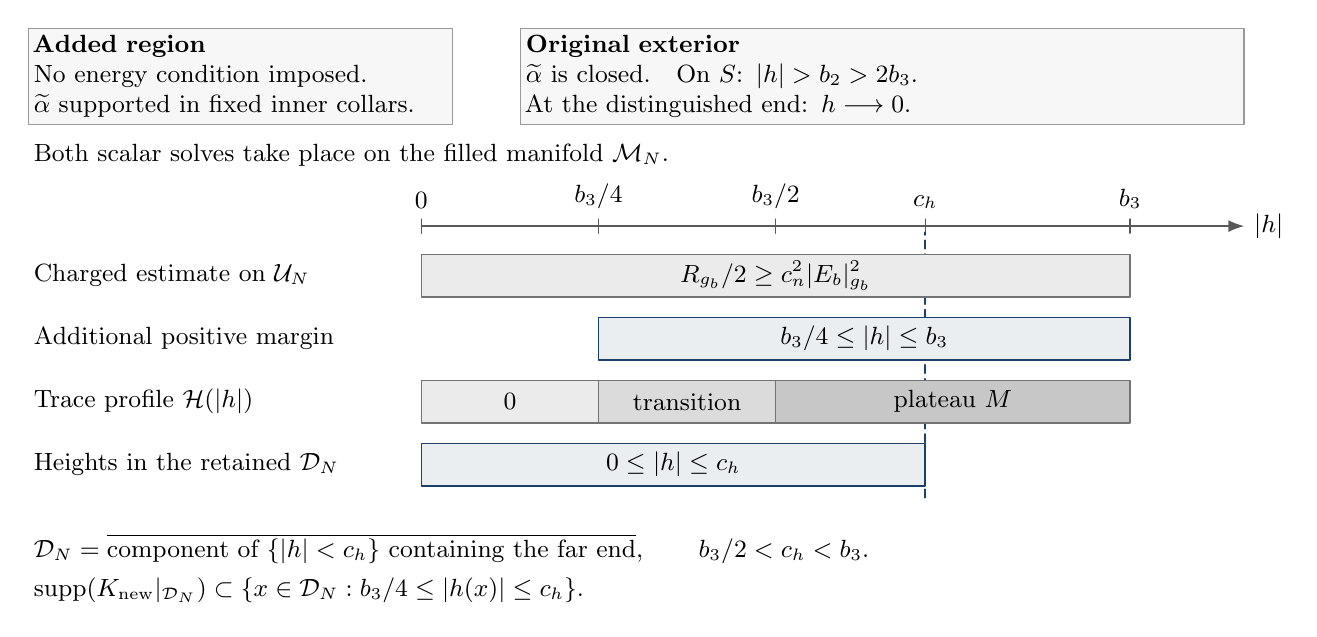
\begin{tikzpicture}[x=1cm,y=1cm,font=\small,
  line cap=round,line join=round,
  every node/.style={inner sep=2pt},
  axis/.style={draw=black!65,line width=.5pt},
  band/.style={draw=black!55,fill=black!8,line width=.45pt},
  focus/.style={draw=linkblue,fill=linkblue!9,line width=.6pt}]
  \node[draw=black!40,fill=black!3,anchor=north west,
    text width=5.25cm,minimum height=1.22cm,align=left]
    at (0,6.4) {\textbf{Added region}\\
      No energy condition imposed.\\
      $\widetilde\alpha$ supported in fixed inner collars.};
  \node[draw=black!40,fill=black!3,anchor=north west,
    text width=9.05cm,minimum height=1.22cm,align=left]
    at (6.25,6.4) {\textbf{Original exterior}\\
      $\widetilde\alpha$ is closed.\quad
      On $S$: $|h|>b_2>2b_3$.\\
      At the distinguished end: $h\longrightarrow0$.};
  \node[anchor=west] at (0,4.78)
    {Both scalar solves take place on the filled manifold $\mathcal M_N$.};

  \draw[axis,-{Latex[length=2mm]}] (5,3.88)--(15.45,3.88);
  \node[anchor=west] at (15.5,3.88) {$|h|$};
  \foreach \x/\lab in {5/0,7.25/{b_3/4},9.5/{b_3/2},11.4/{c_h},14/{b_3}} {
    \draw[axis] (\x,3.79)--(\x,3.97);
    \node[anchor=south] at (\x,4.02) {$\lab$};
  }
  \draw[draw=linkblue,densely dashed,line width=.7pt]
    (11.4,.43)--(11.4,3.8);
  \node[anchor=west] at (0,3.25) {Charged estimate on $\mathcal U_N$};
  \draw[band] (5,2.98) rectangle (14,3.52);
  \node at (9.5,3.25) {$R_{g_b}/2\geq c_n^2|E_b|_{g_b}^2$};

  \node[anchor=west] at (0,2.45) {Additional positive margin};
  \draw[focus] (7.25,2.18) rectangle (14,2.72);
  \node at (10.625,2.45) {$b_3/4\leq |h|\leq b_3$};

  \node[anchor=west] at (0,1.65) {Trace profile $\mathcal H(|h|)$};
  \draw[band] (5,1.38) rectangle (7.25,1.92);
  \draw[band,fill=black!14] (7.25,1.38) rectangle (9.5,1.92);
  \draw[band,fill=black!22] (9.5,1.38) rectangle (14,1.92);
  \node at (6.125,1.65) {$0$};
  \node at (8.375,1.65) {transition};
  \node at (11.75,1.65) {plateau $M$};

  \node[anchor=west] at (0,.85) {Heights in the retained $\mathcal D_N$};
  \draw[focus] (5,.58) rectangle (11.4,1.12);
  \node at (8.2,.85) {$0\leq |h|\leq c_h$};

  \node[anchor=north west,align=left,text width=15.85cm] at (0,.05)
    {$\displaystyle
      \mathcal D_N=\overline{\text{component of }\{|h|<c_h\}
      \text{ containing the far end}},\qquad b_3/2<c_h<b_3.$\\[3pt]
     $\displaystyle
      \supp(K_{\mathrm{new}}|_{\mathcal D_N})
      \subset\{x\in\mathcal D_N:b_3/4\leq |h(x)|\leq c_h\}.$};
\end{tikzpicture}
\caption{Height bands and the late neutral cut. The bars refer only to the
original exterior and encode height, not distance or the topology of level
sets. The end component $\mathcal D_N$ stays outside the filling; every
component of its boundary is retained. After the two scalar solves and the
regular choice of $c_h$, the finite plateau $M$ is chosen to make that
boundary strictly future trapped, without changing $N$ or either solution.
See \eqref{flux:height-separation}--\eqref{flux:low-region},
Lemma~\ref{flux:trace-tensor}, and \eqref{flux:strict-new-boundary}.}
\label{flux:fig-height-bands}
\end{figure}


\begin{proposition}[Prepared numerical bound]
\label{flux:prepared-bound}
For the prepared data, for every $0<s<1$,
\begin{equation}
 \mathcal E_*\geq s|Q|+\frac{1-s^2}{2}X_*.
 \label{flux:prepared-inequality}
\end{equation}
The conclusion also holds for prepared data carrying a smooth compactly
supported closed magnetic two-form, with the charged energy convention
used in the filled scalar construction.
\end{proposition}

\begin{proof}
Keep $s$, a smooth profile, and $\varepsilon$ fixed.  Take $N$ sufficiently
large for all preceding constructions.  Sard's theorem gives a regular
value $c_h\in(b_3/2,b_3)$ of $|h|$.  Let $\mathcal D_N$ be the closure of
the component of $\{|h|<c_h\}$ containing the entire far end.
By \eqref{flux:height-separation}, this component cannot cross $S$ into the
filling.  Its entire boundary is a compact smooth embedded two-sided
hypersurface in the original interior.  It is nonempty: a path in the
original connected exterior from the far end to $S$ must cross the chosen
level.  All boundary components are retained.

The mean curvature of this fixed compact boundary in $\gamma$ is finite.
We may now choose the plateau $M$ in Lemma~\ref{flux:trace-tensor} so large
that, with normal toward the end,
\begin{equation}
 H_{\partial\mathcal D_N}
       +\operatorname{tr}_{\partial\mathcal D_N}K_{\mathrm{new}}
 =H_{\partial\mathcal D_N}-k\mathfrak a<0
 \quad\hbox{on every component}.
 \label{flux:strict-new-boundary}
\end{equation}
This late choice does not require repeating either scalar solve or
increasing $N$, by \eqref{flux:ramp-uniformity}.  Restricted to
$\mathcal D_N$, the new tensor has compact support, since $h\to0$ and
$\mathcal H$ vanishes near zero.

We check the neutral input's hypotheses explicitly.  The exterior
$\mathcal D_N$ is connected and oriented, smooth up to its nonempty compact
boundary, and has exactly the original coordinate end with compact
complement.  It is complete with boundary included: it is closed in the
original complete exterior, and \eqref{flux:metric-dominance} bounds its
metric below by a positive constant times $g$.  The metric is smooth and
has all-order differentiated decay of order $2-n$ in normalized end
coordinates.  Thus the metric and tensor satisfy the stronger falloffs in
Theorem~\ref{thm:neutral-input}, with any exponent strictly between
$(n-2)/2$ and $n-2$.  The neutral DEC follows from
Lemma~\ref{flux:trace-tensor}; its matter densities are integrable because
the tensor is compactly supported and the scalar curvature is integrable
at infinity.  The ADM momentum is zero.  The ADM energy exists and is
given by \eqref{flux:mass-decrease}.  Finally the new boundary is strictly
future outer trapped by \eqref{flux:strict-new-boundary}.

Every full cut of $\mathcal D_N$, regarded as a subset of the original
exterior, is also a full cut there.  This includes any portions coincident
with $\partial\mathcal D_N$, and counts every component.  Therefore its
full-cut infimum $a_N$ satisfies
\begin{equation}
 a_N\geq e^{ky_0}a_*>0.
 \label{flux:area-retention}
\end{equation}
Indeed the metric comparison acts on all $k$ tangent directions, and the
class of available cuts has only been restricted.  No minimizing boundary
is assumed to be smooth or to exist.

It remains to verify the timelike energy hypothesis of the neutral input
for these auxiliary data.  Write $e_N=\mathcal E(\gamma)$.  If $e_N>0$,
their zero momentum makes that hypothesis immediate.  If $e_N\leq0$,
apply the conformal end increase of Lemma~\ref{prep:end-increase}, taking
its positive function $\phi$ constant on a core containing the boundary
and the new tensor's support.  For $U=1+\lambda\phi$, transform the data by
\begin{equation}
 \gamma_\lambda=U^{4/(n-2)}\gamma,
 \qquad K_\lambda=U^{2/(n-2)}K_{\mathrm{new}}.
 \label{flux:neutral-end-increase}
\end{equation}
The neutral DEC and trapping signs persist, the stronger asymptotic
derivatives persist, momentum remains zero, and full-cut areas do not
decrease.  Its energy is $e_N+2\lambda$.  For every arbitrarily small
$e>0$ choose $\lambda=(e-e_N)/2\geq0$.  These data satisfy all hypotheses
of Theorem~\ref{thm:neutral-input}, which would give
\begin{equation}
 e\geq\frac12(a_N/\omega)^{(k-1)/k}
 \geq\frac12e^{(k-1)y_0}X_*>0.
 \label{flux:nonpositive-contradiction}
\end{equation}
Letting $e\downarrow0$ is a contradiction.  Thus $e_N>0$, and the same
neutral input applied directly gives
\begin{equation}
 e^{(k-1)\varepsilon}(\mathcal E_*+o_N(1))
 -\frac{H_0(0)}k|Q|
 \geq\frac12 e^{(k-1)y_0}X_*
 =\frac{1-s^2}{2}X_*.
 \label{flux:prelimit-bound}
\end{equation}

The parameter order is as follows.  For the fixed prepared data, fix
$s\in(0,1)$, a profile tolerance, and $\varepsilon>0$ first.  Complete the
two scalar solves and the regular cut for each sufficiently large $N$;
the tensor plateau is chosen last for that $N$.  Now let $N\to\infty$ in
\eqref{flux:prelimit-bound}, then let $\varepsilon\downarrow0$, and then
let the profile tolerance decrease to zero.  Equations
\eqref{flux:profile-value} and \eqref{flux:floor} give
\eqref{flux:prepared-inequality}.  Only fixed-parameter estimates were
required in the second scalar solve.  The electromagnetic input used in
this proof was precisely \eqref{flux:graph-form-norm} and its lower bound
by $I_g(w)$, which also holds for the indicated compact magnetic form.
\end{proof}

\subsection{Return to the original data and optimize}

\begin{corollary}[Strict compact-magnetic numerical extension]
\label{flux:magnetic-extension}
Let the original exterior satisfy the numerical geometric and asymptotic
hypotheses, and let $D_m$ be an arbitrary smooth compactly supported closed
two-form.  With $\alpha=i_E\vol_g$ closed, use the electromagnetic convention
\begin{equation}
 I_g(v)=c_n^2\bigl(|E|_g^2+|D_m|_g^2+2D_m(v,E)\bigr),
 \qquad
 \mu_m+J_m(v)=\mu+J(v)-I_g(v).
 \label{flux:magnetic-convention}
\end{equation}
Assume also that $\mu_m,|J_m|_g$ are integrable and that the ADM and
charge flux limits exist with the stated normalizations.  Assume the ADM
vector is future timelike, the fixed componentwise trapping
inequalities are strict, and for some $c>0$ and
$0<\beta<\min(1,q)$,
\begin{equation}
 \mu_m-|J_m|_g\geq c r^{-n-\beta}.
 \label{flux:strict-magnetic-margin}
\end{equation}
Then, with the original full-cut infimum $a$ and the original normalized
electric charge $Q$,
\begin{equation}
 m\geq s|Q|+\frac{1-s^2}{2}X_A\quad(0<s<1).
 \label{flux:magnetic-s-family}
\end{equation}
Equivalently, $m\geq|Q|$, and when $X_A>|Q|$ one also has
$m\geq(X_A+Q^2/X_A)/2$.  No magnetic equality classification or
non-timelike extension is asserted here.
\end{corollary}

\begin{proof}
Apply the rest preparation and strict preparation in
Proposition~\ref{prep:rest-preparation} and
Lemma~\ref{prep:strictification}, retaining the two closed forms.  The
magnetic support stays in the compact original region.  There the strictly
positive margin absorbs the arbitrarily small rescaling errors.  The
gluing and bending annuli can be taken outside that support, so on those
annuli and on the end the electric estimates are unchanged.  This yields
prepared data with charge $Q$, energies $\mathcal E_{*,j}\to m$, and
full-cut infima $a_{*,j}\geq(1-o_j(1))a$.  For each fixed $s$, apply
Proposition~\ref{flux:prepared-bound} and then pass to this limit.  The
right side is increasing in the area variable, so the lower comparison of
infima is sufficient.  This proves \eqref{flux:magnetic-s-family}.  The
elementary optimization is given in
Proposition~\ref{prep:prepared-reduction}.  The argument does not require
the component electric fluxes to have one sign.
\end{proof}

\begin{proof}[Completion of Theorem~\ref{thm:numerical}]
Proposition~\ref{flux:prepared-bound} establishes
\eqref{prep:prepared-bound-hypothesis} for every prepared data set
with positive energy and zero momentum, and every fixed $s\in(0,1)$.
The Reduction of the Numerical Theorem
(Proposition~\ref{prep:prepared-reduction}) therefore proves
Theorem~\ref{thm:numerical}, including positivity of the full enclosing
area, strict future timelikeness of the original ADM vector, and the
stated branch distinction. The endpoint limits in $s$ are taken after
the fixed-$s$ inequality is established, so no profile estimate uniform
at $s=0$ or $s=1$ is required.
\end{proof}

\section{The original-data variational identity}
\label{var:section}

We now assume the connected-horizon hypotheses of
Definition~\ref{def:rigidity-class} and equality in
Theorem~\ref{thm:numerical}, with $m>|Q|$.  All objects in this section
belong to the original exterior $(\Omega,g,K,E)$.  In particular, no
equality statement about one of the auxiliary metrics is used.  We first
differentiate the full enclosing-area infimum, then separate the active
constraint inequalities from a direction that would improve equality.
The resulting multipliers are initially measures.  Their regularity and
the elimination of their possible singular area sheets are separate
steps.
Decrease the asymptotic exponent, if necessary, so that
$(n-2)/2<q<n-2$; this retains every original hypothesis.

Write $A=\Area_g(S)$, $k=n-1$, and
\begin{equation}
 r_h=(A/\omega)^{1/k},\qquad
 b^0=\frac{\mathcal E_{\mathrm{ADM}}}{m},\qquad
 b^i=-\frac{(\mathbf P_{\mathrm{ADM}})_i}{m},\qquad
 c=\frac{k-1}{r_h}\left(1-\frac{Q^2}{r_h^{2(k-1)}}\right)>0.
 \label{var:constants}
\end{equation}
The vector $b$ is fixed when taking variations.  Set
$\mathcal B=b^0\mathcal E_{\mathrm{ADM}}+\sum_i b^i
(\mathbf P_{\mathrm{ADM}})_i$.  Thus $m'=\mathcal B'$ at the original
data.  On the outer, nonextremal area branch, differentiation at fixed
$Q$ gives
\begin{equation}
 \frac{\dd}{\dd A}\frac12
 \left(r_h^{k-1}+Q^2r_h^{-(k-1)}\right)
 =\frac{c}{2k\omega}.
 \label{var:area-coefficient}
\end{equation}
The strictly positive coefficient in this formula will be essential.

Throughout the variations, an electric field is represented by the
closed flux form $\alpha=i_E\vol_g$.  We also allow a closed, compactly
supported two-form $D_m$, initially zero, representing the spatial
Faraday form divided by $c_n$.  For these extended data put
\begin{equation}
 \begin{split}
 \mu_m&=\frac12(R_g+\tau^2-|K|^2)
              -c_n^2(|E|^2+|D_m|^2),\\
 J_m&=\operatorname{div}(K-\tau g)-2c_n^2D_m(\,\cdot\,,E).
 \end{split}
 \label{var:magnetic-constraints}
\end{equation}
Only the strictly feasible numerical extension of
Corollary~\ref{flux:magnetic-extension} will be applied to data with
$D_m\ne0$.  No magnetic equality theorem is assumed.  Compactly
supported closed variations of either form, including tests supported
up to $S$, do not change $Q$, by Stokes' theorem on a truncation.

\subsection{The full area envelope}

Choose a compact smooth filling $O$ behind $S$, with a smooth extension
of the metric, and denote the resulting boundary-free manifold by
$\mathcal M$.  The filling is used only to define perimeter
competitors; no constraint inequality is required there.  A filled
competitor is a bounded finite-perimeter set $F\subset\mathcal M$
containing $O$ up to null sets.  Its perimeter counts the part coinciding
with $\partial O=S$.

\begin{proposition}[Area envelope and regular patches]
\label{var:area-envelope}
The least perimeter of filled competitors equals the full smooth-cut
infimum $a$.  The family $\mathcal F_*$ of minimizing filled sets,
considered modulo null sets, is compact in local $L^1$, and all its
members are supported in a common compact set.  Their exterior end
components have the full-boundary convention of
Definition~\ref{def:full-cut}.

Each minimizing frontier is smooth and minimal at its free regular
points.  Its possible singular set has Hausdorff dimension at most
$n-8$.  All contact points with $S$ are regular of class $C^{1,\gamma}$
for some $\gamma>0$, and their graph representations belong to
$W^{2,p}$ for every finite $p$.  At an interior regular point of one
frontier, any other minimizing frontier through the point coincides
with it locally.  On a smaller neighborhood the minimizing frontiers
that meet that neighborhood are disjoint single graphs, with uniform
smooth interior estimates.

For a differentiable metric path with $g'_0=h$, the right derivative
of its enclosing-area infimum is
\begin{equation}
 a'_+(h)=\min_{F\in\mathcal F_*} a'_F(h),\qquad
 a'_F(h)=\frac12\int_{\partial^*F}
                       \operatorname{tr}_{T\partial^*F}h\,\dd A_g.
 \label{var:envelope-derivative}
\end{equation}
Here and below $\partial^*F$ is used for integration, while
``frontier'' means the support of its perimeter measure.
\end{proposition}

\begin{proof}
Large coordinate spheres have positive mean curvature, uniformly for
the finite-dimensional metric paths considered below.  On the region
outside one such sphere, the outward unit normal to their foliation
has positive divergence.  Applying the divergence theorem to the
portion of a filled competitor outside that sphere shows that clipping
off that portion cannot increase perimeter, and strictly decreases it
if the discarded portion has positive volume.  The argument holds for
almost every cutting radius by finite-perimeter slicing.  Choose two
fixed radii, both outside the compact core.  Clipping at the smaller
radius gives a common compact truncation, strictly inside the larger
one, for minimization and for all sufficiently small parameters of
each path.  BV compactness and lower semicontinuity now give a
minimizer; see \cite{AmbrosioFuscoPallara2000}.

A smooth full cut bounds a filled competitor with exactly the same
area, including its contact portions.  Conversely, first push $O$ and
an arbitrary filled competitor slightly outward by a smooth ambient
diffeomorphism supported in a collar of $S$.  The pushed competitor
contains a neighborhood of the original $O$, and its perimeter tends
to the original perimeter.  Strict approximation of finite-perimeter
sets by smooth domains can therefore be carried out while retaining
that neighborhood.  It is supported inside a fixed compact
truncation.  Retain the exterior component containing the end, filling
any bounded exterior components of the smoothed set.  This only
removes boundary components.  Its entire smooth intrinsic boundary is
a full cut.  Passing through these two approximations proves equality
of the infima.  The same removal observation shows that a minimizing
frontier cannot leave a removable bounded complementary open
component: a nonempty such component has positive perimeter, whose
removal would improve the minimum.  The usual indecomposable-component
decomposition gives the same conclusion for finite-perimeter
representatives \cite{AmbrosioFuscoPallara2000}.

Here is the local estimate needed at the obstacle.  For a local
competitor $G$, replace it by $G\cup O$.  Submodularity gives
\begin{equation}
 P(G\cup O)\le P(G)+P(O)-P(G\cap O).
 \label{var:obstacle-submodularity}
\end{equation}
Extend the smooth outward normal of $O$ to a smooth vector field of
norm at most one near its boundary.  Its divergence is bounded.
The calibration inequality for this field gives
$P(O)-P(G\cap O)\le C|O\setminus G|$ for changes in a sufficiently
small coordinate neighborhood.  Since $F$ minimizes among sets
containing $O$, it follows that
\begin{equation}
 P(F;B)\le P(G;B)+C|F\mathbin{\triangle}G|
 \label{var:quasiminimizing}
\end{equation}
whenever $F\mathbin{\triangle}G$ is compactly contained in the small
ball $B$.  This is an unconstrained perimeter almost-minimizing
estimate.  In coordinates the Riemannian area integrand is the
ellipsoidal integrand associated with
$\mathcal A=(\det g)g^{-1}$, which is smooth and uniformly elliptic.
The error in \eqref{var:quasiminimizing} is $O(r^n)$ and therefore is
bounded by $C_\gamma r^{n-1+\gamma}$ for any fixed
$0<\gamma<1$ on sufficiently small balls.  The almost-minimizer results in
\cite[Propositions~4.5--4.7 and Theorems~1.1, 9.5,
10.2--10.3]{Simmons2022} apply.  They give density and perimeter
bounds, local compactness, regularity off a set of dimension at
most $n-8$, and convergence as single $C^1$ graphs near free
regular limit points.  On free patches, the uniform local
$C^{1,\gamma/4}$ graph bounds and the smooth minimal-graph
equation upgrade this to smooth convergence on smaller patches
by interior elliptic estimates.  Tangent sets are
perimeter-minimizing cones.  The minimal-boundary formulation and
dimension reduction are also described in
\cite[Chapter 7, Section 5]{SimonGMT2014}.

At a contact point a tangent filled cone contains the tangent
half-space of $O$.  The corresponding minimizing hypercone is
therefore supported on one side of its boundary plane, and is that
plane.  One way to see the last assertion is to integrate the signed
coordinate-height equation on its stationary spherical link; the
height has one sign and its spherical Laplacian is a negative
constant times itself.  The singular set can be removed in this
integration by its dimension and the perimeter bounds.  Equivalently
one can use the half-space cone theorem in
\cite[Chapter~7, Section~4, Theorem~4.5]{SimonGMT2014}.  The almost-minimizer
regularity theorem now gives a $C^{1,\beta}$ graph at contact
for some $\beta>0$; one may take $\beta=\gamma/4$.
Estimate~\eqref{var:quasiminimizing}, differentiated along smooth
flows, bounds its weak mean curvature.  Difference quotients in the
uniformly elliptic prescribed-mean-curvature graph equation give
$W^{2,2}$ regularity.  Written in nondivergence form, that equation
has H\"older coefficients and bounded right-hand side, so local
$W^{2,p}$ estimates give all finite $p$; see
\cite{GilbargTrudinger2001}.

If two minimizing frontiers meet at a free regular point of one of
them, their union and intersection also minimize by
\eqref{var:obstacle-submodularity}, with equality in the sum of the
perimeters.  They are ordered relative to the given regular sheet.
Their tangent cones at contact are one-sided relative to its tangent
plane, and hence are planes.  Regularity and the strong comparison
principle for the minimal graph equation imply local coincidence.
Strict compactness and regular convergence then give the asserted
uniform graph neighborhoods: otherwise a sequence of failing
frontiers would converge strictly to a minimizer through the point,
where multiplicity-one regular convergence gives precisely the
missing neighborhood.  The difference of two distinct ordered
graphs solves a linear uniformly elliptic equation.  Positive-solution
Harnack and interior derivative estimates imply, on smaller patches,
that its gradient is bounded by a uniform constant times its
pointwise separation.

Finally let $F_t$ minimize for $g_t$.  Compactness, lower
semicontinuity and comparison with a fixed $g_0$ minimizer show that
every convergent subsequence at $t=0$ converges strictly in perimeter
to an element of $\mathcal F_*$.  Strict continuity for vector
measures then gives convergence of the tangent-plane area measures
\cite{AmbrosioFuscoPallara2000}.  The area Taylor expansion has a
uniform remainder on the resulting perimeter-bounded family.  Fixed
minimizers give the upper bound in
\eqref{var:envelope-derivative}; the varying minimizers give the lower
bound.  This also proves compactness of the minimizing family and
continuity of $F\mapsto a'_F(h)$ in its strict topology.
\end{proof}

\subsection{Strict directions and positive-measure separation}

An active ray is a pair $(x,v)$ with $|v|_g\le1$ and
$\mu_m(x)+J_m(x)(v)=0$.  Under a metric variation $h$, transport the
unit ball by the metric square root, so $v'=-h^\sharp v/2$.  Denote by
$\mathfrak C'$ the variation of $2(\mu_m+J_m(v))$ under that
transport.  Our test space consists of finite linear combinations of:
\begin{enumerate}[label=(\roman*)]
 \item arbitrary compact smooth variations $(h,p,\alpha',D_m')$,
 including support up to $S$, with $p=K'$ and both form variations
 closed;
 \item a metric end prototype $h=r^{2-n}\delta$, cut off toward the
 core;
 \item second-tensor end prototypes whose Euclidean trace reversal is
 \begin{equation}
  \Pi_{ij}=r^{-k}
   \bigl(a_i n_j^\delta+a_j n_i^\delta
                     -(a\cdot n^\delta)\delta_{ij}\bigr),
  \qquad n^\delta=x/r,
  \label{var:momentum-prototype}
 \end{equation}
 with arbitrary constant $a\in\R^n$ and a cutoff toward the core;
 \item the strict conformal direction $(h,p)=(2\phi g,\phi K)$,
 with both forms fixed.
\end{enumerate}
For the last direction choose $0<\beta<\min(1,q)$, put
$\rho_0=r^{-n-\beta}$ with a positive smooth extension of the radial
weight, and take
\begin{equation}
 -\Delta\phi=B\sqrt{|\dd\phi|^2+r^{-2k}}+\rho_0,
 \qquad \partial_\nu\phi=-1,
 \qquad \phi(\infty)=0,
 \label{var:strict-direction}
\end{equation}
where $B\ge |K|$ is smooth and has simple symbol bounds
$B=O_j(r^{-1-q})$.  The strictification construction in
Lemma~\ref{prep:strictification} applies to this decaying drift:
its radial barriers dominate the drift because $\beta<q$.  It gives
$\phi>0$, $\phi=O_2(r^{2-n})$ and finite gradient flux.  In
particular
\begin{equation}
 \frac{-\Delta\phi}{\rho_0}\longrightarrow1,
 \qquad
 \frac{\mathfrak C'_{\rm strict}}{\rho_0}>0
 \text{ on active rays},\qquad
 \frac{\mathfrak C'_{\rm strict}}{\rho_0}\longrightarrow2k,
 \qquad -\theta'_{\rm strict}=k.
 \label{var:strict-tail}
\end{equation}
Here the extra algebraic electric term is nonnegative: at a purely
electric active ray the conformal derivative of $\mathfrak C$ is
\begin{equation}
 -2k\Delta\phi+2kK(\nabla\phi,v)
                  +4(k-1)c_n^2\phi|E|^2.
 \label{var:conformal-active-derivative}
\end{equation}

The prototypes have zero flat linearized constraints on the end.
For example
$\Pi_{ij}=r^{-n}(a_ix_j+a_jx_i-(a\cdot x)\delta_{ij})$
satisfies $\partial_j\Pi_{ij}=0$ and
$\Pi_{ij}n^j=r^{-k}a_i$.  Its momentum derivative is $a_i/k$;
the scalar prototype has energy derivative $(n-2)/2$.
The background errors in the linearized constraints are
$O(r^{-n-q})$.  Thus the prototypes span the ADM flux derivatives
and their normalized active-constraint values tend to zero.

\begin{proposition}[Multiplier identity]
\label{var:multiplier-identity}
There are a probability measure $\pi$ on $\mathcal F_*$, a
nonnegative locally finite measure $\Lambda$ on the active rays,
and a nonnegative finite measure $\zeta$ on $S$, such that
\begin{equation}
 2k\omega\mathcal B'-c\int_{\mathcal F_*}a'_F(h)\,\dd\pi(F)
 =\int\mathfrak C'\,\dd\Lambda-\int_S\theta'_+\,\dd\zeta
 \label{var:separation}
\end{equation}
for every compact test and every end prototype above.  No
surjectivity of a constraint map is required.
\end{proposition}

\begin{proof}
Consider the linear image of the test space with components
\begin{equation}
 \left(\mathfrak C'/\rho_0,\ -\theta'_+,\
       \{c a'_F(h)-2k\omega\mathcal B'\}_{F\in\mathcal F_*}\right).
 \label{var:separation-map}
\end{equation}
The constraint test space is the one-point compactification of the
closed active-ray set, with one artificial infinity point added even
if that set is bounded.  At infinity assign $2k$ times the
coefficient of the strict direction.  The other two test spaces are
$S$ and the compact minimizing family.  The normalized functions
are continuous by \eqref{var:strict-tail} and
Proposition~\ref{var:area-envelope}.

This image does not meet the open cone of functions strictly
positive on the disjoint union of the three compact test spaces.
Indeed such a direction has positive strict-direction coefficient
because of the infinity test.  Apply that positive conformal
direction exponentially to the data after making the other
variations additively.  On compact subsets, strict first-order
positivity on the active rays implies feasibility for all
sufficiently small positive parameters: rays outside a fixed
neighborhood of the active set have a positive zeroth-order gap.
On the end the nonconformal linear errors are $O(r^{-n-q})$ and
are dominated by $\rho_0$.  After retaining the nonnegative
background through the conformal formula, the quadratic errors are
bounded by $Ct^2\rho_0$.  The strict first-order term therefore
gives $\mu_m-|J_m|\ge c_t\rho_0$, with $c_t>0$.
The forms remain closed; a newly created magnetic form has fixed
compact support.  Trapping is strict, the ADM vector remains
future timelike, and completeness, decay, integrability and
existence and differentiability of the fluxes are preserved.
These are precisely the hypotheses of
Corollary~\ref{flux:magnetic-extension}.  The area infimum stays
positive by uniform metric comparison on the compact core and
the controlled tail.  Equation~\eqref{var:envelope-derivative}
and strict positivity of the objective components would now
violate the numerical inequality for small positive parameter.

Hahn--Banach separation of a linear subspace from an open convex
cone gives a nonzero positive functional on the continuous
functions on this compact disjoint union.  The Riesz
representation theorem supplies the three nonnegative measures.
Its objective measure has positive mass.  Otherwise testing the
strict direction, uniformly positive on the two constraint test
spaces, would force both remaining measures to vanish as well.
Normalize the objective measure to have mass one.  On finite
active rays divide the constraint measure by $\rho_0$ to obtain
$\Lambda$.  This measure is finite over compact subsets,
including the boundary.  The possible infinity atom contributes
nothing on compact tests or prototypes.  Rearranging the
annihilation identity gives \eqref{var:separation}.
\end{proof}

\subsection{Normal-motion tests and the sheets selected by the multiplier}

Let $u$ and $X$ be the scalar and vector moments of $\Lambda$.
Initially these are measures, using the fixed Riemannian
volume-density convention; thus $u$ also denotes the scalar
distribution defined by its moment measure.  Positivity and the
definition of the active set imply
\begin{equation}
 u\ge |X|_g,\qquad u\mu_m+J_m(X)=0
 \label{var:moment-complementarity}
\end{equation}
as measure identities.  In particular, electromagnetic or
metric terms of the ray derivative require moments of order at
most one.

\begin{lemma}[Tangential trace on free sheets]
\label{var:trace-free-sheets}
For $\pi$-almost every minimizing frontier,
$\operatorname{tr}_{T\partial F}K=0$ on each of its free regular
sheets.  Every such frontier either equals $S$, or is wholly
inside $\operatorname{int}\Omega$ and satisfies
$H=\operatorname{tr}_{T\partial F}K=0$ on its regular part.
\end{lemma}

\begin{proof}
Fix a smooth lapse test $s$ compactly supported in the open
exterior, and choose a local Gaussian Lorentzian metric inducing
$g,K$ at time zero.  Its spatial metric and first normal jet are
fixed, while its second normal metric jets are free.  Choose a
two-form whose initial electric and spatial components are
$c_n E$ and zero.  Its first normal derivatives can be chosen so
that both Maxwell equations hold on the initial slice.  In
general dimension the tangential Maxwell constraints are
$\dd D_m=0$ and $\dd\alpha=0$; the remaining equations prescribe
the $n(n-1)/2$ magnetic and $n$ electric normal evolution
components.  The induced flux-form variations under normal
motion with velocity $sN$ are compactly supported and closed,
as follows also from Cartan's formula applied to these initial
Maxwell jets.

Let $\mathsf S$ denote the electromagnetic stress tensor with
the normalization in Definition~\ref{def:normalization}.
It is divergence-free at the initial slice.  For each
$\delta>0$, prescribe there the spatial components of
Einstein minus $\mathsf S$ to be
\begin{equation}
 T^{(\delta)}_{ij}
       =\frac{(J_m)_i(J_m)_j}{\mu_m+\delta}.
 \label{var:normal-jet-matter}
\end{equation}
Spatial trace reversal of the second normal metric jets is
invertible, so these are legitimate smooth jet prescriptions.
The normal and mixed components remain $\mu_m,J_m$ by
Gauss--Codazzi.  The resulting variation has $h=2sK$.

We check that $\mathfrak C'\to0$ uniformly on compact active
test sets.  The tensors in \eqref{var:normal-jet-matter}
converge spatially in $C^1$.  On $\{\mu_m>0\}$ this is
ordinary smooth convergence; near a zero of $\mu_m$, DEC gives
$|J_m|\le\mu_m$ and smoothness gives
$\dd\mu_m=\nabla J_m=0$ at that zero.  The bounds
\begin{equation}
 |T^{(\delta)}|\le\mu_m,
 \qquad
 |\nabla T^{(\delta)}|
       \le 2|\nabla J_m|+|\dd\mu_m|
 \label{var:matter-jet-bounds}
\end{equation}
make the convergence uniform across the zero set.
At a positive-density active ray, the limiting spacetime tensor
is $\gamma\otimes\gamma/\mu_m$, where
$\gamma(N)=\mu_m$ and $\gamma|_{T\Omega}=J_m$.
It is causal and annihilates the null vector $N+v$.
Parallel-transport that null vector along spatial curves.
Its contraction with the causal covector is nonnegative and
vanishes at the base point; differentiation at the minimum
therefore shows that all relevant spatial covariant
derivatives, with last argument $N+v$, vanish.  Bianchi and the
initial Maxwell equations then give the same limiting
vanishing for the normal derivative contracted with
$N,N+v$.  Changes of the first argument cost zero, and changes
of the second cost zero because it remains null and
$\gamma$ is proportional to its metric dual.  At a matter
zero, both the tensor and its spatial derivatives vanish by
\eqref{var:matter-jet-bounds}, and the divergence equation
again suffices.  These observations prove the asserted uniform
convergence of $\mathfrak C'$.

Apply \eqref{var:separation} to these tests and pass to the
limit.  They have no boundary or ADM variation, so
\begin{equation}
 \int_{\mathcal F_*}\int_{\partial^*F}
       s\operatorname{tr}_{T\partial^*F}K\,\dd A_g\,\dd\pi(F)=0.
 \label{var:weighted-trace-zero}
\end{equation}
At free regular points, Proposition~\ref{var:area-envelope}
provides uniform noncrossing graph patches, and frontiers
through a common point have the same tangent plane.
Consequently the tangential trace is a single-valued
continuous function on each such patch of the integrated
surface measure.  There is no cancellation between different
tangent planes in \eqref{var:weighted-trace-zero}.
A countable cover and Fubini imply the first conclusion,
initially almost everywhere and then everywhere on regular
sheets by smoothness.

At contact, the $W^{2,p}$ graph and the smooth obstacle have
the same second jets almost everywhere on their coincidence
set.  The frontier therefore satisfies
$H+\operatorname{tr}_{\rm tan}K=0$ almost everywhere throughout
the contact graph, including its free portion.  Uniform
ellipticity first improves its regularity and then bootstraps
it to a smooth solution of the expansion equation.  The
strong comparison principle gives coincidence with $S$ near
contact.  The set of coincidence is open and closed along
the connected $S$, so the whole $S$ is present.  Its area is
already the minimum $A$, leaving no area for another sheet.
If there is no contact, the compact frontier is separated
from $S$, and the stated equations hold on all its regular
points.
\end{proof}

\subsection{The moment equations and their initial regularity}

\begin{proposition}[Regularity of the measure moments]
\label{var:moment-regularity}
In the open exterior the moments are functions satisfying the first Killing initial data (KID) equation
\begin{equation}
 \operatorname{sym}\nabla X=-uK,
 \label{var:first-kid}
\end{equation}
and
\begin{equation}
 \operatorname{Hess}u
  =\mathcal L(u,X,\nabla X)
    +\frac c2\int_{\mathcal F_*}
       \nu_F^\flat\otimes\nu_F^\flat\,
                       \dd A_F\,\dd\pi(F).
 \label{var:hessian-measure}
\end{equation}
The equations are distributional, and surface measures in the
second equation are expressed relative to ambient volume.
The operator $\mathcal L$ has smooth linear coefficients.
It is specifically the lower-order operator from the metric
adjoint in \eqref{var:separation}, with the flux form fixed
and the unit-ball rays transported as specified above.
In particular, it is not an arbitrary operator with smooth
coefficients.  Locally $u$ is Lipschitz and $X$ is $C^{1,1}$.
The complementarity relations
\eqref{var:moment-complementarity} hold pointwise.
\end{proposition}

\begin{proof}
For a compactly supported interior variation $K'=p$, the
coefficient after integration by parts is
\begin{equation}
 2\bigl[u(\tau g-K)-\operatorname{sym}\nabla X
                                  +(\operatorname{div}X)g\bigr]:p.
 \label{var:second-tensor-adjoint}
\end{equation}
Its trace gives $\operatorname{div}X=-u\tau$, and its
trace-free part then gives \eqref{var:first-kid}.
For metric tests the scalar-curvature principal adjoint is
$\operatorname{Hess}u-(\Delta u)g$.
Connection variations in the momentum term give smooth
linear expressions in $u,X,\nabla X$; fixed-flux field terms
and the ray-transport term are algebraic in those moments.
The area term has coefficient
$-c(g-\nu_F^\flat\otimes\nu_F^\flat)/2$ on this side of
\eqref{var:separation}.  Inverting trace reversal gives
\eqref{var:hessian-measure}, with the displayed positive
normal-normal measure.

Differentiating \eqref{var:first-kid} and commuting
covariant derivatives expresses every component of
$\nabla^2X$ as a smooth linear combination of
$\operatorname{Rm}*X$, $K*\dd u$ and $(\nabla K)*u$.
Taking traces gives a strongly elliptic Laplace system for
$(u,X)$ with smooth lower-order coefficients.  Its source
measure has local growth $O(r^{n-1})$, uniformly in the
minimizer, by the local perimeter bound.  A localized
elliptic parametrix has order $-2$ and kernel bounds
$C|x-y|^{2-n-j}$ for $j=0,1$.  Such a potential of a measure
with this growth is locally $C^\gamma$ for every
$0<\gamma<1$: split the potential difference at twice the
point separation, use the growth bound nearby and the
first kernel derivative on successive outer annuli to get
$O(r(1+|\log r|))$.  Lower-order terms are included in the
parametrix, and the homogeneous remainder is smooth.
Thus $u,X$ are H\"older continuous.

The traced differentiated equation for $X$ now has the
form of the divergence of a H\"older field plus a
H\"older function; local elliptic estimates give
$X\in C^{1,\gamma}$, after decreasing $\gamma$ if needed.
The lower term in \eqref{var:hessian-measure} is therefore
continuous.  Its positive measure term implies a local
lower bound for the covariant Hessian in the distributional
sense.  Slice this inequality in smooth flow boxes whose
longitudinal curves are unit-speed geodesics.  Multiplying
by the smooth volume Jacobian gives the one-dimensional
distributional inequality $(u\circ\gamma)''\ge-C$ on
almost every such curve.  Continuity extends its integrated
convexity inequality to every curve in a smaller box.
This is local geodesic semiconvexity, which implies a local
Lipschitz bound by bounding one-sided slopes on short
geodesic segments with endpoints in a fixed larger ball.
The differentiated
equation for $X$ consequently has bounded right-hand
side componentwise, so $\nabla^2X$ is locally bounded and
$X\in C^{1,1}$.  The measure inequalities now reduce to
pointwise inequalities by continuity.
\end{proof}

For clarity about the field coefficients in this adjoint,
holding $\alpha=i_E\vol_g$ fixed gives
$E'=-(\operatorname{tr}h)E/2$ and hence
\begin{equation}
 \delta\bigl(2u c_n^2|E|^2\vol_g\bigr)
   =u c_n^2\bigl(2E_iE_j-|E|^2g_{ij}\bigr)h^{ij}\vol_g
   =-u\mathsf S_{ij}h^{ij}\vol_g.
 \label{var:electric-metric-adjoint}
\end{equation}
The ray transport contributes $-(J_m)_{(i}X_{j)}h^{ij}$.
The added variation of volume in the full constraint
pairing is zero by complementarity.  These identities,
together with the actual gravitational adjoint, will
control null focusing in the next section.  In
particular, the singular term in
\eqref{var:hessian-measure} cannot be discarded by
assuming regularity of a minimizing frontier.

\section{Eliminating interior area multipliers}
\label{var:singular-multipliers}

We prove that the area multiplier obtained from separation is concentrated on
the given boundary.  The main issue is that an area minimizer can have a
singular frontier in high dimension.  Atomic transverse mass forces a regular
sheet to be totally geodesic.  For the remaining sheets, a common positive
Jacobi field, null focusing, and a cone argument give a uniform curvature
bound.  A separate locality argument removes diffuse multiplier mass from
sheets on which the lapse vanishes.  All these arguments concern the original
smooth data.

Throughout this section, $k=n-1$, and $\mathcal F_*$ and $\pi$ are the compact
family and probability measure of Proposition~\ref{var:area-envelope} and
equation~\ref{var:separation}.  We use the full-measure family supplied by
Lemma~\ref{var:trace-free-sheets}, intersected with $\operatorname{supp}\pi$.
A member of this family has frontier $S$,
or has compact frontier wholly in the open exterior and satisfies
\begin{equation}\label{var:zero-sheet-expansions}
 H_\Sigma=0,\qquad \operatorname{tr}_\Sigma K=0
\end{equation}
on every free regular sheet.  We retain the local common-sheet,
noncrossing, and graphical compactness conclusions of
Proposition~\ref{var:area-envelope}.  In particular, distinct nearby sheets
are disjoint graphs, and on smaller patches the tilt between them is bounded
by a constant times their separation.

The moments of Proposition~\ref{var:moment-regularity} satisfy
\begin{equation}\label{var:singular-system}
 \operatorname{sym}\nabla X=-uK,\qquad
 \nabla^2u=B(u,X,\nabla X)+\mathcal M,
 \qquad
 \mathcal M=\frac c2\int_{\mathcal F_*}
       \nu_D^\flat\otimes\nu_D^\flat\,dA_D\,d\pi(D)
\end{equation}
in the open exterior.  Here $c>0$, $u$ is locally Lipschitz, $X$ is locally
$C^{1,1}$, and the last formula defines a tensor-valued measure relative to
the smooth volume density.  Its singular sets have zero sheet area.
Here $B$ abbreviates the operator $\mathcal L$ of
Proposition~\ref{var:moment-regularity}.  It is the precise lower-order
metric-adjoint expression in
equation~\ref{var:separation}, with the electric flux held fixed and the
unit-ball rays transported isometrically.  It has smooth coefficients and
is linear in its displayed arguments.  Its origin, and not merely its
regularity, will be used in the focusing calculation.  We also have
\begin{equation}\label{var:singular-complementarity}
 u\geq |X|,\qquad \mu_m\geq |J_m|,\qquad
 u\mu_m+J_m(X)=0.
\end{equation}

\subsection{Local leaf measures and atomic sheets}

Fix a free regular incidence point $(D,p)$.  The uniform graph conclusion
of Proposition~\ref{var:area-envelope}, after shrinking its neighborhood,
provides nested open spatial boxes
\[
 p\in W\Subset V\Subset U,
 \qquad W=B_0\times I_0,
\]
in coordinates $(y,t)$, and a larger base ball $B_1\supset\overline{B_0}$,
with the following property.  Every minimizing frontier that meets $V$
has in $U$ a unique selected graph $t=f_F(y)$ over $B_1$; all portions of
that frontier in $W$ belong to this graph.  Its graph over $B_1$ lies in
the coordinate chart, and the graphs have uniform interior smooth
bounds and are mutually disjoint unless they coincide.  The boxes can
be chosen with this property by first taking the uniform graph
neighborhood and then choosing the middle and inner boxes with positive
margin from its side and top faces.

Put
\[
 \mathcal H_V=\{F\in\mathcal F_*:
                         \operatorname{frontier}(F)\cap V\ne\varnothing\}.
\]
This is an open subset of the minimizing family.  Indeed convergence
in that compact family is strict perimeter convergence, hence its
perimeter measures converge weakly.  If the limit frontier meets the
open set $V$, its perimeter measure is positive on a nonnegative
compactly supported test in $V$, and the same holds for every sufficiently
late member of the sequence.  This proves openness.  The uniform density
bounds also give local Hausdorff convergence of the frontier supports:
a putative boundary point staying a positive distance from the limit
frontier would force positive volumes of both phases in a ball where
the limit is constant, contradicting local $L^1$ convergence.

The graph map
\[
 q_V:\mathcal H_V\longrightarrow C^\infty(B_1),\qquad q_V(F)=f_F,
\]
is continuous for the topology of smooth convergence on compact
subsets.  To see this, apply regular multiplicity-one convergence at
the limiting graph on each compact subball; the uniform graph bounds
and uniqueness identify every subsequential limit.  Define the finite
Borel measure
\[
 \lambda_V=(q_V)_*(\pi|_{\mathcal H_V})
\]
on the entire separable metrizable function space $C^\infty(B_1)$.
This definition identifies coincident local graphs without requiring
the image of $q_V$ to be a Borel subset of that space.  We write
$\mathcal G$ for this leaf-parameter space and $\lambda$ for
$\lambda_V$ when the box is fixed.

Every source contribution on $W$ is retained: a frontier meeting $W$
also meets $V$, and is therefore in $\mathcal H_V$.  No arbitrary
neighborhood of the reference minimizer is used to truncate this
measure.  Distinct realized graph parameters are disjoint, so for each
$y\in B_1$ the map
\begin{equation}\label{var:injective-leaf-evaluation}
 \ell\longmapsto f_\ell(y)
\end{equation}
is injective on the realized leaves.  All integrals with respect to
$\lambda$ mean the corresponding pushforward integrals over
$\mathcal H_V$; the injectivity assertion concerns the realized
graphs in those integrals.

\begin{lemma}[Atomic leaves]\label{var:atomic-leaves}
If $\lambda(\{\ell_0\})>0$, the corresponding regular sheet is
totally geodesic on $\operatorname{graph}(f_{\ell_0})\cap W$.
\end{lemma}

\begin{proof}
Fix any point of $\operatorname{graph}(f_{\ell_0})\cap W$ and take
signed normal-distance coordinates $(y,s)$ about that sheet on a
smaller patch compactly contained in $W$, writing the sheet as
$\Sigma=\{s=0\}$.  Put $m_0=\lambda(\{\ell_0\})>0$.
The $ss$ equation in \eqref{var:singular-system} is a one-dimensional
second-derivative equation after slicing by almost every normal line.
The bounded nonmeasure terms include $B$ and the coordinate connection
terms.  The atom at $s=0$ has coefficient $cm_0/2$: on the reference graph
the unit conormal is $ds$ and the sheet and volume Jacobians agree at
$s=0$.  No other graph produces an atom there, by
\eqref{var:injective-leaf-evaluation}.  Consequently $\partial_su$ has
bounded one-sided traces $v^\pm(y)$ for almost every $y$, and
\begin{equation}\label{var:atomic-normal-jump}
 v^+(y)-v^-(y)=\frac c2m_0.
\end{equation}
The existence and boundedness of these traces can also be read directly
from local semiconvexity of $u$ along the normal lines.

We compare the tangential equations from the two sides.  Let $A_s$ be the
second fundamental form of the parallel sheet $\{s=\mathrm{constant}\}$,
with normal $\partial_s$.  With $A_s(V,W)=g(\nabla_V\partial_s,W)$,
\begin{equation}\label{var:tangential-hessian-splitting}
 (\nabla^2u)|_{T\Sigma_s}
   =\nabla^2_{\Sigma_s}(u|_{\Sigma_s})+A_s\partial_su.
\end{equation}
Average this identity on each of $0<s<\varepsilon$ and
$-\varepsilon<s<0$, pairing with any smooth compactly supported tangential
tensor in the $y$ variables.  The intrinsic Hessian terms have the same
limit: integrate twice in $y$, then use uniform convergence of
$u(y,s)$ to $u(y,0)$ and smooth convergence of the parallel metrics.
The $B$ terms also have the same limit, since $u,X,\nabla X$ are
continuous.

The averaged tangential components of the sheet measure tend to zero.
Indeed the conormal of a nearby graph has tangential component bounded by
$C|s|$ relative to $\Sigma$ at a point of height $s$.  This is the
graph-difference estimate recalled above, with the smooth change from
graph coordinates to normal coordinates included.  Thus in a slab of
width $\varepsilon$ the tangential-tangential source is bounded in total
variation by $C\varepsilon^2$ times the total sheet measure in a fixed
box.  Dividing by $\varepsilon$ still gives a quantity tending to zero.
The atom on $\Sigma$ itself has no tangential component.

Subtracting the two limits in
\eqref{var:tangential-hessian-splitting} gives
$A_0(v^+-v^-)=0$ as a tensor distribution on $\Sigma$.
Equation~\eqref{var:atomic-normal-jump} and $c m_0>0$ imply $A_0=0$.
The sheet is smooth, so the conclusion holds at every point of the patch.
\end{proof}

\begin{lemma}[A common Jacobi field]\label{var:common-jacobi}
Let $D$ belong to the full-measure family above, and let $\Sigma$ be a
connected component of its regular interior frontier.  Suppose one of its
graph patches is a nonatom in the support of the corresponding leaf
measure.  Then there is a smooth function $\varphi>0$ on $\Sigma$ such
that
\begin{equation}\label{var:three-jacobi-equations}
 L_0\varphi=L_+\varphi=L_-\varphi=0.
\end{equation}
Here $L_0$, $L_+$, and $L_-$ are the outward normal linearizations of
$H$, $H+\operatorname{tr}_{\mathrm{tan}}K$, and
$H-\operatorname{tr}_{\mathrm{tan}}K$, respectively, at $\Sigma$.
All have principal part $-\Delta_\Sigma$, and
\begin{equation}\label{var:minimal-jacobi}
 L_0=-\Delta_\Sigma-
       \bigl(|A_\Sigma|^2+\operatorname{Ric}_g(\nu,\nu)\bigr).
\end{equation}
\end{lemma}

\begin{proof}
Choose a base point $p$ in the specified patch.  Since its graph
parameter is a nonatom in the support of the leaf measure, choose
distinct realized graphs converging smoothly on compact subpatches
to the reference graph, with representatives $D_j$ in the full-measure
family.  Such representatives exist because every graph neighborhood
has positive pushforward measure, whereas the reference fiber has
measure zero.  Compactness of $\mathcal F_*$ permits passing to a
subsequence with $D_j\to D'$ for some minimizing filled set $D'$.
We do not assert that $D'=D$ away from the selected component.

The limiting frontier of $D'$ contains the reference graph near $p$.
Indeed points on the converging graphs are frontier points of $D_j$,
and uniform density and local $L^1$ convergence put their limits on
the frontier of $D'$.  Set
\[
 C=\Sigma\cap\operatorname{frontier}(D').
\]
This set is nonempty and relatively closed in $\Sigma$.  It is also
relatively open: at each of its points the reference frontier is free
and regular, and the common-sheet property of
Proposition~\ref{var:area-envelope} makes the frontier of $D'$ agree
with it in a neighborhood.  Connectedness gives $C=\Sigma$.
In particular every point of $\Sigma$ is a regular point of the
limiting frontier $D'$.

Choose a nested exhaustion of $\Sigma$ by connected precompact smooth
domains $\Omega_m$ containing $p$, with
$\overline{\Omega_m}\subset\Omega_{m+1}$; if $\Sigma$ is compact, use
$\Sigma$ itself.  Use the fixed normal of
$\Sigma$ and its normal exponential map on a tubular neighborhood
of each compact stage.  Regular multiplicity-one convergence to
$D'$ gives, for sufficiently large $j$ at that stage, a unique normal
height $h_j$ over $\Omega_m$.  A finite covering of the slightly
larger compact stage by regular graph patches supplies this assertion
uniformly on $\overline{\Omega_m}$.  Uniqueness on each normal fiber
makes the heights agree on overlaps and on successive exhaustion
stages.  Thus there is no choice of branch or monodromy in this
construction.

The heights have a strict constant sign on each connected stage.
If $h_j$ vanished at a point, the common-sheet property would make
its zero set relatively open as well as closed there; connectedness
would force coincidence at $p$, contrary to the distinct initial
graphs.  Passing to a subsequence fixes the sign at $p$, and hence
on every exhaustion stage.  Replace $h_j$ by $-h_j$ in the linear
difference equations if that sign is negative, and normalize by
$h_j(p)>0$.  The equations $H=0$ and
$\operatorname{tr}_{\mathrm{tan}}K=0$ are unaffected by choosing
the fixed graph normal, even if a representative filled set induces
the opposite orientation on its local graph.
Subtract the three graph equations
\eqref{var:zero-sheet-expansions}.  The integral of the linearization
along the segment between the two graphs gives linear elliptic equations
for $h_j$, whose coefficients converge smoothly on compact subsets to
those of $L_0,L_+,L_-$.  Harnack's inequality and interior elliptic
estimates applied to the first equation bound $h_j/h_j(p)$ above and
below, with all derivatives, on each exhaustion stage.  A diagonal
subsequence converges smoothly to $\varphi$, with $\varphi(p)=1$.
Harnack's inequality gives positivity.  Passing to the limit in all
three equations proves \eqref{var:three-jacobi-equations}.  The same
argument applies when the approach is from the other side, since all
three linearized equations are homogeneous.
\end{proof}

The support qualification in this lemma loses no multiplier mass.  On
each graph box the complement of the support of $\lambda$ has zero
$\lambda$-measure.  A countable collection of such boxes suffices for
the regular incidence set, as explained below.

\subsection{Focusing with a measure-valued Hessian}

\begin{lemma}[Weak focusing]\label{var:weak-focusing}
On a free regular sheet satisfying
\eqref{var:zero-sheet-expansions}, define
\begin{equation}\label{var:Q-definitions}
 Q_+=u-g(X,\nu),\qquad Q_-=u+g(X,\nu).
\end{equation}
These functions are nonnegative and locally Lipschitz.  On the open part
of the sheet where $u>0$, they satisfy the distributional inequalities
\begin{equation}\label{var:weak-focusing-inequalities}
 L_\pm Q_\pm\leq -u|A_\Sigma\pm K_{\mathrm{tan}}|^2.
\end{equation}
\end{lemma}

\begin{proof}
We first identify the sign of the singular term in the stationary
curvature calculation.  For smooth positive $u$ and smooth $X$, set
\begin{equation}\label{var:local-stationary-metric}
 \mathbf g=-u^2 dz^2+
       g_{ij}(dx^i+X^i dz)(dx^j+X^j dz),\qquad
 \mathbf n=u^{-1}(\partial_z-X).
\end{equation}
The second fundamental form of a stationary slice is
$b=-\operatorname{sym}\nabla X/u$, with the convention for $K$ used in
the theorem.  Define
$\mathsf B(P,Q)=P:Q-(\operatorname{tr}P)(\operatorname{tr}Q)$.
Integrating the momentum term in the gravitational constraint pairing
at fixed lapse and shift gives the algebraic expression
\begin{align}\label{var:stationary-action-identity}
 u\bigl(R_g-\mathsf B(K,K)+2\mathsf B(K,b)\bigr)
 &=u\bigl(R_g+\mathsf B(b,b)
                    -\mathsf B(K-b,K-b)\bigr).
\end{align}
At $b=K$ its first metric variation agrees with that of the stationary
scalar-curvature action, up to divergences.  The spatial metric
coefficient of that variation is $-u\mathbf G_{ij}$, where $\mathbf G$
is the Einstein tensor of \eqref{var:local-stationary-metric}.
This identity can equally be obtained by substituting
$b=-\operatorname{sym}\nabla X/u$ and integrating the derivatives of a
compactly supported metric variation; it uses no field equation.

Let $\mathsf S$ be the Maxwell stress of a two-form whose slice electric
field is $c_nE$ and whose slice magnetic part is zero.  Only these slice
values are needed here.  Holding the electric flux form fixed under
$g'=h$ gives
\begin{equation}\label{var:fixed-flux-stress}
 \delta\bigl(2u c_n^2|E|^2\,dV_g\bigr)
 =u c_n^2(2E_iE_j-|E|^2g_{ij})h^{ij}\,dV_g
 =-u\mathsf S_{ij}h^{ij}\,dV_g.
\end{equation}
Adding the variation of the volume density in the full matter pairing
does not alter the adjoint coefficient, by
$u\mu_m+J_m(X)=0$.  Transport of a unit-ball ray contributes
$-(J_m)_{(i}X_{j)}$, where parentheses include the factor $1/2$.
It follows from the actual metric-adjoint expression in
\eqref{var:singular-system} that a Hessian source $M$ contributes
\begin{equation}\label{var:stress-trace-reversal}
 u(\mathbf G-\mathsf S)_{ij}
 =-(J_m)_{(i}X_{j)}+
       \bigl((\operatorname{tr}_g M)g-M\bigr)_{ij}.
\end{equation}
For a positive semidefinite $M$, the last tensor is positive
semidefinite: for a unit vector $v$, complete $v$ to an orthonormal
basis and sum $M$ on the remaining basis vectors.  In particular the
sign is preserved by trace reversal in precisely this direction.

The lower Hessian term can be read off explicitly.  Write
$\tau_b=\operatorname{tr}_g b$ and $(b^2)_{ij}=b_i{}^l b_{lj}$.
The spatial stationary Einstein identity is
\begin{align}
 u\mathbf G_{ij}
   &=(\Delta_g u)g_{ij}-(\nabla_g^2u)_{ij}
                      +(\mathcal C_b)_{ij},
 \label{var:explicit-spatial-einstein}\\
 \mathcal C_b
   &=u\left[\operatorname{Ric}_g+\tau_b b-2b^2
       -\tfrac12(R_g+\tau_b^2+|b|^2)g\right]
       -\mathcal L_Xb+X(\tau_b)g.
 \notag
\end{align}
At $b=K$, put
$T=u\mathsf S-\operatorname{sym}(J_m\otimes X^\flat)
       -\mathcal C_K$.
Equation~\eqref{var:stress-trace-reversal} then gives
\begin{equation}
 B(u,X,\nabla X)=\frac{\operatorname{tr}_gT}{n-1}g-T.
 \label{var:explicit-lower-hessian}
\end{equation}
Thus $B$ has no $du$ term.  All its coefficients are smooth
fixed-data coefficients multiplying $u,X,\nabla X$.
For the mollified pair, the same identity with $b=b_\epsilon$
shows that $C^1$ convergence of $b_\epsilon$ controls every
non-Hessian spatial term.

We justify the use of this calculation at the regularity of
\eqref{var:singular-system}.  Fix relatively compact coordinate patches
$U'\Subset U\Subset\{u>0\}$, and choose $a>0$ with $u\geq a$ on $U$.
All smoothing below is performed in $U$, then restricted to $U'$.
Let $\rho_\epsilon$ be a nonnegative standard mollifier, and convolve
the coordinate components of $u$ and $\beta=X^\flat$:
$u_\epsilon=u*\rho_\epsilon$,
$\beta_\epsilon=\beta*\rho_\epsilon$,
$X_\epsilon=g^{-1}\beta_\epsilon$.
The spatial metric is not changed.  In components the first equation
of \eqref{var:singular-system} reads
$\partial_{(i}\beta_{j)}=\Gamma_{ij}^{l}\beta_l-uK_{ij}$.
Hence the residual
\begin{equation}\label{var:KID-mollifier-residual}
 R_\epsilon:=\operatorname{sym}\nabla\beta_\epsilon+u_\epsilon K
 = (\Gamma\beta)*\rho_\epsilon-\Gamma\beta_\epsilon
       -(uK)*\rho_\epsilon+u_\epsilon K
\end{equation}
tends to zero in $C^1(U')$.  More explicitly, for a smooth coefficient
$A$ and a Lipschitz function $f$,
\begin{equation}\label{var:C1-commutator}
 \|(Af)*\rho_\epsilon-A(f*\rho_\epsilon)\|_{C^1(U')}
 \leq C\epsilon\bigl(
       \|A\|_{C^2(U)}\|f\|_{L^\infty(U)}
       +\|A\|_{C^1(U)}\|Df\|_{L^\infty(U)}\bigr).
\end{equation}
For its derivative, differentiate the product to obtain the sum of
the commutator of $DA$ with $f$ and the commutator of $A$ with $Df$.
Both are bounded by the first moment of $\rho_\epsilon$ times the
displayed norms.  No second derivative of $f$ is used.
Since $u_\epsilon\geq a/2$ and $Du_\epsilon$ is uniformly bounded,
\begin{equation}\label{var:b-mollifier-convergence}
 b_\epsilon:=-\operatorname{sym}\nabla X_\epsilon/u_\epsilon
       =K-R_\epsilon/u_\epsilon\longrightarrow K
       \quad\hbox{in }C^1(U').
\end{equation}

In the Hessian equation, first express the measure-valued components
relative to coordinate Lebesgue measure, dividing by the smooth
positive volume density.  Positivity is unchanged.  Convolve this
already un-trace-reversed equation.  It gives
\begin{equation}\label{var:Hessian-mollifier}
 \nabla_g^2u_\epsilon
 =B_\epsilon+\mathcal M_\epsilon+
        (\Gamma\,du)*\rho_\epsilon-\Gamma\,du_\epsilon,
 \qquad B_\epsilon\longrightarrow B\quad\hbox{uniformly on }U'.
\end{equation}
The connection commutator is $O(\epsilon)$ in $C^0$ because $du$ is
bounded.  For every $x$, $\mathcal M_\epsilon(x)$ is a positive
semidefinite matrix.  We trace this matrix using $g(x)$ only after
convolution.  Consequently
\begin{equation}\label{var:exact-PSD-reversal}
 P_\epsilon(x):=
       (\operatorname{tr}_{g(x)}\mathcal M_\epsilon(x))g(x)
                        -\mathcal M_\epsilon(x)\geq0
\end{equation}
exactly, even if its norm diverges as $\epsilon\downarrow0$.
There is no product commutator involving a variable metric times an
unbounded singular Hessian.

Apply the smooth stationary calculation to $u_\epsilon,X_\epsilon$
and $b_\epsilon$.  Formula~\eqref{var:b-mollifier-convergence} controls
the induced constraint densities and all the non-Hessian spatial
adjoint terms uniformly.  Indeed \eqref{var:explicit-spatial-einstein} uses only
$b_\epsilon,\nabla b_\epsilon,u_\epsilon,X_\epsilon,
\nabla X_\epsilon$ outside the Hessian term.
Equation~\eqref{var:explicit-lower-hessian} shows that
uniform convergence of $du_\epsilon$ is unnecessary.
Writing $\mathbf T_\epsilon=\mathbf G_\epsilon-\mathsf S_\epsilon$,
we obtain uniformly on $U'$
\begin{align}\label{var:smoothed-stress-blocks}
 \mathbf T_\epsilon(\mathbf n_\epsilon,\mathbf n_\epsilon)
     &=\mu_m+o(1),&
 \mathbf T_\epsilon(\mathbf n_\epsilon,\cdot)|_{TU'}
     &=J_m+o(1),\\
 u_\epsilon(\mathbf T_\epsilon)_{ij}
     &=-(J_m)_{(i}X_{j)}+(P_\epsilon)_{ij}+o(1).&&
 \notag
\end{align}
To see the null sign of the bounded terms, when $\mu_m>0$,
\eqref{var:moment-complementarity} forces
$|X|=u$ and $J_m=-\mu_m X^\flat/u$.  Their limiting block tensor is
$\mu_m\ell\otimes\ell$, with
$\ell(\mathbf n)=1$ and $\ell(V)=-g(X,V)/u$.
When $\mu_m=0$, all its blocks vanish.  This description, or the
direct formula $u\mu_m(1\mp g(X,\nu)/u)^2$, proves nonnegativity on
$\mathbf n\pm\nu$.  Maxwell stress is also nonnegative on null
vectors.  The exact positivity of $P_\epsilon$ therefore gives
\begin{equation}\label{var:mollified-null-Ricci}
 u_\epsilon\operatorname{Ric}_{\mathbf g_\epsilon}
       (\mathbf n_\epsilon\pm\nu,
        \mathbf n_\epsilon\pm\nu)\geq-o(1).
\end{equation}
This is a one-sided estimate; it requires no uniform bound on the full
spacetime curvature.

For completeness, apply the null shape-operator equation to the
outgoing null geodesics orthogonal to the fixed sheet in the smooth
metric $\mathbf g_\epsilon$.  Use nearby stationary slices as the
parameter surfaces.  At the initial slice the null velocity with
$dz/d\tau=1$ is $u_\epsilon(\mathbf n_\epsilon+\nu)$.
Subtracting the stationary translation $\partial_z$ leaves the
spatial velocity $u_\epsilon\nu-X_\epsilon$, whose normal component
is $u_\epsilon-g(X_\epsilon,\nu)$.  The Riccati equation gives the
expansion derivative
\begin{equation}\label{var:smoothed-focusing-formula}
 -u_\epsilon\bigl(
     |A_\Sigma+(b_\epsilon)_{\mathrm{tan}}|^2+
     \operatorname{Ric}_{\mathbf g_\epsilon}
        (\mathbf n_\epsilon+\nu,\mathbf n_\epsilon+\nu)\bigr),
\end{equation}
up to a bounded renormalization factor times the initial expansion.
Tangential transport contributes a bounded tangential velocity times
the tangential derivative of that expansion.  Both error terms tend
to zero uniformly: $H+\operatorname{tr}_\Sigma K=0$ and
$b_\epsilon\to K$ in $C^1$.
The spatial expansion linearization has coefficients converging
uniformly to those of $L_+$.  Its principal part is always the fixed
$-\Delta_\Sigma$; convergence of its action on
$u_\epsilon-g(X_\epsilon,\nu)$ therefore holds in distributions,
using uniform convergence of these functions and uniform bounds on
their first derivatives.  Combining
\eqref{var:mollified-null-Ricci}--\eqref{var:smoothed-focusing-formula}
proves the plus inequality in
\eqref{var:weak-focusing-inequalities}.  Replace the future normal by
$-\mathbf n_\epsilon$, equivalently reverse stationary time and
$X_\epsilon,b_\epsilon$, to obtain the minus inequality.  Since
$U'\Subset\{u>0\}$ was arbitrary, this proves the stated local result.
\end{proof}

\subsection{Positive Jacobi fields at singular ends}

We give the analytic details needed at singular points.  Their purpose
is stronger than removability of a bounded subsolution: a bounded
reciprocal Jacobi field must tend to zero at every singular end.

\begin{lemma}[Capacity and a local mean-value estimate]
\label{var:capacity-submean}
Let $T$ be a multiplicity-one locally perimeter-minimizing hypersurface
in a compact smooth ambient patch, of dimension $k\geq3$.  Its singular
set has zero surface $2$-capacity.  A bounded nonnegative continuous function $w$
on the regular part, satisfying $\Delta_T w\geq-C_0$ there, extends
weakly across the singular set and satisfies, for sufficiently small
ambient balls centered on $\operatorname{supp}T$,
\begin{equation}\label{var:surface-submean}
 \sup_{T\cap B_{r/2}}w
 \leq C\left[
       \left(r^{-k}\int_{T\cap B_r}w^2\,dA\right)^{1/2}
          +C_0r^2\right].
\end{equation}
The supremum is over regular points.  Constants are uniform in a
fixed compact patch, and under its sufficiently small rescalings.
The assertion also holds for a function defined on one regular
component and extended by zero on the other components.
\end{lemma}

\begin{proof}
The singular dimension bound is $k-7$, and local perimeter bounds give
$\Area(T\cap B_\rho)\leq C\rho^k$; see
\cite{SimonGMT2014}.  If the singular set is nonempty, cover a compact
part of it by balls $B_{r_i}$ with $r_i$ arbitrarily small and
$\sum_i r_i^{k-2}$ arbitrarily small.  Choose cutoffs equal to one on
$B_{r_i}$, supported on $B_{2r_i}$, with gradient bounded by $C/r_i$.
The maximum of these cutoffs has Dirichlet energy at most
$C\sum_i r_i^{k-2}$ and support of area tending to zero.  Truncation
and smooth approximation produce cutoffs $\chi_j$, vanishing near
the singular set and tending to one almost everywhere, with
\begin{equation}\label{var:capacity-cutoffs}
 \int|\nabla_T\chi_j|^2\,dA\longrightarrow0.
\end{equation}
The same construction applies on compact cone annuli and their
spherical links, where the singular link dimension is at most $k-8$.

On the regular part, test the subsolution inequality by
$\eta^2\chi_j^2w$, using smooth approximations or positive
truncations if needed.  Integration by parts and Young's inequality
bound the Dirichlet integral of $w$ on smaller patches by
\begin{equation}\label{var:subsolution-Caccioppoli}
 \int\eta^2\chi_j^2|\nabla_Tw|^2
 \leq C\|w\|_\infty^2
       \int\bigl(|\nabla_T\eta|^2+
                     \eta^2|\nabla_T\chi_j|^2\bigr)
       +C C_0\|w\|_\infty\int\eta^2.
\end{equation}
Thus $w$ has locally square-integrable weak gradient across the
singular set.  In a bounded compact test, the extra terms containing
$\nabla\chi_j$ tend to zero by Cauchy--Schwarz and
\eqref{var:capacity-cutoffs}.  This proves the weak extension.
The same proof on any union of regular components is valid, since
its boundary within the support lies in the singular set.

The Michael--Simon surface Sobolev inequality
\cite{MichaelSimon1973}, applied in coordinate or isometrically
embedded compact patches, gives for compactly supported $v$
\begin{equation}\label{var:surface-Sobolev}
 \left(\int|v|^{2k/(k-2)}\,dA\right)^{(k-2)/k}
 \leq C\int\bigl(|\nabla_Tv|^2+v^2\bigr)\,dA.
\end{equation}
The ambient embedding contributes a uniformly bounded mean-curvature
term.  The inequality extends to the above weak functions by the
same capacity cutoffs.  After scaling a ball to radius one, apply
the energy estimate to successive positive powers of
$w+C_0r^2$ and nested radial cutoffs.  The Sobolev exponent multiplies
each power by $k/(k-2)$; the resulting geometric iteration gives
the $L^2$-to-$L^\infty$ estimate
\eqref{var:surface-submean}.  All constants depend only on the
ambient patch, dimension, and perimeter bound.  Their scaled versions
remain bounded as $r\downarrow0$.
\end{proof}

\begin{lemma}[A bounded cone subsolution vanishes]
\label{var:cone-subsolution}
Let $C\subset\mathbb R^{k+1}$ be a nonflat, multiplicity-one,
perimeter-minimizing boundary cone.  A bounded nonnegative continuous function
$z$ on its entire regular part satisfying
\begin{equation}\label{var:cone-subsolution-equation}
 \Delta_C z\geq |A_C|^2z
\end{equation}
in distributions is identically zero.  The function may be zero on
some regular components.
\end{lemma}

\begin{proof}
Only $k\geq7$ can occur.  Let $L=C\cap\mathbb S^k$ be the link,
let $s=\log r$, and put $V=|A_L|^2$.  The inequality becomes
\begin{equation}\label{var:log-radius-inequality}
 z_{ss}+(k-2)z_s+\Delta_Lz\geq Vz.
\end{equation}
We first justify testing across the singular link.  On each compact
axial slab, the Caccioppoli test $\eta^2\chi_j^2z$ gives local
$W^{1,2}$ bounds and a bound for
$\int V\eta^2\chi_j^2 z^2$; the axial first-order term is bounded
by the same energy inequality.  Passing through the capacity
cutoffs of Lemma~\ref{var:capacity-submean} proves the weak inequality
across the singular set.  Testing with a nonnegative function equal
to one on a smaller slab also bounds $\int Vz$ there.  Positivity
allows Fatou's lemma for this term.  The terms involving
$\nabla\chi_j$ tend to zero by the energy bound and
\eqref{var:capacity-cutoffs}.  These observations justify integration
of \eqref{var:log-radius-inequality} over the whole link against any
nonnegative compactly supported axial test.

In particular the bounded nonnegative function
$q(s)=\int_Lz(s,\theta)\,dA_L(\theta)$ satisfies
\begin{equation}\label{var:log-radius-monotonicity}
 q''+(k-2)q'\geq0
\end{equation}
on the whole real line.  Convolve in $s$.  Each smooth bounded
convolution satisfies the same inequality, so
$e^{(k-2)s}q'(s)$ is nondecreasing for that convolution.  If
$q'(s_0)<0$, then for $s<s_0$
$q'(s)\leq q'(s_0)e^{(k-2)(s_0-s)}$.
Integrating backward contradicts boundedness.  Thus every
convolution is nondecreasing, and the original $q$ has a
nondecreasing representative.  If $z$ is nonzero, its forward limit
$q_\infty$ is strictly positive.

Choose $w\in C_c^\infty((1,2))$, $w\geq0$, with integral one, and
put $w_T(s)=T^{-1}w(s/T)$.  The functions
\begin{equation}\label{var:forward-average}
 \overline z_T(\theta)=\int_{\mathbb R}w_T(s)z(s,\theta)\,ds
\end{equation}
are bounded uniformly, and their integrals tend to $q_\infty$.
Take a weak-star convergent subsequence in $L^\infty(L)$ with limit
$\overline z\geq0$.  For a compactly supported nonnegative regular
link test $\psi$, integration by parts in $s$ bounds the axial terms by
$\|z\|_\infty\|\psi\|_{L^1(L)}(\|w_T''\|_1+(k-2)\|w_T'\|_1)$, which tends to zero.
Therefore
\begin{equation}\label{var:averaged-link-inequality}
 \Delta_L\overline z\geq V\overline z,
 \qquad \int_L\overline z\,dA_L=q_\infty>0.
\end{equation}
Bounded subsolution regularity and the capacity argument give the
needed local weak derivatives.  Test this inequality by
$\chi_j^2\overline z$ and use Young's inequality to obtain
\begin{equation}\label{var:link-energy-vanishing}
 \frac12\int_L\chi_j^2|\nabla_L\overline z|^2
       +\int_LV\chi_j^2\overline z^2
 \leq2\|\overline z\|_\infty^2
                  \int_L|\nabla_L\chi_j|^2\longrightarrow0.
\end{equation}
Thus $\overline z$ is constant on every connected regular component
of $L$, and a positive constant can occur only on a totally geodesic
component.

We show that a nonflat minimizing boundary cone has no such
component.  A connected totally geodesic regular component lies in
an equator $Q\cong\mathbb S^{k-1}$.  It is relatively open there;
its relative boundary lies in the singular set, since at a regular
boundary point the same smooth sheet continues.  A closed set of
Hausdorff dimension less than $(k-1)-1$ does not disconnect $Q$:
in coordinate balls one connects points by polygonal paths whose
vertices are chosen outside the measure-zero exceptional sets of
segments meeting that set, and then concatenates such paths.
Here the singular set has dimension at most $k-8$.
It follows that this component contains $Q$ minus the singular set,
and its closure contains the entire equator.

Any other regular component lies strictly in one open hemisphere
determined by $Q$.  It cannot meet $Q$ at a regular point without
being part of the same regular sheet.  On that component the signed
coordinate height $h$ is strictly of one sign and satisfies
$\Delta_Lh=-(k-1)h$.  It and its gradient are bounded.  Integrate
against capacity cutoffs, extended by zero on other components.
The boundary terms tend to zero by Cauchy--Schwarz; hence
$\int h=0$, a contradiction.  There are no other regular
components.  Regular points are dense in the support, and
multiplicity one now says that $C$ is the plane through $Q$.
The componentwise interpretation is also consistent with the
decomposition of a multiplicity-one oriented minimizing boundary
into minimizing regular components; see
\cite[Chapter~7, Section~5, Corollary~5.11 and Remark~5.12]{SimonGMT2014}.
This contradicts nonflatness.  Therefore
\eqref{var:averaged-link-inequality} is impossible and $z=0$.
\end{proof}

\begin{lemma}[Reciprocal Jacobi decay]\label{var:reciprocal-jacobi}
Let $\Sigma$ be a connected regular component of a compact interior
minimizing frontier, and let $\varphi>0$ solve
\eqref{var:minimal-jacobi}.  Then
\begin{equation}\label{var:Jacobi-singular-behavior}
 \inf_\Sigma\varphi>0,
 \qquad
 \varphi(x)\longrightarrow+\infty
 \quad\hbox{as }x\in\Sigma\hbox{ approaches the singular set}.
\end{equation}
The second assertion is vacuous for a smooth compact component.
\end{lemma}

\begin{proof}
The Ricci curvature is bounded on a compact neighborhood of the
frontier; choose $C$ with $\operatorname{Ric}_g(\nu,\nu)\geq-C$.
For $\delta>0$ put $w_\delta=(1-\varphi/\delta)_+$ on $\Sigma$,
and extend it by zero on other regular components.  Convex
truncation of the Jacobi equation gives
$\Delta w_\delta\geq-C$; on $\{\varphi<\delta\}$ this follows
from $-\Delta\varphi/\delta=(|A|^2+\operatorname{Ric}(\nu,\nu))
\varphi/\delta\geq-C$, and the truncation contributes a nonnegative
measure.  Moreover $0\leq w_\delta\leq1$ and $w_\delta\to0$
almost everywhere as $\delta\downarrow0$.

Choose first a fixed radius $r>0$ so small that the $Cr^2$ term
in \eqref{var:surface-submean}, including its constant, is less
than $1/4$.  Cover the compact frontier by finitely many balls
of radius $r/2$.  Dominated convergence in their radius-$r$
enlargements then permits choosing $\delta>0$ so that the integral
term is less than $1/4$ in every ball.  Thus $w_\delta\leq1/2$
on $\Sigma$, and $\varphi\geq\delta/2$.  This proves the first
assertion with the required order of choices, $r$ before $\delta$.

Set $z=1/\varphi$ and extend it by zero to the other regular
components.  It is bounded and satisfies
\begin{equation}\label{var:reciprocal-inequality}
 \Delta_\Sigma z
   =\bigl(|A|^2+\operatorname{Ric}_g(\nu,\nu)\bigr)z
                  +2\varphi^{-3}|\nabla_\Sigma\varphi|^2
   \geq(|A|^2-C)z.
\end{equation}
Fix a singular point $p$ and any sequence of scales $r_j\downarrow0$.
Pass to a subsequence along which the rescaled frontiers converge
to a multiplicity-one minimizing tangent cone $C_p$.  The cone
is nonflat: a multiplicity-one planar tangent cone would imply
regularity of the frontier at $p$.  These are the standard
compactness and excess-regularity conclusions for minimizing
boundaries \cite{SimonGMT2014}.

On compact subsets of the regular cone the convergence is smooth.
The rescaled $z$ have subsequences converging locally uniformly to
a bounded nonnegative function $z_0$.  Here is a useful precise
way to obtain this convergence.  On a connected regular patch,
either $z$ tends to zero at one base point, in which case Harnack
for the positive Jacobi function $\varphi$ forces $z\to0$ on
smaller patches, or $z$ stays bounded below there along a
subsequence.  In the latter case the same Harnack inequality and
interior estimates bound $\varphi$ and its derivatives, giving
smooth convergence of $z$.  The uniform upper bound for $z$
was already established.  Branches on which the zero extension
is used cause no difficulty; choose the branch in each regular
patch and diagonalize.  Thus one obtains $z_0$ on the whole
regular cone, allowing zero components.
Scaling \eqref{var:reciprocal-inequality} and passing to regular
patches gives $\Delta_{C_p}z_0\geq|A_{C_p}|^2z_0$.
Lemma~\ref{var:cone-subsolution} implies $z_0=0$.

This regular convergence implies vanishing of the normalized
$L^2$ integral of $z$ on each fixed bounded rescaled ball.
To check points near the singular cone, first discard a small
neighborhood of that set and of the cone vertex.  Their limiting
area can be made arbitrarily small.  Area convergence and the
uniform bound for $z$ control the discarded part, while smooth
regular convergence controls its complement.  The scaled
version of \eqref{var:surface-submean}, with source bounded by
$Cr_j^2\|z\|_\infty$, now gives uniform decay on smaller balls.

In particular, if $x_j\in\Sigma$ tends to $p$, choose scales
$r_j$ comparable to $d_g(x_j,p)$.  The preceding argument and
the mean-value estimate show $z(x_j)\to0$; any contrary
subsequence would have a tangent-cone subsequence of the type
just treated.  A sequence approaching the compact singular set
has a subsequence tending to a particular singular point.
Applying this fixed-point argument to that subsequence proves
the uniform sequential assertion in
\eqref{var:Jacobi-singular-behavior}.
\end{proof}

\subsection{Diffuse mass at a zero lapse and the final curvature bound}

\begin{lemma}[No diffuse leaf mass on the zero set]
\label{var:diffuse-zero-mass}
In a uniform graph box, let $\lambda^{\mathrm{na}}$ denote the
nonatomic part of its leaf measure.  Let
\[
 \mathcal Z_W=\{\ell:
       \operatorname{graph}(f_\ell)\cap W\ne\varnothing,
       \ u=0\text{ on }\operatorname{graph}(f_\ell)\cap W\}.
\]
Then
\begin{equation}\label{var:diffuse-zero-claim}
 \lambda^{\mathrm{na}}(\mathcal Z_W)=0.
\end{equation}
\end{lemma}

\begin{proof}
On $W=B_0\times I_0$, the coordinate $tt$ equation in
\eqref{var:singular-system} is the following equality of measures:
\begin{equation}\label{var:graph-disintegration}
 \partial_t^2u
 =b(y,t)\,dy\,dt+
   dy\int_{\mathcal G}w(\ell,y)
       \mathbf1_{I_0}(f_\ell(y))
       \delta_{f_\ell(y)}(dt)\,d\lambda(\ell).
\end{equation}
Here $y\in B_0$ and the left side and bounded-density term are
restricted to $W$ as measures.  The indicator records the restriction
of the graph measure to the working $t$-interval; it is not a
differentiation of a characteristic function.  The density $b$ is
bounded, and $0<w_0\leq w(\ell,y)\leq w_1$ for the contributing
graphs.  The weight is $c/2$ times the squared conormal on
$\partial_t$, times the graph area Jacobian, divided by the volume
Jacobian.  All contributions on $W$ are included because their
frontiers lie in $\mathcal H_V$.  Pairing with product tests and
using the graph area formula proves the display; measure
approximation then gives its linewise disintegration.

For almost every $y$, $t\mapsto u(y,t)$ is Lipschitz and its
derivative $v_y=\partial_tu(y,\cdot)$ is a one-dimensional BV
function.  This follows from the sliced equation, or from
semiconvexity and Fubini.  Write
$Z_y=\{t:u(y,t)=0\}$.  At any point of $Z_y$ where the two
one-sided precise values of $v_y$ agree, their common value is
zero: a nonzero common value would contradict the nonnegative
minimum of the primitive $u(y,\cdot)$ at that point.
The diffuse derivative of a one-dimensional BV function does
not charge a fixed precise-value level.  In the usual
$D^av+D^cv$ notation this locality statement is
\begin{equation}\label{var:BV-level-locality}
 |D^av+D^cv|\bigl(\{\widetilde v=0\}\bigr)=0;
\end{equation}
it follows from the BV chain rule, or directly from the
one-dimensional coarea formula; see
\cite[Proposition~8, equation~(16)]{AmbrosioDeLellisMaly2007}.
Consequently the diffuse part of $Dv_y$ gives no mass to $Z_y$.
The countably many jump points do not affect that assertion.

The bounded term $b$ is zero almost everywhere on $\{u=0\}$.
Indeed $X=0$ there by $u\geq|X|$, and the first derivatives of
$u$ and $X$ vanish almost everywhere on their respective zero
sets.  Thus the linear expression $B(u,X,\nabla X)$ and the
connection term involving $du$ both vanish almost everywhere
there.  Fubini gives $b(y,\cdot)=0$ almost everywhere on $Z_y$
for almost every line.

Finally, by \eqref{var:injective-leaf-evaluation} the pushforward
of $w(\ell,y)d\lambda^{\mathrm{na}}(\ell)$ under
$\ell\mapsto f_\ell(y)$ is atomless for every $y$.
All line atoms of the area source in
\eqref{var:graph-disintegration} therefore come from transverse
atoms of $\lambda$; there are no hidden atoms produced by the
evaluation map.  On almost every line, restrict the diffuse part
of \eqref{var:graph-disintegration} to $Z_y$ and use
\eqref{var:BV-level-locality} and the preceding vanishing of $b$.
It follows that
\begin{equation}\label{var:linewise-zero-mass}
 \int_{\mathcal G}w(\ell,y)
       \mathbf1_{I_0}(f_\ell(y))
       \mathbf1_{\{u(y,f_\ell(y))=0\}}
                  \,d\lambda^{\mathrm{na}}(\ell)=0
\end{equation}
for almost every $y$.  The integrand is defined to be zero whenever
$f_\ell(y)\notin I_0$, so $u$ is evaluated only inside $W$.
For each leaf set
\[
 m_W(\ell)=\int_{B_0}w(\ell,y)
                    \mathbf1_{I_0}(f_\ell(y))\,dy.
\]
This quantity is strictly positive whenever its graph meets $W$:
that intersection projects to a nonempty open subset of $B_0$, and
$w\geq w_0>0$.  A uniform positive lower bound for $m_W$ over all
leaves is neither asserted nor needed.  Integrate
\eqref{var:linewise-zero-mass} in $y$ and use Tonelli's theorem.
On $\mathcal Z_W$ the result is
\[
 \int_{\mathcal Z_W}m_W(\ell)\,d\lambda^{\mathrm{na}}(\ell)=0.
\]
Strict positivity of $m_W$ there gives
$\lambda^{\mathrm{na}}(\mathcal Z_W)=0$, proving the claim.
\end{proof}

\begin{proposition}[Elimination of the interior area multiplier]
\label{var:area-elimination}
Under the hypotheses above and the exclusion of a smooth interior
enclosing frontier with zero future expansion in
Definition~\ref{def:rigidity-class}, the measure $\pi$ is
concentrated on the given boundary:
\begin{equation}\label{var:pi-boundary-only}
 \pi=\delta_S,
 \qquad
 \int_{\mathcal F_*}a'_D(h)\,d\pi(D)=a'_S(h).
\end{equation}
Here $\delta_S$ denotes the point mass at the filled minimizer
whose frontier is $S$.
\end{proposition}

\begin{proof}
First consider a connected regular component $\Sigma$ with a
nonatomic support patch.  Choose the common field $\varphi$ of
Lemma~\ref{var:common-jacobi}.  The functions $Q_\pm$ of
\eqref{var:Q-definitions} are bounded on the compact frontier.
By Lemma~\ref{var:reciprocal-jacobi},
$Q_\pm/\varphi$ tends to zero at every singular end.  If one of
these ratios is positive somewhere, it therefore attains a
positive maximum at a regular interior point.  This is also
immediate when $\Sigma$ is smooth and compact.

Write $Q_\pm=\varphi v$.  For an operator
$L=-\Delta+b\cdot\nabla+d$ with $L\varphi=0$, direct product
differentiation gives
\begin{equation}\label{var:ground-state-transform}
 L(\varphi v)=\varphi\left[
   -\Delta v+(b-2\nabla\log\varphi)\cdot\nabla v\right].
\end{equation}
At any point where $Q_\pm>0$, one has $u>0$, so
Lemma~\ref{var:weak-focusing} applies.  The weak strong maximum
principle for the locally Lipschitz $v$ and the smooth coefficients
in \eqref{var:ground-state-transform} implies that $v$ is constant
at its positive maximum on the connected component of
$\{Q_\pm>0\}$ containing that point.  This component is also
closed in $\Sigma$: at a regular limit point,
$Q_\pm=v\varphi>0$ by continuity.  Since $\Sigma$ is connected,
it is all of $\Sigma$.  Substitution in
\eqref{var:weak-focusing-inequalities} then gives
\begin{equation}\label{var:sheet-curvature-bound}
 A_\Sigma\pm K_{\mathrm{tan}}=0,
 \qquad |A_\Sigma|\leq |K|.
\end{equation}
The weak maximum principle used here is the ordinary local
elliptic one, for example \cite{GilbargTrudinger2001}; no
maximum principle on an unresolved singular boundary is used.
If neither ratio is positive anywhere, $Q_+=Q_-=0$ on
$\Sigma$, hence $u=0$ there and $X=0$ there by domination.
Lemma~\ref{var:diffuse-zero-mass} excludes multiplier mass on
this alternative in every nonatomic patch.  In atomic patches
Lemma~\ref{var:atomic-leaves} already gives $A=0$.

We make the exceptional set independent of the regular incidence point.
The open inner boxes $W$ constructed above cover all free regular
points of all minimizing frontiers.  Their union is an open subset
of the second-countable ambient manifold, so choose a countable
subcover $W_i$, retaining the corresponding middle boxes $V_i$ and
graph maps $q_i$ on the open families $\mathcal H_{V_i}$.  In
particular the open sets $\mathcal H_{V_i}\times W_i$ cover the
regular incidence set in the family-times-manifold topology.

For each $i$ let $\lambda_i=(q_i)_*(\pi|_{\mathcal H_{V_i}})$,
let $\mathcal A_i$ be its countable set of atoms, and let
$\mathcal Z_i=\mathcal Z_{W_i}$ be the zero-leaf set from
Lemma~\ref{var:diffuse-zero-mass}.  These are measurable sets.
For the last assertion, the condition that a graph meets $W_i$
is open in the graph topology.  The condition that $u$ vanishes
on its intersection with $W_i$ can be checked at a countable
dense set of base points: failure gives, by continuity, an open
base set on which the graph stays inside $W_i$ and $u>0$.
Thus it is a Borel condition.

The set
\[
 \mathcal N_i=
    \bigl(C^\infty(B_{1,i})\setminus\operatorname{supp}\lambda_i\bigr)
         \cup(\mathcal Z_i\setminus\mathcal A_i)
\]
has $\lambda_i$-measure zero, since the second term has
$\lambda_i$-measure $\lambda_i^{\mathrm{na}}(\mathcal Z_i)=0$.
Consequently
\[
 \pi\bigl(\{F\in\mathcal H_{V_i}:q_i(F)\in\mathcal N_i\}\bigr)=0.
\]
Remove the countable union of these pullbacks, together with the
already excluded null set in the good family.  For a remaining
frontier and any of its regular points $p$, choose $i$ with
$p\in W_i$.  Its leaf is either an atom, giving $A=0$ locally,
or a nonatom in the support of $\lambda_i$.  In the latter case
the common Jacobi argument applies on its entire connected
regular component.  If that component had $u=0$ everywhere,
the leaf would belong to $\mathcal Z_i\setminus\mathcal A_i$,
which was removed.  Therefore the positive-ratio alternative
gives $|A|\leq |K|$.  This proves the curvature bound
simultaneously at every regular point of every remaining
frontier.
In particular,
\begin{equation}\label{var:uniform-frontier-curvature}
 |A|\leq\sup_{\mathcal K}|K|,
\end{equation}
where $\mathcal K$ is a common compact set containing the
minimizing frontiers.

Fix such an interior frontier and any proposed singular point.
Blow it up at scales tending to zero.  The tangent cone is a
multiplicity-one minimizing boundary cone, with smooth
convergence on its regular part.  The rescaled bound
\eqref{var:uniform-frontier-curvature} tends to zero, so every
regular component of the cone is totally geodesic.  The
equator and height argument in
Lemma~\ref{var:cone-subsolution} shows that the cone is a plane.
Multiplicity-one planar tangent regularity contradicts the
point being singular.  The entire compact frontier is therefore
smooth.

This frontier is a genuine enclosing cut.  In particular the
minimizing filled set has no removable bounded open component
of its complement: filling one would preserve the obstacle
condition and strictly reduce its full perimeter.  Its
components carry the outward normals of that enclosing set,
and \eqref{var:zero-sheet-expansions} gives zero future expansion
on every component.  The assumed exclusion of a smooth
interior enclosing marginal frontier rules it out.
Consequently $\pi$-almost every frontier is $S$.  The filled
set with frontier $S$ and the prescribed obstacle is unique
modulo null sets, and $\pi$ is a probability.  This proves
\eqref{var:pi-boundary-only}.
\end{proof}
\subsection{Smooth stationarity and the boundary laws}

We finish the original-data variation argument.  The lapse $u$ and
shift $X$ in the following proposition are the measure moments
constructed above; they are unrelated to the lapse notation used
locally in the filled scalar construction.

\begin{proposition}[Stationary data supplied by equality]
\label{var:stationary-data}
\label{var:stationary-development}
There are smooth fields $u,X$ on $\Omega$, including $S$, with
$u\ge |X|$, $u>0$ in the open exterior and
\begin{equation}
 \operatorname{sym}\nabla X=-uK,\qquad
 u\mu_m+J_m(X)=0.
 \label{var:smooth-kid-complementarity}
\end{equation}
For any sufficiently small decrease $q_0<q$ with
$q_0>(n-2)/2$, their end behavior is
\begin{equation}
 (u,X)=(b^0,b^i)+O_2(r^{-q_0}).
 \label{var:lapse-shift-end}
\end{equation}
On $\R_z\times\operatorname{int}\Omega$ set
\begin{equation}
 \mathbf g=-u^2\dd z^2+
             g_{ij}(\dd x^i+X^i\dd z)(\dd x^j+X^j\dd z),
 \qquad \xi=\partial_z,\qquad
 \mathbf F=c_n\dd z\wedge uE^\flat.
 \label{var:stationary-product}
\end{equation}
The stationary fields satisfy Maxwell's equations and
\begin{equation}
 \operatorname{Ein}_{\mathbf g}-\mathsf S
       =\mu_m u^{-2}\xi^\flat\otimes\xi^\flat,
 \qquad
 \mathsf S_{ab}=2\left(\mathbf F_{ac}\mathbf F_b{}^c
           -\tfrac14\mathbf F_{cd}\mathbf F^{cd}\mathbf g_{ab}\right).
 \label{var:stationary-einstein}
\end{equation}
The extra term is zero unless $\xi$ is null.  The original slice
has future normal $N=(\partial_z-X)/u$ and induces exactly
$(g,K,E)$, with $\mathbf F$ restricting to zero on it.
There is a global smooth function $p$, including up to $S$, with
\begin{equation}
 \dd p=(k-1)uE^\flat,
 \qquad p(\infty)=0,
 \qquad p=O_2(r^{2-n}),
 \qquad \dd(i_X\alpha)=0.
 \label{var:potential-maxwell}
\end{equation}

Let $\kappa=c/2>0$.  On $S$ the boundary laws are
\begin{equation}
 X=u\nu,\qquad
 \partial_\nu u+K(X,\nu)=\kappa,\qquad
 cH=2L_+^*u,
 \label{var:horizon-boundary-laws}
\end{equation}
where $L_+$ is the outward normal linearization of
$H+\operatorname{tr}_S K$, and its adjoint uses $\dd A_g$.
Either $u>0$ on all of $S$, or $u=0$ on all of $S$.
The nonnegative function $W=u^2-|X|^2$ tends to one at
infinity, vanishes on $S$, and is strictly positive in a
deleted collar of $S$.  If $u>0$ on $S$, then
\begin{equation}
 \dd W=2\kappa X^\flat\quad\hbox{on }S.
 \label{var:positive-lapse-boundary}
\end{equation}
If $u=0$ on $S$, writing $s$ for exterior distance from $S$,
there are smooth fields $a_*,Y_*$ such that
\begin{equation}
 u=s a_*,\qquad X=s^2Y_*,\qquad a_*|_S=\kappa.
 \label{var:zero-lapse-boundary}
\end{equation}
No assertion of a Lorentzian extension across the zero-lapse
boundary is made at this stage.
\end{proposition}

\begin{proof}
\emph{Smoothness and boundary moments.}
Proposition~\ref{var:area-elimination} removes the interior
surface measure from \eqref{var:hessian-measure}.  Together
with the differentiated KID equation, the resulting equations
express all second derivatives of $u,X$ as smooth linear
expressions in their first jets.  Ordinary elliptic
regularity makes them smooth in the open exterior.  The full
first-jet system is closed; along the normals of a smooth
collar it is a linear ODE with smooth coefficients.  Starting
on an interior collar face, solve that ODE to $S$.
Smooth dependence on the tangential parameters gives smooth
extension of all fields and their jets.  This argument also
shows that a zero full first jet at one interior point would
force the solution to vanish throughout the connected open
exterior.

There can still, at this point, be constraint moment measures
supported on $S$.  Integrate the smooth interior fields by
parts in \eqref{var:separation}.  Take $K'=0$ and both form
variations zero, and choose a metric test with value and
first jet zero at $S$.  The trace of its normal second
derivatives in the tangential slots is arbitrary, so its
scalar-curvature variation at $S$ is arbitrary.  Its area
and expansion variations, all integrated interior boundary
terms, momentum variation and ray-transport terms at $S$
vanish.  Equation~\eqref{var:separation} therefore kills
the scalar boundary moment.  Positivity and domination of
the vector moment by the scalar moment kill the vector
boundary moment as well.  Henceforth the moments in that
identity are just the smooth functions $u,X$ times volume.

\emph{The end constants and positive lapse.}
The closed first-jet system gives, for $Y=(u,X)$ in end
coordinates,
\begin{equation}
 |D^2Y|\le C r^{-1-q}|DY|+C r^{-2-q}|Y|.
 \label{var:end-jet-estimate}
\end{equation}
Indeed curvature, $\nabla K$, $K^2$, the constraints and
the electric stress multiply values, whereas $K$ and
metric first derivatives multiply first derivatives.
These orders require only the stated $O_2/O_1$ tails.
Radial integration and Gronwall first give $Y=O(r)$ and
$DY=O(1)$: write $|Y(r)|$ as its initial value plus the
radial integral of $|DY|$ and use the integrability of
$r^{-1-q}$.  Equation~\eqref{var:end-jet-estimate} now
gives a limit of $DY$ on each ray with error $O(r^{-q})$.
The limits agree on all rays, since integration of $D^2Y$
along a path of length $O(r)$ on a large sphere gives an
$O(r^{-q})$ difference.  Denote the common linear part by
$\mathcal A$.

The scalar affine part cannot be nonzero: $u\ge0$ on all
large spheres.  Once that part is zero, $|X|\le u$ rules
out every growing vector affine part as well.  Thus
$\mathcal A=0$.  Since $n\ge4$ and $q>(n-2)/2$, we have
$q>1$.  Integration gives bounded $Y$, a common constant
limit $Y_\infty$, and initially $Y-Y_\infty=O(r^{1-q})$.
Reinserting boundedness in \eqref{var:end-jet-estimate}
improves the Hessian to $O(r^{-2-q})$, and two integrations
give $Y-Y_\infty=O_2(r^{-q})$.  The stated weaker exponent
$q_0$ is therefore available.

Apply \eqref{var:separation} to the end prototypes and
integrate by parts on large truncations.  The interior
adjoint equations and the compact boundary terms cancel.
Only the constant scalar multiplying the linear scalar
ADM flux, and twice the constant vector multiplying the
linear momentum flux, remain.  All other boundary terms
vanish by \eqref{var:end-jet-estimate}, the prototype
orders and the background decay.  The surviving identity
is
\begin{equation}
 2k\omega\bigl(b^0\delta\mathcal E_{\mathrm{ADM}}
                     +b^i\delta(\mathbf P_{\mathrm{ADM}})_i\bigr)
 =2k\omega\bigl(u_\infty\delta\mathcal E_{\mathrm{ADM}}
                     +X_\infty^i\delta(\mathbf P_{\mathrm{ADM}})_i\bigr).
 \label{var:prototype-normalization}
\end{equation}
The prototype fluxes span all entries, proving
\eqref{var:lapse-shift-end}.  If $u$ vanished at an
interior point, smooth nonnegativity would give
$\dd u=0$ there.  Domination would give $X=0$ and
$\nabla X=0$ there as well, since $|X|\le u=O(d^2)$.
The full-jet uniqueness noted above would contradict
$u_\infty=b^0>0$.  Thus $u>0$ in the interior.

\emph{The stationary Einstein equation.}
The stationary metric in \eqref{var:stationary-product}
has second fundamental form
$b=-\operatorname{sym}\nabla X/u=K$ on each slice.
We recall the metric-adjoint computation, now with no
interior area source.  Put
$\mathcal Q(A,B)=A:B-(\operatorname{tr}A)(\operatorname{tr}B)$.
Integration of the momentum pairing gives
\begin{equation}
 u\bigl(R_g-\mathcal Q(K,K)+2\mathcal Q(K,b)\bigr)
 =u\bigl(R_g+\mathcal Q(b,b)-\mathcal Q(K-b,K-b)\bigr).
 \label{var:stationary-action}
\end{equation}
At $b=K$ its metric first variation equals that of the
stationary scalar action, at fixed lapse and shift, up to
the integrated divergence.  Its spatial coefficient is
$-u\operatorname{Ein}_{ij}$.
Equation~\eqref{var:electric-metric-adjoint} supplies
the electromagnetic coefficient.  The variation of the
constraint volume factor vanishes by complementarity,
and isometric transport of the active unit-ball rays
adds $-(J_m)_{(i}X_{j)}$.  Thus
\begin{equation}
 u(\operatorname{Ein}-\mathsf S)_{ij}
                         =-(J_m)_{(i}X_{j)}.
 \label{var:spatial-einstein-adjoint}
\end{equation}
Gauss--Codazzi gives the remaining normal and mixed
components as $\mu_m,J_m$.  Where $\mu_m=0$, DEC gives
$J_m=0$.  Where $\mu_m>0$, equality in
\begin{equation*}
 -J_m(X)\le |J_m||X|\le\mu_m u
 \end{equation*}
forces $|X|=u$ and $J_m=-\mu_m X^\flat/u$.
Consequently all components combine to give
\eqref{var:stationary-einstein}, and the extra matter
can occur only at $W=0$.

\emph{Maxwell tests and a global potential.}
Test \eqref{var:separation} with the metric and second
tensor fixed and a compactly supported closed variation
of $\alpha$.  The resulting identity, after dividing
by the nonzero factor $4c_n^2$, is
\begin{equation}
 \int_\Omega uE^\flat\wedge\alpha'=0
 \quad\hbox{for every compactly supported closed }
                         (n-1)\hbox{-form }\alpha'.
 \label{var:electric-form-test}
\end{equation}
Exact tests imply $\dd(uE^\flat)=0$.
All closed tests, not only exact ones, are available.
Compact-support de Rham duality on the oriented open
manifold $\operatorname{int}\Omega$ therefore makes
$uE^\flat$ exact; see \cite{BottTu1982}.  This step does
not presume simple connectivity.  Define $p$ by
$\dd p=(k-1)uE^\flat$.  Since $u$ is bounded at infinity
and $E=O_1(r^{-k})$, radial integration and integration
along large spheres give one common limit of $p$ at
infinity and $p-p_\infty=O_2(r^{2-n})$.
Choose $p_\infty=0$.  Integration in local collars
extends $p$ smoothly to $S$.

Independent closed compact two-form tests of $D_m$ give
\begin{equation}
 \int_\Omega D_m'\wedge i_X\alpha=0,
 \qquad\hbox{and hence}\qquad \dd(i_X\alpha)=0.
 \label{var:magnetic-form-test}
\end{equation}
The degree of $i_X\alpha$ is $n-2$, so this pairing
and its differential have the required degrees in
every dimension.  With orientation
$\vol_{\mathbf g}=u\dd z\wedge\vol_g$, a direct
orthonormal-frame computation gives
\begin{equation}
 *_\mathbf g\mathbf F=-c_n
          \bigl(\alpha+\dd z\wedge i_X\alpha\bigr).
 \label{var:star-field}
\end{equation}
Equations~\eqref{var:electric-form-test},
\eqref{var:magnetic-form-test} and $\dd\alpha=0$
therefore give both Maxwell equations.  Contraction
of $\mathbf F$ with $N=(\partial_z-X)/u$ and pullback
to a slice yields $c_nE^\flat$; its spatial pullback
is zero.  This verifies all conventions in the
claimed original-data realization.

\emph{Boundary laws.}
The outward integration normal of $\Omega$ at $S$
is $-\nu$.  The boundary coefficient of a free
second-tensor variation in \eqref{var:separation} is
\begin{equation}
 -2\operatorname{sym}(X^\flat\otimes\nu^\flat)
       +2X_\nu g
       -\frac{\dd\zeta}{\dd A_g}
                         (g-\nu^\flat\otimes\nu^\flat).
 \label{var:boundary-pairing-k}
\end{equation}
Interpreting this first as an equality of measures,
its tangential and mixed entries show
$X_{\rm tan}=0$ and $\dd\zeta=2X_\nu\dd A_g$.
Now use compact scalar tests with
$(h,K')=(2s g,sK)$ and the forms fixed.  Their
constraint differential terms are
$-2ku\Delta s+2kK(X,\nabla s)$; the other terms
cancel by the interior adjoint equation.  Since
$\theta_+=0$, their expansion derivative is
$k\partial_\nu s$, while their area derivative is
$k\int_Ss$.  Thus
\begin{equation}
 -kc\int_Ss\,\dd A_g
 =2k\int_S\left[u\partial_\nu s
       -(\partial_\nu u+K(X,\nu))s\right]\dd A_g
             -k\int_S\partial_\nu s\,\dd\zeta.
 \label{var:boundary-conformal-pairing}
\end{equation}
The boundary value and normal derivative of $s$ are
independent.  The derivative coefficient gives
$u=X_\nu$, and the value coefficient gives
$\partial_\nu u+K(X,\nu)=c/2$.

For the last boundary identity, take Lie variations
of all the data along a vector field extending
arbitrary $s\nu$ on $S$.  Such tests are legitimate
field variations on the fixed manifold: the jets
may be defined by a smooth extension across $S$;
no flow preserving the boundary is asserted.
The active interior constraints have zero first
variation by spatial transport at a minimum of
their nonnegative contractions.  The induced
rotation of the transported unit ball contributes
zero for the same reason.  The area and expansion
derivatives at $S$ are, respectively, $\int_SHs$
and $L_+s$.  Hence
\begin{equation*}
 c\int_SHs\,\dd A_g=2\int_SuL_+s\,\dd A_g,
 \end{equation*}
which proves $cH=2L_+^*u$.
One-sided outer area minimality gives $H\ge0$ by
nonnegative outward tests.  The strong minimum
principle for this smooth elliptic equation and
$u\ge0$ on connected $S$ gives the boundary
dichotomy in the proposition.

The boundary laws give $W=0$ on $S$.  If $u>0$
there, differentiate $W$ and use
\eqref{var:first-kid}; tangential derivatives
vanish and
\begin{equation*}
 \partial_\nu W
   =2u\bigl(\partial_\nu u+uK(\nu,\nu)\bigr)
   =2\kappa u.
\end{equation*}
This is \eqref{var:positive-lapse-boundary} and
implies positivity in a deleted exterior collar.
If $u=0$ on $S$, then $X=0$ there and
$\partial_\nu u=\kappa$.  All tangential derivatives
of $X$ vanish at $S$; the normal-normal and mixed
parts of the KID equation then give
$\nabla_\nu X=0$ there.  Smooth division by the
boundary defining function gives
\eqref{var:zero-lapse-boundary}.  In particular
$W=\kappa^2s^2+O(s^3)>0$ in a deleted collar.
Finally \eqref{var:lapse-shift-end} and
$(b^0)^2-|b|^2=1$ imply $W\to1$.
\end{proof}

On the positive set of $W$ it will be useful to introduce
\begin{equation}
\begin{gathered}
 \lambda=\sqrt W,\qquad
 h_s=g+W^{-1}X^\flat\otimes X^\flat,\\
 C=h_s^{-1}=g^{-1}-u^{-2}X\otimes X,\qquad
 A_s=W^{-1}X^\flat.
\end{gathered}
 \label{var:orbit-metric}
\end{equation}
The stationary metric is then
$\mathbf g=-\lambda^2(\dd z-A_s)^2+h_s$.
These definitions are made only where $W>0$; the next
section proves global staticity and rules out interior
zeros, rather than imposing either conclusion here.

\section{Electric transport and the complete vacuum static base}
\label{stat:section}

The stationary development supplied by the preceding section need not
initially have a timelike Killing field everywhere.  We first transport
the electric alignment from the boundary, and then prove staticity
without making any regularity assumption on the zero set of the Killing
norm.  The charged case is reduced to vacuum by an explicit change of
potential.  In the zero-charge case, a complete Riemannian circle
extension excludes an additional interior zero set.  No black-hole
uniqueness theorem is used in this section.

Throughout this section, $k=n-1$, $c_n^2=k(k-1)/2$, and all spatial
norms, divergences, and volume forms without a subscript refer to the
original metric $g$.  Write $\Omega^\circ=\Omega\setminus S$.  We use
Proposition~\ref{var:stationary-data}, whose hypotheses are the
connected nonextremal equality hypotheses of the main theorem.  In
particular, it supplies smooth functions and fields $u,X,p$ on the
original exterior, with
\begin{equation}
 u>0\quad\hbox{on }\Omega^\circ,\qquad
 u\geq |X|,\qquad
 dp=(k-1)uE^\flat,\qquad
 d(i_X\alpha)=0,\qquad \alpha=i_E\vol_g.
 \label{stat:interface-fields}
\end{equation}
The potential tends to zero at infinity.  On
$\mathbb R_z\times\Omega^\circ$ the stationary Lorentz metric and
Faraday form are
\begin{equation}
 \mathbf g=-u^2dz^2+g_{ij}(dx^i+X^i dz)(dx^j+X^j dz),\qquad
 F=c_n\,dz\wedge uE^\flat.
 \label{stat:stationary-metric}
\end{equation}
The Killing field is $\xi=\partial_z$, and its future unit normal to a
constant-$z$ slice is $\mathbf n=(\partial_z-X)/u$.  Both Maxwell
equations hold.  If $\mathbf G$ is the Einstein tensor and $\mathsf S$
the electromagnetic stress tensor with the normalization fixed in the
problem, the remaining matter tensor satisfies
\begin{equation}
 \mathbf G-\mathsf S
   =\mu_m u^{-2}\xi^\flat\otimes\xi^\flat,
 \qquad \mu_m=0\quad\hbox{where }u>|X|.
 \label{stat:remaining-matter}
\end{equation}

Set
\begin{equation}
 W=u^2-|X|^2=-\mathbf g(\xi,\xi)\geq0,
 \qquad
 \kappa=\frac{k-1}{2r_h}
       \left(1-\frac{Q^2}{r_h^{2(k-1)}}\right)>0.
 \label{stat:W-kappa}
\end{equation}
The boundary conclusions of Proposition~\ref{var:stationary-data} are
\begin{equation}
 X=u\nu,\qquad
 \partial_\nu u+K(X,\nu)=\kappa\quad\hbox{on }S,
 \qquad W|_S=0.
 \label{stat:boundary-laws}
\end{equation}
Either $u>0$ on all of $S$, in which case
$dW=2\kappa X^\flat$ there, or $u=0$ on all of $S$.  In the latter
case, in the original distance $s$ into the exterior from $S$,
\begin{equation}
 u=s a,\qquad X=s^2Y,\qquad a|_S=\kappa,
 \label{stat:zero-lapse-factors}
\end{equation}
with smooth $a,Y$.  Thus $W>0$ on a deleted boundary collar in either
case.  On the end, for a fixed
\begin{equation}
 \frac{n-2}{2}<q_0<\min(q,n-2),
 \label{stat:end-exponent}
\end{equation}
we have
\begin{equation}
 (u,X)=(b^0,b)+O_2(r^{-q_0}),\qquad
 (b^0)^2-|b|_\delta^2=1,\qquad
 p=O_2(r^{2-n}).
 \label{stat:end-interface}
\end{equation}
Decreasing $q_0$ while retaining~\eqref{stat:end-exponent} is harmless.
These are the only conclusions from the preceding section used below.

\subsection{Boundary alignment and electric transport}

\begin{lemma}[Global electric alignment]
\label{stat:electric-alignment}
The potential $p$ is constant on $S$, and
\begin{equation}
 X\wedge E=0\quad\hbox{throughout }\Omega.
 \label{stat:alignment}
\end{equation}
\end{lemma}

\begin{proof}
Suppose first that $u>0$ on $S$.  The stationary metric is smooth and
nondegenerate up to the hypersurface $\mathbb R\times S$.  Equations
\eqref{stat:boundary-laws} imply that $\xi$ is a null normal to this
hypersurface: it is null, is tangent to it, and is orthogonal to all its
tangent vectors.  Its null second fundamental form vanishes, since its
flow preserves the metric induced on the transverse sections.  The
null expansion equation consequently gives
$\operatorname{Ric}_{\mathbf g}(\xi,\xi)=0$.  This assertion only uses
the one-sided smooth jets on the hypersurface.  The nonaffine
normalization of its null generators contributes a multiple of the
expansion, which is zero.

The extra tensor in~\eqref{stat:remaining-matter} has zero contraction
with $(\xi,\xi)$ there.  Maxwell null positivity therefore gives
\[
 0=2\lvert i_\xi F\rvert_{\mathbf g}^2.
\]
A covector annihilating a null vector has nonnegative Lorentz norm,
and its norm is zero precisely when it is proportional to that null
vector's metric dual.  Thus $i_\xi F$ annihilates the tangent space of
the horizon.  Since $i_\xi F=c_nuE^\flat$, the tangential component of
$E$ on $S$ is zero.  Equations~\eqref{stat:interface-fields} and
\eqref{stat:boundary-laws} give $X\wedge E=0$ and $dp|_{TS}=0$.
If $u=0$ on $S$, these two assertions follow immediately from $X=0$
and $dp=(k-1)uE^\flat$.  Connectedness of $S$ gives a single boundary
value, denoted by $p_b$.

The divergence-free constraint and Cartan's formula give
\[
 0=d(i_X\alpha)=\mathcal L_X(i_E\vol_g)
   =i_{[X,E]+(\operatorname{div}X)E}\vol_g.
\]
In particular,
\begin{equation}
 [X,E]+(\operatorname{div}X)E=0,
 \qquad \mathcal L_E(X\wedge E)=0.
 \label{stat:electric-bracket}
\end{equation}
Alignment therefore propagates along every nonzero electric
trajectory once it is known at one point of that trajectory.

Here is the measure argument ensuring sufficiently many boundary
hits.  Let $\Pi$ be a relatively compact regular level patch
$p=p_0\ne0$ in the interior.  Follow $V=\operatorname{sgn}(p_0)E$
from this patch until its first boundary hit, with maximal time
$T(y)\in(0,\infty]$.  Along each trajectory $|p|$ increases strictly,
because
\[
 dp(E)=(k-1)u|E|^2>0
\]
where $E\ne0$.  All these trajectories remain in a fixed compact
subset of the original exterior: outside a sufficiently large
coordinate sphere, $|p|<|p_0|$.  The trajectory map
$(t,y)\mapsto\Phi_t(y)$ is injective for $0<t<T(y)$, by uniqueness of
the flow and strict monotonicity of $p$.

Let $d\mathfrak f$ be the positive transverse flux measure
$i_V\vol_g$ on $\Pi$, oriented appropriately.  Since
$\operatorname{div}V=0$, the volume element in this flow tube is
$dt\,d\mathfrak f$.  Consequently
\begin{equation}
 \int_\Pi T(y)\,d\mathfrak f(y)
 \leq \operatorname{Vol}_g(K_\Pi)<\infty,
 \label{stat:flow-time-volume}
\end{equation}
where $K_\Pi$ is the fixed compact region just described.  Hence
$T(y)<\infty$ for almost every $y$ in flux measure.  A finite-time
trajectory cannot terminate in the interior of that compact region.
This follows by smoothly extending the vector field locally and using
ordinary differential equation existence.  Nor can it reach a zero
of $E$ at a finite time, by uniqueness.  It therefore hits $S$ with
$E\ne0$.

Equation~\eqref{stat:electric-bracket} transports the boundary
alignment back to almost every point of $\Pi$.  The flux density is
smooth and strictly positive on this regular patch, so continuity
gives alignment on the whole patch.  Varying the patch proves it at
every point with $p\ne0$ and $E\ne0$.  If $p=0$ and $E\ne0$ at an
interior point, the derivative of $p$ along $E$ is nonzero there,
so such a point is a limit of the preceding points.  At zeros of $E$
alignment is automatic.  This proves~\eqref{stat:alignment}.
\end{proof}

\subsection{Killing identities and a twist estimate through zero sets}

On the open set $\mathcal U=\{W>0\}$ define
\begin{equation}
\begin{gathered}
 \lambda=\sqrt W,\qquad
 h_s=g+W^{-1}X^\flat\otimes X^\flat,\\
 C=h_s^{-1}=g^{-1}-u^{-2}X\otimes X,\qquad
 A_s=W^{-1}X^\flat,\qquad F_s=dA_s.
\end{gathered}
 \label{stat:orbit-quantities}
\end{equation}
Here $C$ is written as a contravariant tensor on the original slice;
it extends smoothly and is positive semidefinite everywhere in the
interior.  The stationary metric is
\begin{equation}
 \mathbf g=-\lambda^2(dz-A_s)^2+h_s
 \quad\hbox{on }\mathbb R\times\mathcal U.
 \label{stat:orbit-splitting}
\end{equation}

\begin{lemma}[Killing curvature and flux identities]
\label{stat:killing-identities}
Put $D_{ab}=\boldsymbol\nabla_a\xi_b$, where
$\boldsymbol\nabla$ is the Lorentz connection.  Then
\begin{equation}
 \operatorname{Ric}^{a}{}_{b}\xi^b
      =-(k-1)^2|E|^2\xi^a,
 \label{stat:ricci-eigenvalue}
\end{equation}
and, throughout the original open exterior,
\begin{equation}
 u^{-1}\operatorname{div}(uC\,dW)
   =-2D_{ab}D^{ab}+2\operatorname{Ric}(\xi,\xi).
 \label{stat:killing-wave}
\end{equation}
The smooth antisymmetric tensor
$\widetilde Q^{ij}=u(d\xi^\flat)^{ij}$ satisfies
$\nabla_i\widetilde Q^{ij}=0$.  On $\mathcal U$ it is
\begin{equation}
 Q^{ij}=uW C^{ia}C^{jb}(F_s)_{ab}.
 \label{stat:twist-current}
\end{equation}
\end{lemma}

\begin{proof}
In spacetime dimension $k+2$, the electromagnetic trace reversal is
\[
 \operatorname{Ric}_{ab}
   =2F_{ac}F_b{}^c-\frac1k(F_{cd}F^{cd})\mathbf g_{ab}
\]
apart from the matter term in~\eqref{stat:remaining-matter}, which is
trace-free wherever it is nonzero.  In an orthonormal frame whose
timelike vector is $\mathbf n$, the electric magnitude is $c_n|E|$.
The mixed Ricci eigenvalue on the plane spanned by $\mathbf n$ and
$E$ is therefore
\[
 -2c_n^2\left(1-\frac1k\right)|E|^2
   =-(k-1)^2|E|^2.
\]
Lemma~\ref{stat:electric-alignment} places
$\xi=u\mathbf n+X$ in this plane wherever $E\ne0$.  The additional
matter tensor annihilates $\xi$, since it is supported where
$\mathbf g(\xi,\xi)=0$.  The same formula holds at $E=0$.
This proves~\eqref{stat:ricci-eigenvalue}, including
\begin{equation}
 \operatorname{Ric}(\xi,\xi)=(k-1)^2|E|^2W.
 \label{stat:ricci-null-contraction}
\end{equation}

For a Killing field, $D$ is skew and
$\boldsymbol\nabla_a(d\xi^\flat)^{ab}
=-2\operatorname{Ric}^{b}{}_{a}\xi^a$.
Applying the Killing wave identity to $W=-\mathbf g(\xi,\xi)$
gives~\eqref{stat:killing-wave}: a stationary scalar has wave
operator $u^{-1}\operatorname{div}(uC\,d\,\cdot)$ because the
spatial inverse block of $\mathbf g$ is $C$ and
$\vol_{\mathbf g}=u\,dz\wedge\vol_g$.
The spatial components of the right side of the Killing divergence
identity vanish by~\eqref{stat:ricci-eigenvalue}.  Antisymmetry
removes the remaining Christoffel term, and hence
$\nabla_i\widetilde Q^{ij}=0$.
Finally,
\[
 \xi^\flat=-W(dz-A_s),\qquad
 d\xi^\flat=-dW\wedge(dz-A_s)+WF_s.
\]
Raising both spatial indices eliminates the first summand and gives
\eqref{stat:twist-current}.
\end{proof}

\begin{lemma}[Vanishing twist]
\label{stat:vanishing-twist}
The two-form $F_s$ vanishes on every component of $\mathcal U$.
No regularity of the interior set $\{W=0\}$ is required.
\end{lemma}

\begin{proof}
The interior zero set
$Z_0=\{W=0\}\cap\Omega^\circ$ is compact, since $W\to1$ at
infinity and is positive on a deleted boundary collar.  On a fixed
relatively compact neighborhood of $Z_0$, both $u$ and $|X|$ have
positive lower bounds.  Put $a=|X|$, $e=X/a$, and $T=e^\perp$ there.
The eigenvalues of $C$ are one on $T$ and $W/u^2$ on $e$.
Smooth nonnegativity of $W$ implies the local estimate
\begin{equation}
 |dW|^2\leq C_0W.
 \label{stat:glaeser}
\end{equation}
For completeness, this follows by restricting to short coordinate
line segments, using a bound for the Hessian, and minimizing the
resulting quadratic Taylor upper bound at a point where the function
is nonnegative.  A finite cover gives a uniform constant on the
chosen neighborhood.

Use a slice-orthonormal frame $(e,e_A)$ and complete it by the future
normal $\mathbf n$.  Since $\xi=u\mathbf n+ae$,
\[
 D_{i\mathbf n}=-\frac{W_i/2+aD_{ie}}u.
\]
An explicit expansion of the Lorentz norm gives
\begin{align}
 -2D_{ab}D^{ab}
 ={}&\frac{|dW|^2}{u^2}
     +\frac{4a}{u^2}\sum_A W_A D_{Ae}
     -\frac{4W}{u^2}\sum_A D_{Ae}^2
     -4\sum_{A<B}D_{AB}^2.
 \label{stat:D-expansion}
\end{align}
The original fields and their derivatives are bounded on this fixed
neighborhood.  Equations~\eqref{stat:glaeser},
\eqref{stat:ricci-null-contraction}, and
\eqref{stat:killing-wave} therefore imply
\begin{equation}
 u^{-1}\operatorname{div}(uC\,dW)
       \leq C_1\bigl(W+|d_TW|\bigr).
 \label{stat:W-inequality}
\end{equation}

Choose a smooth compactly supported $\eta$ in this neighborhood.
For $\delta>0$, test~\eqref{stat:W-inequality} with
$\eta^2/(W+\delta)$.  There is no singular integration here: $C,W$
are smooth and the denominator is positive.  Integration by parts
gives, with $L W=u^{-1}\operatorname{div}(uC\,dW)$,
\begin{align*}
 I_\delta
 &:=\int u\eta^2\frac{|dW|_C^2}{(W+\delta)^2}
  =\int\frac{u\eta^2LW}{W+\delta}
     +2\int\frac{u\eta\,C(d\eta,dW)}{W+\delta},\\
 |dW|_C^2&=|d_TW|^2+\frac W{u^2}\bigl(dW(e)\bigr)^2.
\end{align*}
Since $0\leq C\leq g^{-1}$, Young's inequality absorbs both the
cutoff term and the $|d_TW|/(W+\delta)$ term.  Explicitly, each is
at most $I_\delta/4$ plus a constant times
$\int u(\eta^2+|d\eta|^2)$.  The remaining
$W/(W+\delta)$ term is bounded.  Consequently
\begin{equation}
 I_\delta\leq C_\eta\quad(0<\delta<1),\qquad
 \int_{\mathcal U}\eta^2|d_T\log W|^2<\infty.
 \label{stat:log-energy}
\end{equation}
Take finitely many such cutoffs equal to one near $Z_0$.

We record the exact flux used at the zero-set cutoff.  Contract
\eqref{stat:twist-current} with $A_s$, and lower the remaining index
using $g$.  Since $C X=(W/u^2)X$, direct substitution of
$F_s=d(W^{-1}X^\flat)$ gives
\begin{equation}
 J^i=Q^{ij}(A_s)_j,\qquad
 J^\flat_i=\frac1u\left(
        X^j(dX^\flat)_{ij}-|X|^2(d_T\log W)_i\right).
 \label{stat:exact-twist-flux}
\end{equation}
In particular $J$ is exactly orthogonal to $X$, and near $Z_0$
\begin{equation}
 |J|\leq C\bigl(1+|d_T\log W|\bigr).
 \label{stat:twist-flux-bound}
\end{equation}

Choose a smooth cutoff $\chi:[0,\infty)\to[0,1]$, zero on $[0,1]$
and one on $[2,\infty)$.  A zero-set cutoff $z_\delta$ can be chosen
to equal $\chi(W/\delta)$ near $Z_0$ and one outside the fixed
neighborhood.  Indeed place the spatial localization transition on
a compact set disjoint from $Z_0$; $W$ has a positive lower bound
there, so for all sufficiently small $\delta$ no transition
derivative remains.  On the support of $dz_\delta$, transversality
in~\eqref{stat:exact-twist-flux} yields
\begin{equation}
 |J(dz_\delta)|
 \leq C\frac W\delta
       \left(|d_T\log W|+|d_T\log W|^2\right)
 \leq C\left(1+|d_T\log W|^2\right).
 \label{stat:zero-cutoff-error}
\end{equation}
This is supported where $\delta<W<2\delta$.  Its integral tends to
zero by~\eqref{stat:log-energy} and dominated convergence.  In
particular, an open portion of $Z_0$ causes no omitted contribution:
all test fields used below vanish on a neighborhood of it.

Next choose a distance cutoff $\beta_\varepsilon$ at $S$, zero for
$s\leq\varepsilon$ and one for $s\geq2\varepsilon$, with derivative
bounded by $C/\varepsilon$.  If $u>0$ on $S$, the boundary laws give
\[
 W\asymp s,\qquad e=\nu_s+O(s),\qquad d_TW=O(s),
\]
where $\nu_s=\nabla s$.  Thus $J=O(1)$ and
$J\cdot\nu_s=O(s)$ by its exact transversality.  The resulting
boundary error is $O(\varepsilon)$.  If $u=0$ on $S$, write
\[
 W=s^2w,\qquad w=a^2-s^2|Y|^2>0
\]
using~\eqref{stat:zero-lapse-factors}.  Then
$A_s=Y^\flat/w$, $F_s$, and $C$ are smooth up to $S$.
Equation~\eqref{stat:twist-current} gives $Q=O(s^3)$ and
$J=O(s^3)$, so the boundary error is $O(\varepsilon^3)$.

It remains to make the test field decay at infinity.  In the end
coordinates let $A_\infty$ be the constant limit of $A_s$.  Choose
a smooth function
\[
 \psi(x)=\rho(r)(A_\infty)_ix^i,
\]
where $\rho$ is zero near the compact core and one far out.  Its
support is chosen disjoint from the boundary and zero-set cutoff
regions.  Set $B=A_s-d\psi$ on $\mathcal U$.  Then $dB=F_s$ and
\begin{equation}
 B=O_1(r^{-q_0}),\qquad Q=O(r^{-1-q_0}).
 \label{stat:twist-end-decay}
\end{equation}
There is no bulk term from the transition of $\psi$, since
$Q^{ij}\nabla_i\nabla_j\psi=0$ by antisymmetry.  If $\theta_R$ is
one for $r\leq R$, zero for $r\geq2R$, and
$|d\theta_R|\leq C/R$, its error is bounded by
\begin{equation}
 \left|\int Q^{ij}B_j\partial_i\theta_R\right|
       \leq C R^{n-2-2q_0}\longrightarrow0.
 \label{stat:twist-infinity-error}
\end{equation}

Test $\nabla_i\widetilde Q^{ij}=0$ with
$z_\delta\beta_\varepsilon\theta_R B_j$, extended by zero where
necessary.  This is a smooth compactly supported test in the
interior.  Antisymmetry gives
\begin{align}
 \int z_\delta\beta_\varepsilon\theta_R\,\mathcal T_{\mathrm{tw}}
   &=-\int Q^{ij}B_j
         \partial_i(z_\delta\beta_\varepsilon\theta_R),
 \label{stat:twist-test}\\
 \mathcal T_{\mathrm{tw}}
   &:=\frac12 Q^{ij}(F_s)_{ij}
    =\frac{uW}{2}C^{ia}C^{jb}(F_s)_{ij}(F_s)_{ab}\geq0.
 \label{stat:twist-density}
\end{align}
The three error estimates are independent of the other cutoffs,
which lie between zero and one.  Take $R\to\infty$,
$\varepsilon\downarrow0$, and $\delta\downarrow0$, or use a
diagonal sequence.  Fatou's lemma in~\eqref{stat:twist-test} gives
$\int_{\mathcal U}\mathcal T_{\mathrm{tw}}=0$; its integrability need not be
assumed beforehand.  Since $C$ is positive definite on
$\mathcal U$, $F_s=0$ there.
\end{proof}

\subsection{The charged polynomial and the regular base attachment}

\begin{lemma}[A global polynomial when the charge is nonzero]
\label{stat:charged-polynomial}
If $Q\ne0$, then $p_b\ne0$, $0<|p_b|<1$, and
\begin{equation}
 W=1+p^2+d_0p
   =\left(1-\frac p{p_b}\right)(1-p_bp),
 \qquad d_0=-\frac{1+p_b^2}{p_b}.
 \label{stat:W-polynomial}
\end{equation}
Moreover $p$ lies strictly between $0$ and $p_b$ in the interior,
and $W>0$ everywhere in $\Omega^\circ$.
\end{lemma}

\begin{proof}
The Maxwell equation in~\eqref{stat:interface-fields} gives
\begin{equation}
 \operatorname{div}(u^{-1}\nabla p)=0.
 \label{stat:potential-equation}
\end{equation}
Its coefficients are smooth and elliptic on every compact subset
of the interior.  A positive maximum above both boundary and end
values, or a negative minimum below them, would be attained in such
a subset.  The strong maximum principle therefore applies without
requiring a uniform boundary bound for $u^{-1}$.  If $p_b=0$, it
would give $p=0$ and then $E=0$, contrary to $Q\ne0$.  Otherwise it
gives the stated strict interval for $p$.

There is a useful flux which is smooth even at interior zeros of
$W$:
\begin{equation}
 \mathcal D^i=u(d\xi^\flat)^{iz}
  =\frac1u\left(\nabla^iW+X^j(dX^\flat)^i{}_j\right).
 \label{stat:global-Killing-flux}
\end{equation}
The Killing divergence identity and
\eqref{stat:ricci-eigenvalue} imply
\begin{equation}
 \operatorname{div}\mathcal D=2u^{-1}|dp|^2,
 \qquad \mathcal D\cdot X=u^{-1}dW(X).
 \label{stat:global-flux-laws}
\end{equation}
On $\mathcal U$, Lemma~\ref{stat:vanishing-twist} and
\eqref{stat:global-Killing-flux} also give
\begin{equation}
 \mathcal D=\frac uW C\,dW.
 \label{stat:positive-Killing-flux}
\end{equation}

Choose $d_0$ as in~\eqref{stat:W-polynomial}, and put
\[
 P=W-1-p^2-d_0p,\qquad
 j=\mathcal D-(2p+d_0)u^{-1}\nabla p.
\]
Equations~\eqref{stat:potential-equation} and
\eqref{stat:global-flux-laws} give $\operatorname{div}j=0$.
On $\mathcal U$, alignment implies
$C\,dp=(W/u^2)\nabla p$; hence
\begin{equation}
 j=\frac uW C\,dP,
 \qquad dP(j)\geq u^{-1}|dP|^2.
 \label{stat:polynomial-energy}
\end{equation}
Indeed the axial eigenvalue of $(u/W)C$ is $1/u$, and its
transverse eigenvalues are $u/W\geq1/u$.  This also covers points
where $X=0$.  At an interior zero of $W$, $dW=0$ and $X\ne0$.
Alignment makes $dp$ parallel to $X$, and
\eqref{stat:global-flux-laws} gives $\mathcal D\cdot dp=0$.
Thus~\eqref{stat:polynomial-energy} holds there as well, with
equality in its second assertion.

The current $j$ is bounded up to $S$.  This is immediate when
$u>0$ there.  In the other case $dW=O(s)$ and
$X^j(dX^\flat)_{ij}=O(s^3)$, so the quotient
in~\eqref{stat:global-Killing-flux} extends smoothly by
$u=sa$.  The other current is
$u^{-1}\nabla p=(k-1)E$, already smooth.  Since $P|_S=0$, a
distance cutoff gives a boundary error tending to zero.  At
infinity,
\[
 P=O_2(r^{-q_0}),\qquad j=O(r^{-1-q_0}),
\]
so the cutoff error in integrating $P\operatorname{div}j$ is
$O(R^{n-2-2q_0})$.  Testing with the product of the boundary and
end cutoffs used above, and using nonnegativity in
\eqref{stat:polynomial-energy}, gives
\[
 \int_{\Omega^\circ}u^{-1}|dP|^2=0.
\]
Thus $P$ is constant, and its limit at infinity is zero.  This proves
the first equality in~\eqref{stat:W-polynomial}.

Its root at $p_b$ is simple.  Otherwise $W=(p-p_b)^2$.  If $u>0$
on $S$, this contradicts $dW=2\kappa X^\flat\ne0$ there.  If
$u=0$ on $S$, then $dp=(k-1)uE^\flat$ gives
$p-p_b=O(s^2)$, whereas~\eqref{stat:zero-lapse-factors} gives
$W=\kappa^2s^2+O(s^3)$, again a contradiction.
Writing $p=t p_b$ with $0<t<1$, the polynomial becomes
\[
 W=(1-t)(1-p_b^2t).
\]
Every intermediate value is attained by continuity between the
boundary and the end.  Nonnegativity implies $p_b^2\leq1$, and
simplicity excludes equality.  The displayed formula then makes
$W$ strictly positive at every interior point.
\end{proof}

\begin{lemma}[Regular attachment of the orbit base]
\label{stat:base-attachment}
On each positive component adjacent to $S$, the pair $(h_s,\lambda)$
has a smooth nondegenerate attachment at $S$.  The attached boundary
metric is $g|_{TS}$, and
\begin{equation}
 \lambda|_S=0,\qquad |d\lambda|_{h_s}|_S=\kappa.
 \label{stat:base-boundary-gradient}
\end{equation}
If $u>0$ on $S$, the attachment uses coordinates $(\lambda,y)$ in
place of original coordinates $(W,y)$, and
\begin{equation}
 X^\flat=\frac1{2\kappa}dW+W\beta
 \label{stat:positive-boundary-one-form}
\end{equation}
for a smooth one-form $\beta$ in the original collar.  In these
attached coordinates $h_s$ is smooth and invariant, as a tensor,
under $\lambda\mapsto-\lambda$.  If $u=0$ on $S$, the original
smooth structure is retained, $\lambda$ is a smooth defining
function, and $A_s$ is smooth up to $S$.
\end{lemma}

\begin{proof}
In the positive-$u$ case, $W$ is an original boundary defining
function.  Equation~\eqref{stat:positive-boundary-one-form} follows
from the boundary identity $dW=2\kappa X^\flat$ and smooth
division by this defining function.  More explicitly, write
\[
 X^\flat=b(W,y)dW+W\beta_A(W,y)dy^A,
 \qquad b(0,y)=\frac1{2\kappa}.
\]
Upon setting $W=\lambda^2$, the metric components are
\begin{align*}
 (h_s)_{\lambda\lambda}
   &=4\lambda^2g_{WW}+4b^2,\\
 (h_s)_{\lambda A}
   &=2\lambda(g_{WA}+b\beta_A),\\
 (h_s)_{AB}&=g_{AB}+\lambda^2\beta_A\beta_B,
\end{align*}
where every coefficient on the right is evaluated at
$(\lambda^2,y)$.  Normal and tangential diagonal coefficients are
even and the mixed coefficients are odd, which is exactly tensor
invariance under reflection.  At $\lambda=0$ the normal coefficient
is $\kappa^{-2}$, the mixed coefficients vanish, and the tangential
metric is $g|_{TS}$.

In the zero-$u$ case, put
$v=(a^2-s^2|Y|^2)^{1/2}$ in a small original collar.  Then
\[
 \lambda=sv,\qquad
 h_s=g+s^2v^{-2}Y^\flat\otimes Y^\flat,\qquad
 A_s=v^{-2}Y^\flat.
\]
These expressions are smooth and nondegenerate, and $v|_S=\kappa$.
They prove the remaining assertions.
\end{proof}

\begin{lemma}[Local static electrovacuum equations]
\label{stat:static-equations}
On each positive component, the extra matter vanishes and the
stationary splitting is locally static.  Its field is
\begin{equation}
 F=\frac{c_n}{k-1}(dz-A_s)\wedge dp.
 \label{stat:static-F}
\end{equation}
The orbit fields satisfy
\begin{align}
 \Delta_{h_s}\lambda&=\lambda^{-1}|dp|_{h_s}^2,
 &\operatorname{div}_{h_s}(\lambda^{-1}\nabla_{h_s}p)&=0,
 \label{stat:static-lapse-Maxwell}\\
 \operatorname{Ric}_{h_s}-\lambda^{-1}\operatorname{Hess}_{h_s}\lambda
   &=\frac{-k\,dp\otimes dp+|dp|_{h_s}^2h_s}
           {(k-1)\lambda^2}.
 \label{stat:static-Ricci}
\end{align}
Equivalently, with $\check h=\lambda^{2/(k-1)}h_s$,
\begin{align}
 \operatorname{Ric}_{\check h}
   &=\frac{k}{k-1}
       \left(d\log\lambda\otimes d\log\lambda
                       -\lambda^{-2}dp\otimes dp\right),
 \label{stat:conformal-static-Ricci}\\
 \operatorname{div}_{\check h}
       (\lambda^{-2}\nabla_{\check h}p)&=0.
 \label{stat:conformal-Maxwell}
\end{align}
\end{lemma}

\begin{proof}
Where $W>0$, equation~\eqref{stat:remaining-matter} has no matter
term.  Lemma~\ref{stat:vanishing-twist} makes $A_s$ locally exact,
so a local coordinate $T$ has $dT=dz-A_s$ and
$\mathbf g=-\lambda^2dT^2+h_s$.  Alignment gives
$A_s\wedge dp=0$, proving~\eqref{stat:static-F}.
In this splitting the normalized static electric covector is
$dp/((k-1)\lambda)$.

The warped-product Ricci components are
\[
\begin{split}
 \operatorname{Ric}_{\mathbf g}(\partial_T,\partial_T)
 &=\lambda\Delta_{h_s}\lambda,\\
 \operatorname{Ric}_{\mathbf g,ij}
 &=\operatorname{Ric}_{h_s,ij}
 -\lambda^{-1}\operatorname{Hess}_{h_s,ij}\lambda.
\end{split}
\]
For $F_{Ti}=c_n p_i/(k-1)$, trace reversal gives respectively
$|dp|_{h_s}^2$ and the right side of
\eqref{stat:static-Ricci}.  The spatial divergence of the raised
$iT$ Maxwell component gives the second equation of
\eqref{stat:static-lapse-Maxwell}.  These calculations establish
all constants in~\eqref{stat:static-lapse-Maxwell}--
\eqref{stat:static-Ricci}.  Finally apply the conformal Ricci and
Laplacian formulas with conformal logarithm
$(k-1)^{-1}\log\lambda$.  The Hessian terms cancel and yield
\eqref{stat:conformal-static-Ricci}--
\eqref{stat:conformal-Maxwell}.
\end{proof}

\begin{proposition}[Charged reduction to vacuum]
\label{stat:charged-vacuum}
Suppose $Q\ne0$.  On the complete attached orbit base define
\begin{equation}
 \lambda_0=\frac{\lambda}{1-p_bp},\qquad
 h_0=(1-p_bp)^{2/(k-1)}h_s.
 \label{stat:explicit-vacuum-transform}
\end{equation}
Then $0<\lambda_0<1$ in the interior and
\begin{equation}
 \operatorname{Ric}_{h_0}
      =\lambda_0^{-1}\operatorname{Hess}_{h_0}\lambda_0,
 \qquad \Delta_{h_0}\lambda_0=0.
 \label{stat:vacuum-equations}
\end{equation}
The metric and lapse extend smoothly to the compact boundary, where
\begin{equation}
 \lambda_0=0,\qquad
 |d\lambda_0|_{h_0}
   =\kappa_0:=\kappa(1-p_b^2)^{-k/(k-1)}>0.
 \label{stat:vacuum-boundary-gradient}
\end{equation}
The boundary is totally geodesic and
$\operatorname{Hess}_{h_0}\lambda_0=0$ there.  The base is complete
including its boundary and has exactly the original coordinate end.
\end{proposition}

\begin{proof}
Lemma~\ref{stat:charged-polynomial} already gives $W>0$ throughout
the interior.  Set
\[
 a_0=p_b+d_0/2=\frac{p_b^2-1}{2p_b}\ne0,
 \qquad
 V_0=\frac12\log
      \frac{1-p/p_b}{1-p_bp}.
\]
The logarithm is real and $V_0\to0$ at infinity.  Direct
differentiation, using~\eqref{stat:W-polynomial}, gives
\begin{equation}
 dV_0=a_0\frac{dp}{W},\qquad
 d\log\lambda\otimes d\log\lambda-W^{-1}dp\otimes dp
       =dV_0\otimes dV_0.
 \label{stat:vacuum-target-identity}
\end{equation}
The second identity follows also from
$(p+d_0/2)^2-W=d_0^2/4-1=a_0^2$.
Equations~\eqref{stat:conformal-static-Ricci} and
\eqref{stat:conformal-Maxwell} now give
\[
 \operatorname{Ric}_{\check h}
      =\frac{k}{k-1}dV_0\otimes dV_0,
 \qquad \Delta_{\check h}V_0=0.
\]
The inverse conformal formulas, with
$\lambda_0=e^{V_0}$ and
$h_0=\lambda_0^{-2/(k-1)}\check h$, prove
\eqref{stat:vacuum-equations}.  The polynomial factorization makes
these definitions exactly~\eqref{stat:explicit-vacuum-transform}.
It also gives $0<\lambda_0<1$, since for $p=t p_b$, $0<t<1$,
\[
 \lambda_0^2=\frac{1-t}{1-p_b^2t}<1.
\]

Near the boundary the simple root in
Lemma~\ref{stat:charged-polynomial} makes $p$ a smooth function of
$W=\lambda^2$.  Thus the positive factor $1-p_bp$ is smooth in the
attached coordinates of Lemma~\ref{stat:base-attachment}.  Its
boundary value is $1-p_b^2>0$, and the normal rescaling gives
\eqref{stat:vacuum-boundary-gradient}.  Smoothness of $h_0$ and
the equation
$\operatorname{Hess}_{h_0}\lambda_0
=\lambda_0\operatorname{Ric}_{h_0}$ imply that the Hessian
vanishes at the boundary.  Its tangential components are the
nonzero normal derivative times the boundary second fundamental
form, so the boundary is totally geodesic.

Completeness of $h_s$ including its attachment follows from
$h_s\geq g$.  Indeed a finite-length Cauchy escape has a limit in
the complete original metric space.  An interior limit is harmless
because $W>0$ there, and a boundary limit is contained in the
regular attached collar.  The same reasoning proves metric
completeness, or equivalently the absence of any finite-length
escape.  Since
\[
 1-p_b^2\leq1-p_bp\leq1,
\]
$h_0$ and $h_s$ are uniformly comparable.  Completeness passes to
$h_0$.  The attachment changes only the boundary collar's smooth
defining function, so the topological end and compact-complement
properties are retained.
\end{proof}

\subsection{Zero charge and exclusion of an interior frontier}

\begin{proposition}[Global positivity when the charge vanishes]
\label{stat:zero-charge-positivity}
If $Q=0$, then $E=0$, $p=0$, and $W>0$ on all of
$\Omega^\circ$.  The attached pair $(h_s,\lambda)$ is a complete
vacuum static pair with $0<\lambda<1$, connected compact boundary,
and boundary derivative $\kappa$.
\end{proposition}

\begin{proof}
The boundary value of $p$ is constant by
Lemma~\ref{stat:electric-alignment}.  Integrate
$\operatorname{div}(pE)=dp(E)=(k-1)u|E|^2$ on the original
exterior truncated at radius $R$.  The boundary normal in this
divergence theorem is $-\nu$ on $S$.  The outer term tends to zero
by the decay of $p$ and $E$, and the inner flux is
$-p_b\omega Q=0$.  Since $u$ is bounded and $|E|^2$ is integrable,
this gives
\[
 (k-1)\int_\Omega u|E|^2=0.
\]
Positivity of $u$ in the interior implies $E=0$, and then $p=0$ by
its normalization at infinity.

On every component of $\mathcal U$, Lemmas
\ref{stat:vanishing-twist} and~\ref{stat:static-equations} now give
\begin{equation}
 \operatorname{Hess}_{h_s}\lambda
     =\lambda\operatorname{Ric}_{h_s},\qquad
 \Delta_{h_s}\lambda=0,
 \qquad \operatorname{Scal}_{h_s}=0.
 \label{stat:local-vacuum}
\end{equation}
Let $\mathcal C$ be the positive component containing the whole
sufficiently distant end.  Any other positive component has compact
closure in the original exterior and continuous boundary value
$\lambda=0$ on its whole topological boundary, including any part
on $S$.  Its positive maximum would be attained in its interior,
contradicting the strong maximum principle.  Thus no other positive
component exists, and all deleted boundary collars lie in
$\mathcal C$.  The same compact-superlevel argument gives
$0<\lambda<1$ on $\mathcal C$.

We next exclude a finite orbit-metric distance to an interior
zero.  Near any such zero, $u$ and $|X|$ are bounded below, and
Lemma~\ref{stat:vanishing-twist} makes the left side of
\eqref{stat:exact-twist-flux} zero.  Therefore
\begin{equation}
 (d_T\log W)_i=|X|^{-2}X^j(dX^\flat)_{ij}.
 \label{stat:zero-charge-transverse-log}
\end{equation}
Its right side is bounded.  Together with~\eqref{stat:glaeser},
this gives on $\mathcal C$ near the zero
\begin{equation}
 |d\log W|_{h_s}^2
 =|d_T\log W|_g^2
      +\frac{(dW(e))^2}{u^2W}\leq C.
 \label{stat:zero-charge-distance}
\end{equation}
Consequently a finite $h_s$-length curve cannot approach the zero:
integration of~\eqref{stat:zero-charge-distance} would keep
$\log W$ bounded on its tail.

Attach $S$ to the base of $\mathcal C$ as in
Lemma~\ref{stat:base-attachment}.  By~\eqref{stat:local-vacuum},
the Hessian of $\lambda$ vanishes at $S$, and the boundary is
totally geodesic.  In Gaussian base distance $\sigma$ from $S$,
smoothness gives the Taylor expansions
\begin{align}
 h_s&=d\sigma^2+
       \bigl(\gamma_0+\sigma^2\gamma_2
                         +\sigma^3R\bigr)_{AB}dy^A dy^B,
 \label{stat:bolt-base-Taylor}\\
 \lambda&=\kappa\sigma+a_3(y)\sigma^3
                              +\sigma^4R_\lambda.
 \label{stat:bolt-lapse-Taylor}
\end{align}
The remainders are smooth for $\sigma\geq0$.  The absent quadratic
term in the lapse is exactly
$\operatorname{Hess}_{h_s}\lambda(\partial_\sigma,
\partial_\sigma)|_S=0$.

Take a circle coordinate $T$ of period $2\pi/\kappa$, and put
\begin{equation}
 h_{\mathrm{circ}}=h_s+\lambda^2dT^2
 \quad\hbox{on }\mathcal C\times
                  (\mathbb R/(2\pi/\kappa)\mathbb Z).
 \label{stat:circle-metric}
\end{equation}
Collapse this circle at $S$ by attaching a disk in the normal
direction.  The period is the same over the entire connected
boundary because $\kappa$ is constant.  To check regularity, set
$\theta=\kappa T$, use disk coordinates
$(x_1,x_2)=(\sigma\cos\theta,\sigma\sin\theta)$, and write
$\alpha_D=x_1dx_2-x_2dx_1$.  Besides the Euclidean disk metric,
the polar contribution is
\begin{align*}
 \left[\left(\frac{\lambda}{\kappa\sigma}\right)^2-1\right]
        \sigma^2d\theta^2
 &=\left[\left(\frac{\lambda}{\kappa\sigma}\right)^2-1\right]
        \frac{\alpha_D^2}{\sigma^2}\\
 &=\frac{2a_3(y)}\kappa\alpha_D^2
          +\sigma B(\sigma,y)\alpha_D^2
\end{align*}
with smooth $B$.  The first term has smooth quadratic coefficients
in $(x_1,x_2)$; the remaining coefficients have differentiated
order at least three.  The same holds for the remainder in
\eqref{stat:bolt-base-Taylor}.  The extended metric is therefore
$C^{2,\alpha}$ for every $0<\alpha<1$.  It is nondegenerate.
The warped-product Ricci formulas and~\eqref{stat:local-vacuum}
give Ricci curvature zero off the attached copy of $S$, and
continuity extends this identity across it.  Harmonic-coordinate
regularity for Einstein metrics then makes this extension smooth
\cite{DeTurckKazdan1981}.

The resulting manifold, denoted by $\mathcal M$, is complete and
has no boundary.  To check completeness directly, a finite-length
curve projects to a finite $h_s$-length curve, hence to a
$g$-Cauchy curve because $h_s\geq g$.  Completeness of the original
metric space supplies a limit in $\Omega$.  An interior zero of
$W$ is excluded by~\eqref{stat:zero-charge-distance}.  At an
interior point of $\mathcal C$, the circle has uniformly positive
size, so its coordinate is Cauchy as well.  At a point of $S$, the
regular disk attachment makes all limiting circle phases converge
to that point of the attached zero section.  Thus no finite-length
escape remains, which proves completeness.

Suppose an interior frontier of $\mathcal C$ still existed.  A
sequence in $\mathcal C$ approaching such a frontier, lifted at a
fixed circle phase, escapes every compact subset of $\mathcal M$.
Choose a far coordinate sphere and its product with the circle,
\[
 \Sigma_R\cong S^{n-1}\times S^1.
\]
It is a compact connected cross-section.  Its outside is the
asymptotic product end, while its inside contains the escaping
sequence and is noncompact.  The inside is connected: excursions
of a path through the outside can be replaced by paths in a thin
inside collar of the connected cross-section.  A compact tubular
neighborhood of $\Sigma_R$ therefore separates two noncompact
regions.  In particular $\mathcal M$ has at least two ends.

For clarity, the line needed for the splitting theorem can be
constructed directly.  Choose escaping sequences in the two
regions and minimizing segments between them.  Each segment meets
the fixed compact separating cross-section, and its distances from
that cross-section to both endpoints tend to infinity.  Centering
there and taking a subsequence gives a complete minimizing line.
The smooth, complete, connected manifold $\mathcal M$ has
$\operatorname{Ric}=0$, so the Cheeger--Gromoll splitting theorem
applies \cite{CheegerGromoll1971}.  It gives
$\mathcal M\cong\mathbb R\times N$ with $N$ complete and
connected.  Since the product with a connected noncompact factor
has only one end, $N$ must be compact.  Such a product has at most
linear volume growth.

On the other hand,~\eqref{stat:end-interface} shows that $h_s$
approaches a positive constant Euclidean metric and $\lambda\to1$.
The circle has fixed period.  Hence the product end in
\eqref{stat:circle-metric} gives
$\operatorname{Vol}_{h_{\mathrm{circ}}}(B_R)\geq cR^n$ for large
$R$: paths to a fixed far sphere have bounded cost, and the metric
on the remaining end is uniformly comparable to its Euclidean
product model.  This contradicts linear growth.  There is no
interior frontier.  Since $\Omega^\circ$ is connected,
$\mathcal C=\Omega^\circ$ and $W>0$ throughout.

Now $h_s$ itself is complete up to its regular boundary by the
same projection and collar argument, and
\eqref{stat:local-vacuum} holds globally.  The boundary assertions
follow from Lemma~\ref{stat:base-attachment} and the vanishing
Hessian already proved.
\end{proof}

\begin{proposition}[Complete vacuum reduction]
\label{stat:vacuum-reduction}
Under the stationary interface stated at the start of this section,
the Killing field is timelike on the whole open exterior:
$W>0$ on $\Omega^\circ$.  The original matter densities vanish
there, $X\wedge E=0$, and $dA_s=0$.  The orbit pair
$(h_s,\lambda)$ has the regular attachment in
Lemma~\ref{stat:base-attachment}.

If $Q\ne0$, define $(h_0,\lambda_0)$ by
\eqref{stat:explicit-vacuum-transform}; if $Q=0$, take
$(h_0,\lambda_0)=(h_s,\lambda)$.  In either case this is a smooth
vacuum static pair satisfying~\eqref{stat:vacuum-equations} on a
connected orientable exterior, complete including its connected
compact boundary, with compact complement of exactly one Euclidean
coordinate end.  Its lapse is zero at the boundary, lies strictly
between zero and one in the interior, and tends to one at infinity.
The inward boundary derivative is a positive constant, equal to
\eqref{stat:vacuum-boundary-gradient} in the charged case and to
$\kappa$ in the uncharged case.  The boundary is totally geodesic
and $\operatorname{Hess}_{h_0}\lambda_0=0$ there.  Gaussian
reflection of $h_0$ with odd reflection of $\lambda_0$ is at least
$C^{2,\alpha}$ for $0<\alpha<1$.

After a fixed linear change of end coordinates,
\begin{equation}
 h_0-\delta=O_2(r^{-q_0}),\qquad
 \lambda_0-1=O_2(r^{-q_0})
 \label{stat:vacuum-end}
\end{equation}
for $q_0$ as in~\eqref{stat:end-exponent}.  No simple-connectivity
claim or global primitive of $A_s$ is needed for this reduction.
\end{proposition}

\begin{proof}
All interior, boundary, and completeness assertions follow from
Propositions~\ref{stat:charged-vacuum} and
\ref{stat:zero-charge-positivity}, together with
Lemmas~\ref{stat:electric-alignment} and
\ref{stat:vanishing-twist}.  On $W>0$,
\eqref{stat:remaining-matter} gives $\mu_m=0$, and the matter
dominant energy condition gives $J_m=0$.  Continuity gives the
same conclusion up to $S$.

In the original end coordinates, $h_s$ tends to
$\delta+b^\flat\otimes b^\flat$, a positive constant matrix.
Equations~\eqref{stat:end-interface} and
\eqref{stat:orbit-quantities} give differentiated error
$O_2(r^{-q_0})$.  In the charged case the additional conformal
factor differs from one by $O_2(r^{2-n})$, so the same bound holds
for $h_0$ and $\lambda_0$.  A fixed linear coordinate change
normalizes the limiting matrix and preserves these decay orders.

Finally take Gaussian normal coordinates for $h_0$ at the boundary.
Total geodesicity makes the first normal derivative of its
tangential metric zero.  The vanishing boundary Hessian makes the
second normal derivative of the lapse zero.  Even metric reflection
and odd lapse reflection consequently match their derivatives
through order two and are $C^{2,\alpha}$.  This is the regularity
required for the vacuum doubling argument in the next section.
\end{proof}

\section{Vacuum doubling with a weak asymptotic tail}
\label{uniq:section}

The vacuum pair obtained in Proposition~\ref{stat:vacuum-reduction}
has only the asymptotic derivative bounds inherited from the original
data. We prove its uniqueness at that regularity. In particular, the
point added in conformal doubling will initially be a
$W^{2,s}$ point, rather than a smooth point. The nonnegative mass
statement used below follows from the numerical
Theorem~\ref{thm:numerical}, which has already been proved; no equality
conclusion of that theorem is used.

\begin{proposition}[Vacuum uniqueness]\label{uniq:vacuum-uniqueness}
Let $n\geq4$ and let $(B,h_0,\lambda_0)$ be a smooth oriented vacuum static
exterior, complete including its connected compact boundary $S$,
with a compact complement of one Euclidean coordinate end. Suppose
\begin{equation}\label{uniq:static-equations}
 \Hess_{h_0}\lambda_0=\lambda_0\Ric_{h_0},\qquad
 \Delta_{h_0}\lambda_0=0,\qquad
 \lambda_0|_S=0,\qquad \lambda_0\longrightarrow1,
\end{equation}
and $\partial_\nu\lambda_0=\kappa_0>0$ on $S$, with $\nu$ pointing
toward the end. Assume, after a constant linear normalization of end
coordinates,
\begin{equation}\label{uniq:initial-tail}
 h_0-\delta=O_2(r^{-q_0}),\qquad
 \lambda_0-1=O_2(r^{-q_0}),\qquad
 \frac{n-2}{2}<q_0<n-2.
\end{equation}
Then $B$ is globally the exterior of a round sphere in isotropic
coordinates. For some $R>0$, writing $\rho=|x|\geq R$,
\begin{equation}\label{uniq:schwarzschild-pair}
 h_0=\left(1+\frac{R^{n-2}}{\rho^{n-2}}\right)^{4/(n-2)}\delta,
 \qquad
 \lambda_0=
 \frac{1-R^{n-2}/\rho^{n-2}}{1+R^{n-2}/\rho^{n-2}}.
\end{equation}
The identification extends smoothly to $S$.
\end{proposition}

We first give the end and analytic ingredients needed in its proof.

\begin{lemma}[Harmonic coordinates and the missing metric monopole]
\label{uniq:end-expansion}
Under the hypotheses of Proposition~\ref{uniq:vacuum-uniqueness}, put
\[
 \check h=\lambda_0^{2/(n-2)}h_0,
 \qquad V_0=\log\lambda_0.
\]
There are harmonic end coordinates for $\check h$, a number $a_0>0$,
and $\alpha>0$ such that, for every derivative order $j$,
\begin{equation}\label{uniq:improved-tail}
 \check h_{ij}=\delta_{ij}+O_j(r^{2-n-\alpha}),\qquad
 V_0=-a_0r^{2-n}+O_j(r^{2-n-\alpha}).
\end{equation}
\end{lemma}

\begin{proof}
The maximum principle gives $0<\lambda_0<1$ in the interior. The
conformal Ricci and Laplace formulas applied to
\eqref{uniq:static-equations} give
\begin{equation}\label{uniq:harmonic-ricci}
 \Ric_{\check h}=\frac{n-1}{n-2}\,\dd V_0\otimes\dd V_0,
 \qquad \Delta_{\check h}V_0=0.
\end{equation}
We may decrease $q_0$ while preserving its strict lower bound. Since
$n\geq4$, it is possible to take $q_0>1$; hence
$\delta_0=1-q_0$ lies in $(2-n,0)$. This avoids a logarithmic
coordinate correction.

Here are details of constructing coordinates at the stated derivative
count. Extend the coefficients of $\check h$ to be Euclidean inside
a large coordinate sphere, using a transition annulus. The equation
for $y^i=x^i+v^i$ is
\[
 \Delta_\delta v^i=-\Delta_{\check h}x^i
                 +(\Delta_\delta-\Delta_{\check h})v^i.
\]
Use weighted scaled $C^{2,\beta}$ norms of order $\delta_0$,
with a fixed $0<\beta<1$. The Newton operator takes order
$\delta_0-2$ to order $\delta_0$: splitting its integral into
$|z|<r/2$, $|z-x|<r/2$, and the remaining exterior annuli bounds the
undifferentiated potential by $C(1+r)^{\delta_0}$, and local scaled
Schauder estimates give its two derivatives and H\"older seminorm.
Both integrals at infinity converge because $\delta_0<0$, and
$\delta_0>2-n$ controls the inner annuli. After choosing the cutoff
radius sufficiently large, the last operator has norm less than one.
The Neumann series therefore gives
$v^i=O_{2,\beta}(r^{1-q_0})$. The original $O_2$ bounds supply the
scaled H\"older bounds for the first-order coefficients used here.
The new coordinate derivative is $I+O(r^{-q_0})$, so these are
coordinates outside a larger sphere. There is a derivative-count
issue in transferring a metric to these coordinates: its second
derivatives use third derivatives of the coordinate correction.
Differentiating the coordinate equation once, the assumed $O_2$
metric bounds control its right side in scaled $L^t$ for every
finite $t$. Local estimates give $v^i$ in scaled $W^{3,t}$ with
the corresponding decay. Thus the transformed metric first has
the initial weighted $W^{2,t}$ bounds for any finite $t$, which
is enough for the next elliptic step. No third asymptotic
derivative of the original metric has been assumed.

In these coordinates \eqref{uniq:harmonic-ricci} is a uniformly
elliptic system whose metric equation has principal part
$-\check h^{ab}\partial_a\partial_b\check h_{ij}/2$ and quadratic
first-derivative terms. The equation for $V_0$ has the same principal
coefficients. Scaled interior estimates first give $C^{2,\beta}$
bounds and then, by differentiating the system, all higher scaled
bounds; see the elliptic estimates in \cite{GilbargTrudinger2001}.
Consequently
\[
 \Delta_\delta(\check h_{ij}-\delta_{ij})
       =O_j(r^{-2-2q_0}),\qquad
 \Delta_\delta V_0=O_j(r^{-2-2q_0})
\]
for every $j$. Cut the fields off inside a fixed sphere. Their
Euclidean Laplacian sources are integrable and have a finite positive
moment of every order smaller than $2q_0-(n-2)$. Choose
\[
 0<\alpha<\min\{1,\,2q_0-(n-2)\}.
\]
Subtracting the Newton kernel monopole from the potential, the inner
annuli are bounded by the $\alpha$ moment and the outer annuli by
the displayed pointwise source bounds. Thus
\[
 \check h_{ij}-\delta_{ij}=A_{ij}r^{2-n}
                         +O_j(r^{2-n-\alpha}),\qquad
 V_0=-a_0r^{2-n}+O_j(r^{2-n-\alpha}).
\]
The difference from the Newton potential is an entire decaying
harmonic function and vanishes. Derivative estimates for the
remainders follow by the same scaled interior estimates.

Harmonic gauge now eliminates $A$. Its leading term is
\[
 0=\partial_j\check h_{ij}
       -\tfrac12\partial_i\check h_{jj}
       +O(|\check h-\delta|\,|\partial\check h|)
  =(2-n)r^{-n}
    \left(A_{ij}x^j-\tfrac12(\operatorname{tr}A)x_i\right)
    +o(r^{1-n}).
\]
Hence $A=(\operatorname{tr}A)I/2$, and taking the trace gives
$A=0$ because $n\ne2$. Finally the harmonic flux of $\lambda_0$
in $h_0$, with the outward domain normal $-\nu$ at $S$, gives
\begin{equation}\label{uniq:capacity-flux}
 (n-2)\omega a_0=\kappa_0\Area_{h_0}(S)>0.
\end{equation}
All changes between the Euclidean and metric fluxes have vanishing
limit by the decay just established.
\end{proof}

The next lemma specifies the inverse actually required at the point
of compactification. Only compact sources are used.

\begin{lemma}[Compact-source inverse and perturbation norm]
\label{uniq:compact-inverse}
Let $(M,\gamma)$ be connected, complete, without boundary, and have
one Euclidean coordinate end with compact complement. Suppose
$\gamma$ is uniformly positive, locally $W^{2,s}$, and smooth off
a compact set, where
\[
 \frac n2<s<n,\qquad p=\frac{ns}{n-s}>n.
\]
Suppose on its end $\gamma-\delta=O_j(r^{-q})$ for every $j$
and some $q>0$. Fix a compact set $K$ whose interior contains all
nonsmooth points, and a larger compact set $K_1$. For every
$0<b<n-2$ there is a unique operator $P_\gamma$ such that
\begin{equation}\label{uniq:inverse-estimate}
 \Delta_\gamma P_\gamma f=f,\qquad
 \|P_\gamma f\|_{W^{2,s}(K_1)}
  +\sup_{r\geq R} r^b
       \sum_{j=0}^2 r^j|D^jP_\gamma f|
       \leq C\|f\|_{L^s(K)}
\end{equation}
for $f\in L^s$ supported in $K$, with $P_\gamma f\to0$ at
infinity. The same bound holds for higher scaled derivatives on
the end, with a constant depending on the derivative order.

Write $\mathcal X=P_\gamma(L^s_K)$, endowed with
$\|v\|_{\mathcal X}=\|\Delta_\gamma v\|_{L^s(K)}$.
If $\gamma'$ agrees with $\gamma$ outside $K$ and is sufficiently
close in $W^{2,s}(K)$, then
\begin{equation}\label{uniq:operator-norm}
\begin{gathered}
 \left\| (\Delta_{\gamma'}-\Delta_\gamma)v
                 -a_n^{-1}R_{\gamma'}v\right\|_{L^s(K)}
 \leq C\left(\|\gamma'-\gamma\|_{W^{2,s}(K)}
                       +\|R_{\gamma'}\|_{L^s(K)}\right)
                     \|v\|_{\mathcal X},
 \\ a_n=\frac{4(n-1)}{n-2}.
\end{gathered}
\end{equation}
Here the curvature term is used when its support is contained in $K$.
\end{lemma}

\begin{proof}
Sobolev embedding gives continuous coefficients, first derivatives
in $L^p$, and uniform ellipticity on compact coordinate patches.
In nondivergence notation
$\Delta_\gamma=a^{ij}\partial_i\partial_j+B^i\partial_i$,
the principal coefficients are continuous and $B\in L^p$.
Freeze the principal coefficients on a small ball. The constant
coefficient $W^{2,s}$ estimate absorbs their small oscillation.
For the first-order term use
\[
 \|B\,Dv\|_{L^s}
 \leq \|B\|_{L^p}\|Dv\|_{L^n},\qquad
 \frac1s=\frac1p+\frac1n.
\]
Interpolation of $\|Dv\|_{L^n}$ between the local $W^{2,s}$
norm and a zeroth-order norm allows absorption, with an additional
zeroth-order constant. Cutoffs and a finite cover give the local
$W^{2,s}$ estimate. These estimates are uniform for coefficients
converging in $W^{2,s}$: their principal coefficients converge
uniformly, and the $L^p$ first-order coefficients are uniformly
equi-integrable. The same argument gives estimates for smooth
approximations and their Dirichlet problems.

For large $R$, direct differentiation gives
\begin{equation}\label{uniq:end-barrier}
 \Delta_\gamma r^{-b}
   =b(b+2-n)r^{-b-2}+O(r^{-b-2-q})<0
 \quad (r\geq R).
\end{equation}
Solve on expanding smooth truncations with zero outer Dirichlet
value, initially using smooth coefficient and source approximations.
The maximum principle on the exterior region bounds the solution
there by its supremum on $r=R$ times $C r^{-b}$; local estimates
also bound its scaled exterior derivatives. The compact-core
supremum is bounded by $C\|f\|_{L^s}$ uniformly in the
exhaustion and approximations. Otherwise divide by that diverging
supremum. The local estimates and the compact embedding of
$W^{2,s}$ into $C^0$ give a nonzero limit harmonic on all of $M$,
bounded by $Cr^{-b}$ at infinity. The divergence-form strong maximum
principle contradicts this limit. A maximizing point cannot escape
the fixed core because of the exterior barrier. Passing first in
the coefficient and source approximations on a truncation, and
then through exhaustion, proves existence and
\eqref{uniq:inverse-estimate}. The decaying homogeneous maximum
principle proves uniqueness, including for sign-changing solutions.
Thus $\mathcal X$ is a Banach space isometric to $L^s_K$.

For completeness, the perturbation estimate is an estimate between
these particular spaces, rather than an assertion about all weighted
sources. The second-order coefficient difference is bounded in
$C^0$ by $C\|\gamma'-\gamma\|_{W^{2,s}}$. The first-order
difference is bounded in $L^p$ by the same quantity, while
$Dv\in L^p(K)$ by \eqref{uniq:inverse-estimate}. Since
$p/2>s$, their product lies in $L^s(K)$. Finally
$R_{\gamma'}v\in L^s$ because $v\in C^0(K)$.
This proves \eqref{uniq:operator-norm}. All constants are for the
fixed sets and reference metric; one chooses the perturbation
size only after those constants have been fixed.
\end{proof}

\begin{lemma}[Conformal correction and its mass]
\label{uniq:correction-mass}
In Lemma~\ref{uniq:compact-inverse}, suppose in addition that
$R_\gamma=0$ weakly, that $\gamma$ has a finite ADM energy,
and that $q>(n-2)/2$. Choose $b$ so that
\begin{equation}\label{uniq:mass-exponents}
 \frac{n-2}{2}<b<n-2,\qquad b+q>n-2.
\end{equation}
Every sufficiently small compact $W^{2,s}$ perturbation $\gamma'$
has a unique small correction $v\in\mathcal X$ for which
\[
 U=1+v>0,\qquad
 \widehat\gamma=U^{4/(n-2)}\gamma',\qquad
 R_{\widehat\gamma}=0.
\]
The correction depends continuously on $\gamma'$ in $W^{2,s}$,
and differentiably along smooth one-parameter perturbations. Its
energy satisfies
\begin{equation}\label{uniq:mass-formula}
 \mathcal E(\widehat\gamma)
 =\mathcal E(\gamma)
  -\frac{1}{2(n-1)\omega}
      \int_M R_{\gamma'}(1+v)\,\dd V_{\gamma'}.
\end{equation}
In particular the energies converge under compact smoothing in
$W^{2,s}$ followed by this correction.
\end{lemma}

\begin{proof}
The conformal scalar-curvature equation is
\[
 -a_n\Delta_{\gamma'}v+R_{\gamma'}(1+v)=0.
\]
Equivalently, on $\mathcal X$,
\begin{equation}\label{uniq:neumann-correction}
 v=P_\gamma\left[
 a_n^{-1}R_{\gamma'}
 -(\Delta_{\gamma'}-\Delta_\gamma)v
 +a_n^{-1}R_{\gamma'}v\right].
\end{equation}
Curvature is a continuous map from positive $W^{2,s}$ metrics to
$L^s$: its second-order terms have continuous coefficients, and
its quadratic first-order terms are in $L^{p/2}\subset L^s$.
Thus $R_{\gamma'}$ tends to zero in $L^s$. By
\eqref{uniq:operator-norm}, the operator on the right involving
$v$ has norm less than $1/2$ after shrinking the metric
neighborhood. Its Neumann inverse gives the solution and its stated
dependence. Estimate~\eqref{uniq:inverse-estimate} makes
$\|v\|_{C^0}<1/2$, so $U$ is positive.

Outside $K$, $v$ is $\gamma$-harmonic. The divergence theorem,
valid also for the weak equation on the compact part, therefore
gives the finite flux
\begin{equation}\label{uniq:correction-flux}
 F(v):=\lim_{r\to\infty}\int_{S_r}\partial_{\nu_\gamma}v
                 \,\dd A_\gamma
       =a_n^{-1}\int_M R_{\gamma'}(1+v)\,\dd V_{\gamma'}.
\end{equation}
The usual conformal ADM calculation in the fixed end chart gives
\[
 \mathcal E(U^{4/(n-2)}\gamma')-\mathcal E(\gamma')
       =-\frac{2}{(n-2)\omega}F(v).
\]
Here the errors from $vDv$ have integral
$O(r^{n-2-2b})$, and those from the background metric and its first
derivative have integral $O(r^{n-2-q-b})$. Both vanish by
\eqref{uniq:mass-exponents}. Also $\gamma'=\gamma$ at infinity,
so its uncorrected ADM energy is unchanged. This proves
\eqref{uniq:mass-formula}, including existence of the corrected
ADM limit. Continuity and differentiation follow from the compact
integral, the operator convergence in
\eqref{uniq:neumann-correction}, and $W^{2,s}\hookrightarrow C^0$.
\end{proof}

\begin{lemma}[Smooth nonnegative mass from the numerical theorem]
\label{uniq:smooth-nonnegative-mass}
Let $(M,\gamma)$ be a smooth connected oriented complete manifold
without boundary, with one Euclidean coordinate end and compact
complement, scalar curvature zero, and finite ADM energy. Assume that $\gamma-\delta=O_j(r^{-q})$ for every integer $j\geq0$,
with $q>(n-2)/2$. Then $\mathcal E(\gamma)\geq0$.
\end{lemma}

\begin{proof}
Fix a smooth point $o$. The local Dirichlet Green function for
$-\Delta_\gamma$ in a small ball has a positive fundamental pole
at $o$. Cut it off inside that ball. Its distributional Laplacian
is $-\delta_o$ plus a smooth compact source supported in an annulus
away from $o$. Subtract the decaying solution of that compact
source given by Lemma~\ref{uniq:compact-inverse}. The result $G$
is harmonic off $o$, tends to zero at infinity, and has the same
positive pole. The maximum principle on the region between a
small sphere about $o$ and a large outer sphere gives $G\geq0$;
the strong principle gives $G>0$. In normal distance $d$ from $o$,
the local fundamental solution estimates give, with $c>0$,
\[
 G=c\,d^{2-n}(1+o(1)),\qquad
 \partial_dG=(2-n)c\,d^{1-n}(1+o(1)),
\]
uniformly in angle. These local estimates follow by rescaling the
smooth elliptic coefficients in the Green equation. At the retained
end $G=O_2(r^{-b})$ for any $0<b<n-2$, by
Lemma~\ref{uniq:compact-inverse} and exterior estimates; its
harmonic flux there is finite.

For fixed $\epsilon>0$, set
\[
 \gamma_\epsilon=(1+\epsilon G)^{4/(n-2)}\gamma
 \quad\hbox{on }M\setminus\{o\}.
\]
This metric is scalar flat. On a sufficiently small sphere $d=t$,
the normal toward the old end is the increasing-$d$ normal, and
its conformal mean curvature has the sign of
\[
 H_\gamma+\frac{2(n-1)}{n-2}
        \partial_d\log(1+\epsilon G)
 =\frac{n-1}{t}-\frac{2(n-1)}{t}+o(t^{-1})<0.
\]
For this fixed $\epsilon$, choose such a sphere and discard its
inside. The remaining manifold is a connected smooth exterior,
complete including its compact boundary, with precisely the old
coordinate end. Give it second tensor and electric field zero.
It has zero matter constraints, a strictly future trapped boundary,
and the required $O_2$ metric decay with any fixed exponent
between $(n-2)/2$ and $\min\{q,n-2\}$. Its energy exists:
choose $b$ additionally so that $b+q>n-2$, and use the finite
harmonic flux and the ADM calculation of
Lemma~\ref{uniq:correction-mass}.

The numerical Theorem~\ref{thm:numerical}, at $Q=0$, applies to
this exterior. In particular it proves that its energy is positive;
timelikeness and a positive full-cut infimum are conclusions of
that theorem, not additional assumptions here. The conformal mass
formula gives
\[
 \mathcal E(\gamma_\epsilon)
 =\mathcal E(\gamma)
   -\frac{2\epsilon}{(n-2)\omega}
       \lim_{r\to\infty}\int_{S_r}\partial_{\nu_\gamma}G
                              \,\dd A_\gamma
 \longrightarrow\mathcal E(\gamma).
\]
Send $\epsilon\downarrow0$, choosing the small inner sphere only
after each $\epsilon$ is fixed. This proves the assertion. The
argument uses only the already established numerical theorem in
dimension $n$ and imposes no spin assumption.
\end{proof}

\begin{lemma}[Rigidity of the compactified zero-mass metric]
\label{uniq:rough-zero-mass}
Let $(M,\gamma)$ be oriented and satisfy the hypotheses of
Lemma~\ref{uniq:compact-inverse}, with $R_\gamma=0$ weakly,
$\mathcal E(\gamma)=0$, and $q>(n-2)/2$. Suppose $\gamma$ is
smooth except at one point and possibly along a smooth compact
hypersurface where it is $C^{2,\beta}$. Then $(M,\gamma)$ is
Euclidean space after passage to smooth harmonic coordinates.
\end{lemma}

\begin{proof}
Fix $K$ containing all nonsmooth points. A finite coordinate
partition, mollification, and a cutoff within $K$ give smooth
positive metrics $\gamma_j$ agreeing with $\gamma$ off $K$
and converging in $W^{2,s}$ and uniformly. Positivity follows
from uniform convergence and the compact lower ellipticity bound.
By Lemma~\ref{uniq:correction-mass}, they have positive conformal
corrections $U_j\to1$. The corrected metrics are smooth by elliptic
regularity, complete because the factors are uniformly bounded
above and below, scalar flat, and have one retained coordinate
end with decay exponent $\min\{q,b\}>(n-2)/2$. Their energies converge to
zero by \eqref{uniq:mass-formula} and are nonnegative by
Lemma~\ref{uniq:smooth-nonnegative-mass}.

More generally, let $H$ be an arbitrary smooth symmetric tensor
compactly supported in a smooth patch of $\gamma$, and set
$\gamma_t=\gamma+tH$ for $|t|$ sufficiently small. Enlarge $K$
once to contain $\supp H$, and choose its reference inverse before
varying $t$. Use this same $P_\gamma$, this same $K$, and
\eqref{uniq:neumann-correction} to obtain $U_t=1+v_t$ and
scalar-flat $\widehat\gamma_t$. For each fixed $t$, approximate
$\gamma_t$ smoothly in $W^{2,s}$, keeping its exterior fixed,
and correct using that same reference inverse. The corrected
smooth metrics converge to $\widehat\gamma_t$, and their
energies converge by \eqref{uniq:mass-formula}. Consequently
\[
 \mathcal E(\widehat\gamma_t)\geq0
 \quad\hbox{for both signs of }t,
 \qquad \mathcal E(\widehat\gamma_0)=0.
\]
Only after taking the smoothing limit at each fixed $t$ do we
differentiate this two-sided inequality at $t=0$.

Since $R_\gamma=0$ and $U_0=1$, differentiation of
\eqref{uniq:mass-formula} gives
\begin{equation}\label{uniq:mass-derivative}
 0=\left.\frac{\dd}{\dd t}\right|_0
          \mathcal E(\widehat\gamma_t)
  =-\frac{1}{2(n-1)\omega}\int_M R'_\gamma[H]\,\dd V_\gamma
  =\frac{1}{2(n-1)\omega}
          \int_M\langle\Ric_\gamma,H\rangle\,\dd V_\gamma.
\end{equation}
The last identity follows by integrating
$R'[H]=\Div\Div H-\Delta\tr H-\langle\Ric,H\rangle$;
the support lies in a smooth interior patch, so no boundary terms
occur. Thus $\Ric_\gamma=0$ on every smooth patch. It vanishes
across the hypersurface by its $C^{2,\beta}$ regularity as well.
At the exceptional point, $D^2\gamma\in L^s$ and
$D\gamma\,D\gamma\in L^{p/2}\subset L^s$ imply that
distributional Ricci curvature has $L^s$ coefficients. There is
therefore no point-supported curvature term, and $\Ric_\gamma=0$
weakly throughout $M$.

We detail the regularity upgrade, so that comparison geometry is
applied to a smooth metric. Fix $n/2<s<n$ and
$p=ns/(n-s)>n$. In an original chart the scalar Laplacian has
the form $a^{ij}\partial_i\partial_j+B^i\partial_i$,
where $a$ is continuous, $Da,B\in L^p$, and $DB\in L^s$.
Indeed $DB$ consists of bounded coefficients times $D^2\gamma$
and quadratic $D\gamma$ terms in $L^{p/2}\subset L^s$.
Normalize $a(x_0)=I$ by a constant linear change and rescale
$x=x_0+r z$. The rescaled drift $B_r(z)=rB(x_0+r z)$ satisfies
\[
 \|a(x_0+r\,\cdot)-I\|_{\infty}\longrightarrow0,
 \qquad
 \|B_r\|_{L^p(B_2)}
   =r^{1-n/p}\|B\|_{L^p(B_{2r}(x_0))}\longrightarrow0.
\]
Let $G_D$ be the flat Dirichlet inverse on $B_1$. On
$\mathcal D_p=W^{2,p}(B_1)\cap W^{1,p}_0(B_1)$ the equations
for harmonic replacements $y^i=z^i+v^i$ are
\[
 v^i=G_D\bigl[-B_r^i+(I-a_r):D^2v^i-B_r\cdot Dv^i\bigr].
\]
The operator involving $v^i$ has norm at most
$C_p(\|I-a_r\|_\infty+\|B_r\|_p)$, because
$\|Dv\|_\infty\leq C_p\|v\|_{W^{2,p}}$. Choose $r$ so this
norm is less than $1/2$. The Neumann series gives existence,
uniqueness in $\mathcal D_p$, and
$\|v^i\|_{W^{2,p}}\leq C_p\|B_r^i\|_p$. A further decrease
of $r$ makes $\|Dy-I\|_\infty<1/2$. Integrating along straight
segments in $B_1$ makes $y$ injective and bilipschitz, so it gives
harmonic coordinates on a smaller ball.

Approximate the metric smoothly in $W^{2,s}$ on the rescaled
ball. Then $a_j\to a$ uniformly, $B_j\to B$ in $L^p$, and
$DB_j\to DB$ in $L^s$. The same contraction gives harmonic
coordinates $y_j\to y$ strongly in $W^{2,p}$ and $C^1$.
For $w_j=\partial_\ell y_j$, differentiation gives
\[
 a_j:D^2w_j
 =-(\partial_\ell a_j):D^2y_j
   -(\partial_\ell B_j)\cdot Dy_j-B_j\cdot Dw_j.
\]
The right side is bounded in $L^s$: its first and last products
are in $L^{p/2}\subset L^s$, and its middle product is in
$L^s$. Local frozen-coefficient estimates give uniform
$W^{2,s}$ bounds for $w_j$ on smaller balls. Applied to differences,
these estimates and the already strong $W^{2,p}$ convergence give
strong local $W^{3,s}$ convergence of $y_j$ to $y$.

The inverse chart $x=y^{-1}$ is $C^1$ bilipschitz and
$W^{2,p}\cap W^{3,s}$. This follows by twice and three times
differentiating $y(x)=\id$: the second derivatives of $x$ are
bounded factors times $D^2y\circ x$, and its third derivatives
are bounded factors times $D^3y\circ x$ or
$(D^2y\circ x)^2$. The latter belongs to $L^{p/2}\subset L^s$.
The transformed metric remains $W^{2,s}$ for the same reason:
its second derivatives contain $D^2\gamma$ and $D^3x$ in $L^s$,
and products of two factors among $D\gamma$ and $D^2x$ in
$L^{p/2}$. On a fixed smaller image chart the smooth transformed
metrics converge strongly in $W^{2,s}$. Composition convergence
follows by approximation of the composed functions by smooth
ones and the uniform Jacobian bounds; the other factors converge
in the displayed norms. Since Ricci curvature is continuous
from uniformly elliptic $W^{2,s}$ metrics to $L^s$, the smooth
Ricci transformation laws pass to this limit. Thus the weakly
Ricci-flat metric satisfies, in these harmonic coordinates,
\[
 a^{ab}\partial_a\partial_b\gamma_{ij}
        =Q_{ij}(\gamma^{-1},D\gamma),
\]
where $Q$ is quadratic in $D\gamma$ and belongs to $L^t$ with
$t=p/2>s$.

To obtain actual higher regularity from this equation, take a
cutoff $\eta$ supported in a small ball and put
$u=\eta\gamma_{ij}$. It has zero trace and satisfies
\[
 a:D^2u=\eta Q_{ij}
       +2a(D\eta,D\gamma_{ij})+(a:D^2\eta)\gamma_{ij}
       =:F\in L^t,
\]
using $D\gamma\in L^p\subset L^t$ and boundedness of
$\gamma$. Choose the ball so that, after normalizing $a$ at
its center, the oscillation is small enough for the Dirichlet
Neumann inverse of $a:D^2$ at both exponents $s$ and $t$.
The inverse at $t$ gives a zero-trace solution
$v\in W^{2,t}$ of $a:D^2v=F$. Since $t>s$, both $u$ and
$v$ belong to $W^{2,s}$; their difference has zero trace and
solves the homogeneous equation. Uniqueness of the same inverse
at $s$ gives $u=v$. Thus the metric actually gains $W^{2,t}$
regularity on the smaller ball, rather than merely satisfying a
conditional higher-norm estimate.

As long as $s<n$, the improved exponent is
$t=ns/[2(n-s)]$, so $1/t=2/s-2/n$. Since $s>n/2$, finitely
many iterations reach an exponent greater than $n$, taking
slightly smaller exponents if an endpoint is met. The metric
is then $C^{1,\beta}$, its quadratic source is $C^{0,\beta}$,
and Schauder gives $C^{2,\beta}$ followed by smoothness.
The classical harmonic-coordinate regularity theorem
\cite{DeTurckKazdan1981} is used only for this final smooth
continuation, after the initial Sobolev steps just proved.

The resulting smooth metric is complete and Ricci flat. Its single
Euclidean end gives asymptotic volume ratio one: the compact part
has finite volume and the metric error tends to zero, so distance
and volume comparison with exterior Euclidean annuli gives this
limit for balls about any fixed point. Bishop--Gromov comparison
and its equality case \cite{Wei2007} now apply. The volume ratio
is nonincreasing, has limit one both at radius zero and at infinity,
and hence is identically one. The equality case identifies the
complete manifold with $\R^n$.
\end{proof}

\begin{proof}[Proof of Proposition~\ref{uniq:vacuum-uniqueness}]
At $S$, \eqref{uniq:static-equations} gives
$\Hess\lambda_0=0$. Since $\partial_\nu\lambda_0=\kappa_0>0$,
the tangential Hessian identity shows that $S$ is totally geodesic.
In Gaussian coordinates, reflect $h_0$ evenly and $\lambda_0$
oddly. The vanishing first normal derivative of the tangential
metric and the vanishing second normal derivative of $\lambda_0$
make these extensions $C^{2,\beta}$ for $0<\beta<1$. The static
equations hold across the seam by continuity. On the resulting
two-ended double set
\begin{equation}\label{uniq:double-metric}
 \gamma=\left(\frac{1+\lambda_0}{2}\right)^{4/(n-2)}h_0,
\end{equation}
where $\lambda_0$ is now the odd extension. The factor is positive
at every finite point and on the seam. The conformal scalar law,
$R_{h_0}=0$, and $\Delta_{h_0}\lambda_0=0$ show that
$R_\gamma=0$, also across the seam.

On the retained end,
\[
 \gamma=
 \left(\frac{(1+\lambda_0)^2}{4\lambda_0}\right)^{2/(n-2)}
      \check h,
 \qquad
 \frac{(1+\lambda_0)^2}{4\lambda_0}
     =1+\frac{(1-\lambda_0)^2}{4\lambda_0}.
\]
Lemma~\ref{uniq:end-expansion} therefore implies a decay strictly
faster than $r^{2-n}$, with all derivatives, and zero ADM energy.
On the other end, expressed using the positive lapse on its original
copy,
\[
 \gamma=
 \left(\frac{(1-\lambda_0)^2}{4\lambda_0}\right)^{2/(n-2)}
       \check h
 =\left(\frac{a_0}{2}\right)^{4/(n-2)}r^{-4}
       \bigl(\delta+O_j(r^{-\alpha'})\bigr)
\]
for some $\alpha'>0$, decreasing it if necessary. In inverted
coordinates $y=x/|x|^2$ this is a positive constant Euclidean
metric plus an error satisfying
\begin{equation}\label{uniq:point-estimate}
 |D^j(\gamma-c\delta)|\leq C_j|y|^{\alpha'-j},
 \qquad c=\left(\frac{a_0}{2}\right)^{4/(n-2)}>0.
\end{equation}
Fill $y=0$ with that value. Take $0<\alpha'<2$ and then fix
\begin{equation}\label{uniq:point-exponent}
 \frac n2<s<\min\left\{n,\frac{n}{2-\alpha'}\right\}.
\end{equation}
This is a nonempty interval. Estimate~\eqref{uniq:point-estimate}
gives $W^{2,s}$ coefficients, since
$s(\alpha'-2)+n>0$. They are continuous and positive at the
point. There is no distributional derivative concentrated there:
the boundary terms obtained by integrating the first derivatives
over $|y|=\epsilon$ tend to zero by
\eqref{uniq:point-estimate}. Equivalently these are genuine
$W^{2,s}$ extensions. Scalar curvature is thus $L^s$, and its
vanishing off the point implies weak vanishing everywhere.

The filled double is connected, oriented, complete, without
boundary, and has just the retained coordinate end with compact
complement. Completeness near the filled point follows from its
uniform ellipticity; it follows at the seam from its regular
positive metric. It satisfies Lemma~\ref{uniq:rough-zero-mass},
so it is Euclidean space.

The seam is a connected compact embedded totally umbilic
hypersurface in this Euclidean space. Indeed its original second
fundamental form is zero, and the conformal change
\eqref{uniq:double-metric} adds a constant multiple of its induced
metric, with nonzero coefficient because $\kappa_0>0$. A connected
Euclidean totally umbilic hypersurface with nonzero principal
curvature is contained in a sphere: the Codazzi equation makes
that curvature constant, and differentiation of its center
$x-\nu/\kappa_{\mathrm{Euc}}$ gives zero. Compactness makes it
the whole sphere. The retained component is its unbounded side.
After a translation denote the sphere radius by $R$.

On that component $h_0=U^{4/(n-2)}\delta$, with
$U=2/(1+\lambda_0)$. Scalar flatness makes $U$ Euclidean harmonic,
and it has boundary value two and limit one at infinity. The
exterior Dirichlet maximum principle identifies it uniquely as
$1+R^{n-2}\rho^{2-n}$. This proves
\eqref{uniq:schwarzschild-pair}. The smoothness of the identification
at the seam follows either from its harmonic coordinates or from
normal geodesic collars of the two smooth metrics.
\end{proof}

\section{Recovery of the original data and sharp examples}
\label{rec:section}

The preceding uniqueness statement identifies the entire static
base. We now use that global identification to recover the original
metric, second fundamental form, and signed normalized electric
field. The boundary analysis distinguishes a future horizon section
from a bifurcation sphere. We then verify the converse and examples
within the purely electric class.

\begin{proposition}[Global recovery of the original exterior]
\label{rec:original-embedding}
Under the connected nonextremal equality hypotheses, the original
$(\Omega,g,K,E)$ admits a global orientation-preserving smooth
spacelike embedding, including its boundary, into the regular future
horizon extension of the Reissner--Nordstr\"om--Tangherlini exterior
\begin{equation}\label{rec:model}
 G_{m,Q}=-f(r)\,\dd T^2+f(r)^{-1}\,\dd r^2+r^2\sigma_k,
 \qquad
 f(r)=1-\frac{2m}{r^{k-1}}+\frac{Q^2}{r^{2k-2}},
\end{equation}
with Faraday form
\begin{equation}\label{rec:faraday}
 F_{m,Q}=c_n Qr^{-k}\,\dd T\wedge\dd r,
 \qquad c_n=\sqrt{\frac{k(k-1)}2}.
\end{equation}
It induces exactly $g,K,E$ with
$K(U,V)=G_{m,Q}(\nabla_U N,V)$ and
$E^\flat=c_n^{-1}\iota^*(i_NF_{m,Q})$, and
$\iota^*F_{m,Q}=0$. Its boundary is a full smooth future horizon
section if $u|_S>0$, and is the bifurcation sphere if $u|_S=0$.
The future normal and all induced data extend smoothly to the
boundary; the end approaches the corresponding spatial infinity.
Moreover $\mu_m=J_m=0$ on the original exterior.
\end{proposition}

\begin{proof}
We use the lapse and shift $u,X$, the Killing norm
$W=u^2-|X|_g^2$, and the static base from
Proposition~\ref{stat:vacuum-reduction} and
Lemma~\ref{stat:base-attachment}. On the open exterior they satisfy
\begin{equation}\label{rec:stationary-form}
\begin{gathered}
 \lambda=\sqrt W>0,\quad
 h_s=g+W^{-1}X_g^\flat\otimes X_g^\flat,\\
 A_s=W^{-1}X_g^\flat,\quad \dd A_s=0,
 \qquad
 \mathbf g=-\lambda^2(\dd z-A_s)^2+h_s.
\end{gathered}
\end{equation}
The associated Faraday form is
\begin{equation}\label{rec:stationary-faraday}
 F=c_n\,\dd z\wedge uE^\flat
   =\frac{c_n}{k-1}(\dd z-A_s)\wedge\dd p,
 \qquad A_s\wedge\dd p=0.
\end{equation}
The matter tensor already vanishes where $W>0$, which is the whole
open exterior; continuity will give its vanishing on $S$.

If $Q\ne0$, write $s=p|_S$. The explicit vacuum transformation is
\begin{equation}\label{rec:inverse-vacuum-transform}
 W=(1-p/s)(1-sp),\quad 0<|s|<1,\quad
 \lambda_0=\frac{\lambda}{1-sp},\quad
 h_0=(1-sp)^{2/(n-2)}h_s.
\end{equation}
The map $p\mapsto\lambda_0^2=(1-p/s)/(1-sp)$ has nonzero
derivative on the interval between $s$ and zero. Consequently the
global round identification of $(h_0,\lambda_0)$ in
Proposition~\ref{uniq:vacuum-uniqueness} makes $p,\lambda$, and
the conformal factor relating $h_s$ to $h_0$ radial. If $Q=0$,
$E=0$ and $(h_s,\lambda)=(h_0,\lambda_0)$, so the same conclusion
holds. In either case the static base is globally diffeomorphic to
$[0,\infty)\times\mathbb S^k$, and it is simply connected.
Thus the closed one-form in \eqref{rec:stationary-form} has a
global primitive on its open part:
\begin{equation}\label{rec:global-time}
 A_s=\dd\Phi,\qquad T=z-\Phi.
\end{equation}
The stationary metric is therefore globally static there, and the
original slice $z=0$ is the graph $T=-\Phi$ over this base.

Choose the round identification to preserve the given orientation.
In outward radial distance $\sigma$ the base and lapse have the form
\[
 h_s=\dd\sigma^2+r(\sigma)^2\sigma_k,\qquad
 \lambda=\lambda(\sigma).
\]
The normalized electric field of a static slice is radial. Maxwell
closure fixes its coefficient, including its sign:
\begin{equation}\label{rec:static-electric}
 E_0=Qr^{-k}\partial_\sigma.
\end{equation}
Indeed the electric flux form on a static slice is, with the stated
orientation and normalization, the restriction of the closed
spacetime Maxwell flux form. A round sphere in a static slice and
the sphere with the same base labels in $z=0$ are homologous in the
stationary product, by varying their time coordinate over that
compact sphere. Their fluxes agree. The latter has flux $\omega Q$,
so radial divergence freeness gives exactly
\eqref{rec:static-electric}, not an unsigned coefficient.
Equivalently \eqref{rec:stationary-faraday} says
\begin{equation}\label{rec:potential-radial}
 \frac{\dd p}{\dd\sigma}=(k-1)\lambda Qr^{-k}.
\end{equation}

For the radial null vector $\lambda^{-1}\partial_T+\partial_\sigma$,
the electric stress has zero null contraction. The warped product
Ricci formula therefore gives
\[
 0=-\frac{k}{r}\left(r''-\frac{\lambda'}{\lambda}r'\right).
\]
Hence $r'/\lambda$ is constant. The end asymptotics fix this
constant as one: $h_s$ is a radial conformal change of the identified
vacuum base with factor tending to one, and $\lambda\to1$.
Thus
\begin{equation}\label{rec:radial-lapse}
 r'=\lambda>0.
\end{equation}
The radial scalar-curvature constraint is
\[
 R_{h_s}=\frac{k(k-1)}{r^2}(1-r'^2)-\frac{2k}{r}r'',
 \qquad
 \frac12R_{h_s}=c_n^2Q^2r^{-2k}.
\]
Writing $f=r'^2=\lambda^2$ and using $r$ as coordinate yields
\begin{equation}\label{rec:radial-integration}
 \frac{\dd}{\dd r}\{r^{k-1}(1-f)\}
       =(k-1)Q^2r^{-k},\qquad
 f=1-\frac{2m_*}{r^{k-1}}+\frac{Q^2}{r^{2k-2}}
\end{equation}
for a constant $m_*$. By base attachment, the boundary area is the
original area $A$. Put $r_h=(A/\omega)^{1/k}$. The boundary lapse
vanishes, so
\[
 2m_*=r_h^{k-1}+\frac{Q^2}{r_h^{k-1}}.
\]
The equality hypothesis with $m>|Q|$ gives
\begin{equation}\label{rec:outer-radius}
 r_h^{k-1}=m+\sqrt{m^2-Q^2},\qquad m_*=m.
\end{equation}
In particular $r_h$ is the outer simple root of $f$. Since
$r'=\lambda>0$, the entire open base has range $r_h<r<\infty$.
Equations~\eqref{rec:potential-radial} and
\eqref{rec:radial-lapse} give
$\dd p=(k-1)Qr^{-k}\dd r$. Substitution into
\eqref{rec:stationary-faraday} gives precisely
\eqref{rec:faraday}. The metric becomes \eqref{rec:model}.

The graph map $x\mapsto(T,r,\vartheta)=(-\Phi(x),r(x),\vartheta(x))$
already recovers the original data on $\Omega^\circ$. Indeed its
pullback metric is $h_s-W A_s^2=g$. In the stationary coordinates
its future unit normal is
\begin{equation}\label{rec:original-normal}
 N=\frac{\partial_z-X}{u}.
\end{equation}
The stationary equation $\sym\nabla X=-uK$ gives the prescribed
second fundamental form with this normal. Directly contracting the
first expression in \eqref{rec:stationary-faraday} with
\eqref{rec:original-normal} and restricting to $z=0$ gives
$c_nE^\flat$. Its tangential restriction is zero. These identities
also show why the global primitive has recovered the original
slice, rather than just a static replacement.

It remains to verify the extension in regular horizon coordinates.
The boundary surface gravity from the stationary boundary law is
\begin{equation}\label{rec:surface-gravity}
 \kappa=\frac{k-1}{2r_h}
                  \left(1-\frac{Q^2}{r_h^{2k-2}}\right)
        =\frac12 f'(r_h)>0.
\end{equation}
Choose a tortoise primitive $r_*$ satisfying
$\dd r_*/\dd r=f^{-1}$. Near the simple outer root,
\begin{equation}\label{rec:tortoise}
 r_*=(2\kappa)^{-1}\log W+b(W),
\end{equation}
where $b$ is smooth. The inversion from $r$ to $W=f(r)$ is smooth
near the root.

Suppose first $u|_S>0$. In the original smooth collar $(W,y)$,
the boundary laws and attachment give
\begin{equation}\label{rec:log-shift}
 X_g^\flat=(2\kappa)^{-1}\dd W+W\beta,
 \qquad
 A_s=(2\kappa)^{-1}\dd\log W+\beta,
\end{equation}
with $\beta$ smooth and closed on the whole original collar.
The global function
$\Psi=\Phi-(2\kappa)^{-1}\log W$ has differential $\beta$
where $W>0$. Fix $w_0>0$ in the collar and define
\[
 \Psi_{\mathrm{ext}}(W,y)=\Psi(w_0,y)
        +\int_{w_0}^{W}\beta(\partial_w)(w,y)\,\dd w.
\]
This is a global smooth function up to $W=0$ and agrees with
$\Psi$ for $W>0$. Closedness of $\beta$ also verifies its
tangential derivatives, so no period or patching ambiguity occurs.

The angular labels extend smoothly in the original collar as well.
In the global radial coordinates already obtained, the original
orbit metric has the form
$h_s=A_1(\rho)\,\dd\rho^2+A_2(\rho)\sigma_k$ with positive
radial coefficients. Fixed-angle curves are therefore its normal
geodesics after parametrization by $h_s$ distance. This remains
true after the radial conformal change from the vacuum base.
In the attached collar the map
$J(\lambda,y)=(-\lambda,y)$ is a smooth isometry of $h_s$
fixing $S$. Let $\pi$ be its normal geodesic projection to $S$.
Uniqueness of normal geodesics gives $\pi\circ J=\pi$.
If $\vartheta_0:S\to\mathbb S^k$ is the boundary angular
diffeomorphism, $\vartheta_0\circ\pi$ is a smooth $J$-invariant
extension of the global radial labels. Those labels are consequently
smooth even functions of $\lambda$ with smooth tangential parameters,
hence smooth functions of $W=\lambda^2$ up to zero.

On the original slice the ingoing coordinate
\[
 v=T+r_*=-\Phi+r_*
\]
is smooth by \eqref{rec:tortoise}--\eqref{rec:log-shift}. In these
coordinates the metric and field are
\begin{equation}\label{rec:ingoing}
 G_{m,Q}=-f\,\dd v^2+2\,\dd v\,\dd r+r^2\sigma_k,
 \qquad F_{m,Q}=c_nQr^{-k}\,\dd v\wedge\dd r.
\end{equation}
This is the regular future horizon extension. The cancellation in
$T+r_*$ fixes the future choice. The boundary map has the form
$(v(y),r_h,\vartheta(y))$, where $\vartheta:S\to\mathbb S^k$
is a diffeomorphism. It therefore meets every future horizon
generator exactly once. Since $r-r_h$ is a positive constant
multiple of $W$ to first order, the collar map is an immersion.

If instead $u|_S=0$, in an original smooth distance coordinate
$\sigma_0$ the boundary factorizations are
\[
 u=\sigma_0 a,\qquad X=\sigma_0^2Y,\qquad a|_S=\kappa.
\]
Consequently $\lambda$ is a smooth positive defining function and
$A_s=X_g^\flat/W$ is smooth on the original collar. The same fixed-level integral construction, now applied to $A_s$
without a logarithmic subtraction, extends its global primitive
$\Phi$ smoothly to this collar. Hence $T=-\Phi$ is smooth there. Use Kruskal
coordinates
\begin{equation}\label{rec:kruskal}
 \mathsf U=-e^{\kappa(r_*-T)},\qquad
 \mathsf V=e^{\kappa(r_*+T)}.
\end{equation}
Since $e^{\kappa r_*}=\lambda e^{\kappa b(\lambda^2)}$,
both coordinates are smooth on the slice and vanish at $S$.
Their normal derivatives are nonzero, with opposite signs.
They give a smooth immersion through the bifurcation sphere; the
round angular labels extend by the smooth base collar in this case.

In both cases the induced metric of the extended immersion equals
the original positive metric by continuity. The unique future unit
normal consequently extends smoothly, and so do the second
fundamental form and the Faraday contractions, with the identities
already proved on the interior. The interior graph is injective because its base projection is a
diffeomorphism. At the boundary the angular map is a diffeomorphism,
and $r=r_h$ separates boundary points from interior points. The
collar descriptions prove immersion there. Moreover $r$ is proper
on the original closed exterior: it tends to infinity on the sole
coordinate end and the remaining core is compact. The inverse
image of any compact target set is therefore a closed subset of
a compact $r$-sublevel set. Thus this is a proper injective
immersion and hence a global embedding including $S$.

Finally the lapse and shift have controlled constant timelike limits
at the original end. In the static end coordinates the graph
slope is uniformly bounded away from the null slope. More
explicitly $\lambda^2|\dd\Phi|_{h_s}^2=|X|_g^2/u^2$ tends
to $|b|^2/(b^0)^2<1$. Integration along end rays gives
$|T|\leq c r+o(r)+C$ for some $c<1$, after choosing the time
origin. Thus the end approaches the corresponding spatial
infinity. The already vanishing matter constraints extend to $S$
by smoothness, completing the proof.
\end{proof}

Figure~\ref{rec:fig-boundary-recovery} summarizes the two boundary
constructions and their dependence on global uniqueness.
\begin{figure}[tbp]
\centering
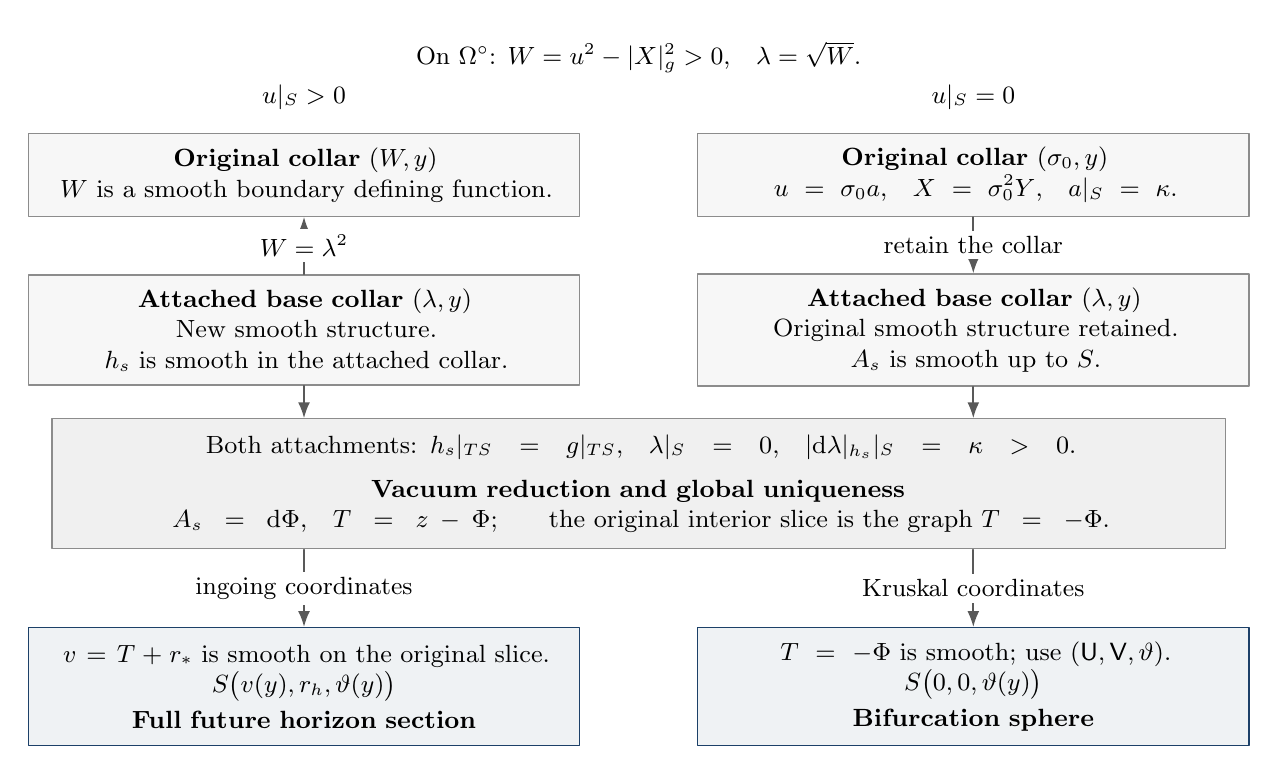
\begin{tikzpicture}[x=1cm,y=1cm,font=\small,
  line cap=round,line join=round,
  every node/.style={inner sep=5pt},
  box/.style={draw=black!45,fill=black!3,line width=.5pt,
    text width=6.65cm,align=center,minimum height=1.05cm},
  result/.style={box,draw=linkblue,fill=linkblue!7},
  flow/.style={-{Latex[length=2mm]},draw=black!65,line width=.6pt}]
  \node[anchor=south] at (7.9,8.0)
    {On $\Omega^\circ$: $W=u^2-|X|_g^2>0$,\quad $\lambda=\sqrt W$.};
  \node[anchor=south] at (3.65,7.53) {$u|_S>0$};
  \node[anchor=south] at (12.15,7.53) {$u|_S=0$};

  \node[box] (op) at (3.65,6.88)
    {\textbf{Original collar $(W,y)$}\\
     $W$ is a smooth boundary defining function.};
  \node[box] (oz) at (12.15,6.88)
    {\textbf{Original collar $(\sigma_0,y)$}\\
     $u=\sigma_0a$,\quad $X=\sigma_0^2Y$,\quad $a|_S=\kappa$.};

  \node[box,minimum height=1.3cm] (bp) at (3.65,4.91)
    {\textbf{Attached base collar $(\lambda,y)$}\\
     New smooth structure.\\
     $h_s$ is smooth in the attached collar.};
  \node[box,minimum height=1.3cm] (bz) at (12.15,4.91)
    {\textbf{Attached base collar $(\lambda,y)$}\\
     Original smooth structure retained.\\
     $A_s$ is smooth up to $S$.};
  \draw[flow] (bp.north)--(op.south)
    node[midway,fill=white,inner sep=2pt] {$W=\lambda^2$};
  \draw[flow] (oz.south)--(bz.north)
    node[midway,fill=white,inner sep=2pt] {retain the collar};

  \node[draw=black!45,fill=black!6,line width=.5pt,
    text width=14.55cm,align=center,minimum height=1.65cm]
    (global) at (7.9,2.96)
    {Both attachments: $h_s|_{TS}=g|_{TS}$,\quad $\lambda|_S=0$,\quad
      $|\dd\lambda|_{h_s}|_S=\kappa>0$.\\[5pt]
     \textbf{Vacuum reduction and global uniqueness}\\
     $A_s=\dd\Phi$,\quad $T=z-\Phi$;\qquad
     the original interior slice is the graph $T=-\Phi$.};
  \draw[flow] (bp.south)--(3.65,3.79);
  \draw[flow] (bz.south)--(12.15,3.79);

  \node[result,minimum height=1.5cm] (rp) at (3.65,.38)
    {$v=T+r_*$ is smooth on the original slice.\\
     $S\longmapsto\bigl(v(y),r_h,\vartheta(y)\bigr)$\\[2pt]
     \textbf{Full future horizon section}};
  \node[result,minimum height=1.5cm] (rz) at (12.15,.38)
    {$T=-\Phi$ is smooth; use $(\mathsf U,\mathsf V,\vartheta)$.\\
     $S\longmapsto\bigl(0,0,\vartheta(y)\bigr)$\\[2pt]
     \textbf{Bifurcation sphere}};
  \draw[flow] (3.65,2.12)--(rp.north)
    node[midway,fill=white,inner sep=2pt] {ingoing coordinates};
  \draw[flow] (12.15,2.12)--(rz.north)
    node[midway,fill=white,inner sep=2pt] {Kruskal coordinates};
\end{tikzpicture}
\caption{Boundary attachment and recovery of the original slice in the
connected nonextremal equality case. For positive boundary lapse, the upper
left arrow is the squaring correspondence from the attached collar to the
original collar; its inverse is not smooth at the boundary. For zero
boundary lapse, the original smooth structure is retained
(Lemma~\ref{stat:base-attachment}). The global primitive $\Phi$ enters only
after the uniqueness argument, as in \eqref{rec:global-time}. The two regular
spacetime extensions then recover the original $g,K,E$, by
\eqref{rec:ingoing}, \eqref{rec:kruskal}, and
Proposition~\ref{rec:original-embedding}.}
\label{rec:fig-boundary-recovery}
\end{figure}


\begin{proposition}[Converse and sharpness]\label{rec:sharpness}
Every model slice in the stated converse class, with parameters
$M>|q_0|$ and actual invariant ADM mass and signed flux equal to
$M,q_0$, attains equality. For every such parameter pair and every
$n\geq4$, this class contains the static exterior slice and smooth
compact radial time perturbations of it with $K\not\equiv0$.
\end{proposition}

\begin{proof}
Let
\[
 r_+^{k-1}=M+\sqrt{M^2-q_0^2}.
\]
The degenerate metric on the future horizon is $r_+^2\sigma_k$
on its generator labels, independently of the position along a
generator. Thus a full section, including the bifurcation sphere,
has area $\omega r_+^k$. The assumed lower bound for all full
cuts, and the fact that the boundary is itself a full cut, give
\[
 A_{\min}=\Area_g(S)=\omega r_+^k.
\]
Using the actual mass and signed charge specified in the converse
now gives the equality formula. This argument does not identify
the ADM parameters of arbitrary unqualified model slices.

We verify the advertised examples, including their geometric
hypotheses. Put
\[
 f=1-2Mr^{-(k-1)}+q_0^2r^{-2k+2}.
\]
The static $T=0$ slice has
\begin{equation}\label{rec:static-example}
 g=f^{-1}\dd r^2+r^2\sigma_k,\quad K=0,\quad
 E=q_0r^{-k}\sqrt f\,\partial_r,
 \qquad r\geq r_+.
\end{equation}
The simple root makes the boundary a regular bifurcation sphere:
in proper distance $s\geq0$,
$r-r_+=f'(r_+)s^2/4+O(s^4)$. Thus $g$ and $E$ are smooth
to the boundary and complete with it included. The boundary is
totally geodesic and future marginal.

The ambient metric and field obey the stated Einstein--Maxwell
normalization in every dimension. For an explicit check, their
time and radial mixed Ricci eigenvalues are
\[
 -\tfrac12f''-\frac{k}{2r}f'
        =-(k-1)^2q_0^2r^{-2k},
\]
and their angular mixed eigenvalue is
\[
 \frac{(k-1)(1-f)-rf'}{r^2}
        =(k-1)q_0^2r^{-2k}.
\]
With $c_n^2=k(k-1)/2$, these are exactly
$\Ric_{ab}=2F_{ac}F_b{}^c-(F_{cd}F^{cd}/k)G_{ab}$.
The Faraday form is closed, and its spacetime dual has constant
sphere flux, hence is closed as well. Gauss--Codazzi and these
Maxwell equations give $\mu_m=J_m=0$ and $\Div E=0$ on every
spacelike slice with the prescribed induced fields and vanishing
induced magnetic two-form.

For a nonstatic example choose a smooth nonconstant
$\tau(r)$ compactly supported in an interval
$r_++\delta<r<R$, and use the graph $T=\tau(r)$. After multiplying
$\tau$ by a sufficiently small constant it is spacelike, since
\begin{equation}\label{rec:radial-graph}
 g_\tau=a(r)\,\dd r^2+r^2\sigma_k,
 \qquad a=f^{-1}-f(\tau')^2>0.
\end{equation}
Near the boundary and infinity this is exactly the static slice.
Its magnetic two-form vanishes identically, because
\[
 \iota^*(\dd T\wedge\dd r)
      =\tau'(r)\,\dd r\wedge\dd r=0.
\]
Its normalized electric flux is $q_0$ by Maxwell closure. For
example its electric field is
$q_0r^{-k}a^{-1/2}\partial_r$, as follows by contracting the
Faraday form with its future unit normal.

The end is unchanged. Its momentum is zero, and its energy is
$M$: in asymptotic Cartesian coordinates the metric perturbation
is $(f^{-1}-1)n_i n_j$, with
$f^{-1}-1=2Mr^{-(n-2)}+O(r^{-2(n-2)})$. The ADM integrand has
radial component $(n-1)(f^{-1}-1)/r$, giving precisely $M$
with the normalization $[2(n-1)\omega]^{-1}$. All required
asymptotic derivative bounds and integrability statements follow.

Every full cut has area at least $\omega r_+^k$. Indeed angular
projection onto the boundary sphere has differential whose
$k$-dimensional Jacobian is at most $(r_+/r)^k\leq1$ for the
metric \eqref{rec:radial-graph}, regardless of its positive radial
coefficient. The integral of the pullback boundary volume form
over an end-oriented full cut is $\omega r_+^k$, by Stokes on
the compact region between the cut and a large round sphere.
This remains valid for disconnected cuts and portions on the
original boundary, with their full intrinsic boundary counted.
The comass bound for that pullback form proves the area lower
bound. The boundary attains it.

There is also no smooth interior full weakly future trapped cut.
For clarity its exclusion can be checked directly for every
spacelike radial graph above. Its outward unit normal within the
slice is $a^{-1/2}(\partial_r+\tau'\partial_T)$, while its future
unit spacetime normal is
\[
 N=\frac{f^{-1}}{\sqrt a}\,\partial_T
       +\frac{f\tau'}{\sqrt a}\,\partial_r.
\]
The round sphere expansion is consequently
\begin{equation}\label{rec:round-expansion}
 \theta_+(r)=\frac{k}{r\sqrt a}(1+f\tau')>0
 \qquad(r>r_+),
\end{equation}
because spacelikeness gives $|f\tau'|<1$. If an interior compact
full cut were weakly future trapped, take a point where its radial
coordinate is maximal. The full exterior it bounds contains every
point with larger radius, so its end-oriented normal at that point
is the outward radial normal. It is tangent there to its enclosing
round sphere from the inside. The graph mean-curvature comparison
gives $H_{\mathrm{cut}}\geq H_{\mathrm{sphere}}$ at contact,
and their tangential traces of $K$ agree because the tangent
planes agree. Equation~\eqref{rec:round-expansion} contradicts
weak future trapping. This uses the full-cut condition to fix the
normal also when the cut is disconnected.

Finally choose $\tau$ with $\tau'(r_0)=0$ and
$\tau''(r_0)\ne0$ at some interior point. At that point the
radial second fundamental form component of the graph is
$K_{rr}=\sqrt{f(r_0)}\,\tau''(r_0)$ with the stipulated future
normal convention. Thus $K$ is nonzero. These examples satisfy
all the connected-horizon hypotheses, have the same area, energy,
momentum and signed charge as the static examples, and attain
equality.
\end{proof}


\begin{proof}[Completion of Theorems~\ref{thm:rigidity} and~\ref{thm:converse}]
Proposition~\ref{rec:original-embedding} proves the Original-Data
Rigidity Theorem~\ref{thm:rigidity}. Proposition~\ref{rec:sharpness}
proves the Converse and Sharp Examples Theorem~\ref{thm:converse},
including the nonstatic purely electric examples.
\end{proof}

\bibliographystyle{plainnat}
\bibliography{references}
\end{document}
